%%%%%%%%%%%%%%%%%%%%%%%%%%%%%%%%%%%%%%%%%%%%%%%%%%%%%%%%%%%%%%%%%%%%%%%%%%%%
%                                                                          %
%              (C) Copyright 1995 The Board of Trustees of the             %
%                          University of Illinois                          %
%                           All Rights Reserved                            %
%								  	   %
%%%%%%%%%%%%%%%%%%%%%%%%%%%%%%%%%%%%%%%%%%%%%%%%%%%%%%%%%%%%%%%%%%%%%%%%%%%%

\documentclass[11pt]{article}
\usepackage{graphicx}
\usepackage{makeidx}
\usepackage{amssymb}
\usepackage{amsmath}
\usepackage{verbatim}
\usepackage{comment}
\usepackage[stable]{footmisc}
%\usepackage{hyperref}  % links in table of contents
%\usepackage{tocloft}
\makeindex

% define margins, etc
\topmargin	0.1in
\oddsidemargin	0in
\evensidemargin	0in
\textheight	8.80in
\textwidth	6.50in
\marginparsep	0.25cm
\headheight	0in
\headsep	0in
%\footskip	0.5in
%\footheight	0in%

% define macros
%%%%%%%%%%%%%%%%%%%%%%%%%%%%%%%%%%%%%%%%%%%%%%%%%%%%%%%%%%%%%%%%%%%%%%%%%%%%
%                                                                          %
%              (C) Copyright 1995 The Board of Trustees of the             %
%                          University of Illinois                          %
%                           All Rights Reserved                            %
%								  	   %
%%%%%%%%%%%%%%%%%%%%%%%%%%%%%%%%%%%%%%%%%%%%%%%%%%%%%%%%%%%%%%%%%%%%%%%%%%%%

%
% generally useful macros
%
\newcommand{\REFAND} {\&}
\newcommand{\ETALNP}{\mbox{\it et al}}
\newcommand{\ETAL}{\mbox{\ETALNP{\it.}}}
\newcommand{\eqnref}[1] {\mbox{eq (\ref{#1})}}
\newcommand{\mycite}[2] {\cite{#2}}
%\newcommand{\mycite}[2] {}

\newcommand{\NAMD} {NAMD}
\newcommand{\NAMDDATE} {\today}
\newcommand{\NAMDAUTHORS} {M.~Bhandarkar, A.~Bhatele, E.~Bohm, R.~Brunner, F.~Buelens, C.~Chipot, A.~Dalke, S.~Dixit, G.~Fiorin, P.~Freddolino, P.~Grayson, J.~Gullingsrud, A.~Gursoy, D.~Hardy, C.~Harrison, J.~H\'enin, W.~Humphrey, D.~Hurwitz, N.~Krawetz, S.~Kumar, D.~Kunzman, J.~Lai, C.~Lee, R.~McGreevy, C.~Mei, M.~Nelson, J.~Phillips, O.~Sarood, A.~Shinozaki, D.~Tanner, D.~Wells, G.~Zheng, F.~Zhu}

% The file namd_version.tex is automatically generated by the Makefile.
\input{namd_version}

%
% macros for style conventions when describing the program.
%

% name of class or object in program
\newcommand{\OBJ}[1] {{\bf\tt#1}}

% function arguments
\newcommand{\FA}[2] {{\rm{\bf#1}\ {\it#2}}}

% global function name
\newcommand{\FN}[3] {{\rm\bf#1}\ {\tt #2(}#3{\tt)}}

% class member function name
\newcommand{\FNO}[4] {{\rm\bf#2}\ \OBJ{#1::}{\tt#3(}#4{\tt)}}

% list item, for optional components, parameters, etc.
\newcommand{\TTLISTITEM}[1] {\item {\tt #1} \\}
\newcommand{\RMLISTITEM}[1] {\item {\rm #1} \\}
\newcommand{\BOLDLISTITEM}[1] {\item {\bf #1} \\}
\newcommand{\EMLISTITEM}[1] {\item {\em #1} \\}
\newcommand{\LISTITEM}[1] {\RMLISTITEM{#1}}

%
% other generally useful macros
%

% Other program names, formatted nicely
\newcommand{\FEP} {FEP}
\newcommand{\VMD} {VMD}
\newcommand{\MDCOMM} {MDComm}
\newcommand{\MDSCOPE} {MDScope}
\newcommand{\CESB} {MDScope}
\newcommand{\ALLNAMES} {MDScope}
\newcommand{\SMALLMDSCOPE} {mdscope}
\newcommand{\SMALLCESB} {mdscope}
\newcommand{\SMALLALLNAMES} {mdscope}

% full name for MDScope, i.e., what it stands for
\newcommand{\MDSCOPENAME} {Molecular Dynamics computational environment}

% title of MDScope paper
\newcommand{\MDSCOPEPAPER} {MDScope: A Visual Computing Environment for
Structural Biology}

% default definitions for title and description
% \newcommand{\DOCTITLE} {Documentation Guides}
% \newcommand{\DOCDESC} {
%   This document includes the \NAMD\ Installation, Users, and
% Programmers Guides, which document how to obtain, install, use, and
% modify the molecular graphics program \NAMD.}


\newcommand{\VMD} {VMD}
\newcommand{\NAMD} {NAMD}
\newcommand{\PSFGEN} {{\tt psfgen}}
\newcommand{\PSFGENVER} {1.6}
\newcommand{\PSFGENAUTHORS} {\tt Justin Gullingsrud, Jan Saam, and Jim Phillips}

%
% generally useful macros
%
\newcommand{\REFAND} {\&}
\newcommand{\ETALNP}{\mbox{\it et al}}
\newcommand{\ETAL}{\mbox{\ETALNP{\it.}}}
\newcommand{\eqnref}[1] {\mbox{eq (\ref{#1})}}
\newcommand{\mycite}[2] {\cite{#2}}

%
% macros for style conventions when describing the program.
%

% name of class or object in program
\newcommand{\OBJ}[1] {{\bf\tt#1}}

% function arguments
\newcommand{\FA}[2] {{\rm{\bf#1}\ {\it#2}}}

% global function name
\newcommand{\FN}[3] {{\rm\bf#1}\ {\tt #2(}#3{\tt)}}

% class member function name
\newcommand{\FNO}[4] {{\rm\bf#2}\ \OBJ{#1::}{\tt#3(}#4{\tt)}}

% list item, for optional components, parameters, etc.
\newcommand{\TTLISTITEM}[1] {\item {\tt #1} \\}
\newcommand{\RMLISTITEM}[1] {\item {\rm #1} \\}
\newcommand{\BOLDLISTITEM}[1] {\item {\bf #1} \\}
\newcommand{\EMLISTITEM}[1] {\item {\em #1} \\}
\newcommand{\LISTITEM}[1] {\RMLISTITEM{#1}}


\newcommand{\eg}{{\it e.g.\/}}
\newcommand{\ie}{{\it i.e.\/}}

\newcommand{\KEY}[1]{{\tt #1}}
\newcommand{\IKEY}[1]{{\tt #1\index{#1 psfgen command}}}
\newcommand{\OKEY}[1]{$[${\tt #1}$]$}
\newcommand{\ARG}[1]{$<${\em #1}$>$}
\newcommand{\OARG}[1]{$[${\em #1}$]$}
\newcommand{\ARGDEF}[2]{$<${\em #1}$>$: #2}
\newcommand{\KEYDEF}[2]{{\tt #1}: #2}
\newcommand{\COMMAND}[4]{%
  #1 \\ {\bf Purpose:} #2 \\ {\bf Arguments:} #3 \\ {\bf Context:} #4 }


\input{psfgen_macros}

\includecomment{cvnamd}
\excludecomment{cvlammps}
\excludecomment{cvrefman}

\begin{cvnamd}

% compiling the NAMD User's Guide

% define missing macros
\newcommand{\MDENGINE}{NAMD}
\newcommand{\cvrefmanonly}[1]{}
\newcommand{\cvnamdonly}[1]{#1}
\newcommand{\cvnamebasedonly}[1]{#1}
\newcommand{\cvlammpsonly}[1]{}
\newcommand{\cvnamdugonly}[1]{#1}

% use the NAMD UG macros to document keywords
\newcommand{\key}[5]{\NAMDCONF{#1}{(#2 context) #3}{#4}{#5}}
\newcommand{\keydef}[6]{\NAMDCONFWDEF{#1}{(#2 context) #3}{#4}{#5}{#6}}

\newcommand{\cvsec}[1]{\subsection{#1}}
\newcommand{\cvsubsec}[1]{\subsubsection{#1}}
\newcommand{\cvsubsubsec}[1]{\paragraph*{#1}}

\end{cvnamd}

\begin{cvrefman}

% compiling the standalone reference manual

% use macros with context field to document keywords
\newcommand{\key}[5]{%
  \index{\texttt{#1}}
  {\bf \large \tt #1 } $\langle\,$#3$\,\rangle$ \\%
  {\bf Context: } #2 \\%
  {\bf Acceptable values: } #4 \\%
  {\bf Description: } #5%
}
\newcommand{\keydef}[6]{%
  \index{\texttt{#1}}
  {\bf \large \tt #1 } $\langle\,$#3$\,\rangle$ \\%
  {\bf Context: } #2 \\%
  {\bf Acceptable values: } #4 \\%
  {\bf Default value: } #5 \\%
  {\bf Description: } #6%
}
\newcommand{\gradx}{\mbox{\boldmath$\nabla_{\!\!x}\,$}}
\newcommand{\vx}{{\mbox{\boldmath{$x$}}}}
\newcommand{\bm}[1]{{\mbox{\boldmath{$#1$}}}}

\newcommand{\cvsec}[1]{\section{#1}}
\newcommand{\cvsubsec}[1]{\subsection{#1}}
\newcommand{\cvsubsubsec}[1]{\subsubsection{#1}}

\end{cvrefman}

\begin{cvnamd}
\newcommand{\outputName}{\emph{outputName}}
\newcommand{\restartName}{\emph{restartName}}
\newcommand{\inputName}{\emph{inputName}}
\end{cvnamd}

\begin{cvlammps}
\newcommand{\outputName}{\emph{output}}
\newcommand{\restartName}{\emph{restart}}
\newcommand{\inputName}{\emph{input}}
\end{cvlammps}



\setcounter{secnumdepth}{3}
%% \setcounter{tocdepth}{5} %% very detailed table of contents
\setcounter{tocdepth}{4}

%
% the document itself
%


\begin{document}

% strictly enforce margins rather than complaining
\sloppy

% initial pages for the guide - title, TOC, etc.
%%%%%%%%%%%%%%%%%%%%%%%%%%%%%%%%%%%%%%%%%%%%%%%%%%%%%%%%%%%%%%%%%%%%%%%%%%%%
%                                                                          %
%              (C) Copyright 1995 The Board of Trustees of the             %
%                          University of Illinois                          %
%                           All Rights Reserved                            %
%								  	   %
%%%%%%%%%%%%%%%%%%%%%%%%%%%%%%%%%%%%%%%%%%%%%%%%%%%%%%%%%%%%%%%%%%%%%%%%%%%%

% title page

\thispagestyle{empty}

\vspace*{0.3in}

\begin{centering}
  \rule{6in}{0.04in}				\\	\vspace{0.25in}
  {\Huge \NAMD\ \DOCTITLE}			\\	\vspace{0.25in}
  {\Large Version \NAMDVER}			\\	\vspace{0.20in}
  \rule{6in}{0.04in}				\\	\vspace{0.25in}
  {\Large \NAMDAUTHORS}				\\	\vspace{0.20in}
  \NAMDDATE					\\	\vspace{0.20in}
  \rule{6in}{0.04in}				\\	\vspace{0.25in}
  {\large       Theoretical Biophysics Group}                  \\ 
  {\large       University of Illinois and Beckman Institute}  \\ 
  {\large       405 N. Mathews}                                \\ 
  {\large       Urbana, IL  61801}                             \\
\end{centering}
\vspace{0.2in}

\begin{center}
  {\Large \bf Description}
\end{center}

\noindent \DOCDESC



% copyright and permissions notices
\newpage

\thispagestyle{empty}

\vspace*{0.1in}

\begin{centering}
{\LARGE \NAMD\ Version \NAMDVER}\\
\bigskip
{\large Authors: \NAMDAUTHORS} \\
\medskip
{\large Theoretical Biophysics Group, Beckman Institute, University of Illinois.} \\
\bigskip
{\large \copyright 1995-2011 The Board of Trustees of the University of Illinois.
All Rights Reserved} \\
\bigskip
\end{centering}

  \rule{6in}{0.04in}				\\	\vspace{0.25in}

\section*{NAMD Molecular Dynamics Software \\
Non-Exclusive, Non-Commercial Use License}

\subsubsection*{Introduction}

The University of Illinois at Urbana-Champaign has created its molecular
dynamics software, NAMD, developed by the Theoretical Biophysics 
Group (``TBG'') at Illinois' Beckman Institute available free of charge for
non-commercial use by individuals, academic or research institutions and
corporations for in-house business purposes only, upon completion and
submission of the online registration form presented when attempting to
download NAMD at the web site {\tt http://www.ks.uiuc.edu/Research/namd/}.

Commercial use of the NAMD software, or derivative works based thereon,
REQUIRES A COMMERCIAL LICENSE. Commercial use includes: 
(1) integration of all or part of the Software into a product for sale, 
lease or license by or on behalf of Licensee to third parties, or 
(2) distribution of the Software to third parties that need it to 
commercialize product sold or licensed by or on behalf of Licensee.  
The University of Illinois will negotiate commercial-use licenses for 
NAMD upon request. These requests can be directed to namd@ks.uiuc.edu

\subsubsection*{Online Download Registration Requirements}

In completing the online registration form presented before downloading
individuals may register in their own name or with their institutional or
corporate affiliations. Registration information must include name, title, 
and e-mail of a person with signature authority to authorize and commit the
individuals, academic or research institution, or corporation as necessary 
to the terms and conditions of the license agreement.

All parts of the information must be understood and agreed to as part of
completing the form. Completion of the form is required before software 
access is granted. Pay particular attention to the authorized requester 
requirements above, and be sure that the form submission is authorized 
by the duly responsible person.

\newpage
\subsubsection*{UNIVERSITY OF ILLINOIS \\
NAMD MOLECULAR DYNAMICS SOFTWARE LICENSE AGREEMENT}

Upon execution of this Agreement by the party identified below (``Licensee''),
The Board of Trustees of the University of Illinois (``Illinois''), on 
behalf of The Theoretical Biophysics Group (``TBG'') in the Beckman Institute,
will provide the molecular dynamics software NAMD in Executable 
Code and/or Source Code form (``Software'') to Licensee, subject to 
the following terms and conditions. For purposes of this Agreement, 
Executable Code is the compiled code, which is ready to run on Licensee's 
computer. Source code consists of a set of files which contain the 
actual program commands that are compiled to form the Executable Code.

1. The Software is intellectual property owned by Illinois, and all 
right, title and interest, including copyright, remain with Illinois. 
Illinois grants, and Licensee hereby accepts, a restricted, non-exclusive, 
non-transferable license to use the Software for academic, research 
and internal business purposes only e.g. not for commercial use 
(see Paragraph 7 below), without a fee. Licensee agrees to reproduce 
the copyright notice and other proprietary markings on all copies of 
the Software. Licensee has no right to transfer or sublicense the 
Software to any unauthorized person or entity. However, Licensee does 
have the right to make complimentary works that interoperate with NAMD, 
to freely distribute such complimentary works, and to direct others 
to the TBG server to obtain copies of NAMD itself.

2. Licensee may, at its own expense, modify the Software to make derivative
works, for its own academic, research, and internal business purposes.
Licensee's distribution of any derivative work is also subject to the same
restrictions on distribution and use limitations that are specified herein
for Illinois' Software. Prior to any such distribution the Licensee shall 
require the recipient of the Licensee's derivative work to first execute a 
license for NAMD with Illinois in accordance with the terms and conditions 
of this Agreement. Any derivative work should be clearly marked and 
renamed to notify users that it is a modified version and not the original 
NAMD code distributed by Illinois.

3. Except as expressly set forth in this Agreement, THIS SOFTWARE IS 
PROVIDED ``AS IS'' AND ILLINOIS MAKES NO REPRESENTATIONS AND EXTENDS NO 
WARRANTIES OF ANY KIND, EITHER EXPRESS OR IMPLIED, INCLUDING BUT NOT 
LIMITED TO WARRANTIES OR MERCHANTABILITY OR FITNESS FOR A PARTICULAR 
PURPOSE, OR THAT THE USE OF THE SOFTWARE WILL NOT INFRINGE ANY PATENT, 
TRADEMARK, OR OTHER RIGHTS. LICENSEE ASSUMES THE ENTIRE RISK AS TO 
THE RESULTS AND PERFORMANCE OF THE SOFTWARE AND/OR ASSOCIATED MATERIALS. 
LICENSEE AGREES THAT UNIVERSITY SHALL NOT BE HELD LIABLE FOR ANY DIRECT, 
INDIRECT, CONSEQUENTIAL, OR INCIDENTAL DAMAGES WITH RESPECT TO ANY 
CLAIM BY LICENSEE OR ANY THIRD PARTY ON ACCOUNT OF OR ARISING FROM 
THIS AGREEMENT OR USE OF THE SOFTWARE AND/OR ASSOCIATED MATERIALS.

4. Licensee understands the Software is proprietary to Illinois. 
Licensee agrees to take all reasonable steps to insure that the Software 
is protected and secured from unauthorized disclosure, use, or release 
and will treat it with at least the same level of care as Licensee would 
use to protect and secure its own proprietary computer programs and/or 
information, but using no less than a reasonable standard of care. 
Licensee agrees to provide the Software only to any other person or 
entity who has registered with Illinois. If licensee is not registering 
as an individual but as an institution or corporation each member of 
the institution or corporation who has access to or uses Software must 
understand and agree to the terms of this license. If Licensee becomes 
aware of any unauthorized licensing, copying or use of the Software, 
Licensee shall promptly notify Illinois in writing. Licensee expressly 
agrees to use the Software only in the manner and for the specific uses 
authorized in this Agreement.

5. By using or copying this Software, Licensee agrees to abide by the
copyright law and all other applicable laws of the U.S. including, but 
not limited to, export control laws and the terms of this license. 
Illinois shall have the right to terminate this license immediately by 
written notice upon Licensee's breach of, or non-compliance with, any 
of its terms. Licensee may be held legally responsible for any copyright 
infringement that is caused or encouraged by its failure to abide by 
the terms of this license. Upon termination, Licensee agrees to destroy 
all copies of the Software in its possession and to verify such 
destruction in writing.

6. The user agrees that any reports or published results obtained 
with the Software will acknowledge its use by the appropriate citation 
as follows: 

\begin{quote}
 NAMD was developed by the Theoretical Biophysics Group in the 
 Beckman Institute for Advanced Science and Technology at the 
 University of Illinois at Urbana-Champaign.
\end{quote}

Any published work which utilizes NAMD shall include the following reference: 

\begin{quote}
 James C. Phillips, Rosemary Braun, Wei Wang, James Gumbart,
 Emad Tajkhorshid, Elizabeth Villa, Christophe Chipot, Robert D. Skeel,
 Laxmikant Kale, and Klaus Schulten. Scalable molecular dynamics with NAMD.
 {\it Journal of Computational Chemistry}, 26:1781-1802, 2005.
\end{quote}

Electronic documents will include a direct link to the official NAMD page:

\begin{quote}
{\tt http://www.ks.uiuc.edu/Research/namd/}
\end{quote}

One copy of each publication or report will be supplied to Illinois 
at the addresses listed below in Contact Information.

7. Should Licensee wish to make commercial use of the Software, Licensee 
will contact Illinois (namd@ks.uiuc.edu) to negotiate an appropriate 
license for such use. Commercial use includes: (1) integration of all 
or part of the Software into a product for sale, lease or license by or 
on behalf of Licensee to third parties, or (2) distribution of the 
Software to third parties that need it to commercialize product sold or 
licensed by or on behalf of Licensee.

8. Government Rights. Because substantial governmental funds have been 
used in the development of NAMD, any possession, use or sublicense of 
the Software by or to the United States government shall be subject 
to such required restrictions.

9. NAMD is being distributed as a research and teaching tool and as such, 
TBG encourages contributions from users of the code that might, at 
Illinois' sole discretion, be used or incorporated to make the basic 
operating framework of the Software a more stable, flexible, and/or 
useful product. Licensees that wish to contribute their code to become 
an internal portion of the Software may be required to sign an 
``Agreement Regarding Contributory Code for NAMD Software''
before Illinois can accept it (contact namd@ks.uiuc.edu for a copy).

\newpage
\subsubsection*{Contact Information}

The best contact path for licensing issues is by e-mail to namd@ks.uiuc.edu
or send correspondence to:
\begin{verse}
                             NAMD Team\\
                             Theoretical Biophysics Group\\
                             Beckman Institute\\
                             University of Illinois\\
                             405 North Mathews MC-251\\
                             Urbana, Illinois 61801 USA\\
                             FAX: (217) 244-6078
\end{verse}




% table of contents
\newpage
\tableofcontents

% list of figures
\newpage
\listoffigures

% list of tables
% \listoftables
%
% There are currently NO tables in either the User Guide or 
% the Programmer's Guide.  
%

\newpage


% Introduction
%%%%%%%%%%%%%%%%%%%%%%%%%%%%%%%%%%%%%%%%%%%%%%%%%%%%%%%%%%%%%%%%%%%%%%%%%%%%
%                                                                          %
%              (C) Copyright 1995 The Board of Trustees of the             %
%                          University of Illinois                          %
%                           All Rights Reserved                            %
%								  	   %
%%%%%%%%%%%%%%%%%%%%%%%%%%%%%%%%%%%%%%%%%%%%%%%%%%%%%%%%%%%%%%%%%%%%%%%%%%%%


\section{Introduction}
\label{section:intro}

\NAMD\ is a parallel molecular dynamics program for UNIX 
platforms designed for high-performance 
simulations in structural biology.  This document describes how to use 
\NAMD, its features, and the platforms on which it runs.
The document is divided into several sections:
\begin{description}
\item[Section \ref{section:intro}] gives an overview of \NAMD.
\item[Section \ref{section:start}] lists the basics for getting started.
\item[Section \ref{section:files}] describes \NAMD\ file formats.
\item[Section \ref{section:psfgen}] explains PSF file generation with psfgen.
\item[Section \ref{section:forcefield}] presents the potential functions,
non-bonded interactions, and full electrostatics.
\item[Section \ref{section:gbis}] explains Generalized Born implicit solvent simulations. 
\item[Section \ref{section:dynamics}] lists standard minimization
and dynamics parameters.
\item[Section \ref{section:performance}] lists performance tuning parameters.
\item[Section \ref{section:userdef}] explains user defined forces.
% \item[Section \ref{section:fenergy}] discusses free energy of
conformation change calculations.
\item[Section \ref{section:colvars}] describes collective
variable-based calculations.
\item[Section \ref{section:alchemy}] explains alchemical free energy calculations.
\item[Section \ref{section:accel}] presents accelerated sampling methods.
\item[Section \ref{section:analysis}] lists runtime analysis options.
\item[Section \ref{section:xplorequiv}] provides hints for X-PLOR users.
\item[Section \ref{section:sample}] provides sample configuration files.
\item[Section \ref{section:run}] gives details on running \NAMD.
\item[Section \ref{section:avail}] gives details on installing \NAMD.
\end{description}


\subsection{\NAMD\ and molecular dynamics simulations}

Molecular dynamics (MD) simulations compute atomic trajectories by solving
equations of motion numerically using empirical force fields, such as the 
CHARMM force field, that approximate the actual atomic force in 
biopolymer systems. Detailed information about MD simulations can be found in
several books such as 
\mycite{(Allen and Tildesley),(McCammon and Harvey)}{ALLE87,MCCA87}. 
In order to conduct MD simulations, various computer programs have been 
developed including
X-PLOR \mycite{(Br\"unger, 1992)}{BRUN92b} and 
CHARMM \mycite{(Brooks \ETAL, 1983)}{BROO83}.
These programs were originally developed for serial machines. 
Simulation of large molecules, however, require enormous computing power. 
One way to achieve such simulations is to utilize parallel computers. In recent 
years, distributed memory parallel computers have been offering
cost-effective computational power.  \NAMD\ was designed to run efficiently
on such parallel 
machines for simulating large molecules. 
\NAMD\ is particularly well suited to the increasingly popular Beowulf-class PC clusters, which are quite similar to the workstation clusters for which is was originally designed.
Future versions of \NAMD\ will also make efficient use of clusters of multi-processor workstations or PCs.
\prettypar
\NAMD\ has several important features: 

\begin{itemize}

\item{\bf Force Field Compatibility}\\
The force field used by \NAMD\ is the same as that used by the programs 
CHARMM \mycite{(Brooks \ETAL, 1983)}{BROO83} and X-PLOR 
\mycite{(Br\"unger, 1992)}{BRUN92b}.  This force field includes local 
interaction terms consisting of bonded interactions between 2, 3, and 4 atoms 
and pairwise interactions including electrostatic and van der Waals forces.
This commonality allows simulations to migrate between these three programs.

\item{\bf Efficient Full Electrostatics Algorithms}\\
\NAMD\ incorporates the Particle Mesh Ewald (PME) algorithm,
which takes the full electrostatic interactions into account.
This algorithm reduces the computational complexity of electrostatic
force evaluation from $O(N^2)$ to $O(N \log N)$.

\item{\bf Multiple Time Stepping}\\
The velocity Verlet integration method
\mycite{M. P. Allen and D. J. Tildesley, 1987}{ALLE87}
is used to advance the positions and velocities of the atoms in time.
To further reduce the cost of the evaluation of 
long-range electrostatic forces, 
a multiple time step scheme is employed.  The local
interactions (bonded, van der Waals and electrostatic interactions within a
specified distance) are calculated at each time step.  The longer range
interactions (electrostatic interactions beyond the specified distance) are
only computed less often.
This amortizes the cost of computing the electrostatic forces over several timesteps.
A smooth splitting function is used to separate a quickly varying short-range portion of the electrostatic interaction from a more slowly varying long-range component.
It is also possible to employ an intermediate timestep for the short-range non-bonded interactions, performing only bonded interactions every timestep.


\item{\bf Input and Output Compatibility}\\
The input and output file formats used by \NAMD\ are identical to those
used by CHARMM and X-PLOR.  Input formats include coordinate files in PDB format
\mycite{(Bernstein \ETAL, 1977)}{BERN77}, structure files in X-PLOR PSF format, 
and energy parameter files in either ~CHARMM or X-PLOR formats.
Output formats include PDB coordinate files and binary DCD trajectory files.
These similarities assure that the molecular dynamics trajectories from \NAMD\ 
can be read by CHARMM or X-PLOR and that the user can exploit the many 
analysis algorithms of the latter packages.

\item{\bf Dynamics Simulation Options}\\
MD simulations may be carried out using several options, including
\begin{itemize}
  \item Constant energy dynamics,
  \item Constant temperature dynamics via
  \begin{itemize}
    \item Velocity rescaling,
    \item Velocity reassignment,
    \item Langevin dynamics,
  \end{itemize}
  \item Periodic boundary conditions,
  \item Constant pressure dynamics via
  \begin{itemize}
    \item Berendsen pressure coupling,
    \item Nos\'{e}-Hoover Langevin piston,
  \end{itemize}
  \item Energy minimization,
  \item Fixed atoms,
  \item Rigid waters,
  \item Rigid bonds to hydrogen,
  \item Harmonic restraints,
  \item Spherical or cylindrical boundary restraints.
\end{itemize}

\item{\bf Easy to Modify and Extend}\\
Another primary design objective for \NAMD\ is extensibility and 
maintainability. In order to achieve this, it is designed in an 
object-oriented style with C++. Since molecular dynamics is a new field,
new algorithms and techniques are continually being developed.
\NAMD's modular design allows one to integrate and test new algorithms 
easily.  If you are contemplating a particular modification to \NAMD\
you are encouraged to contact the developers for guidance.

\item{\bf Interactive MD simulations}\\
A system undergoing simulation in \NAMD\ may be viewed and
altered with \VMD; for instance, forces can be applied to a set of atoms
to alter or rearrange part of the molecular structure.  For more information
on \VMD, see {\tt http://www.ks.uiuc.edu/Research/vmd/}.  

\item{\bf Load Balancing}\\
An important factor in parallel applications is the equal distribution
of computational load among the processors. In parallel molecular simulation,
a spatial decomposition that evenly distributes the computational load
causes the region of space mapped to each processor to become very irregular, 
hard to compute and difficult to generalize to the evaluation of many different
types of forces.  \NAMD\ addresses this problem by using a simple uniform 
spatial decomposition where the entire model is split into uniform cubes of 
space called {\em patches}. An initial load balancer assigns patches
and the calculation of interactions among the atoms within them
to processors such that the computational load is balanced as much as possible.
During the simulation, an incremental load balancer monitors the load
and performs necessary adjustments.

\end{itemize}

\subsection{Acknowledgments}

This work is supported by grants from the National Science
Foundation (BIR-9318159) and the National Institute of Health 
(PHS 5 P41 RR05969-04).
\prettypar
The authors would particularly like to thank the members of the
Theoretical Biophysics Group, past and present, who have helped
tremendously in making suggestions, pushing for new features, and
testing bug-ridden code.



% Getting started
\newpage

\section{Getting Started}
\label{section:start}

\subsection{What is needed}

Before running \NAMD, explained in section \ref{section:run}, 
the following are be needed:
\begin{itemize}
\item A CHARMM force field in either CHARMM or X-PLOR format.
\item
An X-PLOR format PSF file describing the molecular structure.
\item
The initial coordinates of the molecular system in the form of a PDB file.  
\item
A \NAMD\ configuration file.
\end{itemize}

\NAMD\ provides the \verb#psfgen# utility,
documented in Section~\ref{section:psfgen},
which is capable of generating the required PSF and PDB files by
merging PDB files and guessing coordinates for missing atoms.
If \verb#psfgen# is insufficient for your system,
we recommend that you obtain access to either CHARMM or X-PLOR,
both of which are capable of generating the required files.

\subsection{\NAMD\ configuration file}
\label{section:config}

Besides these input and output files, \NAMD\ also uses 
a file referred to as the {\it configuration file\/}.  
This file specifies what dynamics options and values that 
\NAMD\ should use, such as the number of timesteps to perform, 
initial temperature, etc.  
The options and values in this file control how 
the system will be simulated.  

A \NAMD\ configuration file contains a set of options and values.  
The options and values specified determine the exact behavior of
\NAMD, what features are active or inactive, how long the simulation
should continue, etc.  Section \ref{section:configsyntax} describes how
options are specified within a \NAMD\ configuration file.  Section
\ref{section:requiredparams} lists the parameters which are required
to run a basic simulation.  Section \ref{section:xplorequiv}
describes the relation between specific \NAMD\ and X-PLOR dynamics
options.  Several sample \NAMD\ configuration files are shown
in section \ref{section:sample}.


\subsubsection{Configuration parameter syntax}
\label{section:configsyntax}
Each line
in the configuration files consists of a $keyword$ identifying the option
being specified, and a $value$ which is a parameter to be used for this
option.  The keyword and value can be separated by only white space:
\begin{verbatim}
keyword            value
\end{verbatim}
or the keyword and value can be separated by an equal sign and white space:
\begin{verbatim}
keyword      =     value
\end{verbatim}
Blank lines in the configuration file are ignored.  Comments are prefaced by
a \verb!#! and may appear on the end of a line with actual values:
\begin{verbatim}
keyword            value          #  This is a comment
\end{verbatim}
or may be at the beginning of a line:
\begin{verbatim}
#  This entire line is a comment . . . 
\end{verbatim}
Some keywords require several lines of data.
These are generally implemented to either allow the data to be read from a file:
\begin{verbatim}
keyword            filename
\end{verbatim}
or to be included inline using Tcl-style braces:
\begin{verbatim}
keyword {
  lots of data
}
\end{verbatim}

The specification of the keywords is case insensitive 
so that any combination of 
upper and lower case letters will have the same meaning.  
Hence, {\tt DCDfile} and {\tt dcdfile} 
are equivalent.  The capitalization in the values, however, may be important.
Some values indicate file names, in which capitalization is critical.  
Other values such as {\tt on} or {\tt off} are case insensitive.

\subsubsection{Tcl scripting interface and features}
\label{section:tclscripting}

When compiled with Tcl (all released binaries) the config file
is parsed by Tcl in a fully backwards compatible manner with the
added bonus that any Tcl command may also be used.  This alone allows:
\begin{itemize}
 \item the ``\icommand{source}'' command to include other files (works w/o Tcl too!),
 \item the ``\icommand{print}'' command to display messages (``puts'' to stdout fails on some platforms),
 \item environment variables through the env array (``\$env(USER)''), and
 \item user-defined variables (``set base sim23'', ``dcdfile \${base}.dcd'').
\end{itemize}

Additional features include:
\begin{itemize}
 \item The ``\icommand{callback}'' command takes a 2-parameter Tcl procedure which
    is then called with a list of labels and a list of values during
    every timestep, allowing analysis, formatting, whatever.
 \item The ``\icommand{run}'' command takes a number of steps to run (overriding the
    now optional numsteps parameter, which defaults to 0) and can be
    called repeatedly.  You can ``run 0'' just to get energies.
 \item The ``\icommand{minimize}'' command is similar to ``run'' and performs
    minimization for the specified number of force evaluations.
 \item The ``\icommand{output}'' command takes an output file basename and causes
    .coor, .vel, and .xsc files to be written with that name.
    Alternatively, ``\icommand{output withforces}'' and
    ``\icommand{output onlyforces}'' will write a .force file
    either in addition to or instead of the regular files.
 \item Between ``run'' commands the \iparam{reassignTemp},
    \iparam{rescaleTemp}, and
    \iparam{langevinTemp} parameters can be changed to allow simulated
    annealing protocols within a single config file.
    The \iparam{useGroupPressure}, \iparam{useFlexibleCell},
    \iparam{useConstantArea}, \iparam{useConstantRatio},
    \iparam{LangevinPiston}, \iparam{LangevinPistonTarget},
    \iparam{LangevinPistonPeriod}, \iparam{LangevinPistonDecay},
    \iparam{LangevinPistonTemp}, \iparam{SurfaceTensionTarget},
    \iparam{BerendsenPressure}, \iparam{BerendsenPressureTarget},
    \iparam{BerendsenPressureCompressibility}, and
    \iparam{BerendsenPressureRelaxationTime}
    parameters may be changed to allow pressure equilibration.
    The \iparam{fixedAtoms}, \iparam{constraintScaling}, and
    \iparam{nonbondedScaling} parameters may be
    changed to preserve macromolecular conformation during minimization and
    equilibration (fixedAtoms may only be disabled, and requires that
    \iparam{fixedAtomsForces} is enabled to do this).
    The \iparam{consForceScaling} parameter may be changed to vary steering forces
    or to implement a time-varying electric field that affects specific atoms.
    The \iparam{eField}, \iparam{eFieldFreq}, and
    \iparam{eFieldPhase} parameters may be changed to implement
    at time-varying electric field that affects all atoms.
    The \iparam{alchLambda} and \iparam{alchLambda2}
    parameters may be changed during alchemical free energy runs.
    The \iparam{DCDfile} may be changed to write binary coordinate
    output to separate files.
 \item The ``\icommand{checkpoint}'' and ``revert'' commands (no arguments) allow
    a scripted simulation to save and restore to a prior state.
 \item The ``\icommand{exit}'' command writes output files and exits cleanly.
 \item The ``\icommand{abort}'' command concatenates its arguments into
    an error message and exits immediately without writing output files.
 \item The ``\icommand{numPes}'', ``\icommand{numNodes}'', and
    ``\icommand{numPhysicalNodes}'' commands allow performance-tuning
    parameters to be set based on the parallel execution environment.
 \item The ``\icommand{reinitvels}'' command reinitializes velocities to a
    random distribution based on the given temperature.
 \item The ``\icommand{rescalevels}'' command rescales velocities by
    the given factor.
 \item The ``\icommand{reloadCharges}'' command reads new atomic charges from
    the given file, which should contain one number for each atom, separated
    by spaces and/or line breaks.
 \item The ``\icommand{consForceConfig}'' command takes a list of
    0-based atom indices and a list of forces which replace the existing
    set of constant forces (\iparam{constantForce} must be on).
 \item The ``\icommand{measure}'' command allows user-programmed calculations to
    be executed in order to facilitate automated methods.  (For
    example, to revert or change a parameter.)  A number of measure
    commands are included in the NAMD binary; the module has been designed
    to make it easy for users to add additional measure commands.  
 \item The ``\icommand{coorfile}'' command allows NAMD to perform force and energy
    analysis on trajectory files.  ``coorfile open dcd {\tt filename}'' opens
    the specified DCD file for reading.  ``coorfile read'' reads the next
    frame in the opened DCD file, replacing NAMD's atom coordinates with the
    coordinates in the frame, and returns 0 if successful or -1 if  
    end-of-file was reached.  ``coorfile skip'' skips past one frame in the
    DCD file; this is significantly faster than reading coordinates and 
    throwing them away.  ``coorfile close'' closes the file.   
    The ``coorfile'' command is not available on the Cray T3E.

    Force and energy analysis are especially useful in the context of 
    pair interaction calculations; see Sec.~\ref{section:pairinteraction}
    for details, as well as the example scripts in Sec.~\ref{section:sample}.
\end{itemize}

Please note that while NAMD has traditionally allowed comments to be
started by a \# appearing anywhere on a line, Tcl only allows comments
to appear where a new statement could begin.  With Tcl config file
parsing enabled (all shipped binaries) both NAMD and Tcl comments are
allowed before the first ``run'' command.  At this point only pure Tcl
syntax is allowed.  In addition, the ``;\#'' idiom for Tcl comments will
only work with Tcl enabled.  NAMD has also traditionally allowed
parameters to be specified as ``param=value''.  This is supported, but
only before the first ``run'' command.  Some examples:

\begin{verbatim}
# this is my config file                            <- OK
reassignFreq 100 ; # how often to reset velocities  <- only w/ Tcl
reassignTemp 20 # temp to reset velocities to       <- OK before "run"
run 1000                                            <- now Tcl only
reassignTemp 40 ; # temp to reset velocities to     <- ";" is required
\end{verbatim}

NAMD has also traditionally allowed parameters to be specified as
``param=value'' as well as ``param value''.  This is supported, but only
before the first ``run'' command.  For an easy life, use ``param value''.

\subsubsection{Required \NAMD\ configuration parameters}
\label{section:requiredparams}

The following parameters are {\em required} for every
\NAMD\ simulation:

\begin{itemize}

\item
{\tt numsteps} (page \pageref{param:numsteps}),

\item
{\tt coordinates} (page \pageref{param:coordinates}),

\item
{\tt structure} (page \pageref{param:structure}),

\item
{\tt parameters} (page \pageref{param:parameters}),

\item
{\tt exclude} (page \pageref{param:exclude}), 

\item
{\tt outputname} (page \pageref{param:outputname}), 

\item
one of the following three:
\begin{itemize}
\item
{\tt temperature} (page \pageref{param:temperature}),

\item
{\tt velocities} (page \pageref{param:velocities}),

\item
{\tt binvelocities} (page \pageref{param:binvelocities}).
\end{itemize}

\end{itemize}

\noindent These required parameters specify the most basic properties of
the simulation.  %  that is to be performed.
In addition, it is highly recommended that 
{\tt pairlistdist} be specified with a 
value at least one greater than {\tt cutoff}.



% Input and output files
\newpage

\section{Input and Output Files}
\label{section:files}

\NAMD\ was developed to be compatible with existing 
molecular dynamics packages, 
especially the packages X-PLOR 
\mycite{(Br\"unger, 1992)}{BRUN92b}  
and CHARMM \mycite{(Brooks \ETAL, 1983)}{BROO83}.  
To achieve this compatibility,
the set of input files which \NAMD\ uses to define 
a molecular system are identical to the input files used by X-PLOR and CHARMM.  
Thus it is trivial to move an existing simulation from
X-PLOR or CHARMM to \NAMD.
A description of these molecular system definition 
files is given in Section \ref{section:formats}.  
\prettypar
In addition, the output file formats used by \NAMD\ 
were chosen to be compatible with X-PLOR and CHARMM.  
In this way the output from \NAMD\ can be analyzed using
X-PLOR, CHARMM, or a variety of the other tools that have 
been developed for the existing output file formats.  
Descriptions of the output files formats are also given in 
Section \ref{section:formats}.


\subsection{File formats}
\label{section:formats}

\subsubsection{PDB files}
The PDB (Protein Data Bank) format is used for
coordinate, velocity, force, or other data 
being read or written by NAMD.
This is the standard format for coordinate data
for most other molecular dynamics programs as well, including X-PLOR and CHARMM.
A full description of this file format can be obtained from the PDB web site
at {\tt http://www.rcsb.org/pdb/}.
Positions in PDB files are stored in \AA.
Velocities in PDB files are stored in \AA/ps and may be
\index{units used for output}
divided by PDBVELFACTOR=20.45482706
to convert to the NAMD internal units used in DCD and NAMD binary files.
Forces in PDB files are stored in kcal/mol/\AA.
NAMD binary files (below) should be preferred to PDB files
in most cases due to their higher precision.

\subsubsection{X-PLOR format PSF files}

\NAMD\ uses the same protein structure files that X-PLOR does.
These files may be generated with psfgen, VMD, X-PLOR, or CHARMM.
CHARMM can generate an X-PLOR format PSF file with the command
``{\tt write psf card xplor}''.

\subsubsection{CHARMM19, CHARMM22, and CHARMM27 parameter files}

\NAMD\ supports CHARMM19, CHARMM22, and CHARMM27 parameter files in both
X-PLOR and CHARMM formats.
(X-PLOR format is the default, CHARMM format parameter files
may be used given the parameter ``{\tt paraTypeCharmm on}''.)
For a full description of the format of commands 
used in these files, see the X-PLOR and CHARMM User's Manual 
\mycite{(Br\"unger, 1992)}{BRUN92b}.  

\subsubsection{DCD trajectory files}

\NAMD\ produces DCD trajectory files in the same format as 
X-PLOR and CHARMM.  
The DCD files are single precision binary FORTRAN files, 
so are transportable between computer architectures.  
The file readers in NAMD and VMD can detect and
adapt to the endianness of the machine on which the DCD
file was written, and the utility program {\tt flipdcd}
is also provided to reformat these files if needed.
The exact format of these files is very ugly but supported by 
a wide range of analysis and display programs.  
The timestep is stored in the DCD file in NAMD internal units
\index{units used for output}
and must be multiplied by TIMEFACTOR=48.88821 to convert to fs.
Positions in DCD files are stored in \AA.
Velocities in DCD files are stored in NAMD internal
\index{units used for output}
units and must be multiplied by PDBVELFACTOR=20.45482706
to convert to \AA/ps.
Forces in DCD files are stored in kcal/mol/\AA.

\subsubsection{NAMD binary files}

\NAMD\ uses a trivial double-precision binary file format for
coordinates, velocities, and forces.
Due to its high precision this is the default output
and restart format.
VMD refers to these files as the ``namdbin'' format.
The file consists of the atom count
as a 32-bit integer followed by all three position or velocity
components for each atom as 64-bit double-precision floating point,
i.e., NXYZXYZXYZXYZ... where N is a 4-byte int and X, Y, and Z
are 8-byte doubles.  If the number of atoms the file contains is
known then the atom count can be used to determine endianness.
The file readers in NAMD and VMD can detect and
adapt to the endianness of the machine on which the binary
file was written, and the utility program {\tt flipbinpdb}
is also provided to reformat these files if needed.
Positions in NAMD binary files are stored in \AA.
Velocities in NAMD binary files are stored in NAMD internal
\index{units used for output}
units and must be multiplied by PDBVELFACTOR=20.45482706
to convert to \AA/ps.
Forces in NAMD binary files are stored in kcal/mol/\AA.

\subsection{\NAMD\ configuration parameters}
\label{section:file_config}

\subsubsection{Input files}

\begin{itemize}
\item
\NAMDCONF{coordinates}{coordinate PDB file}{UNIX filename}
{\label{param:coordinates}
%% This parameter is {\it required\/} for every simulation.  
The PDB file containing initial position coordinate data.  
%% This can be either an absolute or relative path name.  
Note that path names can be either absolute or relative.  
Only one value may be specified.}

\item
\NAMDCONF{structure}{PSF file}{UNIX filename}
{\label{param:structure}
%% This parameter is {\it required\/} for every simulation.
The X-PLOR format PSF file describing the molecular 
system to be simulated.  
Only one value may be specified.}

\item
\NAMDCONF{parameters}{parameter file}{UNIX filename}
{\label{param:parameters}
A CHARMM19, CHARMM22, or CHARMM27 parameter file that defines all or part 
of the parameters necessary for the molecular system to be simulated.  
At least one parameter file must be specified for each simulation.  
Multiple definitions (but only one file per definition)
are allowed for systems that require more than one parameter file.
The files will be read 
in the order that they appear in the configuration file.  If duplicate
parameters are read, a warning message is printed and the last
parameter value read is used.  Thus, the order that files are read 
can be important in cases where duplicate values appear in 
separate files.}

\item
\NAMDCONFWDEF{paraTypeXplor}{Is the parameter file in X-PLOR format?}{{\tt on} or {\tt off}}{{\tt on}}
{Specifies whether or not the parameter file(s) are in X-PLOR format.
 X-PLOR format is the default for parameter files!
 Caveat: The PSF file should be also constructed with X-PLOR in
 case of an X-PLOR parameter file because X-PLOR stores information
 about the multiplicity of dihedrals in the PSF file. See the X-PLOR
 manual for details.}

\item
\NAMDCONFWDEF{paraTypeCharmm}{Is the parameter file in CHARMM format?}{{\tt on} or {\tt off}}{{\tt off}}
{Specifies whether or not the parameter file(s) are in CHARMM format.
 X-PLOR format is the default for parameter files!
 Caveat: The information about multiplicity of dihedrals will be
 obtained directly from the parameter file, and the full multiplicity
 will be used (same behavior as in CHARMM). If the PSF file originates
 from X-PLOR, consecutive multiple entries for the same dihedral 
 (indicating the dihedral multiplicity for X-PLOR) will be ignored.}

\item
\NAMDCONF{velocities}{velocity PDB file}{UNIX filename}
{\label{param:velocities}
The PDB file containing the initial velocities for all 
atoms in the simulation.  
This is typically a restart file or final velocity file written 
by \NAMD\ during a previous simulation.  
Either the {\tt temperature} 
or the {\tt velocities}/{\tt binvelocities} 
option must be defined to determine an initial set of velocities.  
Both options cannot be used together.}

\item
\NAMDCONF{binvelocities}{binary velocity file}{UNIX filename}
{\label{param:binvelocities}
The binary file containing initial velocities for all 
atoms in the simulation.  
A binary velocity file is created as output from \NAMD\ 
by activating the {\tt binaryrestart} or {\tt binaryoutput} options.  
The {\tt binvelocities} option should be used as 
an alternative to {\tt velocities}.  
Either the {\tt temperature} 
or the {\tt velocities}/{\tt binvelocities} 
option must be defined to determine an initial set of velocities.  
Both options cannot be used together.  
}

\item
\NAMDCONF{bincoordinates}{binary coordinate restart file}{UNIX filename}
{
The binary restart file containing initial position 
coordinate data.  
A binary coordinate restart file is created as output from \NAMD\ 
by activating the {\tt binaryrestart} or {\tt binaryoutput} options.  
Note that, in the current implementation at least, 
the {\tt bincoordinates} option must be used in addition 
to the {\tt coordinates} option, 
but the positions specified by {\tt coordinates} will then be ignored.  
}

\item
\NAMDCONF{cwd}{default directory}{UNIX directory name}
{The default directory for input and output files.  
If a value is given, all filenames that 
do not begin with a / are assumed to be in this directory.  
For example, if {\tt cwd} is set to {\tt /scr}, then a
filename of {\tt outfile} would be modified to {\tt /scr/outfile}
while a filename of {\tt /tmp/outfile} would remain unchanged.
If no value for {\tt cwd} is specified, than all filenames are 
left unchanged {\em but are assumed to be relative to the directory
which contains the configuration file given on the command line}.}

\end{itemize}

\subsubsection{Output files}

\begin{itemize}
\item
\NAMDCONF{outputname}{output file prefix}{UNIX filename prefix}
{\label{param:outputname}
%% This parameter is {\it required\/} for every simulation.
At the end of every simulation, \NAMD\ writes two files, one 
containing the final coordinates and another containing 
the final velocities of all atoms in the simulation.  
This option specifies the file prefix for these two files as
well as the default prefix for trajectory and restart files.  
The position coordinates will be saved to a file named as this prefix 
with {\tt .coor} appended.  
The velocities will be saved to a file 
named as this prefix with {\tt .vel} appended.  
For example, 
if the prefix specified using this option was {\tt /tmp/output}, 
then the two files 
would be {\tt /tmp/output.coor} and {\tt /tmp/output.vel}.}

\item
\NAMDCONFWDEF{binaryoutput}{use binary output files?}
{{\tt yes} or {\tt no}}{{\tt yes}}
{
Enables the use of binary output files.  
If this option is not set to {\tt no}, then the final output files 
will be written in binary rather than PDB format.  
Binary files preserve more accuracy between \NAMD\ restarts 
than ASCII PDB files, 
but the binary files are not guaranteed to be transportable 
between computer architectures. (The atom count record is used
to detect wrong-endian files, which works for most atom counts.
The utility program {\tt flipbinpdb} is provided
to reformat these files if necessary.)
}

\item
\NAMDCONFWDEF{restartname}{restart files prefix}{UNIX filename prefix}{{\it outputname}{\tt.restart}}
{
The prefix to use for restart filenames.  
\NAMD\ produces restart files 
that store the current positions and velocities of all 
atoms at some step of the simulation.  
This option specifies the prefix to use for restart 
files in the same way that {\tt outputname} 
specifies a filename prefix for the final
positions and velocities.  
If {\tt restartname} is defined then
the parameter {\tt restartfreq} must also be defined.}

\item
\NAMDCONF{restartfreq}{frequency of restart file generation}{positive integer}
{
The number of timesteps between the generation of restart files.  
}

\item
\NAMDCONFWDEF{restartsave}{use timestep in restart filenames?}
{{\tt yes} or {\tt no}}{{\tt no}}
{
Appends the current timestep to the restart filename prefix, producing
a sequence of restart files rather than only the last version written.
}

\item
\NAMDCONFWDEF{binaryrestart}{use binary restart files?}
{{\tt yes} or {\tt no}}{{\tt yes}}
{
Enables the use of binary restart files.  
If this option is not set to {\tt no}, then the restart files 
will be written in binary rather than PDB format.  
Binary files preserve more accuracy between \NAMD\ restarts 
than ASCII PDB files, 
but the binary files are not guaranteed to be transportable 
between computer architectures. (The atom count record is used
to detect wrong-endian files, which works for most atom counts.
The utility program {\tt flipbinpdb} is provided
to reformat these files if necessary.)
}

\item
\NAMDCONFWDEF{DCDfile}{coordinate trajectory output file}{UNIX filename}{{\it outputname}{\tt.dcd}}
{
The binary DCD position coordinate trajectory filename.  
This file stores the trajectory of all atom position coordinates 
using the same format (binary DCD) as X-PLOR.  
If {\tt DCDfile} is defined, then {\tt DCDfreq} must also be defined.  
}

\item
\NAMDCONF{DCDfreq}
{timesteps between writing coordinates to trajectory file}
{positive integer}
{
The number of timesteps between the writing of position coordinates 
to the trajectory file.  
The initial positions will not be included in the trajectory file.
Positions in DCD files are stored in \AA.
}

\item
\NAMDCONFWDEF{DCDUnitCell}{write unit cell data to dcd file?}
{{\tt yes} or {\tt no}}{{\tt yes} if periodic cell}
{
If this option is set to {\tt yes}, then DCD files will contain unit
cell information in the style of Charmm DCD files.
By default this option is enabled if the simulation cell is periodic
in all three dimensions and disabled otherwise.
}

\item
\NAMDCONFWDEF{velDCDfile}{velocity trajectory output file}{UNIX filename}{{\it outputname}{\tt.veldcd}}
{
The binary DCD velocity trajectory filename.  
This file stores the trajectory of 
all atom velocities using the same format (binary DCD) as X-PLOR.  
If {\tt velDCDfile} is defined, then {\tt velDCDfreq} must also 
be defined.  
}

\item
\NAMDCONF{velDCDfreq}
{timesteps between writing velocities to trajectory file}
{positive integer}
{
The number of timesteps between the writing of 
velocities to the trajectory file.  
The initial velocities will not be included in the trajectory file.
Velocities in DCD files are stored in NAMD internal
\index{units used for output}
units and must be multiplied by PDBVELFACTOR=20.45482706
to convert to \AA/ps.
}

\item
\NAMDCONFWDEF{forceDCDfile}{force trajectory output file}{UNIX filename}{{\it outputname}{\tt.forcedcd}}
{
The binary DCD force trajectory filename.  
This file stores the trajectory of 
all atom forces using the same format (binary DCD) as X-PLOR.  
If {\tt forceDCDfile} is defined, then {\tt forceDCDfreq} must also 
be defined.  
}

\item
\NAMDCONF{forceDCDfreq}
{timesteps between writing force to trajectory file}
{positive integer}
{
The number of timesteps between the writing of 
forces to the trajectory file.  
The initial forces will not be included in the trajectory file.
Forces in DCD files are stored in kcal/mol/\AA.
{\em In the current implementation only those forces that are
evaluated during the timestep that a frame is written are
included in that frame.  This is different from the behavior
of TclForces and is likely to change based on user feedback.
For this reason it is strongly recommended that forceDCDfreq
be a multiple of fullElectFrequency.}
}


\end{itemize}

\subsubsection{Standard output}

NAMD logs a variety of summary information to standard output.
The standard units used by NAMD are
\index{units used for output}
Angstroms for length, kcal/mol for energy,
Kelvin for temperature, and bar for pressure.
Wallclock or CPU times are given in seconds unless otherwise noted.

\index{BOUNDARY energy}
BOUNDARY energy is from spherical boundary conditions and harmonic restraints,
\index{MISC energy}
while MISC energy is from external electric fields and various steering forces.
TOTAL is the sum of the various potential energies, and the KINETIC energy.
\index{TOTAL2 energy}
TOTAL2 uses a slightly different kinetic energy that is better conserved
during equilibration in a constant energy ensemble.
\index{TOTAL3 energy}
TOTAL3 is another variation with much smaller short-time fluctuations that
is also adjusted to have the same running average as TOTAL2.
Defects in constant energy simulations are much easier to spot in TOTAL3
than in TOTAL or TOTAL2.

PRESSURE is the pressure calculated based on individual atoms, while
\index{GPRESSURE}
GPRESSURE incorporates hydrogen atoms into the heavier atoms to which
they are bonded, producing smaller fluctuations.
\index{TEMPAVG}
\index{PRESSAVG}
\index{GPRESSAVG}
The TEMPAVG, PRESSAVG, and GPRESSAVG are the average of temperature and
pressure values since the previous ENERGY output; for the first step
in the simulation they will be identical to TEMP, PRESSURE, and GPRESSURE.

\begin{itemize}
\item
\NAMDCONFWDEF{outputEnergies}
{timesteps between energy output}{positive integer}{1}
{
The number of timesteps between each energy output of \NAMD.  
This value
specifies how often \NAMD\ should output the current energy 
values to {\bf stdout} (which can be redirected to a file).  
By default, this is done every step.  
For long simulations, 
the amount of output generated by \NAMD\ can be greatly reduced 
by outputting the energies only occasionally.  
}

\item
\NAMDCONFWDEF{mergeCrossterms}{add crossterm energy to dihedral?}{yes or no}{yes}
{
If crossterm (or CMAP) terms are present in the potential,
the energy is added to the dihedral energy to avoid altering
the energy output format.
Disable this feature to add a separate ``CROSS'' field to the output.
}

\item
\NAMDCONFWDEF{outputMomenta}
{timesteps between momentum output}{nonnegative integer}{0}
{
The number of timesteps between each momentum output of \NAMD.
If specified and nonzero, linear and angular momenta will be
output to {\bf stdout}.
}

\item
\NAMDCONFWDEF{outputPressure}
{timesteps between pressure output}{nonnegative integer}{0}
{
The number of timesteps between each pressure output of \NAMD.
If specified and nonzero, atomic and group pressure tensors
will be output to {\bf stdout}.
}

\item
\NAMDCONFWDEF{outputTiming}
{timesteps between timing output}{nonnegative integer}
{the greater of {\tt firstLdbStep} or $10 \times$ {\tt outputEnergies}}
{
The number of timesteps between each timing output of \NAMD.
If nonzero, CPU and wallclock times and memory usage will be
output to {\bf stdout}.
These data are from node 0 only; CPU times and memory usage for other nodes
may vary.
}

\end{itemize}


\subsection{AMBER force field parameters}

AMBER format PARM file and coordinate file can be read by NAMD,
which allows one to use AMBER force field to carry out all types
of simulations that NAMD has supported. NAMD can read PARM files
in either the format used in AMBER 6 or the new format
defined in AMBER 7. The output of
the simulation (restart file, DCD file, etc.) will still be in
traditional format that has been used in NAMD.

\begin{itemize}

\item
\NAMDCONFWDEF{amber}{use AMBER format force field?}{yes or no}{no}
{
If {\tt amber} is set to on, then {\tt parmfile} must be defined,
and {\tt structure} and {\tt parameters} should not be defined.
}

\item
\NAMDCONF{parmfile}{AMBER format PARM file}{UNIX filename}
{
This file contains complete topology and parameter information of
the system.
}

\item
\NAMDCONF{ambercoor}{AMBER format coordinate file}{UNIX filename}
{
This file contains the coordinates of all the atoms. Note that
{\tt coordinates} can also be used for PDB format coordinate
file. When {\tt amber} is set to on, either {\tt ambercoor}
or {\tt coordinates} must be defined, but not both.
}

\item
\NAMDCONFWDEF{readexclusions}{Read exclusions from PARM file?}{yes or no}{yes}
{
PARM file explicitly gives complete exclusion (including 1-4
exclusions) information. When {\tt readexclusions} is set to on,
NAMD will read all exclusions from PARM file and will not add any
more; alternatively, if {\tt readexclusions} is set to
off, NAMD will ignore the exclusions in PARM file and will
automatically generate them according to the
exclusion policy specified by {\tt exclude}.
}

\item
\NAMDCONFWDEF{scnb}{VDW 1-4 scaling factor}{decimal $\geq$ 1.0}{2.0}
{
Same meaning as SCNB in AMBER. Note that in NAMD, 1-4 vdw
interactions are DIVIDED by {\tt scnb}, whereas 1-4 electrostatic
interactions are MULTIPLIED by {\tt 1-4scaling}. So
{\tt 1-4scaling} should be set to the inverse of SCEE value used
in AMBER.
}

\end{itemize}

\noindent Caveat:

\noindent 1. Polarizable parameters in AMBER are not supported.

\noindent 2. NAMD does not support the 10-12 potential terms in
some old AMBER versions. When non-zero 10-12 parameter is
encountered in PARM file, NAMD will terminate.

\noindent 3. NAMD has several exclusion policy options, defined
by {\tt exclude}. The way AMBER dealing with exclusions
corresponds to the ``scaled1-4'' in NAMD. So for simulations using
AMBER force field, one would specify ``exclude scaled1-4'' in the
configuration file, and set {\tt 1-4scaling} to the inverse value
of SCEE as would be used in AMBER.

\noindent 4. NAMD does not read periodic box lengths in PARM or
coordinate file. They must be explicitly specified in NAMD
configuration file.

\noindent 5. By default, NAMD applies switching functions to
the non-bond interactions within the cutoff distance,
which helps to improve energy conservation, while AMBER does not
use switching functions so it simply
truncates the interactions at cutoff. However, if ``authentic''
AMBER cutoff simulations are desired, the switching functions
could be turned off by specifying ``switching off'' in NAMD
configuration file.

\noindent 6. NAMD and AMBER may have different default values for
some parameters (e.g., the tolerance of SHAKE). One should check
other sections of this manual for accurate descriptions
of the NAMD options.
\newline

Following are two examples of the NAMD configuration file to read
AMBER force field and carry out simulation. They may help users
to select proper NAMD options for AMBER force field. For the
convenience of AMBER users, the AMBER~6 sander input files are
given in the left for comparison, which would accomplish similar
tasks in AMBER.
\newline

\noindent Example~1: Non-periodic boundary system, cutoff simulation

\begin{verbatim}
---AMBER----      ---NAMD---

 TITLE
 &cntrl
  ntb=0, igb=2,   # non-periodic, use cutoff for non-bond
  nstlim=1000,    numsteps       1000  # Num of total steps
  ntpr=50,        outputEnergies 50  # Energy output frequency
  ntwr=50,        restartfreq    50  # Restart file frequency
  ntwx=100,       DCDfreq        100  # Trajectory file frequency
  dt=0.001,       timestep       1  # in unit of fs (This is default)
  tempi=0.,       temperature    0  # Initial temp for velocity assignment
  cut=10.,        cutoff         10
                  switching      off  # Turn off the switching functions
  scee=1.2,       exclude        scaled1-4
                  1-4scaling     0.833333  # =1/1.2, default is 1.0
  scnb=2.0        scnb           2  # This is default
 &end
                  amber          on  # Specify this is AMBER force field
                  parmfile       prmtop  # Input PARM file
                  ambercoor      inpcrd  # Input coordinate file
                  outputname     md  # Prefix of output files
\end{verbatim}

\noindent Example~2: Periodic boundary system, PME, NVE ensemble,
using SHAKE algorithm

\begin{verbatim}
---AMBER----      ---NAMD---

 TITLE
 &cntrl
  ntc=2, ntf=2,   # SHAKE to the bond between each hydrogen and it mother atom
                  rigidBonds     all
  tol=0.0005,     rigidTolerance 0.0005  # Default is  0.00001
  nstlim=500,     numsteps       500  # Num of total steps
  ntpr=50,        outputEnergies 50  # Energy output frequency
  ntwr=100,       restartfreq    100  # Restart file frequency
  ntwx=100,       DCDfreq        100  # Trajectory file frequency
  dt=0.001,       timestep       1  # in unit of fs (This is default)
  tempi=300.,     temperature    300  # Initial temp for velocity assignment
  cut=9.,         cutoff         9
                  switching      off  # Turn off the switching functions
 &end
 &ewald           PME            on  # Use PME for electrostatic calculation
                  # Orthogonal periodic box size
  a=62.23,        cellBasisVector1   62.23  0  0
  b=62.23,        cellBasisVector2   0  62.23  0
  c=62.23,        cellBasisVector3   0  0  62.23
  nfft1=64,       PMEGridSizeX   64
  nfft2=64,       PMEGridSizeY   64
  nfft3=64,       PMEGridSizeZ   64
  ischrgd=1,      # NAMD doesn't force neutralization of charge
 &end
                  amber          on  # Specify this is AMBER force field
                  parmfile       FILENAME  # Input PARM file
                  ambercoor      FILENAME  # Input coordinate file
                  outputname     PREFIX  # Prefix of output files
                  exclude        scaled1-4
                  1-4scaling     0.833333  # =1/1.2, default is 1.0
\end{verbatim}

\subsection{GROMACS force field parameters}

\NAMD\ has the ability to load GROMACS ASCII topology (.top) and
coordinate (.gro) files, which allows you to run most GROMACS
simulations in \NAMD.  All simulation output will still be in the
traditional \NAMD\ formats.

\begin{itemize}
\item
\NAMDCONFWDEF{gromacs}{use GROMACS format force field?}{on or off}{off}
{
If {\tt gromacs} is set to on, then {\tt grotopfile} must be defined,
and {\tt structure} and {\tt parameters} should not be defined.
}
\item
\NAMDCONF{grotopfile}{GROMACS format topology/parameter file}{UNIX filename}
{
This file contains complete topology and parameter information of
the system.
}

\item
\NAMDCONF{grocoorfile}{GROMACS format coordinate file}{UNIX filename}
{
This file contains the coordinates of all the atoms. Note that
{\tt coordinates} can also be used for PDB format coordinate
file. When {\tt gromacs} is set to {\tt on}, either {\tt grocoorfile}
or {\tt coordinates} must be defined, but not both.
}
\end{itemize}

\noindent However, \NAMD\ does not have support for many GROMACS-specific
options:

\begin{itemize}

\item Dummies (fake atoms with positions generated from the positions
of real atoms) are not supported.
\item The GROMACS \verb^pairs^ section, where explicit 1--4 parameters
are given between pairs of atoms, is not supported, since \NAMD\
calculates its 1--4~interactions exclusively by type.
\item Similarly, \verb^exclusions^ are not supported.  The biggest
problem here is that GROMACS RB dihedrals are supposed to imply
exclusions, but \NAMD\ does not support this.
\item Constraints, restraints, and \verb^settles^ are not
implemented in \NAMD.
\item In some cases, it may not work to override some but not all of
the parameters for a bond, atom, etc.  In this case, NAMD will
generate an error and stop.  The parser will sometimes not tolerate
correct GROMACS files or fail to detect errors in badly formatted
files.
\item \NAMD\ does not support all the types of bond potentials that
exist in GROMACS, but approximates them with harmonic or sinusoidal
potentials.
\item \NAMD\ does not read periodic box lengths in the
coordinate file. They must be explicitly specified in the \NAMD\
configuration file.

\end{itemize}



% Making PSF files
\newpage
\section{Creating PSF Structure Files}
\label{section:psfgen}

The \PSFGEN\ structure building tool consists of a portable library
of structure and file manipulation routines with a Tcl interface.
Current capabilities include
\begin{itemize}
\item reading CHARMM topology files
\item reading psf files in X-PLOR/NAMD format
\item extracting sequence data from single segment PDB files
\item generating a full molecular structure from sequence data
\item applying patches to modify or link different segments
\item writing NAMD and VMD compatible PSF structure files
\item extracting coordinate data from PDB files
\item constructing (guessing) missing atomic coordinates
\item deleting selected atoms from the structure
\item writing NAMD and VMD compatible PDB coordinate files
\end{itemize}

We are currently refining the interface of \PSFGEN\ and adding
features to create a complete molecular building solution.
We welcome your feedback on this new tool.

\section{Ordinary Usage}

\PSFGEN\ is currently distributed in two forms.  One form is as a standalone
program implemented as a Tcl interpreter which reads
commands from standard output.  You may use loops, variables, etc. as
you would in a VMD or NAMD script.  You may use psfgen interactively,
but we expect it to be run most often with a script file redirected to
standard input.  The second form is as a Tcl package which can be imported
into any Tcl application, including \VMD.  All the commands available to the
standalone version of psfgen are available to the Tcl package; using \PSFGEN\
within \VMD\ lets you harness \VMD's powerful atom selection capability, as well
as instantly view the result of your structure building scripts.  Examples
of using \PSFGEN\ both with and without \VMD\ are provided in this document.

Generating PSF and PDB files for use with \NAMD\ will typically consist of
the following steps:

\begin{enumerate}
\item Preparing separate PDB files containing individual segments of
protein, solvent, etc. before running \PSFGEN.
\item Reading in the appropriate topology definition files and aliasing
residue and atom names found in the PDB file to those found in the topology
files.  This will generally include selecting a default protonation state
for histidine residues.
\item Generating the default structure using segment and pdb commands.
\item Applying additional patches to the structure.
\item Reading coordinates from the PDB files.
\item Deleting unwanted atoms, such as overlapping water molecules.
\item Guessing missing coordinates of hydrogens and other atoms.
\item Writing PSF and PDB files for use in \NAMD.
\end{enumerate}

\subsection{Preparing separate PDB files}
Many PDB files in the PDB databank contain multiple chains, corresponding
to protein subunits, water, and other miscellaneous groups.  Protein subunits
are often identified by their chain ID in the PDB file.  In \PSFGEN, each of
these groups must be assigned to their own {\em segment}.  This applies most
strictly in the case of protein chains, each of which must be assigned to
its own segment so that N-terminal and C-terminal patches can be applied.
You are free to group water molecules into whatever segments you choose.

Chains can be split up into their own PDB files using your favorite text
editor and/or Unix shell commands, as illustrated in the BPTI example below.
If you are using VMD you can also use atom selections to write pieces of
the structure to separate files:

\begin{verbatim}
# Split a file containing protein and water into separate segments.
# Creates files named myfile_water.pdb, myfile_frag0.pdb, myfile_frag1.pdb,...
# Requires VMD.
mol load pdb myfile.pdb
set water [atomselect top water]
$water writepdb myfile_water.pdb
set protein [atomselect top protein]
set chains [lsort -unique [$protein get pfrag]]
foreach chain $chains {
  set sel [atomselect top "pfrag $chain"]
  $sel writepdb myfile_frag${chain}.pdb
}
\end{verbatim}

\subsection{Deleting unwanted atoms}
The {\tt delatom} command described below allows you to delete selected
atoms from the structure.  It's fine to remove atoms from your structure
before building the PSF and PDB files, but you should never edit the PSF
and PDB files created by \PSFGEN\ by hand as it will probably mess up the
internal numbering in the PSF file.  

Very often the atoms you want to delete are water molecules that are
either too far from the solute, or else outside of the periodic box you
are trying to prepare.  In either case VMD atom selections can be used
to select the waters you want to delete.  For example:

\begin{verbatim}
# Load a pdb and psf file into both psfgen and VMD.
resetpsf
readpsf myfile.psf
coordpdb myfile.pdb
mol load psf myfile.psf pdb myfile.pdb
# Select waters that are more than 10 Angstroms from the protein.
set badwater1 [atomselect top "name OH2 and not within 10 of protein"]
# Alternatively, select waters that are outside our periodic cell.
set badwater2 [atomselect top "name OH2 and (x<-30 or x>30 or y<-30 or>30
                               or z<-30 or z>30)"]
# Delete the residues corresponding to the atoms we selected.
foreach segid [$badwater1 get segid] resid [$badwater1 get resid] {
  delatom $segid $resid
}
# Have psfgen write out the new psf and pdb file (VMD's structure and
# coordinates are unmodified!).
writepsf myfile_chopwater.psf
writepdb myfile_chopwater.pdb
\end{verbatim}


\section{BPTI Example}

To actually run this demo requires
\begin{itemize}
\item the program \verb#psfgen# from any \NAMD\ distribution,
\item the CHARMM topology and parameter files \verb#top_all22_prot.inp# and
\verb#par_all22_prot.inp# from 
{\tt http://www.pharmacy.umaryland.edu/faculty/amackere/force\_fields.htm}, and
\item the BPTI PDB file \verb#6PTI.pdb# available from the Protein Data Bank at
{\tt http://www.pdb.org/} by searching for \verb#6PTI# and downloading
the complete structure file in PDB format.
\end{itemize}

\subsection*{Building the BPTI structure}
In this demo, we create the files \verb#bpti.psf# and \verb#bpti.pdb#
in the output directory which can then be used for a simple NAMD
simulation.  

\begin{verbatim}
# File: bpti_example.tcl
# Requirements: topology file top_all22_prot.inp in directory toppar
#               PDB file 6PTI.pdb in current directory

# Create working directory; remove old output files
mkdir -p output
rm -f output/6PTI_protein.pdb output/6PTI_water.pdb

# (1) Split input PDB file into segments}
grep -v '^HETATM' 6PTI.pdb > output/6PTI_protein.pdb
grep 'HOH' 6PTI.pdb > output/6PTI_water.pdb

# (2) Embed the psfgen commands in this script
psfgen << ENDMOL

# (3) Read topology file
topology toppar/top_all22_prot.inp

# (4) Build protein segment
segment BPTI {
 pdb output/6PTI_protein.pdb
}

# (5) Patch protein segment
patch DISU BPTI:5 BPTI:55
patch DISU BPTI:14 BPTI:38
patch DISU BPTI:30 BPTI:51

# (6) Read protein coordinates from PDB file
pdbalias atom ILE CD1 CD    ; # formerly "alias atom ..."
coordpdb output/6PTI_protein.pdb BPTI

# (7) Build water segment
pdbalias residue HOH TIP3   ; # formerly "alias residue ..."
segment SOLV {
 auto none
 pdb output/6PTI_water.pdb
}

# (8) Read water coordinaes from PDB file
pdbalias atom HOH O OH2     ; # formerly "alias atom ..."
coordpdb output/6PTI_water.pdb SOLV

# (9) Guess missing coordinates
guesscoord

# (10) Write structure and coordinate files
writepsf output/bpti.psf
writepdb output/bpti.pdb

# End of psfgen commands
ENDMOL
\end{verbatim}

Step-by-step explanation of the script:

\paragraph*{(1) Split input PDB file into segments.}

6PTI.pdb is the original file from the Protein Data Bank.  It contains
a single chain of protein and some PO4 and H2O HETATM records.  Since
each segment must have a separate input file, we remove all non-protein
atom records using grep.  If there were multiple chains we would have
to split the file by hand.  Create a second file containing only waters.

\paragraph*{(2) Embed the psfgen commands in this script.}
Run the psfgen program, taking everything until ``ENDMOL'' as input.
You may run psfgen interactively as well.  Since psfgen is built on
a Tcl interpreter, you may use loops, variables, etc., but you must
use \verb#$$# for variables when inside a shell script.  If you
want, run psfgen and enter the following commands manually.

\paragraph*{(3) Read topology file.}
Read in the topology definitions for the residues we will create.
This must match the parameter file used for the simulation as well.
Multiple topology files may be read in since psfgen and NAMD use atom
type names rather than numbers in psf files.

\paragraph*{(4) Build protein segment.}
Actually build a segment, calling it BPTI and reading the sequence
of residues from the stripped pdb file created above.  In addition to
the pdb command, we could specify residues explicitly.  Both angles
and dihedrals are generated automatically unless ``auto none'' is added
(which is required to build residues of water).  The commands ``first''
and ``last'' may be used to change the default patches for the ends of
the chain.  The structure is built when the closing \} is encountered,
and some errors regarding the first and last residue are normal.

\paragraph*{(5) Patch protein segment.}
Some patch residues (those not used to begin or end a chain) are
applied after the segment is built.  These contain all angle and
dihedral terms explicitly since they were already generated.  In this
case we apply the patch for a disulfide link three separate times.

\paragraph*{(6) Read protein coordinates from PDB file.}
The same file used to generate the sequence is now read to extract
coordinates.  In the residue ILE, the atom CD is called CD1 in the
pdb file, so we use ``pdbalias atom'' to define the correct name.  If the
segment names in the pdb file match the name we gave in the segment
statement, then we don't need to specify it again; in this case we
do specify the segment, so that all atoms in the pdb file must belong
to the segment.

\paragraph*{(7) Build water segment.}
Build a segment for the crystal waters.  The residue type for water
depends on the model, so here we alias HOH to TIP3.  Because CHARMM
uses an additional H-H bond we must disable generation of angles and
dihedrals for segments containing water.  Then read the pdb file.

\paragraph*{(8) Read water coordinates from PDB file.}
Alias the atom type for water oxygen as well and read coordinates from
the file to the segment SOLV.  Hydrogen doesn't show up in crystal
structures so it is missing from this pdb file.

\paragraph*{(9) Guessing missing coordinates.}
The tolopogy file contains default internal coordinates which can be
used to guess the locations of many atoms, hydrogens in particular.
In the output pdb file, the occupancy field of guessed atoms will be
set to 0, atoms which are known are set to 1, and atoms which could
not be guessed are set to -1.  Some atoms are ``poorly guessed'' if
needed bond lengths and angles were missing from the topology file.
Similarly, waters with missing hydrogen coordinates are given a
default orientation.

\paragraph*{Write structure and coordinate files.}
Now that all of the atoms and bonds have been created, we can write
out the psf structure file for the system.
We also create the matching coordinate pdb file.  The psf and pdb files
are a matched set with identical atom ordering as needed by NAMD.


\subsection*{Using generated files in NAMD.}

The files bpti.pdb and bpti.psf can now be used with \NAMD, but the
initial coordinates require minimization first.
The following is an example \NAMD\ configuration file for the BPTI example.

%\newpage
\begin{verbatim}
# NAMD configuration file for BPTI

# molecular system
structure	output/bpti.psf

# force field
paratypecharmm	on
parameters	toppar/par_all22_prot.inp
exclude		scaled1-4
1-4scaling	1.0

# approximations
switching	on
switchdist	8
cutoff		12
pairlistdist	13.5
margin		0
stepspercycle	20

#integrator
timestep 1.0

#output
outputenergies	10
outputtiming	100
binaryoutput	no

# molecular system
coordinates	output/bpti.pdb

#output
outputname	output/bpti
dcdfreq		1000

#protocol
temperature	0
reassignFreq	1000
reassignTemp	25
reassignIncr	25
reassignHold	300

#script

minimize 1000

run 20000
\end{verbatim}

\section{Building solvent around a protein}
The following script illustrates how \PSFGEN\ and \VMD\ can be used together
to add water around a protein structure.  It assumes you already have a 
psf and pdb file for your protein, as well as a box of water which is 
large enough to contain the protein. For more information on how atomselections
can be used within \VMD\ scripts, see the \VMD\ User's Guide.

\begin{verbatim}
proc addwater { psffile pdbfile watpsf watpdb } {
	# Create psf/pdb files that contain both our protein as well as
	# a box of equilibrated water.  The water box should be large enough
	# to easily contain our protein.
	resetpsf
	readpsf $psffile pdb $pdbfile
	readpsf $watpsf pdb $watpdb

	# Load the combined structure into VMD   
	writepsf combine.psf
	writepdb combine.pdb
	mol load psf combine.psf pdb combine.pdb

	# Assume that the segid of the water in watpsf is QQQ
	# We want to delete waters outside of a box ten Angstroms
	# bigger than the extent of the protein. 
	set protein [atomselect top "not segid QQQ"]
	set minmax [measure minmax $protein]
	foreach {min max} $minmax { break }
	foreach {xmin ymin zmin} $min { break }
	foreach {xmax ymax zmax} $max { break }
    set xmin [expr $xmin - 10]
    set ymin [expr $ymin - 10]
    set zmin [expr $zmin - 10]
    set xmax [expr $xmax + 10]
    set ymax [expr $ymax + 10]
    set zmax [expr $zmax + 10]

	# Center the water on the protein.  Also update the coordinates held
	# by psfgen.
	set wat [atomselect top "segid QQQ"]
	$wat moveby [vecsub [measure center $protein] [measure center $wat]]
	foreach atom [$wat get {segid resid name x y z}] {
		foreach {segid resid name x y z} $atom { break }
		coord $segid $resid $name [list $x $y $z]
	}

	# Select waters that we don't want in the final structure.
	set outsidebox [atomselect top "segid QQQ and (x <= $xmin or y <= $ymin \
		or z <= $zmin or x >= $xmax or y >= $ymax or z >= $xmax)"]
	set overlap [atomselect top "segid QQQ and within 2.4 of (not segid QQQ)"]

	# Get a list of all the residues that are in the two selections, and delete
	# those residues from the structure.
	set reslist [concat [$outsidebox get resid] [$overlap get resid]]
	set reslist [lsort -unique -integer $reslist]

	foreach resid $reslist {
		delatom QQQ $resid
	}

	# That should do it - write out the new psf and pdb file. 
	writepsf solvate.psf 
	writepdb solvate.pdb

	# Delete the combined water/protein molecule and load the system that
	# has excess water removed.
	mol delete top
	mol load psf solvate.psf pdb solvate.pdb

	# Return the size of the water box
	return [list [list $xmin $ymin $zmin] [list $xmax $ymax $zmax]]
}
\end{verbatim}

\section{List of Commands}

\begin{itemize}

\item \COMMAND{\IKEY{topology} \OKEY{list} \ARG{file name}}
{Read in molecular topology definitions from file.}
{\ARGDEF{file name}{CHARMM format topology file.}\\
\KEYDEF{list}{Lists all currently specified topology files.}\\
\KEYDEF{residues}{Return a list of the known residue topologies.}\\
\KEYDEF{patches}{Return a list of the known residue patches.}}
{Beginning of script, before segment.  May call multiple times.}

\item \COMMAND{\IKEY{pdbalias residue} \ARG{alternate name} \ARG{real name}}
{Provide translations from residues found in PDB files to proper
residue names read in from topology definition files.  Proper names
from topology files will be used in generated PSF and PDB files.
This command also exists under the deprecated name \IKEY{alias}.}
{\ARGDEF{alternate name}{Residue name found in PDB file.}\\
\ARGDEF{real name}{Residue name found in topology file.}}
{Before reading sequence with pdb.  May call multiple times.}

\item \COMMAND{\IKEY{segment} \OKEY{segids} \OKEY{resids} \OKEY{residue} 
\OKEY{first} \OKEY{last} \ARG{segment ID} \OARG{resid} \OARG{atom name} \{ \ARG{commands} \}}
{Build a segment of the molecule.  A segment is typically a single
chain of protein or DNA, with default patches applied to the termini.
Segments may also contain pure solvent or lipid. Options \OKEY{segids} 
\OKEY{resids} \OKEY{residue} \OKEY{first} \OKEY{last} are used to query 
information about the specified segment.} 
{\KEYDEF{segids}{Return a list of segids for the molecule in the current context.}\\
\KEYDEF{resids}{Return a list of resids for the molecule in the current context.}\\
\KEYDEF{residue}{Return the residue name of the residue in
the given segment with the given resid.}\\
\KEYDEF{atoms}{Return a list of atoms for the given segment with the given resid.}\\
\KEYDEF{coordinates}{Return x, y, z coordinates for the given atom.}\\
\KEYDEF{first}{Returns the name of the patch that was applied 
to the beginning of the specified segment.}\\
\KEYDEF{last}{Returns the name of the patch that was applied 
to the end of the specified segment.}\\
\ARGDEF{segment ID}{Unique name for segment, 1--4 characters.}\\
\ARGDEF{commands}{Sequence of commands in Tcl syntax to build the primary
structure of the segment, including auto, first, last, residue, pdb, etc.}}
{After topology definitions and residue aliases.  May call multiple times.
Structure information is generated at the end of every segment command.}

\item \COMMAND{\IKEY{auto} \OKEY{angles} \OKEY{dihedrals} \OKEY{none}}
{Override default settings from topology file for automatic generation of
angles and dihedrals for the current segment.}
{\KEYDEF{angles}{Enable generation of angles from bonds.}\\
\KEYDEF{dihedrals}{Enable generation of dihedrals from angles.}\\
\KEYDEF{none}{Disable generation of angles and dihedrals.}}
{Anywhere within segment, does not affect later segments.}

\item \COMMAND{\IKEY{first} \ARG{patch name}}
{Override default patch applied to first residue in segment.
Default is read from topology file and may be residue-specific.}
{\ARGDEF{patch name}{Single-target patch residue name or \KEY{none}.}}
{Anywhere within segment, does not affect later segments.}

\item \COMMAND{\IKEY{last} \ARG{patch name}}
{Override default patch applied to last residue in segment.
Default is read from topology file and may be residue-specific.}
{\ARGDEF{patch name}{Single-target patch residue name or \KEY{none}.}}
{Anywhere within segment, does not affect later segments.}

\item \COMMAND{\IKEY{residue} \ARG{resid} \ARG{resname} \OARG{chain}}
{Add a single residue to the end of the current segment.}
{\ARGDEF{resid}{Unique name for residue, 1--5 characters, usually numeric.}
\ARGDEF{resname}{Residue type name from topology file.}
\ARGDEF{chain}{Single-character chain identifier.}}
{Anywhere within segment.}

\item \COMMAND{\IKEY{pdb} \ARG{file name}}
{Extract sequence information from PDB file when building segment.
Residue IDs will be preserved, residue names must match entries in
the topology file or should be aliased before pdb is called.}
{\ARGDEF{file name}{PDB file containing known or aliased residues.}}
{Anywhere within segment.}

\item \COMMAND{\IKEY{mutate} \ARG{resid} \ARG{resname}}
{Change the type of a single residue in the current segment.}
{\ARGDEF{resid}{Unique name for residue, 1--5 characters, usually numeric.}
\ARGDEF{resname}{New residue type name from topology file.}}
{Within segment, after target residue has been created.}

\item \COMMAND{\IKEY{patch} \OKEY{list} \ARG{patch residue name} \ARG{segid:resid} \OARG{...}}
{Apply a patch to one or more residues.  Patches make small modifications to
the structure of residues such as converting one to a terminus, changing the
protonation state, or creating disulphide bonds between a pair of residues.}
{\KEYDEF{list}{Lists all patches applied explicitey using the command 'patch'.}\\
\KEYDEF{listall}{Lists all currently applied patches including default patches.}\\
\ARGDEF{patch residue name}{Name of patch residue from topology definition file.}\\
\ARGDEF{segid:resid}{List of segment and residue pairs to which patch should be applied.}}
{After one or more segments have been built.}

\item \COMMAND{\IKEY{regenerate} \OKEY{angles} \OKEY{dihedrals}}
{Remove all angles and/or dihedrals and completely regenerate them using
the segment automatic generation algorithms.  This is only needed if
patches were applied that do not correct angles and bonds.  Segment and
file defaults are ignored, and angles/dihedrals for the entire molecule
are regenerated from scratch.}
{\KEYDEF{angles}{Enable generation of angles from bonds.}\\
\KEYDEF{dihedrals}{Enable generation of dihedrals from angles.}}
{After one or more segments have been built.}

\item \COMMAND{\IKEY{regenerate} \OKEY{resids}}
{Remove insertion codes and minimally modify resids to retain uniqueness.
No modifications will be made in segments that have monotonically increasing resids
and do not contain insertion codes.
Within a segment, no modifications will be made to residues preceeding the
first non-increasing resid or residue with an insertion code.}
{\KEYDEF{resids}{Enable regeneration of resids to remove insertion codes.}}
{After one or more segments have been built.}

\item \COMMAND{\IKEY{multiply} \ARG{factor} \ARG{segid\OARG{{\em :resid}\OARG{:atomname}}} \OARG{...}}
{Create multiple images of a set of atoms for use in locally enhanced sampling.  The beta column of the output pdb file is set to 1...\ARG{factor} for each image.  Multiple copies of bonds, angles, etc. are created.  Atom, residue or segment names are not altered; images are distinguished only by beta value.  This is not a normal molecular structure and may confuse other tools.}
{\ARGDEF{factor}{}\\
\ARGDEF{segid:resid:atomname}{segment, residue, or atom to be multiplied.  If :resid is omitted the entire segment is multiplied; if :atomname is omitted the entire residue is multiplied.  May be repeated as many times as necessary to include all atoms.}}
{After one or more segments have been built, all patches applied, and coordinates guessed.  The effects of this command may confuse other commands.}

\item \COMMAND{\IKEY{delatom} \ARG {segid} \OARG{resid} \OARG{atom name}}
{Delete one or more atoms.  If only {\tt segid} is specified, all atoms from
that segment will be removed from the structure.  If both {\tt segid} and
{\tt resid} are specified, all atoms from just that residue will be removed.
If {\tt segid}, {\tt resid}, and {\tt atom name} are all specified, just a
single atom will be removed.}
{\ARGDEF{segid}{Name of segment.}\\
\ARGDEF{resid}{Name of residue (optional).}\\
\ARGDEF{atom name}{Name of atom (optional).}}
{After all segments have been built and patched.}

\item \COMMAND{\IKEY{resetpsf}}
{Delete all segments in the structure.  The topology definitions and 
aliases are left intact.  If you want to clear the topology and aliases
as well, use \KEY{psfcontext reset} instead.}
{}
{After one or more segments have been built.}

\item \COMMAND{\IKEY{psfcontext}
\OARG{context} \OKEY{new} \OARG{\KEY{delete}} }
{Switches between complete contexts, including structure, topology definitions,
and aliases.  If no arguments are provided, the current context is returned.
If \ARG{context} or \KEY{new} is specified, a new context is entered and
the old context is returned.  If \KEY{delete} is also specified, the old
context is destroyed and ``deleted \ARG{old context}'' is returned.  An error
is returned if the specified context does not exist or if \KEY{delete} was
specified and the current context would still be in use.
{\em It may be possible to write robust, error-tolerant code with this
interface, but it would not be easy.  Please employ the following revised
\KEY{psfcontext} usage instead.}}
{\ARGDEF{context}{Context ID returned by psfcontext.}}
{At any time.}

\item \COMMAND{\IKEY{psfcontext mixedcase}}
{Make context case sensitive by preserving case of all segment, residue,
atom, and patch names on input.}
{}
{Before reading files requiring case sensitive behavior,
normally as the first command.}

\item \COMMAND{\IKEY{psfcontext allcaps}}
{Make context case insensitive by converting all segment, residue, atom,
and patch names to upper case characters on input.  This is the default
behavior and should match the behavior of versions prior to 1.5.0.}
{}
{Before reading files requiring case insensitive behavior,
not needed in normal use.}

\item \COMMAND{\IKEY{psfcontext reset}}
{Clears the structure, topology definitions, and aliases, creating
clean environment just like a new context.}
{}
{At any time.}

\item \COMMAND{\IKEY{psfcontext create}}
{Creates a new context and returns its ID, but does not switch to it.
This is different from \KEY{psfcontext new} above, which switches to
the newly created context and returns the current context's ID.}
{}
{At any time.}

\item \COMMAND{\IKEY{psfcontext delete} \ARG{context} }
{Deletes the specified context.  An error is returned if the
specified context does not exist or would still be in use.
This is different from \KEY{psfcontext \ARG{context} delete} above,
which switches to the specified context and deletes the current one.}
{\ARGDEF{context}{Context ID returned by psfcontext.}}
{At any time.}

\item \COMMAND{\IKEY{psfcontext eval} \ARG{context} \{ \ARG{commands} \}}
{Evaluates \ARG{commands} in the specified context, returning to the current
context on exit.  This should be totally robust, returning to the orignal
context in case of errors and preventing its deletion when nested.}
{\ARGDEF{context}{Context ID returned by \KEY{psfcontext create}.}\\
\ARGDEF{commands}{Script to be executed in the specified context.}}
{At any time.}

\item \COMMAND{\IKEY{psfcontext stats}}
{Returns the total numbers of contexts that have been created and destroyed.
This is useful for checking if a script is leaking contexts.}
{}
{At any time.}

\item \COMMAND{\IKEY{writepsf} \OKEY{charmm} \OKEY{x-plor} \OKEY{cmap} \OKEY{nocmap} \ARG{file name}}
{Write out structure information as PSF file. A simplified session log is listed in the REMARKS 
section of the PSF file.}
{ \KEYDEF{charmm}{Use CHARMM format (numbers for atom types).}\\
\KEYDEF{x-plor}{Use X-PLOR format (names for atom types), the default format required by NAMD.}\\
\KEYDEF{cmap}{Write cross-term entries to PSF file if present, the default.}\\
\KEYDEF{nocmap}{Do not write cross-term entries to PSF file, even if present.}\\
\ARGDEF{file name}{PSF file to be generated.}}
{After all segments have been built and patched.}

\item \COMMAND{\IKEY{readpsf} \ARG{file name} \OKEY{pdb} \OARG{pdb file name} \OKEY{namdbin} \OARG{namdbin file name}}
{Read in structure information from PSF file and add it to the structure.
Optionally also read coordinates and insertion codes from a PDB file,
assuming that the atom order is the same in both files.
Optionally also read coordinates a NAMD binary file,
assuming that the atom order is the same as the psf file.
It is an error if any segments in the PSF file already exist.}
{\ARGDEF{file name}{PSF file in X-PLOR format (names for atom types).}\\
\KEYDEF{pdb}{Read coordinates and insertion codes from PDB file.}\\
\ARGDEF{pdb file name}{PDB file with atoms in same order as PSF file.}\\
\KEYDEF{namdbin}{Read coordinates and insertion codes from PDB file.}\\
\ARGDEF{namdbin file name}{NAMD binary file with atoms in same order as PSF file.}}
{Anywhere but within segment.}

\item \COMMAND{\IKEY{pdbalias atom} \ARG{residue name} \ARG{alternate name} \ARG{real name}}
{Provide translations from atom names found in PDB files to proper
atom names read in from topology definition files.  Proper names
from topology files will be used in generated PSF and PDB files.
This command also exists under the deprecated name \IKEY{alias}.}
{\ARGDEF{residue name}{Proper or aliased residue name.}\\
\ARGDEF{alternate name}{Atom name found in PDB file.}\\
\ARGDEF{real name}{Atom name found in topology file.}}
{Before reading coordinates with coordpdb.  May call multiple times.}

\item \COMMAND{\IKEY{coord} \ARG{segid} \ARG{resid} \ARG{atomname} \ARG{\{ x y z \}}}
{Set coordinates for a single atom.}
{\ARGDEF{segid}{Segment ID of target atom.}\\
\ARGDEF{resid}{Residue ID of target atom.}\\
\ARGDEF{atomname}{Name of target atom.}\\
\ARGDEF{\{ x y z \}}{Coordinates to be assigned.}}
{After structure has been generated.}

\item \COMMAND{\IKEY{coordpdb} \ARG{file name} \OARG{segid}}
{Read coordinates from PDB file, matching segment, residue and atom names.}
{\ARGDEF{file name}{PDB file containing known or aliased residues and atoms.}\\
\ARGDEF{segid}{If specified override segment IDs in PDB file.}}
{After segment has been generated and atom aliases defined.}

\item \COMMAND{\IKEY{guesscoord}}
{Guesses coordinates of atoms for which they were not explicitly set.
Calculation is based on internal coordinate hints contained in toplogy
definition files.  When these are insufficient, wild guesses are attempted
based on bond lengths of 1 \AA\ and angles of 109$^\circ$.}
{None.}
{After stucture has been generated and known coordinates read in.}

\item \COMMAND{\IKEY{writepdb} \ARG{file name}}
{Writes PDB file containing coordinates.  Atom order is identical to
PSF file generated by writepsf (unless structure has been changed).
The O field is set to 1 for atoms with known coordinates, 0 for atoms
with guessed coordinates, and -1 for atoms with no coordinate data
available (coordinates are set to 0 for these atoms).}
{\ARGDEF{file name}{PDB file to be written.}}
{After structure and coordinates are complete.}

\item \COMMAND{\IKEY{writenamdbin} \ARG{file name}}
{Writes NAMD binary file containing coordinates.  Atom order is identical to
PSF file generated by writepsf (unless structure has been changed).
Coordinates are set to 0 for atoms with no coordinate data.}
{\ARGDEF{file name}{NAMD binary file to be written.}}
{After structure and coordinates are complete.}

\end{itemize}

\section{Example of a Session Log}
The command  ``writepsf'' prints a simple session log as ``REMARKS'' 
at the beginning of the PSF file. The log contains information about applied patches 
and used topology files which not stored in the standard records of PSF files.
These informations are also available after a PSF file was read by command ``readpsf''.
Here'a a simple axample:

\begin{verbatim}
PSF

       1 !NTITLE
 REMARKS original generated structure x-plor psf file
 REMARKS 4 patches were applied to the molecule.
 REMARKS topology 1LOV_autopsf-temp.top
 REMARKS segment P1 { first NTER; last CTER; auto angles dihedrals }
 REMARKS segment O1 { first NONE; last NONE; auto none  }
 REMARKS segment W1 { first NONE; last NONE; auto none  }
 REMARKS defaultpatch NTER P1:1
 REMARKS defaultpatch CTER P1:104
 REMARKS patch DISU P1:10  P1:2
 REMARKS patch DISU P1:103  P1:6

    1704 !NATOM
       1 P1   1    ALA  N    NH3   -0.300000       14.0070           0
...
\end{verbatim}

All patches that were applied explicitely using the ``patch'' command are 
listed following the keyword  ``patch'', but the patches that
result from default patching like the first and last patches of a segment 
are marked as ``defaultpatch''. Further the segment based patching rules are
listed along with the angle/dihedral autogeneration rules.


% Force field parameters
\newpage
\section{Force Field Parameters}
\label{section:forcefield}


\subsection{Potential energy functions}

Evaluating the force is the most computationally demanding
part of molecular dynamics.
The force is the negative gradient of a scalar potential energy function,
\begin{equation}
\vec{F}(\vec{r}) = -\nabla U(\vec{r}),
\end{equation}
and, for systems of biomolecules,
this potential function involves the summing,
\begin{equation}
U(\vec{r}) = \sum U_{\text{bonded}}(\vec{r})
  + \sum U_{\text{nonbonded}}(\vec{r}),
\end{equation}
over a large number of bonded and nonbonded terms.
The bonded potential terms involve 2--, 3--, and 4--body interactions
of covalently bonded atoms,
with $O(N)$ terms in the summation.
The nonbonded potential terms involve interactions
between all pairs of atoms
(usually excluding pairs of atoms already involved in a bonded term),
with $O(N^2)$ terms in the summation,
although fast evaluation techniques are used to
compute good approximations to their contribution to the potential
with $O(N)$ or $O(N \log N)$ computational cost.


\subsubsection{Bonded potential energy terms}
%\label{sec:bonded}

The bonded potential terms involve 2--, 3--, and 4--body interactions
of covalently bonded atoms.

The 2--body spring bond potential
describes the harmonic vibrational motion
between an $(i,j)$--pair of covalently bonded atoms,
\begin{equation}
U_{\text{bond}} = k (r_{ij} - r_0)^2,
\end{equation}
where $r_{ij} = \|\vec{r}_j - \vec{r}_i\|$ gives the distance
between the atoms,
$r_0$ is the equilibrium distance,
and $k$ is the spring constant.

The 3--body angular bond potential
describes the angular vibrational motion
occurring between an $(i,j,k)$--triple of covalently bonded atoms,
\begin{equation}
U_{\text{angle}} = k_{\theta} (\theta - \theta_0)^2
                 + k_{\text{ub}} (r_{ik} - r_{\text{ub}})^2,
\end{equation}
where, in the first term,
$\theta$ is the angle in radians between vectors
$\vec{r}_{ij} = \vec{r}_j - \vec{r}_i$
and $\vec{r}_{kj} = \vec{r}_j - \vec{r}_k$,
$\theta_0$ is the equilibrium angle,
and $k_{\theta}$ is the angle constant.
The second term is the Urey--Bradley term
used to describe a 
(noncovalent) spring between the outer $i$ and $k$ atoms,
active when constant $k_{\text{ub}} \neq 0$,
where, like the spring bond,
$r_{ik} = \|\vec{r}_k - \vec{r}_i\|$ gives the distance between
the pair of atoms and
$r_{\text{ub}}$ is the equilibrium distance.

The 4--body torsion angle (also known as dihedral angle) potential
describes the angular spring between the planes formed
by the first three and last three atoms of
a consecutively bonded $(i,j,k,l)$--quadruple of atoms,
\begin{equation}
U_{\text{tors}} =
  \begin{cases}
  k (1 + \cos(n \psi + \phi)) & \text{if $n > 0$,} \\
  k (\psi - \phi)^2           & \text{if $n = 0$,}
  \end{cases}
\end{equation}
where $\psi$ is the angle in radians between
the $(i,j,k)$--plane and the $(j,k,l)$--plane.
The integer constant $n$ is nonnegative and indicates the periodicity.
For $n > 0$, $\phi$ is the phase shift angle
and $k$ is the multiplicative constant.
For $n = 0$, $\phi$ acts as an equilibrium angle
and the units of $k$ change to $\text{potential}/\text{rad}^2$.
A given $(i,j,k,l)$--quadruple of atoms might contribute
multiple terms to the potential,
each with its own parameterization.
The use of multiple terms for a torsion angle allows for
complex angular variation of the potential,
effectively a truncated Fourier series.


\subsubsection{Nonbonded potential energy terms}
%\label{sec:nonbonded}

The nonbonded potential terms involve interactions
between all $(i,j)$--pairs of atoms,
usually excluding pairs of atoms already involved in a bonded term.
Even using a fast evaluation methods
the cost of computing the nonbonded potentials dominates the work
required for each time step of an MD simulation.

The Lennard--Jones potential
accounts for the weak dipole attraction between distant atoms and
the hard core repulsion as atoms become close,
\begin{equation}
U_{\text{LJ}} = (-E_{\text{min}}) \left[ 
    \left( \frac{R_{\text{min}}}{r_{ij}} \right)^{12} -
    2 \left( \frac{R_{\text{min}}}{r_{ij}} \right)^{6} \right],
\end{equation}
where $r_{ij} = \|\vec{r}_j - \vec{r}_i\|$ gives the distance
between the pair of atoms.
The parameter $E_{\text{min}} = U_{\text{LJ}}(R_{\text{min}})$ is 
the minimum of the potential term
($E_{\text{min}} < 0$, which means that $-E_{\text{min}}$ is the well-depth).
The Lennard--Jones potential approaches 0 rapidly as $r_{ij}$
increases, so it is usually truncated (smoothly shifted) to 0
past a cutoff radius, requiring $O(N)$ computational cost.

The electrostatic potential
is repulsive for atomic charges with the same sign
and attractive for atomic charges with opposite signs,
\begin{equation}
U_{\text{elec}} = \epsilon_{14} \frac{C q_i q_j}{\epsilon_0 r_{ij}},
\end{equation}
where $r_{ij} = \|\vec{r}_j - \vec{r}_i\|$ gives the distance
between the pair of atoms,
and $q_i$ and $q_j$ are the charges on the respective atoms.
Coulomb's constant $C$ and the dielectric constant $\epsilon_0$
are fixed for all electrostatic interactions.
The parameter $\epsilon_{14}$ is a unitless scaling factor 
whose value is 1,
except for a modified 1--4 interaction,
where the pair of atoms is separated by a sequence
of three covalent bonds (so that the atoms might
also be involved in a torsion angle interaction),
in which case $\epsilon_{14} = \varepsilon$,
for a fixed constant $0 \leq \varepsilon \leq 1$.
Although the electrostatic potential may be computed with
a cutoff like the Lennard--Jones potential,
the $1/r$ potential approaches 0 much more
slowly than the $1/r^6$ potential,
so neglecting the long range electrostatic terms
can degrade qualitative results,
especially for highly charged systems.
There are other fast evaluation methods that approximate
the contribution to the long range electrostatic terms
that require $O(N)$ or $O(N \log N)$ computational cost,
depending on the method.


\subsection{Non-bonded interactions}
\label{section:electdesc}

\NAMD\ has a number of options that control the way that non-bonded
interactions are calculated.  These options are interrelated and
can be quite confusing, so this section attempts to explain the
behavior of the non-bonded interactions and how to use these
parameters.

\subsubsection{Van der Waals interactions}
The simplest non-bonded 
interaction is the van der Waals interaction.  In 
\NAMD, van der Waals interactions are always truncated at the 
cutoff distance, specified by {\tt cutoff}.  
The main option that effects van der Waals interactions
is the {\tt switching} parameter.  With this option set to {\tt on},
a smooth switching function will be used to truncate the
van der Waals potential energy smoothly at the cutoff distance.  
A graph of the van der Waals 
potential with this switching function is shown in Figure 
\ref{fig:switching}.  If {\tt switching} is set to {\tt off}, the 
van der Waals energy is just abruptly truncated at the cutoff 
distance, so that energy may not be conserved.  

\begin{figure}[htb]
  \center{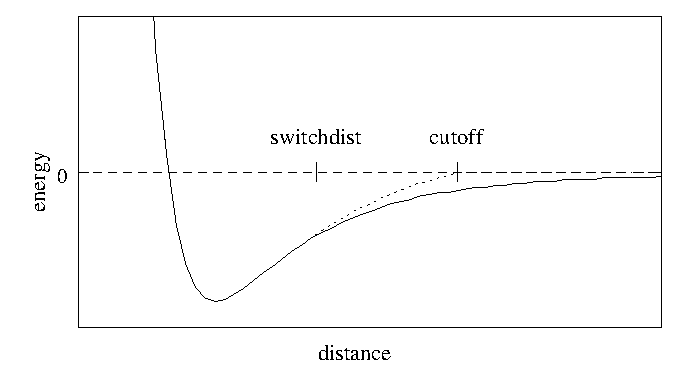
\includegraphics{figures/switching}}
  \caption[Graph of van der Waals potential with and without switching]
  {\small Graph of van der Waals potential with and without the
  application of the switching function.  With the switching function
  active, the potential is smoothly reduced to 0 at the cutoff distance.
  Without the switching function, there is a discontinuity where the
  potential is truncated.}
  \label{fig:switching}
\end{figure}

The switching function used is based on the X-PLOR switching
function.  The parameter {\tt switchdist} specifies the distance
at which the switching function should start taking effect to
bring the van der Waals potential to 0 smoothly at the cutoff distance.  
Thus, the value of {\tt switchdist} must always be less than that 
of {\tt cutoff}.


\subsubsection{Electrostatic interactions}
The handling of electrostatics is slightly
more complicated due to the incorporation of multiple timestepping for full
electrostatic interactions.  There are two cases to consider, one where
full electrostatics is employed and the other where electrostatics
are truncated at a given distance.
\prettypar
First let us consider the latter case, where electrostatics are truncated at
the cutoff distance.  Using this scheme, all electrostatic interactions
beyond a specified distance are ignored, or assumed to be zero.  If
{\tt switching} is set to {\tt on}, rather than having a discontinuity
in the potential
at the cutoff distance, a shifting function is applied to the electrostatic
potential as shown in Figure \ref{fig:shifting}.  As this figure shows, the
shifting function shifts the entire potential curve so that the curve
intersects the x-axis at the cutoff distance.  This shifting function
is based on the
shifting function used by X-PLOR.

\begin{figure}[htb]
  \center{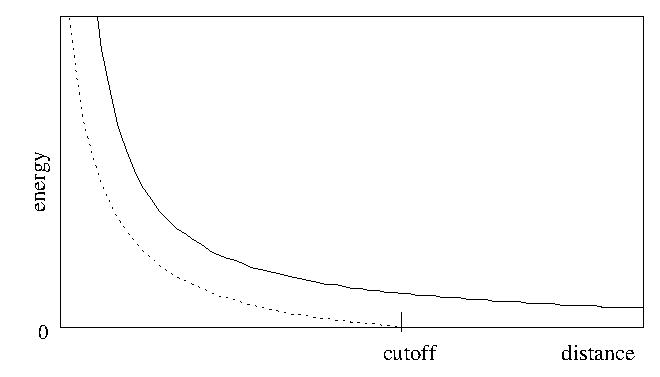
\includegraphics{figures/shifting}}
  \caption[Graph of electrostatic potential with and without shifting function]
  {\small Graph showing an electrostatic potential with and without the
  application of the shifting function.}
  \label{fig:shifting}
\end{figure}

Next, consider the case where full electrostatics are calculated.  In this
case, the electrostatic interactions are not truncated at any distance.  In
this scheme, the {\tt cutoff} parameter has a slightly different meaning
for the electrostatic interactions --- it represents
the {\it local interaction distance\/}, or distance within which electrostatic
pairs will be directly calculated every timestep.  Outside of this distance,
interactions will be calculated only periodically.  These forces
will be applied using a multiple timestep integration scheme as described in
Section \ref{section:mts}.

\begin{figure}[htb]
  \center{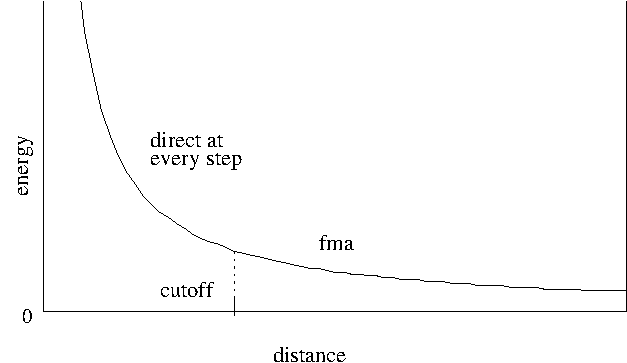
\includegraphics{figures/fmaOn}}
  \caption[Graph of electrostatic split between short and long range forces]
  {\small Graph showing an electrostatic potential 
  when full electrostatics are used within \NAMD, 
  with one curve portion calculated directly 
  and the other calculated using PME.}
  \label{fig:fmaOn}
\end{figure}



\subsubsection{Non-bonded force field parameters}

\begin{itemize}
%\item
%\NAMDCONF{eleccutoff}%
%{local interaction distance for electrostatic calculations (\AA)}%
%{positive decimal}%
%{Specifies the distance at which
%electrostatic interactions are truncated.
%If {\tt eleccutoff} is defined, it supersedes {\tt cutoff}.
%If {\tt eleccutoff} is not defined, then \verb }cutoff} {\em must}
%be defined.
%See Section \ref{section:electdesc} for a further discussion
%of this configuration value.}

%\item
%\NAMDCONF{vdwcutoff}%
%{local interaction distance for van der Waals calculations (\AA)}%
%{positive decimal}%
%{This value specifies the distance at which
%van der Waals interactions are truncated.
%If {\tt vdwcutoff} is defined, it supersedes {\tt cutoff}.
%If {\tt vdwcutoff} is not defined, then \verb }cutoff} {\em must}
%be defined.
%See Section \ref{section:electdesc} for a further discussion
%of this configuration value.}

\item
\NAMDCONF{cutoff}
{local interaction distance common to both electrostatic 
and van der Waals calculations (\AA)}
{positive decimal}
{%This value can substitute for either {\tt eleccutoff}
%or {\tt vdwcutoff} if either of those is undefined.
See Section \ref{section:electdesc} for more information.}

\item
\NAMDCONFWDEF{switching}{use switching function?}{{\tt on} or {\tt off}}
{{\tt on}}
{If {\tt switching} is
specified to be {\tt off}, then a truncated cutoff is performed.
If {\tt switching} is turned {\tt on}, then smoothing functions
are applied to both the electrostatics and van der Waals forces.
For a complete description of the non-bonded force parameters see
Section \ref{section:electdesc}.  If {\tt switching} is set to
{\tt on}, then {\tt switchdist} must also be defined.}

\item
\NAMDCONFWDEF{vdwForceSwitching}{use force switching for VDW?}{{\tt on} or {\tt off}}
{{\tt off}}
{If both {\tt switching} and {\tt vdwForceSwitching} are set to {\tt on},
then CHARMM force switching is used for van der Waals forces.
{\bf LJcorrection as implemented is inconsistent with vdwForceSwitching.}}

%\item
%\NAMDCONF{elecswitchdist}{distance at which to activate switching function for %electrostatic calculations (\AA)}{positive decimal $\leq$ {\tt eleccutoff}}
%{Distance at which the switching function
%used to smooth the truncation of
%electrostatic forces should begin to take effect.  
%This parameter only has meaning if {\tt switching} is 
%set to {\tt on}.  
%The value of {\tt elecswitchdist} must be less than
%or equal to the value of {\tt eleccutoff}, since the switching function
%is only applied on the range from {\tt elecswitchdist} to {\tt eleccutoff}.
%If {\tt elecswitchdist} is defined, it supersedes {\tt switchdist}.
%If {\tt elecswitchdist} is not defined and {\tt switching} is
%{\tt on}, then \verb }switchdist} {\em must} be defined.
%For a complete description of the non-bonded force parameters, see
%Section \ref{section:electdesc}.
%}

%\item
%\NAMDCONF{vdwswitchdist}%
%{distance at which to activate switching function 
%for van der Waals calculations (\AA)}%
%{positive decimal $\leq$ {\tt vdwcutoff}}%
%{Distance at which the switching function
%used to smooth the truncation of
%van der Waals forces should begin to take effect.  
%This parameter only has meaning if {\tt switching} is 
%set to {\tt on}.  
%The value of {\tt vdwswitchdist} must be less than
%or equal to the value of {\tt vdwcutoff}, since the switching function
%is only applied on the range from {\tt vdwswitchdist} to {\tt vdwcutoff}.
%If {\tt vdwswitchdist} is defined, it supersedes {\tt switchdist}.
%If {\tt vdwswitchdist} is not defined and {\tt switching} is
%{\tt on}, then \verb }switchdist} {\em must} be defined.
%For a complete description of the non-bonded force parameters, see
%Section \ref{section:electdesc}.
%}

\item
\NAMDCONF{switchdist}
{distance at which to activate switching/splitting function 
for electrostatic and van der Waals calculations (\AA)}
{positive decimal $\leq$ {\tt cutoff}}
{Distance at which the switching function
should begin to take effect.  
This parameter only has meaning if {\tt switching} is 
set to {\tt on}.  
The value of {\tt switchdist} must be less than
or equal to the value of {\tt cutoff}, since the switching function
is only applied on the range from {\tt switchdist} to {\tt cutoff}.  
For a complete description of the non-bonded force parameters see
Section \ref{section:electdesc}.}

\item
\NAMDCONF{exclude}
{non-bonded exclusion policy to use}
{{\tt none}, {\tt 1-2}, {\tt 1-3}, {\tt 1-4}, or {\tt scaled1-4}}
{\label{param:exclude}
%% This parameter is {\it required\/} for every simulation.
This parameter specifies which pairs of bonded atoms should
be excluded from non-bonded
interactions.  With the value of {\tt none}, no bonded pairs of atoms 
will be excluded.  With the value of {\tt 1-2}, all atom pairs that
are directly connected via a linear bond will be excluded.  With the
value of {\tt 1-3}, all {\tt 1-2} pairs will be excluded along with
all pairs of atoms that are bonded to a common
third atom (i.e., if atom A is bonded to atom B and atom B is bonded
to atom C, then the atom pair A-C would be excluded).
With the value of {\tt 1-4}, all {\tt 1-3} pairs will be excluded along
with all pairs connected by a set of two bonds (i.e., if atom A is bonded
to atom B, and atom B is bonded to atom C, and atom C is bonded to
atom D, then the atom pair A-D would be excluded).  With the value
of {\tt scaled1-4}, all {\tt 1-3} pairs are excluded and all pairs
that match the {\tt 1-4} criteria are modified.  The electrostatic
interactions for such pairs are modified by the constant factor
defined by {\tt 1-4scaling}.  
The van der Waals interactions are modified
by using the special 1-4 parameters defined in the parameter files.
The value of {\tt scaled1-4} is necessary to enable the modified
1-4 VDW parameters present in the CHARMM parameter files.
}

\item
\NAMDCONFWDEF{1-4scaling}{scaling factor for 1-4 electrostatic interactions}
{0 $\leq$ decimal $\leq$ 1}{1.0}
{Scaling factor for 1-4 electrostatic interactions.
This factor is only used when the
{\tt exclude} parameter is set to {\tt scaled1-4}.  In this case, this
factor is used to modify the electrostatic interactions between 1-4 atom
pairs.  If the {\tt exclude} parameter is set to anything but 
{\tt scaled1-4}, this parameter has no effect regardless of its value.}

\item
\NAMDCONFWDEF{dielectric}{dielectric constant for system}
{decimal $\geq$ 1.0}{1.0}
{Dielectric constant for the system.  A value of 1.0 implies no modification
of the electrostatic interactions.  Any larger value will lessen the
electrostatic forces acting in the system.}

\item
\NAMDCONFWDEF{nonbondedScaling}{scaling factor for nonbonded forces}
{decimal $\geq$ 0.0}{1.0}
{Scaling factor for electrostatic and van der Waals forces.
A value of 1.0 implies no modification of the interactions.
Any smaller value will lessen the
nonbonded forces acting in the system.}

\item
\NAMDCONFWDEF{vdwGeometricSigma}{use geometric mean to combine L-J sigmas}
{{\tt yes} or {\tt no}}{{\tt no}}
{Use geometric mean, as required by \index{OPLS} OPLS, rather than
traditional arithmetic mean when combining Lennard-Jones sigma parameters
for different atom types.}

\item
\NAMDCONFWDEF{limitdist}
{maximum distance between pairs for limiting interaction strength(\AA)}
{non-negative decimal}
{{\tt 0.}}
{
The electrostatic and van der Waals potential functions diverge
as the distance between two atoms approaches zero.
The potential for atoms closer than {\tt limitdist} is instead
treated as $a r^2 + c$ with parameters chosen to match the
force and potential at {\tt limitdist}.
This option should primarily be useful for alchemical free energy
perturbation calculations, since it makes the process of creating
and destroying atoms far less drastic energetically.
The larger the value of {\tt limitdist} the more the maximum force
between atoms will be reduced.
In order to not alter the other interactions in the simulation,
{\tt limitdist} should be less than the closest approach
of any non-bonded pair of atoms; 1.3\,\AA\ appears to satisfy this
for typical simulations but the user is encouraged to experiment.
There should be no performance impact from enabling this feature.
}

\item
\NAMDCONFWDEF{LJcorrection}
{Apply long-range corrections to the system energy and virial to
account for neglected vdW forces?}{{\tt yes} or {\tt no}}{{\tt no}}
{Apply an analytical correction to the reported vdW energy and virial
that is equal to the amount lost due to switching and cutoff of the LJ
potential. The correction will use the average of vdW parameters for
all particles in the system and assume a constant, homogeneous
distribution of particles beyond the switching distance. See 
\cite{Shirts2007} for details (the equations used in the NAMD
implementation are slightly different due to the use of a different
switching function). Periodic boundary conditions are required to make
use of tail corrections.
{\bf LJcorrection as implemented is inconsistent with vdwForceSwitching.}}

\end{itemize}


\subsubsection{PME parameters}

PME stands for Particle Mesh Ewald and is an efficient
full electrostatics method for use with periodic boundary conditions.
None of the parameters should affect energy conservation, although they may affect the accuracy of the results and momentum conservation.

\begin{itemize}

\item
\NAMDCONFWDEF{PME}{Use particle mesh Ewald for electrostatics?}{{\tt yes} or {\tt no}}{{\tt no}}
{Turns on particle mesh Ewald.}

\item
\NAMDCONFWDEF{PMETolerance}{PME direct space tolerance}{positive decimal}{$10^{-6}$}
{Affects the value of the Ewald coefficient and the overall accuracy of the results.}

\item
\NAMDCONFWDEF{PMEInterpOrder}{PME interpolation order}{positive integer}{4 (cubic)}
{Charges are interpolated onto the grid and forces are interpolated off using this many points, equal to the order of the interpolation function plus one.}

\item
\NAMDCONF{PMEGridSpacing}{maximum space between grid points}{positive real}
{The grid spacing partially determines the accuracy and efficiency of PME.
If any of the grid sizes below are not set, then PMEGridSpacing must be set
(recommended value is 1.0 \AA ) and will be used to calculate them.
If a grid size is set, then the grid spacing must be
at least PMEGridSpacing (if set, or a very large default of 1.5).}

\item
\NAMDCONF{PMEGridSizeX}{number of grid points in x dimension}{positive integer}
{The grid size partially determines the accuracy and efficiency of PME.
For speed, {\tt PMEGridSizeX} should have only small integer factors (2, 3 and 5).}

\item
\NAMDCONF{PMEGridSizeY}{number of grid points in y dimension}{positive integer}
{The grid size partially determines the accuracy and efficiency of PME.
For speed, {\tt PMEGridSizeY} should have only small integer factors (2, 3 and 5).}

\item
\NAMDCONF{PMEGridSizeZ}{number of grid points in z dimension}{positive integer}
{The grid size partially determines the accuracy and efficiency of PME.
For speed, {\tt PMEGridSizeZ} should have only small integer factors (2, 3 and 5).}

\item
\NAMDCONFWDEF{PMEProcessors}{processors for FFT and reciprocal sum}{positive integer}{larger of x and y grid sizes up to all available processors}
{For best performance on some systems and machines, it may be necessary to
restrict the amount of parallelism used.  Experiment with this parameter if
your parallel performance is poor when PME is used.}

\item
\NAMDCONFWDEF{FFTWEstimate}{Use estimates to optimize FFT?}{{\tt yes} or {\tt no}}{{\tt no}}
{Do not optimize FFT based on measurements, but on FFTW rules of thumb.
This reduces startup time, but may affect performance.}

\item
\NAMDCONFWDEF{FFTWUseWisdom}{Use FFTW wisdom archive file?}{{\tt yes} or {\tt no}}{{\tt yes}}
{Try to reduce startup time when possible by reading FFTW ``wisdom'' from a file, and saving wisdom generated by performance measurements to the same file for future use.
This will reduce startup time when running the same size PME grid on the same number of processors as a previous run using the same file.}

\item
\NAMDCONFWDEF{FFTWWisdomFile}{name of file for FFTW wisdom archive}{file name}{FFTW\_NAMD\_{\em version}\_{\em platform}.txt}
{File where FFTW wisdom is read and saved.
If you only run on one platform this may be useful to reduce startup times for all runs.
The default is likely sufficient, as it is version and platform specific.}

\end{itemize}

\subsubsection{Full direct parameters}

The direct computation of electrostatics 
is not intended to be used during 
real calculations, but rather as a testing or 
comparison measure.  Because of the ${\mathcal O}(N^2)$ 
computational complexity for performing 
direct calculations, this is {\it much} 
slower than using PME to compute full 
electrostatics for large systems.
In the case of periodic boundary conditions,
the nearest image convention is used rather than a
full Ewald sum.

\begin{itemize}

\item
\NAMDCONFWDEF{FullDirect}{calculate full electrostatics directly?}{{\tt yes} or {\tt no}}{{\tt no}}
{Specifies whether or not direct computation of 
full electrostatics should be performed.}

\end{itemize}


\subsubsection{Tabulated nonbonded interaction parameters}

In order to support coarse grained models and semiconductor force fields,
the tabulated energies feature replaces the normal van der Waals potential
for specified pairs of atom types with one interpolated from user-supplied
energy tables.  The electrostatic potential is not altered.

Pairs of atom types to which the modified interactions apply are specified
in a CHARMM parameter file by an {\tt NBTABLE} section consisting of lines
with two atom types and a corresponding interaction type name.
For example, tabulated interactions for SI-O, O-O, and SI-SI pairs would
be specified in a parameter file as:
\begin{verbatim}
NBTABLE
SI O SIO
O O OO
SI SI SISI
\end{verbatim}

Each interaction type must correspond to an entry in the energy table file.
The table file consists of a header formatted as:
\begin{verbatim}
# multiple comment lines
<number_of_tables> <table_spacing (A)> <maximum_distance (A)>
\end{verbatim}
followed by {\em number\_of\_tables} energy tables formatted as:
\begin{verbatim}
TYPE <interaction type name>
0 <energy (kcal/mol)> <force (kcal/mol/A)>
<table_spacing> <energy (kcal/mol)> <force (kcal/mol/A)>
<2*table_spacing> <energy (kcal/mol)> <force (kcal/mol/A)>
<3*table_spacing> <energy (kcal/mol)> <force (kcal/mol/A)>
...
<maximum_distance - 3*table_spacing> <energy (kcal/mol)> <force (kcal/mol/A)>
<maximum_distance - 2*table_spacing> <energy (kcal/mol)> <force (kcal/mol/A)>
<maximum_distance - table_spacing> <energy (kcal/mol)> <force (kcal/mol/A)>
\end{verbatim}

The table entry at {\em maximum\_distance} will match the energy of the
previous entry but have a force of zero.  The maximum distance must be at
least equal to the nonbonded cutoff distance and entries beyond the cutoff
distance will be ignored.  For the above example with a cutoff of 12 \AA\
the table file could look like:
\begin{verbatim}
# parameters for silicon dioxide
3 0.01 14.0
TYPE SIO
0 5.092449e+26 3.055469e+31
0.01 5.092449e+14 3.055469e+17
0.02 7.956951e+12 2.387085e+15
0.03 6.985526e+11 1.397105e+14
...
13.98 0.000000e+00 -0.000000e+00
13.99 0.000000e+00 -0.000000e+00
TYPE OO
0 1.832907e+27 1.099744e+32
0.01 1.832907e+15 1.099744e+18
0.02 2.863917e+13 8.591751e+15
0.03 2.514276e+12 5.028551e+14
...
13.98 0.000000e+00 -0.000000e+00
13.99 0.000000e+00 -0.000000e+00
TYPE SISI
0 0.000000e+00 -0.000000e+00
0.01 0.000000e+00 -0.000000e+00
...
13.98 0.000000e+00 -0.000000e+00
13.99 0.000000e+00 -0.000000e+00
\end{verbatim}

The following three parameters are required for tabulated energies.

\begin{itemize}

\item
\NAMDCONFWDEF{tabulatedEnergies}{use tabulated energies}{{\tt yes} or {\tt no}}{{\tt no}}
{Specifies whether or not tabulated energies will be used for
van der Waals interactions between specified pairs of atom types.}

\item
\NAMDCONF{tabulatedEnergiesFile}{file containing energy table}{file name}
{Provides one energy table for each interaction type in parameter file.
See format above.}

\item
\NAMDCONF{tableInterpType}{cubic or linear interpolation}{{\tt cubic} or {\tt linear}}
{Specifies the order for interpolating between energy table entries.}

\end{itemize}


\subsection{Water Models}
\label{section:water_models}

\NAMD~currently supports the 3-site TIP3P water model, 
the 4-site TIP4P water model,
and the 5-site SWM4-NDP water model 
(from the Drude force field)~\cite{Lamoureux-2006a}.  
TIP3P is the current default water model.  
Usage of alternative water models is described below. 

\begin{itemize}

  \item
    \NAMDCONFWDEF{waterModel}{using which water model?}{%
{\tt tip3}, {\tt tip4}, {\tt swm4}}{ {\tt tip3}}
    {Specifies the water model to be used.
When using the TIP3P water model, the ordering of atoms within each
TIP3P water molecule must be oxygen, hydrogen, hydrogen.  
When using the TIP4P water model, the ordering of atoms within each
TIP4P water molecule must be oxygen, hydrogen, hydrogen, lone pair.
When using the SWM4-NDP water model, 
the ordering of atoms within each SWM4-NDP water molecule
must be oxygen, Drude particle, lone pair, hydrogen, hydrogen.  
Alternative orderings will fail. } 

\end{itemize}


\subsection{Drude polarizable force field}
\label{section:drude_forcefield}

The Drude oscillator model represents induced electronic polarization 
by introducing an auxiliary particle attached to each polarizable 
atom via a harmonic spring.  The advantage with the Drude model is 
that it preserves the simple particle-particle Coulomb electrostatic 
interaction employed in nonpolarizable force fields, 
thus its implementation in \NAMD\ is more straightforward than 
alternative models for polarization.  
\NAMD\ performs the integration of Drude oscillators 
by employing a novel dual Langevin thermostat to freeze the Drude 
oscillators while maintaining the warm degrees of freedom 
at the desired temperature~\cite{JIAN2011}.  
Use of the Langevin thermostat enables better parallel scalability 
than the earlier reported implementation which made use of 
a dual Nos\'e-Hoover thermostat acting on, and within,
each nucleus-Drude pair~\cite{Lamoureux-2003a}.  
Performance results 
show that the \NAMD\ implementation of the Drude model maintains good 
parallel scalability, 
with an increase in computational cost by not more than twice 
that of using a nonpolarizable force field~\cite{JIAN2011}.  

The Drude polarizable force field requires some extensions to the
CHARMM force field.  
The Drude oscillators differ from typical spring bonds only in that they 
have an equilibrium length of zero.  
The Drude oscillators are optionally supplemented by a maximal 
bond length parameter, beyond which a quartic restraining potential 
is also applied.  
The force field is also extended by an anisotropic spring term 
that accounts for out-of-plane forces from a polarized atom and its 
covalently bonded neighbor with two more covalently bonded 
neighbors (similar in structure to an improper bond).  
The screened Coulomb correction of Thole is calculated between 
pairs of Drude oscillators that would otherwise be excluded from 
nonbonded interaction and 
optionally between non-excluded, nonbonded pairs of Drude oscillators 
that are within a prescribed cutoff distance~\cite{Thole81,van1998molecular}.  

Also included in the Drude force field 
are the use of off-centered massless interaction sites, 
so called ``lone pairs'' (LPs),
to avoid the limitations 
of centrosymmetric-based Coulomb interactions~\cite{Harder2006}.  
The coordinate of each LP site is constructed based on three ``guide'' atoms.
The calculated forces on the massless LP must be transferred 
to the guide atoms, 
preserving total force and torque.  
After an integration step of velocities and positions, 
the position of the LP is updated based on the three guide atoms, 
along with additional geometry parameters that give displacement 
and in-plane and out-of-plane angles.  
See our research web page
({\tt http://www.ks.uiuc.edu/Research/Drude/})
for additional details and parallel performance results.  


\subsubsection{Required input files}

No additional files are required by \NAMD\ to use the 
Drude polarizable force field.  
However, it is presently beyond the capability of 
the Psfgen tool to generate the PSF file needed to perform 
a simulation using the Drude model.  
For now, CHARMM is needed to generate correct input files.  

The CHARMM force field parameter files
specific to the Drude model are required.  
The PDB file must also include 
the Drude particles (mass between 0.1 and 1.0) 
and the LPs (mass 0).  
The Drude particles always immediately follow their parent atom.  
The PSF file augments the ``atom'' section with 
additional columns that include the 
``Thole'' and ``alpha'' parameters for the screened Coulomb 
interactions of Thole.  
The PSF file also requires additional sections that 
list the LPs, including their guide atoms and geometry parameters, 
and list the anisotropic interaction terms, including their parameters.  
A Drude-compatible PSF file is denoted by the 
keyword ``DRUDE'' given along the top line.  


\subsubsection{Standard output}

The \NAMD\ logging to standard output is extended to provide additional 
temperature data on the cold and warm degrees of freedom.  
Four additional quantities are listed 
on the {\tt ETITLE} and {\tt ENERGY} lines:
\begin{description}
\item[{\tt DRUDECOM}] gives the temperature for the warm center-of-mass 
degrees of freedom,
\item[{\tt DRUDEBOND}] gives the temperature for the cold Drude oscillator 
degrees of freedom,
\item[{\tt DRCOMAVG}] gives the average temperature 
(averaged since the previously reported temperature) 
for the warm center-of-mass degrees of freedom, 
\item[{\tt DRBONDAVG}] gives the average temperature 
(averaged since the previously reported temperature) 
for the cold Drude oscillator degrees of freedom.
\end{description}
The energies resulting from the Drude oscillators and the 
anisotropic interactions are summed into the {\tt BOND} energy.  
The energies resulting from the LPs and the screened Coulomb 
interactions of Thole are summed into the {\tt ELECT} energy.  


\subsubsection{Drude force field parameters}

The Drude model should be used with the Langevin thermostat enabled
({\tt Langevin=on}).  
Doing so permits the use of normal sized time steps (e.g., 1 fs).  
The Drude model is also compatible with constant pressure simulation 
using the Langevin piston.  
Long-range electrostatics may be calculated using PME.  
The nonbonded exclusions should generally be set to use either the
1-3 exclusion policy ({\tt exclude=1-3})
or the scaled 1-4 exclusion policy ({\tt exclude=scaled1-4}).  

The Drude water model (SWM4-NDP) is a 5-site model
with four charge sites and 
a negatively charged Drude particle~\cite{Lamoureux-2006a}, 
with the particles ordered in the input files as 
oxygen, Drude particle, LP, hydrogen, hydrogen.  
The atoms in the water molecules should be 
constrained ({\tt rigidBonds=water}),
with use of the SETTLE algorithm recommended ({\tt useSettle=on}).  
Explicitly setting the water model ({\tt waterModel=swm4}) is optional.  

\begin{itemize}

\item\NAMDCONFWDEF{drude}
{Perform integration of Drude oscillators?}
{{\tt on} or {\tt off}}
{{\tt off}}
{The integration uses a dual Langevin thermostat to freeze the Drude 
oscillators while maintaining the warm degrees of freedom at the
desired temperature.  Must also enable the Langevin thermostat.
If {\tt drude} is set to {\tt on}, then {\tt drudeTemp} must also be defined.}

\item\NAMDCONF{drudeTemp}
{temperature for freezing the Drude oscillators (K)}
{non-negative decimal}
{For stability, the Drude oscillators must be kept at a very cold termpature.
Using a Langevin thermostat, it is possible to set this temperature to 0 K.}

\item\NAMDCONF{drudeDamping}
{damping coefficient for Drude oscillators (1/ps)}
{positive decimal}
{The Langevin coupling coefficient to be applied to the Drude oscillators.  
If not given, {\tt drudeDamping} is set to the value of {\tt langevinDamping}.}

\item\NAMDCONF{drudeBondLen}
{Drude oscillator bond length, beyond which to apply restraint (\AA)}
{positive decimal}
{An additional quartic restraining potential is applied to a Drude 
oscillator if its length exceeds {\tt drudeBondLen}.  
The recommended value is 0.2 \AA, fitted from QM calculations.}

\item\NAMDCONF{drudeBondConst}
{Drude oscillator restraining force constant}
{positive decimal}
{If {\tt drudeBondConst} is defined,
an additional quartic restraining potential is applied to a Drude 
oscillator if its length exceeds {\tt drudeBondLen}.
The recommended value is 40000, fitted from QM calculations.}

\item\NAMDCONF{drudeNbTholeCut}
{nonbonded Thole interaction radius (\AA)}
{positive decimal}
{If {\tt drudeNbTholeCut} is defined, 
the screened Coulomb correction of Thole is also calculated
for non-excluded, nonbonded pairs of Drude oscillators that are
within this radius of interaction.
The recommended value is 5.0 \AA\ for a high concentration ($> 1$ M) 
ionic solution, or otherwise leave it 0.}

\end{itemize}


\subsection{MARTINI Residue-Based Coarse-Grain Forcefield}
%\label{sec:martini}

The MARTINI forcefield for residue-based coarse-grain models allows simulation of several tens of atoms as only several large coarse-grained particles~\cite{MARR2004, MARR2007, MONT2008}.  In the MARTINI model, each protein residue is represented by a backbone bead and usually one or more sidechain beads.  

When preparing MARTINI simulations it is important to include only those
dihedrals specified by the forcefield.  Using the ``auto dihedrals'' or 
``regenerate dihedrals'' feature of psfgen will create dihedrals for all
possible sets of four bonded atoms.  This is incorrect for MARTINI and
will result in energy jumps because the dihedral potential function is
degenerate for the angles of 180 degrees allowed by cosine-based angles.

When using MARTINI the following configuration parameters should be set as indicated:

\begin{verbatim}
cosAngles on
martiniSwitching on
dielectric 15.0
PME off
\end{verbatim}

\begin{itemize}

\item
\NAMDCONFWDEF{cosAngles}{enable the MARTINI cosine-based angle potential function}{{\tt on} or {\tt off}}{{\tt off}}
{Specifies whether or not the MARTINI forcefield is being used, specifically cosine-based angle potential function.
The cosine-based potential will only be used for angles in CHARMM parameter files that specify the cos keyword.} 

\item
\NAMDCONFWDEF{martiniSwitching}{enable the MARTINI Lennard-Jones switching function?}{{\tt on} or {\tt off}}{{\tt off}}
{Specifies whether or not the MARTINI forcefield is being used, specifically the Lennard-Jones switching function.} 

\item
\NAMDCONF{martiniDielAllow}{Allow dielectrics != 15.0 for use with MARTINI}{{\tt on} or {\tt off}}{{\tt off}}
{Allows user to specify a {\tt dielectric} not equal to 15.0, ie a non-standard dielectric for MARTINI.}

\end{itemize}


\subsection{Constraints and Restraints}
%\label{section:config_add}

\subsubsection{Bond constraint parameters}
\label{section:rigidBonds}
\begin{itemize}
\item
\NAMDCONFWDEF{rigidBonds}{controls if and how ShakeH is used}{{\tt none},
{\tt water}, {\tt all}}{{\tt none}} 
{When {\tt water} is selected, the hydrogen-oxygen and hydrogen-hydrogen
distances in waters are constrained to the nominal length or angle given
in the parameter file, making the molecules completely rigid.
When {\tt rigidBonds} is {\tt all}, waters are made rigid as described above
and the bond between each hydrogen and the (one) atom to which
it is bonded is similarly constrained.
For the default case {\tt none}, no lengths are constrained.
}

\item
\NAMDCONFWDEF{rigidTolerance}{allowable bond-length error for ShakeH (\AA)}
{positive decimal}{1.0e-8}
{
The ShakeH algorithm is assumed to have converged when all constrained
bonds differ from the nominal bond length by less than this amount.
}

\item
\NAMDCONFWDEF{rigidIterations}{maximum ShakeH iterations}{positive integer}{100}
{
The maximum number of iterations ShakeH will perform before giving up
on constraining the bond lengths.  If the bond lengths do not
converge, a warning message is printed, and the atoms are left at the
final value achieved by ShakeH.  
Although the default value is 100, 
convergence is usually reached after fewer than 10 iterations.
}

\item
\NAMDCONFWDEF{rigidDieOnError}{maximum ShakeH iterations}{{\tt on} or {\tt off}}
{{\tt on}}
{
Exit and report an error if rigidTolerance is not achieved after rigidIterations.
}

\item
\NAMDCONFWDEF{useSettle}{Use SETTLE for waters.}{{\tt on} or {\tt off}}
{{\tt on}}
{
If rigidBonds are enabled then use the non-iterative SETTLE algorithm to
keep waters rigid rather than the slower SHAKE algorithm.
}
\end{itemize}

\subsubsection{Harmonic restraint parameters}

The following describes the parameters for the 
harmonic restraints feature of \NAMD.
%Actually, this feature 
%should be referred to as harmonic restraints rather than 
%constraints, but
For historical reasons the terminology of 
``harmonic constraints'' has been carried over from X-PLOR.  
This feature allows a harmonic restraining force to be applied 
to any set of atoms in the simulation.

\begin{itemize}

\item
\NAMDCONFWDEF{constraints}{are constraints active?}{{\tt on} or {\tt off}}{{\tt off}}
{Specifies whether or not harmonic constraints are active.  If it 
is set to {\tt off}, then no harmonic constraints are computed.  
If it is set to {\tt on}, then 
harmonic constraints are calculated using the values specified 
by the parameters {\tt consref}, {\tt conskfile}, {\tt conskcol}, 
and {\tt consexp}.}

\item
\NAMDCONFWDEF{consexp}{exponent for harmonic constraint energy function}{positive, even integer}{2}
{Exponent to be use in the harmonic constraint energy function.  
This value must be a positive integer, and only even values really make 
sense.  This parameter is used only if {\tt constraints} is set to 
{\tt on}.}

\item
\NAMDCONF{consref}{PDB file containing constraint reference positions}{UNIX file name}
{PDB file to use for reference positions for harmonic constraints.  
Each atom that has an active constraint will be constrained about 
the position specified in this file.}

\item
\NAMDCONF{conskfile}{PDB file containing force constant values}{UNIX filename}
{PDB file to use for force constants for 
harmonic constraints.}

\item
\NAMDCONF{conskcol}{column of PDB file containing force constant}{{\tt X}, {\tt Y}, {\tt Z}, {\tt O}, or {\tt B}}
{Column of the PDB file to use for the harmonic constraint force constant.
This parameter may specify any of the floating point fields of the PDB file, 
either X, Y, Z, occupancy, or beta-coupling (temperature-coupling).  
Regardless of which column is used, a value of 0 indicates that the atom 
should not be constrained.  
Otherwise, the value specified is used as the force constant for 
that atom's restraining potential.}

\item
\NAMDCONFWDEF{constraintScaling}{scaling factor for harmonic constraint energy function}{positive}{1.0}
{The harmonic constraint energy function is multiplied by this parameter,
making it possible to gradually turn off constraints during equilibration.
This parameter is used only if {\tt constraints} is set to 
{\tt on}.}

\item
\NAMDCONFWDEF{selectConstraints}{Restrain only selected Cartesian components of the coordinates?}{{\tt on} or {\tt off}}{{\tt off}}
{This option is useful to restrain the positions of atoms to a plane or a line in space. If active,
 this option will ensure that only selected Cartesian components of the coordinates are restrained.
 E.g.: Restraining the positions of atoms to their current z values with no restraints
 in x and y will allow the atoms to move in the x-y plane while retaining their original z-coordinate.
 Restraining the x and y values will lead to free motion only along the z coordinate.}

\item
\NAMDCONFWDEF{selectConstrX}{Restrain X components of coordinates}{{\tt on} or {\tt off}}{{\tt off}}
{Restrain the Cartesian x components of the positions.}
\item
\NAMDCONFWDEF{selectConstrY}{Restrain Y components of coordinates}{{\tt on} or {\tt off}}{{\tt off}}
{Restrain the Cartesian y components of the positions.}
\item
\NAMDCONFWDEF{selectConstrZ}{Restrain Z components of coordinates}{{\tt on} or {\tt off}}{{\tt off}}
{Restrain the Cartesian z components of the positions.}

\end{itemize}

\subsubsection{Fixed atoms parameters}

Atoms may be held fixed during a simulation.  \NAMD\ avoids calculating most interactions in which all affected atoms are fixed unless {\tt fixedAtomsForces} is specified.

\begin{itemize}

\item
\NAMDCONFWDEF{fixedAtoms}{are there fixed atoms?}{{\tt on} or {\tt off}}{{\tt off}}
{Specifies whether or not fixed atoms are present.} 

\item
\NAMDCONFWDEF{fixedAtomsForces}{are forces between fixed atoms calculated?}{{\tt on} or {\tt off}}{{\tt off}}
{Specifies whether or not forces between fixed atoms are calculated.  This option is required to turn fixed atoms off in the middle of a simulation.
These forces will affect the pressure calculation, and you should leave this option off when using constant pressure if the coordinates of the fixed atoms have not been minimized.
The use of constant pressure with significant numbers of fixed atoms is not recommended.}

\item
\NAMDCONFWDEF{fixedAtomsFile}{PDB file containing fixed atom parameters}
{UNIX filename}{{\tt coordinates}}
{PDB file to use for the fixed atom flags for each atom.  
If this parameter is not specified, then 
the PDB file specified by {\tt coordinates} is used.}

\item
\NAMDCONFWDEF{fixedAtomsCol}{column of PDB containing fixed atom parameters}
{{\tt X}, {\tt Y}, {\tt Z}, {\tt O}, or {\tt B}}{{\tt O}} 
{Column of the PDB file to use for the containing fixed atom parameters for 
each atom.  The coefficients can be read from any 
floating point column of the PDB file.  
A value of 0 indicates that the atom is not fixed.}

\end{itemize}

\subsubsection{Extra bond, angle, and dihedral restraints}

Additional bond, angle, and dihedral energy terms may be applied to system,
allowing secondary or tertiary structure to be restrained, for example.
Extra bonded terms are not considered part of the molecular structure
and hence do not alter nonbonded exclusions.
The energies from extra bonded terms are included with the normal
bond, angle, and dihedral energies in \NAMD\ output.

All extra bonded terms are harmonic potentials of the form
$U(x) = k (x-x_{ref})^2$ except dihedrals and impropers with
a non-zero periodicity specified, which use
$U(x) = k (1 + cos(n x - x_{ref}))$.
The only difference between dihedrals and
impropers is the output field that their potential energy is added to.

The extra bonded term implementation shares the parallel implementation
of regular bonded terms in \NAMD, allowing large numbers of extra terms
to be specified with minimal impact on parallel scalability.
Extra bonded terms do not have to duplicate normal bonds/angles/dihedrals,
but each extra bond/angle/dihedral should only involve nearby atoms.
If the atoms involved are too far apart a bad global bond count will be
reported in parallel runs.

Extra bonded terms are enabled via the following options:

\begin{itemize}

\item
\NAMDCONFWDEF{extraBonds}{enable extra bonded terms?}{{\tt on} or {\tt off}}{{\tt off}}
{Specifies whether or not extra bonded terms are present.} 

\item
\NAMDCONF{extraBondsFile}{file containing extra bonded terms}{file}
{File containing extra bonded terms.  May be repeated for multiple files.} 

\end{itemize}

The extra bonds file(s) should contain lines of the following formats:

\begin{itemize}
\item
{\tt bond <atom> <atom> <k> <ref>}
\item
{\tt angle <atom> <atom> <atom> <k> <ref>}
\item
{\tt dihedral <atom> <atom> <atom> <atom> <k> <ref>}
\item
{\tt dihedral <atom> <atom> <atom> <atom> <k> <n> <ref>}
\item
{\tt improper <atom> <atom> <atom> <atom> <k> <ref>}
\item
{\tt improper <atom> <atom> <atom> <atom> <k> <n> <ref>}
\item
{\tt \# <comment ...>}
\end{itemize}

In all cases {\tt <atom>} is a {\bf zero-based} atom index
(the first atom has index 0),
{\tt <ref>} is a reference distance in \AA\ (bond) or angle in degrees (others),
and {\tt <k>} is a spring constant in the potential energy function
$U(x) = k (x-x_{ref})^2$ or, for dihedrals and impropers with 
periodicity {\tt <n>} specified and not 0, $U(x) = k (1 + cos(n x - x_{ref}))$.
Note that $x_{ref}$ is only a minimum for the harmonic potential;
the sinusoidal potential has minima at $(x_{ref} + 180)/n + i \times 360/n$.




% Implicit Solvent Parameters
\newpage
\begin{comment}
\documentclass[11pt]{article}
\usepackage{graphicx}
\usepackage{makeidx}
\usepackage{amssymb}
\usepackage{amsmath}
\usepackage[stable]{footmisc}

\newcommand{\NAMDCONFWDEF}[5]{%
%  \addcontentsline{toc}{subparagraph}{#1}%
  {\bf \tt #1 } $<$ #2 $>$ \index{#1 parameter} \\%
  {\bf Acceptable Values: } #3 \\%
  {\bf Default Value: } #4 \\%
  {\bf Description: } #5%
}


\begin{document}
\end{comment}

\section{Generalized Born Implicit Solvent}
\label{section:gbis}

Generalized Born implicit solvent (GBIS) is a fast but approximate method for calculating molecular electrostatics in solvent as described by the Poisson Boltzmann equation which models water as a dielectric continuum.
GBIS enables the simulation of atomic structures without including explicit solvent water.
The elimination of explicit solvent greatly accelerates simulations;
this speedup is lessed by the increased computational complexity of the implicit solvent electrostatic calculation and a longer interaction cutoff.
These are discussed in greater detail below.


%\subsection{Theoretical Background}
\subsection{Theoretical Background}
Water has many biologically necessary properties, one of which is as a dielectric.
As a dielectric, water screens (lessens) electrostatic interactions between charged particles. 
Water can therefore be crudely modeled as a dielectric continuum.
In this manner, the electrostatic forces of a biological system can be expressed as a system of differential equations which can be solved for the electric field caused by a collection of charges.


%\subsubsection{Poisson Boltzmann Equation}
\subsubsection{Poisson Boltzmann Equation}
The Poisson Boltzmann equation (PBE),
$$
\vec{\nabla} \cdot \left[ \epsilon (\vec{r}) \vec{\nabla} \Psi(\vec{r})  \right] = -4\pi \rho^f (\vec{r}) - 4 \pi \sum_i c_i^\infty q_i \lambda(\vec{r}) \cdot \exp \left[ \frac{-q_i \Psi(\vec{r})}{k_B T} \right]
$$
is a nonlinear equation which solves for the electrostatic field, $\Psi(\vec{r})$, based on
the position dependent dielectric, $\epsilon(\vec{r})$,
the position-dependent accessibility of position $\vec{r}$ to the ions in solution, $\lambda(\vec{r})$,
the solute charge distribution, $\rho^f(\vec{r})$,
and the bulk charge density, $c_i^\infty$, of ion $q_i$.
While this equation does exactly solve for the electrostic field of a charge distribution in a dielectric, it is very expensive to solve, and therefore not suitable for molecular dynamics.


%\subsubsection{Generalized Born}
\subsubsection{Generalized Born}
The Generalized Born (GB) equation is an approximation of the PBE.
It models atoms as charged spheres whose internal dielectric is lower than that of the environment.
The screening which each atom, $i$, experiences is determined by the local environment;
the more atom $i$ is surrounded by other atoms, the less it's electrostatics will be screened since it is more surrounded by low dielectric; this property is called one atom descreening another.
Different GB models calculate atomic descreening differently.
Descreening is used to calculate the Born radius, $\alpha_i$, of each atom.
The Born radius of an atom measures the degree of descreening.
A large Born radius represents small screening (strong electric field) as if the atom were in vacuum.
A small Born radius represents large screening (weak electric field) as if the atom were in bulk water.
The next section describes how the Born radius is calculated and how it is used to calculate electrostatics.

%\subsubsection{Generalized Born OBC}
\subsubsection{Generalized Born Equations}
In a GB simulation, the total electrostatic force on an atom, $i$, is the net Coulomb force on atom $i$ (from nearby atoms) minus the GB force on atom $i$ (also caused by nearby atoms):
$$
\vec{F}_i = \vec{F}_i^{Coulomb} - \vec{F}_i^{GB}.
$$
Forces are contributed by other nearby atoms within a cutoff.
The GB force on atom $i$ is the derivative of the total GB energy with respect to relative atom distances $r_{ij}$,
\begin{eqnarray}
\vec{F}_i^{GB}&=&-\sum_j \left[  \frac{d E_T^{GB}}{d r_{ij}}  \right]  \hat{r}_{ji} \\
&=&-\sum_j \left[  \sum_k \frac{\partial E_T^{GB}}{\partial \alpha_k}\frac{d \alpha_k}{d r_{ij}} + \frac{\partial E_{ij}^{GB}}{\partial r_{ij}}  \right]  \hat{r}_{ji} \\
&=&-\sum_j \left[  \frac{\partial E_T^{GB}}{\partial \alpha_i}\frac{d \alpha_i}{d r_{ij}}+\frac{\partial E_T^{GB}}{\partial \alpha_j}\frac{d \alpha_j}{d r_{ij}}+ \frac{\partial E_{ij}^{GB}}{\partial r_{ij}}  \right]  \hat{r}_{ji} \; .
\end{eqnarray}
where the partial derivatives are included since the Born radius, $\alpha$, is a function of all relative atom distances.
The total GB energy of the system is
\begin{equation}
E_T^{GB} = \sum_i \sum_{j>i} E_{ij}^{GB} + \sum_{i} E_{ii}^{GB} \; ,
\end{equation}
where $E_{ii}^{GB}$ is the Born radius dependent self energy of atom $i$, and the GB energy between atoms $i$ and $j$ is given by
\begin{equation}
E^{GB}_{ij} = - k_e D_{ij} \frac{q_i q_j}{f_{ij}} \; .
\end{equation}
The dielectric term~\cite{SRIN99} is
\begin{equation}
D_{ij} = \left( \frac{1}{\epsilon_p} - \frac{\exp{\left(-\kappa f_{ij}\right)}}{\epsilon_s} \right) \; ,
\end{equation}
and the GB function~\cite{STIL90} is
\begin{equation}
f_{ij} = \sqrt{r_{ij}^2 + \alpha_i \alpha_j \exp{\left(\frac{-r_{ij}^2}{4 \alpha_i \alpha_j}\right)}} \; .
\end{equation}
As the Born radii of atoms $i$ and $j$ decrease (increasing screening), the effective distance between the atoms ($f_{ij}$) increases.
The implicit solvent implemented in NAMD is the model of Onufriev, Bashford and Case~\cite{ONUF00, ONUF04} which calculates the Born radius as
\begin{equation}
\alpha_k = \left[ \frac{1}{\rho_{k0}} - \frac{1}{\rho_k}\textrm{tanh}\left(\delta\psi_k - \beta\psi_k^2 + \gamma\psi_k^3\right)\right]^{-1} 
\end{equation}
where
\begin{equation}
\psi_k = \rho_{k0} \sum_l H_{kl} \; .
\end{equation}
$H_{ij}$ is the piecewise descreening function~\cite{ONUF04,HAWK96,SCHA90}; the seven piecewise regimes are
\begin{equation}
\textrm{Regimes} = \left\{
\begin{array}{r l l}
\textrm{0} & r_{ij} > r_c + \rho_{js} &(\textrm{sphere}~j~\textrm{beyond cutoff})\\
\textrm{I} & r_{ij} > r_c - \rho_{js} &(\textrm{sphere}~j~\textrm{partially within cutoff}) \\
\textrm{II} & r_{ij} > 4\rho_{js} &(\textrm{artificial regime for smoothing})\\
\textrm{III} & r_{ij} > \rho_{i0} + \rho_{js} &(\textrm{spheres not overlapping})\\
\textrm{IV} & r_{ij} > \left| \rho_{i0} - \rho_{js} \right| &(\textrm{spheres overlapping}) \\
\textrm{V} & \rho_{i0} < \rho_{js} &(\textrm{sphere}~i~\textrm{inside~sphere}~j)\\
\textrm{VI} & \textrm{otherwise} &(\textrm{sphere}~j~\textrm{inside~sphere}~j)\\
\end{array}\right.
\end{equation}
and the values of $H_{ij}$ are
\begin{equation}
H_{ij} = \left\{
\begin{array}{r l}
\textrm{0} & 0 \\
\textrm{I} & \frac{1}{8 r_{ij}}\left[ 1 + \frac{2 r_{ij}}{r_{ij}-\rho_{js}} + \frac{1}{r_c^2}\left( r_{ij}^2-4 r_c r_{ij} - \rho_{js}^2\right) +2 \ln \frac{r_{ij}-\rho_{js}}{r_c}\right] \\
\textrm{II} & \frac{\rho_{js}^2}{r_{ij}^2} \frac{\rho_{js}}{r_{ij}^2} \left[ a+ \frac{\rho_{js}^2}{r_{ij}^2}\left( b+\frac{\rho_{js}^2}{r_{ij}^2}\left( c+\frac{\rho_{js}^2}{r_{ij}^2}\left( d+\frac{\rho_{js}^2}{r_{ij}^2} e \right) \right) \right) \right] \\
\textrm{III} & \frac{1}{2} \left[\frac{\rho_{js}}{r_{ij}^2-\rho_{js}^2} + \frac{1}{2 r_{ij}} \ln \frac{r_{ij}-\rho_{js}}{r_{ij}+\rho_{js}} \right]\\
\textrm{IV} & \frac{1}{4} \left[ \frac{1}{\rho_{i0}}\left( 2-\frac{1}{2r_{ij}\rho_{i0}}\left(r_{ij}^2+\rho_{i0}^2-\rho_{js}^2\right)\right) - \frac{1}{r_{ij}+\rho_{js}} + \frac{1}{r_{ij}} \ln \frac{\rho_{i0}}{r_{ij}+\rho_{js}} \right]\\
\textrm{V} & \frac{1}{2} \left[\frac{\rho_{js}}{r_{ij}^2-\rho_{js}^2} + \frac{2}{\rho_{i0}} + \frac{1}{2 r_{ij}} \ln \frac{\rho_{js}-r_{ij}}{r_{ij}+\rho_{js}} \right]\\
\textrm{VI} & 0
\end{array}
\right.
\end{equation}
Below are defined the derivatives of the above functions which are required for force calculations.
%dEij dr
\begin{equation}
\frac{\partial E_{ij}}{\partial r_{ij}} = - k_e \left[
\frac{q_i q_j}{f_{ij}} \frac{\partial D_{ij}}{\partial r_{ij}}  
 - 
 \frac{q_i q_j D_{ij}}{f_{ij}^2} \frac{\partial f_{ij}}{\partial r_{ij}}
\right]
\end{equation}
%d Dij
\begin{equation}
\frac{\partial D_{ij}}{\partial r_{ij}} = \frac{\kappa}{\epsilon_s} \exp{\left(-\kappa f_{ij}\right)\frac{\partial f_{ij}}{\partial r_{ij}}}
\end{equation}
%d f
\begin{equation}
\frac{\partial f_{ij}}{\partial r_{ij}} = \frac{r_{ij}}{f_{ij}} \left[1 - \frac{1}{4} \exp{\left(\frac{-r_{ij}^2}{4 \alpha_i \alpha_j}\right)} \right]
\end{equation}
%d alpha sum
\begin{equation}
\frac{d \alpha_k}{d r_{ij}} = \frac{\alpha_k^2}{\rho_k}\left(1-\textrm{tanh}^2\left(\delta \psi_k - \beta \psi_k^2 + \gamma \psi_k^3\right)\right)
\left( \delta - 2\beta\psi_k+3\beta\psi_k^2\right) \frac{d \psi_k}{d r_{ij}}
\end{equation}
%d psi
\begin{eqnarray}
\frac{d \psi_k}{d r_{ij}}
&=&\rho_{k0} \sum_l \frac{d H_{kl}}{d r_{ij}} \\
&=&\rho_{k0} \sum_l \frac{\partial H_{kl}}{\partial r_{kl}}\frac{d r_{kl}}{d r_{ij}}\\
&=&\rho_{k0} \left[ \frac{\partial H_{kj}}{\partial r_{kj}}\delta_{ki} + \frac{\partial H_{ki}}{\partial r_{ki}}\delta_{kj} \right]
\end{eqnarray}
%d alpha 
\begin{eqnarray}
\frac{d \alpha_k}{d r_{ij}} =
& \frac{\alpha_i^2\rho_{i0}}{\rho_i}\left(1-\textrm{tanh}^2\left(\delta \psi_i - \beta \psi_i^2 + \gamma \psi_i^3\right)\right)
\left( \delta - 2\beta\psi_i+3\beta\psi_i^2\right) \frac{\partial H_{ij}}{\partial r_{ij}} \delta_{ki}\nonumber \\
+ &
\frac{\alpha_j^2\rho_{j0}}{\rho_j}\left(1-\textrm{tanh}^2\left(\delta \psi_j - \beta \psi_j^2 + \gamma \psi_j^3\right)\right)
\left( \delta - 2\beta\psi_j+3\beta\psi_j^2\right) \frac{\partial H_{ji}}{\partial r_{ij}} \delta_{kj}
\end{eqnarray}
\begin{equation}
\frac{\partial E_{ij}}{\partial \alpha_i} = -\frac{1}{\alpha_i}\frac{k_e q_i q_j}{2 f_{ij}^2}\left( \frac{\kappa}{\epsilon_s}\exp{\left(-\kappa f_{ij}\right)} - \frac{D_{ij}}{f_{ij}}\right)
\left(\alpha_i\alpha_j + \frac{r_{ij}^2}{4}\right)\exp{\left(\frac{-r_{ij}^2}{4 \alpha_i \alpha_j}\right)}
\end{equation}
\begin{equation}
\frac{\partial E_{ij}}{\partial \alpha_j} = -\frac{1}{\alpha_j}\frac{k_e q_i q_j}{2 f_{ij}^2}\left( \frac{\kappa}{\epsilon_s}\exp{\left(-\kappa f_{ij}\right)} - \frac{D_{ij}}{f_{ij}}\right)
\left(\alpha_i\alpha_j + \frac{r_{ij}^2}{4}\right)\exp{\left(\frac{-r_{ij}^2}{4 \alpha_i \alpha_j}\right)}
\end{equation}
%d Hij
\begin{equation}
\frac{\partial H_{ij}}{\partial r_{ij}} = \left\{
\begin{array}{r l}
\textrm{0} & 0 \\
\textrm{I} &
\left[-\frac{\left(r_c+\rho_{js}-r_{ij}\right)\left(r_c-\rho_{js}+r_{ij}\right)\left(\rho_{js}^2+r_{ij}^2\right)}{8r_c^2r_{ij}^2\left(\rho_{js}-r_{ij}\right)^2}
-\frac{1}{4r_{ij}^2}\ln \frac{r_{ij}-\rho_{js}}{r_c}
\right] \\
\textrm{II} &
\left[
-4a\frac{\rho_{js}^3}{r_{ij}^5}
-6b\frac{\rho_{js}^5}{r_{ij}^7}
-8c\frac{\rho_{js}^7}{r_{ij}^9}
-10d\frac{\rho_{js}^9}{r_{ij}^{11}}
-12e\frac{\rho_{js}^{11}}{r_{ij}^{13}}
\right] \\
\textrm{III} &
\frac{1}{2}\left[
-\frac{\rho_{js}\left(r_{ij}^2+\rho_{js}^2\right)}{r_{ij}\left(r_{ij}^2-\rho_{js}^2\right)^2}
-\frac{1}{2r_{ij}^2} \ln \frac{r_{ij}-\rho_{js}}{r_{ij}+\rho_{js}}
\right] \\
\textrm{IV} &
\frac{1}{4} \left[
-\frac{1}{2\rho_{i0}^2}
+\frac{r_{ij}^2\left(\rho_{i0}^2-\rho_{js}^2\right)-2 r_{ij}\rho_{js}^3+\rho_{js}^2\left(\rho_{i0}^2-\rho_{js}^2\right)}{2r_{ij}^2\rho_{i0}^2\left(r_{ij}+\rho_{js}\right)^2}
-\frac{1}{r_{ij}^2}\ln\frac{\rho_{i0}}{r_{ij}+\rho_{js}}
\right] \\
\textrm{V} &
\frac{1}{2}\left[
-\frac{\rho_{js}\left(r_{ij}^2+\rho_{js}^2\right)}{r_{ij}\left(r_{ij}^2-\rho_{js}^2\right)^2}
-\frac{1}{2r_{ij}^2} \ln \frac{\rho_{js}-r_{ij}}{r_{ij}+\rho_{js}}
\right] \\
\textrm{VI} & 0
\end{array}
\right.
\end{equation}
Other variables referenced in the above GB equations are
\begin{list}{}
\item $r_{ij}$ - distance between atoms i and j; calculated from atom coordinates.
\item $\kappa$ - debye screening length; calculated from ion concentration, $\kappa^{-1} = \sqrt{\frac{\epsilon_0 \epsilon_p k T}{2 N_A e^2 I}}$; $\kappa^{-1} = 10$~\AA~for 0.1~M monovalent salt.
\item $\epsilon_s$ - dielectric constant of solvent.
\item $\epsilon_p$ - dielectric constant of protein.
\item $\alpha_i$ - Born radius of atom $i$.
\item $\rho_i$ - intrinsic radius of atom $i$ taken from Bondi~\cite{BOND64}.
\item $\rho_0$ - intrinsic radius offset; $\rho_0 = 0.09$~\AA~by default~\cite{ONUF04}.
\item $\rho_{i0} = \rho_i - \rho_0$
\item $\rho_{is} = \rho_{i0} S_{ij}$
\item $S_{ij}$ - atom radius scaling factor~\cite{HAWK96,SRIN99}.
\item $k_e$ - Coulomb's constant, $\frac{1}{4 \pi \epsilon_0}$, 332.063711 kcal~\AA~/ e$^2$.
\item $\{\delta, \beta, \gamma\} = \{0.8, 0, 2.91\}~\textrm{or}~\{1.0, 0.8, 4.85\}$~\cite{ONUF04}
\end{list}


%\subsubsection{3-Phase Calculation}
\subsection{3-Phase Calculation}

The GBIS algorithm requires three phases of calculation, with each phase containing an iteration over all atom pairs with the cutoff.
In phase 1, the screening of atom pairs is summed; at the conclusion of phase 1, the Born radii are calculated.
In phase 2, the $\frac{\partial E_{ij}^{GB}}{\partial r_{ij}}$ force contribution (hereafter called the dEdr force) is calculated as well as the partial derivative of the Born radii with respect to the atom positions, $\frac{d \alpha_i}{d r_{ij}}$.
In phase 3, the $\frac{\partial E_T^{GB}}{\partial \alpha_i}\frac{d \alpha_i}{d r_{ij}}$ force contribution (hereafter called the dEda force) is calculated.


%\subsubsection{Configuration Parameters}
\subsection{Configuration Parameters}

When using GBIS, user's should not use {\tt PME} (because it is not compatible with GBIS).
Periodic boundary conditions are supported but are optional.
User's will need to increase {\tt cutoff}; 16-18~\AA~is a good place to start but user's will have to check their system's behavior and increase {\tt cutoff} accordingly.
GBIS interactions are never excluded regardless of the type of force field used, thus user's can choose any value for {\tt exclude} without affecting GBIS; user's should still choose {\tt exclude} based on the force field as if using explicit solvent.
When using GBIS, multiple timestepping behaves as follows:
the dEdr force is calculated every {\tt nonbondedFreq} steps (as with explicit solvent, 2 is a reasonable frequency) and
the dEda force is calculated every {\tt fullElectFrequency} steps (because dEda varies more slowly than dEdr, 4 is a reasonable frequency).

%begin configuration parameter list
\begin{itemize}

\item
\NAMDCONFWDEF{GBIS}{Use Generalized Born Implicit Solvent?} {{\tt on} or {\tt off}} {{\tt off}} {Turns on GBIS method in NAMD. }

\item
\NAMDCONFWDEF{solventDielectric}{dielectric of water} {positive decimal} {78.5} {Defines the dielectric of the solvent, usually 78.5 or 80.}

\item
\NAMDCONFWDEF{intrinsicRadiusOffset}{shrink the intrinsic radius of atoms (\AA)} {positive decimal} {0.09} {This offset shrinks the intrinsic radius of atoms (used only for calculating Born radius) to give better agreement with Poisson Boltzmann calculations. Most users should not change this parameter.}

\item
\NAMDCONFWDEF{ionConcentration}{concentration of ions in solvent (Molar)} {positive decimal} {0.2} {An ion concentration of 0~M represents distilled water. Increasing the ion concentration increases the electrostatic screening.}

\item
\NAMDCONFWDEF{GBISDelta}{GB$^{OBC}$ parameter for calculating Born radii} {decimal} {1.0} {Use $\{{\tt GBISDelta}, {\tt GBISBeta},{\tt GBISGamma}\} = \{1.0, 0.8, 4.85\}$ for GB$^{OBC}$II and $\{0.8, 0.0, 2.90912\}$ for GB$^{OBC}$I. See $\{\alpha, \beta, \gamma\}$ in \cite{ONUF04} for more information.}

\item
\NAMDCONFWDEF{GBISBeta}{GB$^{OBC}$ parameter for calculating Born radii} {decimal} {0.8} {See {\tt GBISDelta}.}

\item
\NAMDCONFWDEF{GBISGamma}{GB$^{OBC}$ parameter for calculating Born radii} {decimal} {4.85} {See {\tt GBISDelta}.}

\item
\NAMDCONFWDEF{alphaCutoff}{cutoff used in calculating Born radius and derivatives (phases 1 and 3) (\AA)} {positive decimal} {15} {Cutoff used for calculating Born radius. Only atoms within this cutoff de-screen an atom. Though {\tt alphaCutoff} can bet set to be larger or shorter than {\tt cutoff}, since atom forces are more sensitive to changes in position than changes in Born radius, user's should generally set {\tt alphaCutoff} to be shorter than {\tt cutoff}.}

\item
\NAMDCONFWDEF{SASA}{whether or not to calculate SASA} {{\tt on} or {\tt off}} {{\tt off}} {The nonpolar / hydrophobic energy contribution from implicit solvent is calculated; it is proportional to the solvent-accessible surface area (SASA) which is calculated by the Linear Combination of Pairwise Overlap (LCPO) method~\cite{WEIS99}. It evaluated every {\tt nonbondedFreq} steps and its energy is added into the reported {\tt ELECT} energy.}

\item
\NAMDCONFWDEF{surfaceTension}{surface tension of SASA energy} {positive decimal} {0.005~kcal/mol/\AA$^2$} {Surface tension used when calculating hydrophobic {\tt SASA} energy; $E_{\rm nonpolar} = {\rm surfaceTension} \times {\rm surfaceArea}$.}

\end{itemize}

Below is a sample excerpt from a NAMD config file for nonbonded and multistep parameters when using {\tt GBIS} and {\tt SASA}:
\begin{verbatim}
#GBIS parameters
GBIS on
ionConcentration 0.3
alphaCutoff 14
#nonbonded parameters
switching on
switchdist 15
cutoff 16
pairlistdist 18
#hydrophobic energy
sasa on
surfaceTension 0.006
#multistep parameters
timestep 1
nonbondedFreq 2
fullElectFrequency 4
\end{verbatim}
%\bibliographystyle{unsrt}
%\bibliography{ug}
%\bibliography{../../LaTeX/Bibliography/data_base}

\begin{comment}
\end{document}
\end{comment}


% Standard minimization and dynamics parameters
\newpage
\section{Standard Minimization and Dynamics Parameters}
\label{section:dynamics}


\subsection{Boundary Conditions}

In addition to periodic boundary conditions, NAMD provides spherical and
cylindrical boundary potentials to contain atoms in a given volume.
To apply more general boundary potentials written in Tcl, use
{\tt tclBC} as described in Sec.~\ref{section:tclBC}.

\subsubsection{Periodic boundary conditions}

\NAMD\ provides periodic boundary conditions in 1, 2 or 3 dimensions.
The following parameters are used to define these boundary conditions.  

\begin{itemize}

\item
\NAMDCONFWDEF{cellBasisVector1}{basis vector for periodic boundaries (\AA)}{vector}{0 0 0}
{Specifies a basis vector for periodic boundary conditions.}

\item
\NAMDCONFWDEF{cellBasisVector2}{basis vector for periodic boundaries (\AA)}{vector}{0 0 0}
{Specifies a basis vector for periodic boundary conditions.}

\item
\NAMDCONFWDEF{cellBasisVector3}{basis vector for periodic boundaries (\AA)}{vector}{0 0 0}
{Specifies a basis vector for periodic boundary conditions.}

\item
\NAMDCONFWDEF{cellOrigin}{center of periodic cell (\AA)}{position}{0 0 0}
{When position rescaling is used to control pressure, this location will remain constant.  Also used as the center of the cell for wrapped output coordinates.}

\item
\NAMDCONF{extendedSystem}{XSC file to read cell parameters from}{file name}
{In addition to .coor and .vel output files, \NAMD\ generates a .xsc (eXtended System Configuration) file which contains the periodic cell parameters and extended system variables, such as the strain rate in constant pressure simulations.  Periodic cell parameters will be read from this file if this option is present, ignoring the above parameters.}

\item
\NAMDCONFWDEF{XSTfile}{XST file to write cell trajectory to}{file name}{{\it outputname}{\tt.xst}}
{\NAMD\ can also generate a .xst (eXtended System Trajectory) file which contains a record of the periodic cell parameters and extended system variables during the simulation.  If {\tt XSTfile} is defined, then {\tt XSTfreq} must also be defined.}

\item
\NAMDCONF{XSTfreq}{how often to append state to XST file}{positive integer}
{Like the {\tt DCDfreq} option, controls how often the extended system configuration will be appended to the XST file.}

\item
\NAMDCONFWDEF{wrapWater}{wrap water coordinates around periodic boundaries?}{on or off}{off}
{Coordinates are normally output relative to the way they were read in.  Hence, if part of a molecule crosses a periodic boundary it is not translated to the other side of the cell on output.  This option alters this behavior for water molecules only.}

\item
\NAMDCONFWDEF{wrapAll}{wrap all coordinates around periodic boundaries?}{on or off}{off}
{Coordinates are normally output relative to the way they were read in.  Hence, if part of a molecule crosses a periodic boundary it is not translated to the other side of the cell on output.  This option alters this behavior for all contiguous clusters of bonded atoms.}

\item
\NAMDCONFWDEF{wrapNearest}{use nearest image to cell origin when wrapping coordinates?}{on or off}{off}
{Coordinates are normally wrapped to the diagonal unit cell centered on the origin.  This option, combined with {\tt wrapWater} or {\tt wrapAll}, wraps coordinates to the nearest image to the origin, providing hexagonal or other cell shapes.}

\end{itemize}


\subsubsection{Spherical harmonic boundary conditions}

\NAMD\ provides spherical harmonic boundary conditions.  These 
boundary conditions can consist of a single potential or a 
combination of two potentials.
The following parameters are used to define these boundary conditions.  

\begin{itemize}

\item
\NAMDCONFWDEF{sphericalBC}{use spherical boundary conditions?}{{\tt on} or {\tt off}}{{\tt off}}
{Specifies whether or not spherical boundary conditions 
are to be applied to the system.  If 
set to {\tt on}, then {\tt sphericalBCCenter}, {\tt sphericalBCr1} and {\tt sphericalBCk1} 
must be defined, and {\tt sphericalBCexp1}, {\tt sphericalBCr2}, 
{\tt sphericalBCk2}, and {\tt sphericalBCexp2} can optionally be 
defined.}

\item
\NAMDCONF{sphericalBCCenter}{center of sphere (\AA)}{position}
{Location around which sphere is centered.}

\item
\NAMDCONF{sphericalBCr1}{radius for first boundary condition (\AA)}{positive decimal}
{Distance at which the first potential of the boundary conditions takes
effect.  This distance is a radius from the center.}

\item
\NAMDCONF{sphericalBCk1}{force constant for first potential}{non-zero decimal}
{Force constant for the first harmonic potential.  A positive
value will push atoms toward the center, and a negative
value will pull atoms away from the center.}

\item
\NAMDCONFWDEF{sphericalBCexp1}{exponent for first potential}{positive, even integer}{2}
{Exponent for first boundary potential.  The only likely values to
use are 2 and 4.}

\item
\NAMDCONF{sphericalBCr2}{radius for second boundary condition (\AA)}{positive decimal}
{Distance at which the second potential of the boundary conditions takes
effect.  This distance is a radius from the center.
If this parameter is defined, then {\tt spericalBCk2} must also
be defined.}

\item
\NAMDCONF{sphericalBCk2}{force constant for second potential}{non-zero decimal}
{Force constant for the second harmonic potential.  A positive
value will push atoms toward the center, and a negative
value will pull atoms away from the center.}

\item
\NAMDCONFWDEF{sphericalBCexp2}{exponent for second potential}{positive, even integer}{2}
{Exponent for second boundary potential.  The only likely values to
use are 2 and 4.}

\end{itemize}

\subsubsection{Cylindrical harmonic boundary conditions}

\NAMD\ provides cylindrical harmonic boundary conditions.  These 
boundary conditions can consist of a single potential or a 
combination of two potentials.
The following parameters are used to define these boundary conditions.  

\begin{itemize}

\item
\NAMDCONFWDEF{cylindricalBC}{use cylindrical boundary conditions?}{{\tt on} or {\tt off}}{{\tt off}}
{Specifies whether or not cylindrical boundary conditions 
are to be applied to the system.  If 
set to {\tt on}, then {\tt cylindricalBCCenter}, {\tt cylindricalBCr1}, {\tt cylindricalBCl1} and {\tt cylindricalBCk1} 
must be defined, and {\tt cylindricalBCAxis}, {\tt cylindricalBCexp1}, {\tt cylindricalBCr2}, {\tt cylindricalBCl2},
{\tt cylindricalBCk2}, and {\tt cylindricalBCexp2} can optionally be 
defined.}

\item
\NAMDCONF{cylindricalBCCenter}{center of  cylinder (\AA)}{position}
{Location around which cylinder is centered.}

\item
\NAMDCONF{cylindricalBCAxis}{axis of  cylinder (\AA)}{{\tt x}, {\tt y}, or {\tt z}}
{Axis along which cylinder is aligned.}

\item
\NAMDCONF{cylindricalBCr1}{radius for first boundary condition (\AA)}{positive decimal}
{Distance at which the first potential of the boundary conditions takes
effect along the non-axis plane of the cylinder.}

\item
\NAMDCONF{cylindricalBCl1}{distance along cylinder axis for first boundary condition (\AA)}{positive decimal}
{Distance at which the first potential of the boundary conditions takes
effect along the cylinder axis.}

\item
\NAMDCONF{cylindricalBCk1}{force constant for first potential}{non-zero decimal}
{Force constant for the first harmonic potential.  A positive
value will push atoms toward the center, and a negative
value will pull atoms away from the center.}

\item
\NAMDCONFWDEF{cylindricalBCexp1}{exponent for first potential}{positive, even integer}{2}
{Exponent for first boundary potential.  The only likely values to
use are 2 and 4.}

\item
\NAMDCONF{cylindricalBCr2}{radius for second boundary condition (\AA)}{positive decimal}
{Distance at which the second potential of the boundary conditions takes
effect along the non-axis plane of the cylinder.
If this parameter is defined, then {\tt cylindricalBCl2} and {\tt spericalBCk2} must also
be defined.}

\item
\NAMDCONF{cylindricalBCl2}{radius for second boundary condition (\AA)}{positive decimal}
{Distance at which the second potential of the boundary conditions takes
effect along the cylinder axis.
If this parameter is defined, then {\tt cylindricalBCr2} and {\tt spericalBCk2} must also
be defined.}

\item
\NAMDCONF{cylindricalBCk2}{force constant for second potential}{non-zero decimal}
{Force constant for the second harmonic potential.  A positive
value will push atoms toward the center, and a negative
value will pull atoms away from the center.}

\item
\NAMDCONFWDEF{cylindricalBCexp2}{exponent for second potential}{positive, even integer}{2}
{Exponent for second boundary potential.  The only likely values to
use are 2 and 4.}

\end{itemize}


\subsection{Energy Minimization}

\subsubsection{Conjugate gradient parameters}

The default minimizer uses a sophisticated conjugate gradient and
line search algorithm with much better performance than the older
velocity quenching method.
The method of conjugate gradients is used to select successive search
directions (starting with the initial gradient) which eliminate
repeated minimization along the same directions.
Along each direction, a minimum is first bracketed (rigorously bounded)
and then converged upon by either a golden section search, or, when
possible, a quadratically convergent method using gradient information.

For most systems, it just works.

\begin{itemize}

\item
\NAMDCONFWDEF{minimization}{Perform conjugate gradient energy minimization?}{{\tt on} or {\tt off}}{{\tt off}}
{Turns efficient energy minimization {\tt on} or {\tt off}.}

\item
\NAMDCONFWDEF{minTinyStep}{first initial step for line minimizer}{positive decimal}{1.0e-6}
{If your minimization is immediately unstable, make this smaller.}

\item
\NAMDCONFWDEF{minBabyStep}{max initial step for line minimizer}{positive decimal}{1.0e-2}
{If your minimization becomes unstable later, make this smaller.}

\item
\NAMDCONFWDEF{minLineGoal}{gradient reduction factor for line minimizer}{positive decimal}{1.0e-4}
{Varying this might improve conjugate gradient performance.}

\end{itemize}

\subsubsection{Velocity quenching parameters}

You can perform energy minimization using a simple quenching
scheme.   While this algorithm is not the most rapidly convergent, it
is sufficient for most applications.  There are only two parameters
for minimization:  one to activate minimization and another
to specify the maximum movement of any atom.  

\begin{itemize}

\item
\NAMDCONFWDEF{velocityQuenching}{Perform old-style energy minimization?}{{\tt on} or {\tt off}}{{\tt off}}
{Turns slow energy minimization {\tt on} or {\tt off}.}

\item
\NAMDCONFWDEF{maximumMove}{maximum distance an atom can move during each step (\AA)}
{positive decimal}
{$0.75\times\mbox{{\tt cutoff}}/\mbox{{\tt stepsPerCycle}}$}
{Maximum distance that an atom can move during any single timestep of
minimization.  This is to insure that atoms do not go flying off into
space during the first few timesteps when the largest energy conflicts
are resolved.}

\end{itemize}


\subsection{Dynamics}
\label{section:config_basic}

\subsubsection{Timestep parameters}

\begin{itemize}
\item
\NAMDCONF{numsteps}{number of timesteps}{positive integer}
{\label{param:numsteps}
%% This parameter is {\it required\/} for every simulation.
The number of simulation timesteps to be performed.  
An integer greater than 0 is acceptable.  
The total amount of simulation 
time is $\mbox{{\tt numsteps}} \times \mbox{{\tt timestep}}$.}

\item
\NAMDCONFWDEF{timestep}{timestep size (fs)}{non-negative decimal}{1.0}
{The timestep size to use when integrating each step of the simulation.  
The value is specified in femtoseconds.}

\item
\NAMDCONFWDEF{firsttimestep}{starting timestep value}{non-negative integer}{0}
{The number of the first timestep.  This value is typically used only 
when a simulation is a continuation of a previous simulation.  In this 
case, rather than having the timestep restart at 0, a specific timestep 
number can be specified.}

\end{itemize}


\subsubsection{Initialization}

\begin{itemize}
\item
\NAMDCONF{temperature}{initial temperature (K)}{positive decimal}
{\label{param:temperature}
Initial temperature value for the system.  
Using this option will generate a random
velocity distribution for the initial velocities 
for all the atoms such that the system 
is at the desired temperature.  
Either the {\tt temperature} 
or the {\tt velocities}/{\tt binvelocities}
option must be defined to determine an initial set of velocities.  
Both options cannot be used together.}

\item
\NAMDCONFWDEF{COMmotion}{allow initial center of mass motion?}
{{\tt yes} or {\tt no}}{{\tt no}}
{
Specifies whether or not motion of 
the center of mass of the entire system is allowed.  
If this option is set to {\tt no}, the initial velocities of the system 
will be adjusted to remove center of mass motion of the system.
Note that this does not preclude later center-of-mass motion due to 
external forces such as random noise in Langevin dynamics, boundary
potentials, and harmonic restraints.}

\item
\NAMDCONFWDEF{seed}{random number seed}{positive integer}
{pseudo-random value based on current UNIX clock time}
{Number used to seed the random number generator 
if {\tt temperature} or {\tt langevin} is selected.  This can be
used so that consecutive simulations produce the same results.
If no value is specified, \NAMD\ will choose a pseudo-random
value based on the current UNIX clock time.  The random number
seed will be output during the simulation startup so that
its value is known and can be reused for subsequent simulations.
Note that if Langevin dynamics are used in a parallel simulation 
(i.e., a simulation using more than one processor) 
even using the same seed will {\it not} guarantee reproducible results.
}

\end{itemize}


\subsubsection{Conserving momentum}

\begin{itemize}
\item
\NAMDCONFWDEF{zeroMomentum}{remove center of mass drift due to PME}
{{\tt yes} or {\tt no}}{{\tt no}}
{
If enabled, the net momentum of the simulation and any resultant drift
is removed before every full electrostatics step.
This correction should conserve energy and have minimal impact on
parallel scaling.
This feature should only be used for simulations that would
conserve momentum except for the slight errors in PME.
(Features such as fixed atoms, harmonic restraints, steering forces,
and Langevin dynamics do not conserve momentum; use in combination
with these features should be considered experimental.)
Since the momentum correction is delayed, enabling outputMomenta 
will show a slight nonzero linear momentum but there should be no
center of mass drift.
}
\end{itemize}


\subsubsection{Multiple timestep parameters}
\label{section:mts}

To further reduce the cost of computing full electrostatics, 
\NAMD\ uses a multiple timestepping integration scheme.  In this scheme, 
the total force acting on each atom is broken into two pieces, a quickly varying local 
component and a slower long range component.  
The local force component is defined in terms of a {\it splitting function}.  The local force component consists of all bonded and van der Waals interactions
as well as that portion of electrostatic interactions for pairs that are separated by less than the local interaction distance determined by the splitting function.  
The long range component consists only of 
electrostatic interactions outside of the local interaction distance.
Since the long range forces are slowly varying, they are not evaluated
every timestep.  Instead, they are evaluated every $k$ timesteps,
specified by the \NAMD\ parameter {\tt fullElectFrequency}.  
An impulse of $k$ times the long range force is applied to the system
every $k$ timesteps (i.e., the r-RESPA integrator is used).
For appropriate values of $k$,
it is believed that the error introduced by this infrequent evaluation
is modest compared to the error already incurred by the use of the numerical
(Verlet) integrator.  
Improved methods for incorporating these long range forces
are currently being investigated, 
with the intention of improving accuracy as well as 
reducing the frequency of long range force evaluations.  
\prettypar
In the scheme described above, the van der Waals forces are still 
truncated at the local interaction distance.  
Thus, the van der Waals cutoff distance 
forms a lower limit to the local interaction distance.  While this is
believed to be sufficient, there are investigations underway to remove
this limitation and provide full van der Waals calculations in 
${\mathcal O}(N)$ time as well.  

One of the areas of current research being studied using \NAMD\ is the
exploration of better methods for performing multiple timestep integration.
Currently the only available method is the impulse-based Verlet-I or r-RESPA
method which is stable for timesteps up to 4~fs for long-range electrostatic
forces, 2~fs for short-range nonbonded forces, and 1~fs for bonded forces
Setting {\tt rigid all} (i.e., using SHAKE) increases these timesteps to
6~fs, 2~fs, and 2~fs respectively but eliminates bond motion for hydrogen.
The mollified impulse method (MOLLY) reduces the resonance which limits
the timesteps and thus increases these timesteps to 6~fs, 2~fs, and 1~fs
while retaining all bond motion.

\begin{itemize}

\item
\NAMDCONFWDEF{fullElectFrequency}{number of timesteps between full electrostatic evaluations}{positive integer factor of {\tt stepspercycle}}{{\tt nonbondedFreq}}
{This parameter specifies the number of timesteps between each full electrostatics evaluation.
It is recommended that {\tt fullElectFrequency} be chosen so that 
the product of {\tt fullElectFrequency} and {\tt timestep} does 
not exceed $4.0$ unless {\tt rigidBonds all} or {\tt molly on} is specified, 
in which case the upper limit is perhaps doubled.}

\item
\NAMDCONFWDEF{nonbondedFreq}{timesteps between nonbonded evaluation}{positive integer factor of {\tt fullElectFrequency}}{1}
{This parameter specifies how often short-range nonbonded interactions should be calculated.  Setting {\tt nonbondedFreq} between 1 and {\tt fullElectFrequency} allows triple timestepping where, for example, one could evaluate bonded forces every 1 fs, short-range nonbonded forces every 2 fs, and long-range electrostatics every 4 fs.} 

\item
\NAMDCONFWDEF{MTSAlgorithm}{MTS algorithm to be used}{{\tt impulse/verletI} or {\tt constant/naive}}{{\tt impulse}}
{Specifies the multiple timestep algorithm used to integrate the 
long and short range forces.  {\tt impulse/verletI} is the same as r-RESPA.
{\tt constant/naive} is the stale force extrapolation method.}

\item
\NAMDCONFWDEF{longSplitting}{how should long and short range forces be split?}{{\tt c1}, {\tt c2}}{{\tt c1}}
{Specifies the method used to split electrostatic forces between long 
and short range potentials.  
The {\tt c1} option uses a cubic polynomial splitting function,
$$S_3(r) = 1 - \frac{3}{2}\left(\frac{r}{r_{\text{cut}}}\right)
+ \frac{1}{2}\left(\frac{r}{r_{\text{cut}}}\right)^3,$$
to affect $C^1$ continuity in the splitting of the electrostatic potential
\mycite{Skeel \ETAL}{SKEE94}.
The {\tt c2} option uses a quintic polynomial splitting function,
$$S_5(r) = 1 - 10\left(\frac{r}{r_{\text{cut}}}\right)^3
+ 15\left(\frac{r}{r_{\text{cut}}}\right)^4
- 6\left(\frac{r}{r_{\text{cut}}}\right)^5,$$
to affect $C^2$ continuity in the splitting of the electrostatic potential.
The $S_5$ splitting function,
contributed by Bruce Berne, Ruhong Zhou, and Joe Morrone,
produces demonstrably better long time stability than $S_3$
without requiring any additional
computational cost during simulation,
since the nonbonded forces are calculated via a lookup table.
Note that earlier options
{\tt xplor} and {\tt sharp} are no longer supported.
}

\item
\NAMDCONFWDEF{molly}{use mollified impulse method (MOLLY)?}
{{\tt on} or {\tt off}}{{\tt off}}
{
This method eliminates the components of the long range electrostatic
forces which contribute to resonance along bonds to hydrogen atoms,
allowing a fullElectFrequency of 6 (vs.\ 4) with a 1~fs timestep
without using {\tt rigidBonds all}.  You may use {\tt rigidBonds water} but
using {\tt rigidBonds all} with MOLLY makes no sense since the degrees of
freedom which MOLLY protects from resonance are already frozen.
}

\item
\NAMDCONFWDEF{mollyTolerance}{allowable error for MOLLY}
{positive decimal}{0.00001}
{
Convergence criterion for MOLLY algorithm.
}

\item
\NAMDCONFWDEF{mollyIterations}{maximum MOLLY iterations}{positive integer}{100}
{
Maximum number of iterations for MOLLY algorithm.
}

\end{itemize}


\subsection{Temperature Control and Equilibration}

\subsubsection{Langevin dynamics parameters}

\NAMD\ is capable
of performing Langevin dynamics, where additional damping and
random forces are introduced to the system.  This capability
is based on that implemented in X-PLOR which is detailed
in the X-PLOR {\it User's Manual} \mycite{(Br\"unger, 1992)}{BRUN92b},
although a different integrator is used.

\begin{itemize}

\item
\NAMDCONFWDEF{langevin}{use Langevin dynamics?}{{\tt on} or {\tt off}}{{\tt off}}
{Specifies whether or not Langevin dynamics active.  
If set to {\tt on}, then the parameter {\tt langevinTemp} must be set 
and the parameters {\tt langevinFile} and {\tt langevinCol} can
optionally be set to control the behavior of this feature.} 

\item
\NAMDCONF{langevinTemp}{temperature for Langevin calculations (K)}{positive decimal}
{Temperature to which atoms affected by Langevin dynamics will be adjusted.  
This temperature will be roughly maintained across the affected atoms 
through the addition of friction and random forces.}

\item
\NAMDCONFWDEF{langevinDamping}{damping coefficient for Langevin dynamics (1/ps)}{positive decimal}{per-atom values from PDB file}
{Langevin coupling coefficient to be applied to all atoms (unless {\tt langevinHydrogen} is {\tt off}, in which case only non-hydrogen atoms are affected).
If not given, a PDB file is used to obtain coefficients for each atom (see {\tt langevinFile} and {\tt langevinCol} below).}

\item
\NAMDCONFWDEF{langevinHydrogen}{Apply Langevin dynamics to hydrogen atoms?}{{\tt on} or {\tt off}}{{\tt on}}
{If {\tt langevinDamping} is set then setting {\tt langevinHydrogen} to {\tt off} will turn off Langevin dynamics for hydrogen atoms.  This parameter has no effect if Langevin coupling coefficients are read from a PDB file.}

\item
\NAMDCONFWDEF{langevinFile}{PDB file containing Langevin parameters}
{UNIX filename}{{\tt coordinates}}
{PDB file to use for the Langevin coupling coefficients for each atom.  
If this parameter is not specified, then 
the PDB file specified by {\tt coordinates} is used.}

\item
\NAMDCONFWDEF{langevinCol}{column of PDB from which to read coefficients}
{{\tt X}, {\tt Y}, {\tt Z}, {\tt O}, or {\tt B}}{{\tt O}} 
{Column of the PDB file to use for the Langevin coupling coefficients for 
each atom.  The coefficients can be read from any 
floating point column of the PDB file.  
A value of 0 indicates that the atom will remain unaffected.}

\end{itemize}

\subsubsection{Temperature coupling parameters}

\NAMD\ is capable
of performing temperature coupling, in which forces are added or 
reduced to simulate the coupling of the system to a heat bath 
of a specified temperature.  
This capability is based on that implemented in X-PLOR which is detailed
in the X-PLOR {\it User's Manual} \mycite{(Br\"unger, 1992)}{BRUN92b}.

\begin{itemize}

\item
\NAMDCONFWDEF{tCouple}{perform temperature coupling?}{{\tt on} or {\tt off}}{{\tt off}}
{Specifies whether or not temperature coupling is active.  
If set to {\tt on}, then the parameter {\tt tCoupleTemp} must be set and 
the parameters {\tt tCoupleFile} and {\tt tCoupleCol} can 
optionally be set to control the behavior of this feature.} 

\item
\NAMDCONF{tCoupleTemp}{temperature for heat bath (K)}{positive decimal}
{Temperature to which atoms affected 
by temperature coupling will be adjusted.  
This temperature will be roughly maintained across the affected atoms 
through the addition of forces.}

\item
\NAMDCONFWDEF{tCoupleFile}{PDB file with tCouple parameters}
{UNIX filename}{{\tt coordinates}}
{PDB file to use for the temperature coupling coefficient for each atom.  
If this parameter is not specified, then 
the PDB file specified by {\tt coordinates} is used.} 

\item
\NAMDCONFWDEF{tCoupleCol}{column of PDB from which to read coefficients}
{{\tt X}, {\tt Y}, {\tt Z}, {\tt O}, or {\tt B}}{{\tt O}} 
{Column of the PDB file to use for the temperature coupling coefficient for 
each atom.  This value can be read from any 
floating point column of the PDB file.  
A value of $0$ indicates that the atom will remain unaffected.}

\end{itemize}

\subsubsection{Temperature rescaling parameters}

\NAMD\ allows equilibration of a system by means of temperature 
rescaling.  Using this method, all of the velocities in the system 
are periodically rescaled so that the entire system is set to the 
desired temperature.  The following parameters specify how often 
and to what temperature this rescaling is performed.  

\begin{itemize}

\item
\NAMDCONF{rescaleFreq}{number of timesteps between temperature rescaling}{positive integer}
{The equilibration feature of \NAMD\ is activated by 
specifying the number of timesteps between each temperature rescaling.  
If this value is given, then the {\tt rescaleTemp} parameter must also 
be given to specify the target temperature. }

\item
\NAMDCONF{rescaleTemp}{temperature for equilibration (K)}{positive decimal}
{The temperature to which all velocities will be rescaled
every {\tt rescaleFreq} timesteps.  
This parameter is valid only if {\tt rescaleFreq} has been set.}

\end{itemize}

\subsubsection{Temperature reassignment parameters}

\NAMD\ allows equilibration of a system by means of temperature 
reassignment.  Using this method, all of the velocities in the system 
are periodically reassigned so that the entire system is set to the 
desired temperature.  The following parameters specify how often 
and to what temperature this reassignment is performed.  

\begin{itemize}

\item
\NAMDCONF{reassignFreq}{number of timesteps between temperature reassignment}{positive integer}
{The equilibration feature of \NAMD\ is activated by 
specifying the number of timesteps between each temperature reassignment.
If this value is given, then the {\tt reassignTemp} parameter must also 
be given to specify the target temperature. }

\item
\NAMDCONFWDEF{reassignTemp}{temperature for equilibration (K)}{positive decimal}{{\tt temperature} if set, otherwise none}
{The temperature to which all velocities will be reassigned
every {\tt reassignFreq} timesteps.  
This parameter is valid only if {\tt reassignFreq} has been set.}

\item
\NAMDCONFWDEF{reassignIncr}{temperature increment for equilibration (K)}{decimal}{0}
{In order to allow simulated annealing or other slow heating/cooling protocols, {\tt reassignIncr} will be added to {\tt reassignTemp} after each reassignment.
(Reassignment is carried out at the first timestep.)  The {\tt reassignHold} parameter may be set to limit the final temperature.
This parameter is valid only if {\tt reassignFreq} has been set.}

\item
\NAMDCONF{reassignHold}{holding temperature for equilibration (K)}{positive decimal}
{The final temperature for reassignment when {\tt reassignIncr} is set; {\tt reassignTemp} will be held at this value once it has been reached.
This parameter is valid only if {\tt reassignIncr} has been set.}

\end{itemize}

\subsubsection{Lowe-Andersen dynamics parameters}

\NAMD\ can perform Lowe-Andersen dynamics, a variation of Andersen dynamics whereby the radial relative velocities of atom pairs are randomly modified based on a thermal distribution.
The Lowe-Andersen thermostat is Galilean invariant, therefore conserving momentum, and is thus independent of absolute atom velocities.
Forces are applied only between non-bonded, non-hydrogen pairs of atoms.
When using rigid bonds, forces are applied to the center of mass of hydrogen groups.
The implementation is based on Koopman and Lowe~\mycite{(Koopman and Lowe, 2006)}{KOOP2006}.

\begin{itemize}

\item
\NAMDCONFWDEF{loweAndersen}{use Lowe-Andersen dynamics?}{{\tt on} or {\tt off}}{{\tt off}}
{Specifies whether or not Lowe-Andersen dynamics are active.
If set to {\tt on}, then the parameter {\tt loweAndersenTemp} must be set and the parameters {\tt loweAndersenCutoff} and {\tt loweAndersenRate} can optionally be set.}

\item
\NAMDCONF{loweAndersenTemp}{temperature for Lowe-Andersen calculations (K)}{positive decimal}
{Temperature of the distribution used to set radial relative velocities.
This determines the target temperature of the system.}

\item
\NAMDCONFWDEF{loweAndersenCutoff}{cutoff radius for Lowe-Andersen collisions (\AA)}{positive decimal}{2.7}
{Forces are only applied to atoms within this distance of one another.}

\item
\NAMDCONFWDEF{loweAndersenRate}{rate for Lowe-Andersen collisions (1/ps)}{positive decimal}{50}
{Determines the probability of a collision between atoms within the cutoff radius.
The probability is the rate specified by this keyword times the non-bonded timestep.}

\end{itemize}


\subsection{Pressure Control}

Constant pressure simulation (and pressure calculation) require periodic
boundary conditions.  Pressure is controlled by dynamically adjusting
the size of the unit cell and rescaling all atomic coordinates (other than
those of fixed atoms) during the simulation.

Pressure values in NAMD output are in bar.
PRESSURE is the pressure calculated based on individual atoms, while
GPRESSURE incorporates hydrogen atoms into the heavier atoms to which
they are bonded, producing smaller fluctuations.
The TEMPAVG, PRESSAVG, and GPRESSAVG are the average of temperature and
pressure values since the previous ENERGY output; for the first step
in the simulation they will be identical to TEMP, PRESSURE, and GPRESSURE.

The phenomenological pressure of bulk matter reflects averaging in both
space and time of the sum of a large positive term (the kinetic pressure,
$nRT/V$), and a large cancelling negative term (the static pressure).
The instantaneous pressure of a simulation cell as simulated by NAMD
will have mean square fluctuations (according to David Case quoting
Section 114 of {\em Statistical Physics} by Landau and Lifshitz)
of $kT/(V \beta)$, where $\beta$ is the compressibility, which is
RMS of roughly 100 bar for a 10,000 atom biomolecular system.
Much larger fluctuations are regularly observed in practice.

The instantaneous pressure for a biomolecular system is well defined for
``internal'' forces that are based on particular periodic images of the
interacting atoms, conserve momentum, and are translationally invariant.
When dealing with externally applied forces such as harmonic constraints,
fixed atoms, and various steering forces, NAMD bases its pressure calculation
on the relative positions of the affected atoms in the input coordinates
and assumes that the net force will average to zero over time.  For time
periods during with the net force is non-zero, the calculated pressure
fluctuations will include a term proportional to the distance to the
affected from the user-defined cell origin.
A good way to observe these effects and to confirm that pressure for
external forces is handled reasonably is to run a constant volume cutoff
simulation in a cell that is larger than the molecular system by at least
the cutoff distance; the pressure for this isolated system should average
to zero over time.

Because NAMD's impluse-basd multiple timestepping system alters the
balance between bonded and non-bonded forces from every timestep to an
average balance over two steps, the calculated pressure on even and odd
steps will be different.  The PRESSAVG and GPRESSAVG fields provide the
average over the non-printed intermediate steps.  If you print energies on
every timestep you will see the effect clearly in the PRESSURE field.

The following options affect all pressure control methods.

\begin{itemize}

\item
\NAMDCONFWDEF{useGroupPressure}{group or atomic quantities}
{{\tt yes} or {\tt no}}{{\tt no}}
{Pressure can be calculated using either the atomic virial and kinetic
energy (the default) or a hydrogen-group based pseudo-molecular
virial and kinetic energy.  The latter fluctuates less and is
required in conjunction with rigidBonds (SHAKE).}

\item
\NAMDCONFWDEF{useFlexibleCell}{anisotropic cell fluctuations}
{{\tt yes} or {\tt no}}{{\tt no}}
{\NAMD\ allows the three orthogonal dimensions of the periodic cell
to fluctuate independently when this option is enabled.}

\item
\NAMDCONFWDEF{useConstantRatio}{constant shape in first two cell dimensions}
{{\tt yes} or {\tt no}}{{\tt no}}
{When enabled, \NAMD\ keeps the ratio of the unit cell in the x-y plane 
constant while allowing fluctuations along all axes.  The {\tt useFlexibleCell} option is required for this option.}

\item
\NAMDCONFWDEF{useConstantArea}{constant area and normal pressure conditions}
{{\tt yes} or {\tt no}}{{\tt no}}
{When enabled, \NAMD\ keeps the dimension of the unit cell in the x-y plane 
constant while allowing fluctuations along the z axis.
This is not currently implemented in Berendsen's method.}

\end{itemize}

\subsubsection{Berendsen pressure bath coupling}

\NAMD\ provides constant pressure simulation using Berendsen's method.  
The following parameters are used to define the algorithm.  

\begin{itemize}

\item
\NAMDCONFWDEF{BerendsenPressure}{use Berendsen pressure bath coupling?}{{\tt on} or {\tt off}}{{\tt off}}
{Specifies whether or not Berendsen pressure bath coupling is active.  
If set to {\tt on}, then the parameters {\tt BerendsenPressureTarget}, {\tt BerendsenPressureCompressibility} and {\tt BerendsenPressureRelaxationTime} must be set 
and the parameter {\tt BerendsenPressureFreq} can
optionally be set to control the behavior of this feature.} 

\item
\NAMDCONF{BerendsenPressureTarget}{target pressure (bar)}{positive decimal}
{Specifies target pressure for Berendsen's method.
A typical value would be 1.01325 bar, atmospheric pressure at sea level.}

\item
\NAMDCONF{BerendsenPressureCompressibility}{compressibility (bar$^{-1}$)}{positive decimal}
{Specifies compressibility for Berendsen's method.
A typical value would be 4.57E-5 bar$^{-1}$, corresponding to liquid water.
The higher the compressibility, the more volume will be adjusted for a
given pressure difference.
The compressibility and the relaxation time appear only as a ratio in the
dynamics, so a larger compressibility is equivalent to a smaller relaxation
time.}

\item
\NAMDCONF{BerendsenPressureRelaxationTime}{relaxation time (fs)}{positive decimal}
{Specifies relaxation time for Berendsen's method.
If the instantaneous pressure did not fluctuate randomly during a simulation
and the compressibility estimate was exact then
the inital pressure would decay exponentially to the target pressure with
this time constant.
Having a longer relaxation time results in more averaging over pressure
measurements and hence smaller fluctuations in the cell volume.
A reasonable choice for relaxation time would be 100 fs.
The compressibility and the relaxation time appear only as a ratio in the
dynamics, so a larger compressibility is equivalent to a smaller relaxation
time.}

\item
\NAMDCONFWDEF{BerendsenPressureFreq}{how often to rescale positions}{positive multiple of {\tt nonbondedFrequency} and {\tt fullElectFrequency}}{{\tt nonbondedFrequency} or {\tt fullElectFrequency} if used}
{Specifies number of timesteps between position rescalings for Berendsen's method.
Primarily to deal with multiple timestepping integrators, but also to reduce
cell volume fluctuations, cell rescalings can occur on a longer interval.
This could reasonably be between 1 and 20 timesteps, but the relaxation time
should be at least ten times larger.
}

\end{itemize}

\subsubsection{Nos\'{e}-Hoover Langevin piston pressure control}

\NAMD\ provides constant pressure simulation using a modified Nos\'{e}-Hoover method in which Langevin dynamics is used to control fluctuations in the barostat.
This method should be combined with a method of temperature control, such as Langevin dynamics, in order to simulate the NPT ensemble.

The Langevin piston Nose-Hoover method in NAMD is a combination of the
Nose-Hoover constant pressure method as described in 
GJ Martyna, DJ Tobias and ML Klein, "Constant pressure molecular dynamics
algorithms", J. Chem. Phys 101(5), 1994,
with piston fluctuation control implemented using Langevin dynamics as in
SE Feller, Y Zhang, RW Pastor and BR Brooks, "Constant pressure molecular
dynamics simulation: The Langevin piston method", J. Chem. Phys. 103(11),
1995.

The equations of motion are:
\begin{eqnarray*}
       r' &=& p/m + e' r  \\
       p' &=& F - e' p - g p + R \\
       V' &=& 3 V e' \\
       e'' &=& 3V/W (P - P_0) - g_e e' + R_e/W  \\
       W &=&  3 N \tau^2 k T  \\
       <R^2> &=& 2 m g k T / h \\
       \tau &=& {\rm oscillation period} \\
       <R_e^2> &=& 2 W g_e k T / h
\end{eqnarray*}
Here, $W$ is the mass of piston, $R$ is noise on atoms, and $R_e$ is
the noise on the piston.

The user specifies the desired pressure, oscillation and decay times
of the piston, and temperature of the piston.  The compressibility of  
the system is not required.  In addition, the user specifies the
damping coefficients and temperature of the atoms for Langevin dynamics.

The following parameters are used to define the algorithm.  

\begin{itemize}

\item
\NAMDCONFWDEF{LangevinPiston}{use Langevin piston pressure control?}{{\tt on} or {\tt off}}{{\tt off}}
{Specifies whether or not Langevin piston pressure control is active.  
If set to {\tt on}, then the parameters {\tt LangevinPistonTarget}, {\tt LangevinPistonPeriod}, {\tt LangevinPistonDecay} and {\tt LangevinPistonTemp} must be set.}

\item
\NAMDCONF{LangevinPistonTarget}{target pressure (bar)}{positive decimal}
{Specifies target pressure for Langevin piston method.
A typical value would be 1.01325 bar, atmospheric pressure at sea level.}

\item
\NAMDCONF{LangevinPistonPeriod}{oscillation period (fs)}{positive decimal}
{Specifies barostat oscillation time scale for Langevin piston method.
If the instantaneous pressure did not fluctuate randomly during a simulation
and the decay time was infinite (no friction) then the cell volume would
oscillate with this angular period.
Having a longer period results in more averaging over pressure measurements
and hence slower fluctuations in the cell volume.
A reasonable choice for the piston period would be 200 fs.
}

\item
\NAMDCONF{LangevinPistonDecay}{damping time scale (fs)}{positive decimal}
{Specifies barostat damping time scale for Langevin piston method.
A value larger than the piston period would result in underdamped
dynamics (decaying ringing in the cell volume) while a smaller value
approaches exponential decay as in Berendsen's method above.
A smaller value also corresponds to larger random forces with increased
coupling to the Langevin temperature bath.
Typically this would be chosen equal to or smaller than the piston period,
such as 100 fs.
}

\item
\NAMDCONF{LangevinPistonTemp}{noise temperature (K)}{positive decimal}
{Specifies barostat noise temperature for Langevin piston method.
This should be set equal to the target temperature for the chosen method of temperature control.}

\item
\NAMDCONFWDEF{SurfaceTensionTarget}{Surface tension target (dyn/cm)}
{decimal}{0.0}{Specifies surface tension target.  Must be used with 
{\tt useFlexibleCell} and periodic boundary conditions.  The pressure 
specified in {\tt LangevinPistonTarget} becomes the pressure along the z
axis, and surface tension is applied in the x-y plane.}

\item
\NAMDCONFWDEF{StrainRate}{initial strain rate}{decimal triple (x y z)}
{0. 0. 0.}
{Optionally specifies the initial strain rate for pressure control.
Is overridden by value read from file specified with {\tt extendedSystem}.
There is typically no reason to set this parameter.}

\item
\NAMDCONFWDEF{ExcludeFromPressure}{Should some atoms be excluded from pressure
rescaling?}{{\tt on} or {\tt off}}{{\tt off}}
{Specifies whether or not to exclude some atoms from pressure rescaling.  The
coordinates and velocites of such atoms are not rescaled during constant
pressure simulations, though they do contribute to the virial calculation. 
May be useful for membrane protein simulation.  EXPERIMENTAL.}

\item
\NAMDCONFWDEF{ExcludeFromPressureFile}{File specifying excluded atoms}
{PDB file}{coordinates file}
{PDB file with one column specifying which atoms to exclude from pressure
rescaling.  Specify 1 for excluded and 0 for not excluded.}

\item
\NAMDCONFWDEF{ExcludeFromPressureCol}{Column in PDB file for specifying
excluded atoms}{O, B, X, Y, or Z}{O}
{Specifies which column of the pdb file to check for excluded atoms.}

\end{itemize}



% Performance tuning parameters
\newpage
\section{Performance Tuning}
\label{section:performance}


\subsection{Non-bonded interaction distance-testing}

The last critical parameter for non-bonded
interaction calculations is the parameter {\tt pairlistdist}.  To reduce the
cost of performing the non-bonded interactions, \NAMD\ uses a {\it non-bonded
pair list} which contained all pairs of atoms for which
non-bonded interactions
should be calculated.  Performing the search for pairs of atoms that
should have their interactions calculated is an expensive operation.  Thus,
the pair list is only calculated periodically, at least once per cycle.
Unfortunately,
pairs of atoms move relative to each other during the steps between preparation
of the pair list.  Because of this, if the pair list were built to include
only
those pairs of atoms that are within the cutoff distance
when the list is generated, it would
be possible 
for atoms to drift closer together
than the cutoff distance during subsequent timesteps and yet not
have their non-bonded interactions calculated.  
\prettypar
Let us consider a concrete example to better understand this.  Assume that the
pairlist is built once every ten timesteps and that the cutoff
distance is 8.0 \AA.  Consider a pair
of atoms A and B that are 8.1 \AA\ apart when the pairlist is built.
If the pair list
includes only those atoms within the cutoff distance, this pair would not
be included in the list.  Now assume that after five timesteps, atoms
A and B have moved to only 7.9 \AA\ apart.  A and B are now within the
cutoff distance of each other, and should have their
non-bonded interactions calculated.
However, because the non-bonded interactions are based solely on the pair list
and the pair list will not be rebuilt for another five timesteps, this pair
will be ignored for five timesteps causing energy not to be conserved 
within the system.  
\prettypar
To avoid this problem, the parameter {\tt pairlistdist} allows the user
to specify a distance greater than the {\tt cutoff} distance for pairs
to be included in the pair list, as shown in Figure \ref{fig:pairlistdist}.
Pairs that are included in the pair list but are outside the cutoff distance
are simply ignored.  So in the above example, if the {\tt pairlistdist}
were set to $10.0$ \AA, then 
the atom pair A and B would be included in the pair list, even though
the pair would initially be ignored because they are further apart than
the cutoff distance.  As the pair moved closer and entered the cutoff
distance, because the pair was already in the pair list, the non-bonded
interactions would immediately be calculated and energy conservation
would be preserved.  The value of {\tt pairlistdist} should be chosen
such that no atom pair moves more than 
$\mbox{{\tt pairlistdist}}-\mbox{{\tt cutoff}}$ 
in one cycle.  This will insure energy conservation and efficiency.

\begin{figure}[htb]
  \center{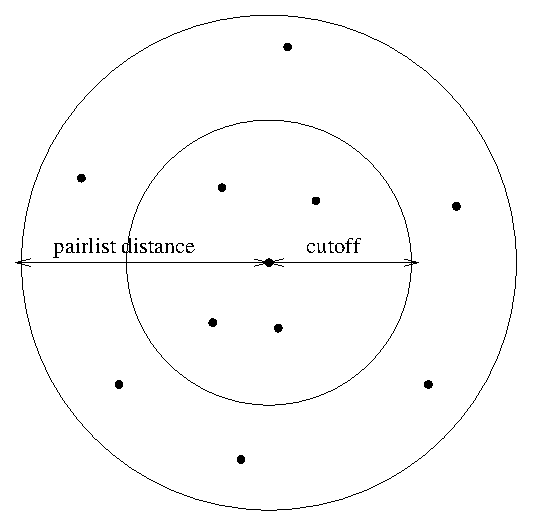
\includegraphics{figures/pairlistdist}}
  \caption[Example of cutoff and pairlist distance uses]
  {{\small Depiction of the difference between the cutoff distance and the
  pair list distance.  The pair list distance specifies a sphere that is
  slightly larger than that of the cutoff so that pairs are allowed to
  move in and out of the cutoff distance without causing energy conservation
  to be disturbed.}}
  \label{fig:pairlistdist}
\end{figure}

The {\tt pairlistdist} parameter is also used to determine the minimum patch size.
Unless the {\tt splitPatch} parameter is explicitly set to {\tt position}, hydrogen atoms will be placed on the same patch as the ``mother atom'' to which they are bonded.
These {\em hydrogen groups} are then distance tested against each other using only a cutoff increased by the the value of the {\tt hgroupCutoff} parameter.
The size of the patches is also increased by this amount.
\NAMD\ functions correctly even if a hydrogen atom and its mother atom are separated by more than half of {\tt hgroupCutoff} by breaking that group into its individual atoms for distance testing.
Margin violation warning messages are printed if an atom moves outside of a safe zone surrounding the patch to which it is assigned, indicating that {\tt pairlistdist} should be increased in order for forces to be calculated correctly and energy to be conserved.

\index{margin violations}
Margin violations mean that atoms that are in non-neighboring patches may
be closer than the cutoff distance apart.  This may sometimes happen in
constant pressure simulations when the cell shrinks (since the patch grid
remains the same size).  The workaround is to increase the margin
parameter so that the simulation starts with fewer, larger patches.
Restarting the simulation will also regenerate the patch grid.

In rare special circumstances atoms that are involved in bonded terms
(bonds, angles, dihedrals, or impropers) or nonbonded exclusions (especially
implicit exclusions due to bonds) will be placed on non-neighboring
patches because they are more than the cutoff distance apart.  This can
result in the simulation dying with a message of
``bad global exclusion count''.
\index{Atoms moving too fast}
\index{error message!Atoms moving too fast}
\index{Bad global exclusion count}
\index{error message!Bad global exclusion count}
If an ``atoms moving too fast; simulation has become unstable'',
``bad global exclusion count'', or similar error happens
on the first timestep then there is likely something very
wrong with the input coordinates, such as the atoms with uninitialized
coordinates or different atom orders in the PSF and PDB file.  Looking at
the system in VMD will often reveal an abnormal structure.
Be aware that the atom IDs in the ``Atoms moving too fast'' error
message are 1-based, while VMD's atom indices are 0-based.
If an ``atoms moving too fast; simulation has become unstable'',
``bad global exclusion count'', or similar error happens
later in the simulation then the dynamics have
probably become unstable, resulting in the system ``exploding'' apart.
Energies printed at every timestep should show an exponential increase.
This may be due to a timestep that is too long, or some other strange
feature.  Saving a trajectory of every step and working backwards in
can also sometimes reveal the origin of the instability.


\begin{itemize}

\item
\NAMDCONFWDEF{pairlistdist}
{distance between pairs for inclusion in pair lists (\AA)}
{positive decimal $\geq$ {\tt cutoff}}
{{\tt cutoff}}
{
A pair list is generated {\tt pairlistsPerCycle} times each cycle, 
containing pairs of atoms for which 
electrostatics and van der Waals interactions will be calculated.
This parameter is used when {\tt switching} is set to {\tt on} to
specify the allowable distance between atoms for inclusion in the
pair list.  
This parameter is equivalent to the X-PLOR parameter {\tt CUTNb}.
If no atom moves more than {\tt pairlistdist}$-${\tt cutoff} during
one cycle, then there will be no jump in electrostatic or van der
Waals energies when the next pair list is built.  Since such a jump
is unavoidable when truncation is used, this parameter may only
be specified when {\tt switching} is set to {\tt on}.  If this
parameter is not specified and {\tt switching} is set to {\tt on},
the value of {\tt cutoff} is used.  
A value of at least one greater than {\tt cutoff} is recommended.  
}

\item
\NAMDCONFWDEF{stepspercycle}{timesteps per cycle}{positive integer}{20}
{Number of timesteps in each cycle.  Each cycle represents the number 
of timesteps between atom reassignments.
For more details on non-bonded force evaluation, see
Section \ref{section:electdesc}.}

\item
\NAMDCONFWDEF{splitPatch}
{how to assign atoms to patches}
{{\tt position} or {\tt hydrogen}}
{{\tt hydrogen}}
{
When set to {\tt hydrogen}, hydrogen atoms are kept on the same patch as their parents, allowing faster distance checking and rigid bonds.
}

\item
\NAMDCONFWDEF{hgroupCutoff (\AA)}
{used for group-based distance testing}
{positive decimal}
{2.5}
{
This should be set to twice the largest distance which will ever occur between a hydrogen atom and its mother.  Warnings will be printed if this is not the case.  This value is also added to the margin.
}

\item
\NAMDCONFWDEF{margin}
{extra length in patch dimension (\AA)}{positive decimal}{0.0}
{An internal tuning parameter used in determining the size of the cubes 
of space with which \NAMD\ uses to partition the system.  The value of 
this parameter will not change the physical results of the simulation.  
Unless you are very motivated to get the {\it very} best 
possible performance, just leave this value at the default.}

\item
\NAMDCONFWDEF{pairlistMinProcs}{min procs for pairlists}
{positive integer}{1}
{
Pairlists may consume a large amount of memory as atom counts, densities,
and cutoff distances increase.  Since this data is distributed across
processors it is normally only problematic for small processor counts.
Set pairlistMinProcs to the smallest number of processors on which
the simulation can fit into memory when pairlists are used.
}

\item
\NAMDCONFWDEF{pairlistsPerCycle}{regenerate x times per cycle}
{positive integer}{2}
{
Rather than only regenerating the pairlist at the beginning of a cycle,
regenerate multiple times in order to better balance the costs of
atom migration, pairlist generation, and larger pairlists.
}

\item
\NAMDCONFWDEF{outputPairlists}{how often to print warnings}
{non-negative integer}{0}
{
If an atom moves further than the pairlist tolerance during a simulation
(initially (pairlistdist - cutoff)/2 but refined during the run) any
pairlists covering that atom are invalidated and temporary pairlists
are used until the next full pairlist regeneration.  All interactions
are calculated correctly, but efficiency may be degraded.  Enabling
outputPairlists will summarize these pairlist violation warnings
periodically during the run.
}

\item
\NAMDCONFWDEF{pairlistShrink}{tol *= (1 - x) on regeneration}
{non-negative decimal}{0.01}
{
In order to maintain validity for the pairlist for an entire cycle,
the pairlist tolerance (the distance an atom can move without causing
the pairlist to be invalidated) is adjusted during the simulation.
Every time pairlists are regenerated the tolerance is reduced by
this fraction.
}

\item
\NAMDCONFWDEF{pairlistGrow}{tol *= (1 + x) on trigger}
{non-negative decimal}{0.01}
{
In order to maintain validity for the pairlist for an entire cycle,
the pairlist tolerance (the distance an atom can move without causing
the pairlist to be invalidated) is adjusted during the simulation.
Every time an atom exceeds a trigger criterion that is some fraction
of the tolerance distance, the tolerance is increased by this fraction.
}

\item
\NAMDCONFWDEF{pairlistTrigger}{trigger is atom beyond (1 - x) * tol}
{non-negative decimal}{0.3}
{
The goal of pairlist tolerance adjustment is to make pairlist invalidations
rare while keeping the tolerance as small as possible for best performance.
Rather than monitoring the (very rare) case where atoms actually move more
than the tolerance distance, we reduce the trigger tolerance by this
fraction.  The tolerance is increased whenever the trigger tolerance is
exceeded, as specified by pairlistGrow.
}

\end{itemize}


% User defined forces
\newpage

\section{User Defined Forces}
\label{section:userdef}


%\subsection{Applied Forces and Analysis}

There are several ways to apply external forces to simulations with \NAMD.
These are described below.


\subsection{Constant Forces}

NAMD provides the ability to apply constant forces to some atoms.
There are two parameters that control this feature.

\begin{itemize}

\item
\NAMDCONFWDEF{constantForce}{Apply constant forces?}{yes or no}{no}
{Specifies whether or not constant forces are applied.}

\item
\NAMDCONF{consForceFile}{PDB file containing forces to be applied}{UNIX filename}
{
The X, Y, Z and occupancy (O) fields of this file are read to
determine the constant force vector of each atom, which is
(X,Y,Z)*O, in unit of kcal/(mol*\AA). The occupancy (O) serves as
a scaling factor, which could expand the range of the force
applied. (One may be unable to record very large or very small
numbers in the data fields of a PDB file due to limited space).
Zero forces are ignored.

Specifying {\tt consforcefile} is optional; constant forces may be specified
or updated between runs by using the \icommand{consForceConfig} command.
}

\item
\NAMDCONFWDEF{consForceScaling}{Scaling factor for constant forces}{decimal}{1.0}
{Scaling factor by which constant forces are multiplied.  May be changed between run commands.}

\end{itemize}


\subsection{External Electric Field}

\NAMD\ provides the ability to apply a constant electric field to the molecular
system being simulated.
Energy due to the external field will be reported in the MISC column
and may be discontinuous in simulations using periodic boundary conditions if,
for example, a charged hydrogen group moves outside of the central cell.
There are two parameters that control this feature.

\begin{itemize}

\item
\NAMDCONFWDEF{eFieldOn}{apply electric field?}{{\tt yes} or {\tt no}}{{\tt no}}
{Specifies whether or not an electric field is applied.}

\item
\NAMDCONF{eField}{electric field vector}{vector of decimals (x y z)}
{Vector which describes the electric field to be applied.
Units are ${\rm kcal} / ({\rm mol \; \AA} \; e)$, which is natural for simulations.
This parameter may be changed between {\tt run} commands, allowing a square
wave or other approximate wave form to be applied.}

\end{itemize}

\subsection{Grid Forces}

\NAMD\ provides the ability to specify grids describing a potential in the simulation 
space. Each atom is affected by the potential based on its charge and its position, 
using the potential function interpolated from the specified grid(s). Energy due to the 
grid-defined field will be reported in the MISC column of the output, unless a scaling
factor not proportional to (1,1,1) is used.

NAMD allows the definition of multiple grids, each with a separate set of defining 
parameters. This is specified using a tag field in each of the mgridforceXXX commands. 
The tag is an alphanumeric string without spaces which identifies to which grid the 
specified field applies.

The grid file format is a subset of the DataExplorer DX file format, as shown below:
\begin{verbatim}
# Lines at the beginning of the file starting with a # symbol 
# are ignored as comments
# Variables (replaced by numbers in an actual file):
#   xn, yn, and zn are the number of data points along each dimension;
#   xorg, yorg, and zorg is the origin of the grid, in angstroms;
#   x[1-3]del, y[1-3]del, and z[1-3]del are the basis vectors which transform
#   grid indices to coordinates in angstroms:
#      x(i,j,k) = xorg + i * x1del + j * y1del + k * z1del
#      y(i,j,k) = yorg + i * x2del + j * y2del + k * z2del
#      z(i,j,k) = zorg + i * x3del + j * y3del + k * z3del
#
#   Grid data follows, with three values per line, ordered z fast, y medium,
#   and x slow. Exactly xn*yn*zn values should be given. Grid data is then
#   terminated with a field object.
#   
#  Note: Other features of the DX file format are not handled by this code
#
object 1 class gridpositions counts xn yn zn
origin xorg yorg zorg
delta x1del y1del z1del
delta x2del y2del z2del
delta x3del y3del z3del
object 2 class gridconnections counts xn yn zn
object 3 class array type double rank 0 items [ xn*yn*zn ] data follows
f1 f2 f3
f4 f5 f6
.
.
.
object 4 class field
component "positions" value 1
component "connections" value 2
component "data" value 3
\end{verbatim}

Each dimension of the grid may be specified as continuous or not. If the grid is not continuous in a particular dimension, the potential grid is padded with one border slices on each non-continuous face of the grid, and border grid values are computed so that the force felt by an atom outside the grid goes to zero. If the grid is continuous along a particular dimension, atoms outside the grid are affected by a potential that is interpolated from the grid and its corresponding periodic image along that dimension.

To calculate the force on an atom due to the grid, the atom's coordinates are transformed according to the current basis vectors of the simulation box to a coordinate frame that is centered at the center of the specified grid. Note that the size and spatial coordinates of the grid remain fixed, and are not scaled as the size of the simulation box fluctuates. For atoms within the grid, the force is computed by analytically determining the gradient of the tricubic polynomial used to interpolate the potential from surrounding grid values. For atoms outside the grid, the state of the {\tt mgridforcecont[1,2,3]} determine whether the force is zero, or computed from the images of the grid as described above. Note that if the grid is ever larger than the periodic box, it is truncated at the edge of that box. The consequence of this is that the computed potential will not vary smoothly at the edges, introducing numerical instability.

NAMD also supports non-uniform grids, allowing regions of a grid to be defined at higher resolution.
Non-uniform grids are structured hierarchically, with a single \emph{maingrid} which has one or more \emph{subgrid}s.
Each subgrid spans a number of maingrid cells in each of the three dimensions, and effectively redefines the data in that region.
The subgrids are usually defined at higher resolution, with the restriction that the number of cells along each dimension is an integral number of the original number in the maingrid.
Note that the maingrid still has data points in regions where subgrids are defined, and that, on the boundary of a subgrid, \emph{they must agree with the values in the subgrid}.
Subgrids, in turn, may have subgrids of their own, which may have subgrids of their own, etc.

A non-uniform grid file takes the form of a special comment block followed by multiple normal grid definitions.
The special comment block defines the grid hierarchy, and consists of comments beginning with {\tt \# namdnugrid}.
An example follows:
\begin{verbatim}
# namdnugrid version 1.0
# namdnugrid maingrid subgrids count 2
# namdnugrid subgrid 1 generation 1 min x1 y1 z1 max x2 y2 z2 subgrids count 2
# namdnugrid subgrid 2 generation 2 min x3 y3 z3 max x4 y4 z4 subgrids count 0
# namdnugrid subgrid 3 generation 2 min x5 y5 z5 max x6 y6 z6 subgrids count 0
# namdnugrid subgrid 4 generation 1 min x7 y7 z7 max x8 y8 z8 subgrids count 0
\end{verbatim}
The maingrid is described by the number of subgrids.
Subgrids are additionally described by a subgrid number; a generation number, which should be one higher than the generation of its supergrid; and {\tt min} and {\tt max} attributes, which describe the location of the subgrid within its supergrid.
In this example, the maingrid has two subgrids, subgrid 1 and subgrid 4, labeled {\tt generation 1}.
The first of these subgrids has two subgrids of its own ({\tt generation 2}).
Notice that subgrids are described immediately after their supergrid.
The {\tt min} and {\tt max} attributes are given in units of grid \emph{cells} of the supergrid.
For example, a subgrid with {\tt min 0 0 0 max 1 1 1} would redefine 8 cells of its supergrid, the space between gridpoints (0, 0, 0) and (2, 2, 2) in grid coordinates.
Following the comment block, the maingrid and subgrids are defined in the format described above, in the same order as the comment block.


The following parameters describe the grid-based potentials.

\begin{itemize}

\item
\NAMDCONFWDEF{mgridforce}
{apply grid forces?}
{{\tt yes} or {\tt no}}{{\tt no}}
{Specifies whether or not any grid forces are being applied.}

\item
\NAMDCONFTAG{mgridforcefile}
{PDB file specifying force multipliers and charges for each atomd}
{UNIX file name}
{The force on each atom is scaled by the corresponding value in this PDB file. By setting the force multiplier to zero for an atom, it will not be affected by the grid force. }

\item
\NAMDCONFTAGWDEF{mgridforcecol}
{column of PDB from which to read force multipliers}
{X, Y, Z, O, or B}
{B}
{Which column in the PDB file specified by {\tt mgridforcefile} contains the scaling factor}

\item
\NAMDCONFTAGWDEF{mgridforcechargecol}
{column of PDB from which to read atom charges}
{X, Y, Z, O, or B}
{Atom charge used for electrostatics.} 
{Which column in the PDB file specified by {\tt mgridforcefile} contains the atom charge. By default, the charge value specified for the short-range Columb interactions are also used for the grid force. Both {\tt mgridforcecol} and {\tt mgridforceqcol} can be specified, in which case the apparent charge of the atom will be the product of the two values.}

\item
\NAMDCONFTAG{mgridforcepotfile}
{grid potential file name}
{UNIX file name}
{File specifying the grid size, coordinates, and potential values.}

\item
\NAMDCONFTAGWDEF{mgridforcevolts}
{grid potential units in eV/charge}
{{\tt yes} or {\tt no}}{{\tt no}}
{If set, the grid potential values are expressed in {\rm eV}. Otherwise, values are
in ${\rm kcal} / ({\rm mol} \; charge)$}

\item
\NAMDCONFTAGWDEF{mgridforcescale}
{scale factor for grid potential}
{Vector of decimals {\it scale}$_x$ {\it scale}$_y$ {\it scale}$_z$ }
{1 1 1}
{Scale factor applied to the grid potential values}

\item
\NAMDCONFTAGWDEF{mgridforcecont1}
{Is grid continuous in the direction of the first basis vector}
{{\tt yes} or {\tt no}}{{\tt no}}
{By specifying that the grid is continuous in a direction, atoms outside of the grid will be affected by a force determined by interpolating based on the values at the edge of the grid with the values of the corresponding edge of the periodic image of the grid. The current size of the simulation box is taken into account, so that as the simulation box size fluctuates, the force on an atom outside of the grid varies continuously until it re-enters the opposite edge of the grid. If the grid is not continuous in this direction, the interpolated force on atoms near the edge of the grid is calculated so that it continuously approaches zero as an atom approaches the edge of the grid.}

\item
\NAMDCONFTAGWDEF{mgridforcecont2}
{Is grid continuous in the direction of the second basis vector}
{{\tt yes} or {\tt no}}{{\tt no}}
{Operates the same as {\tt mgridforcecont1} except applies in the direction of the second basis vector}

\item
\NAMDCONFTAGWDEF{mgridforcecont3}
{Is grid continuous in the direction of the third basis vector}
{{\tt yes} or {\tt no}}{{\tt no}}
{Operates the same as {\tt mgridforcecont1} except applies in the direction of the third basis vector}

\item
\NAMDCONFTAGWDEF{mgridforcevoff}
{Offset periodic images of the grid by specified amounts}
{vector of decimals (x y z)}
{(0 0 0)}
{If a continuous grid is used along a particular basis vector, it may be desirable to shift the potentials in the image to manipulate the potential outside the grid. For example, consider the case where the potential is a ramp in the $x$ direction and the grid is defined for points $[0,N)$, with a potential $f(i,j,k)$ given by $f(i,j,k) = f_0 + i (f_1-f_0) / N$. By shifting the images of the grid, the potential can be transformed as illustrated in Fig.~\ref{fig:gridshift}.
}

\begin{figure}[htb]
  \center{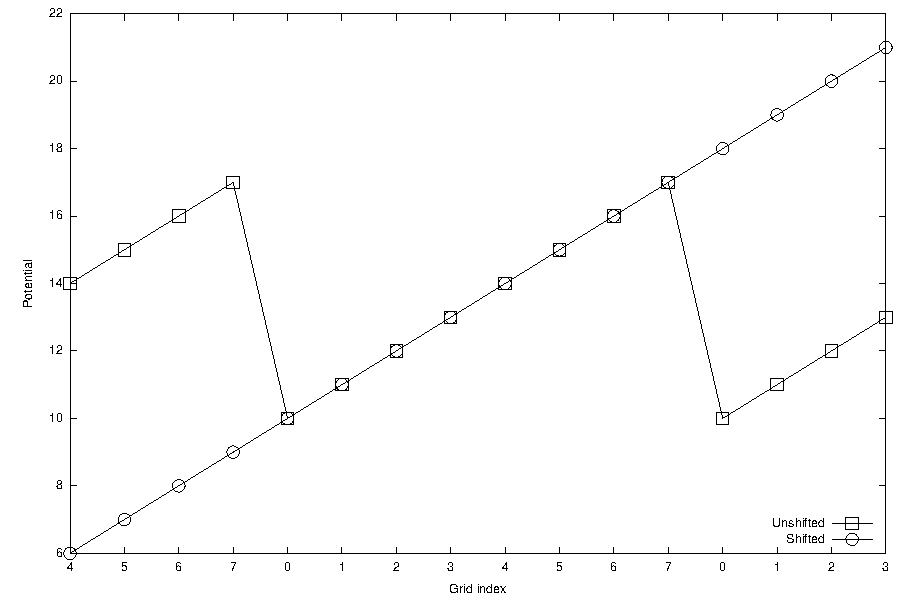
\includegraphics{figures/gridshift}}
  \caption[Graph showing a slice of a ramp potential, showing the effect of 
           {\tt mgridforcevoff}]
  {\small Graph showing a slice of a ramp potential, with eight grid points along the axis, and a periodic cell size which just contains the grid. The Unshifted case shows how the pontential is not smooth when {\tt mgridforcevoff} is not specified, or set to zero. The Shifted potential shows the grid that results when {\tt mgridfocevoff} is set so that the wrapped potential is offset so that the potential has constant slope at the periodic boundaries.}
  \label{fig:gridshift}
\end{figure}

\item
\NAMDCONFTAGWDEF{mgridforcelite}
{Is grid to use Gridforce Lite interpolation?}
{{\tt yes} or {\tt no}}
{{\tt no}}
{When Gridforce Lite is enabled, a faster but less accurate interpolation method is used to compute forces.
Specifically, rather than computing a tri-cubic interpolation of the potential, from which the force is then computed analytically, Gridforce Lite computes force as a linear interpolation.
This method also increases the memory required by Gridforce.
Note that Gridforce Lite is incompatible with use of the {\tt mgridforcecont[123]} keywords and with non-uniform grids.
}

\end{itemize}

\subsection{Moving Constraints}

Moving constraints feature works in conjunction with the Harmonic
Constraints (see an appropriate section of the User's guide).
The reference positions of all constraints
will move according to
\begin{equation}
\label{eq:smdrefpos}
   \vec r(t) \; = \; \vec r_0 \, + \, \vec v t \,.
\end{equation}
A velocity vector $\vec v$ ({\tt movingConsVel}) needs to be specified.

The way the moving constraints work is that the moving reference
position is calculated every integration time step using
Eq.~\ref{eq:smdrefpos}, where $\vec v$ is in \AA/timestep, and $t$ is the
current timestep (i.e., {\tt firstTimestep} plus however many
timesteps have passed since the beginning of \NAMD\ run). Therefore,
one should be careful when restarting simulations to appropriately
update the {\tt firstTimestep} parameter in the \NAMD\ configuration
file or the reference position specified in the reference PDB file.

\noindent {\bf NOTE: } \NAMD\ actually calculates the constraints
potential with $U = k (x-x_0)^d$ and the force with $F = d k (x-x_0)$,
where $d$ is the exponent {\tt consexp}. The result is that if one
specifies some value for the force constant $k$ in the PDB file,
effectively, the force constant is $2 k$ in calculations. This caveat
was removed in SMD feature.

The following parameters describe the parameters for the
moving harmonic constraint feature of \NAMD.

\begin{itemize}

\item
\NAMDCONFWDEF{movingConstraints}{Are moving constraints active}
{{\tt on} or {\tt off}}{{\tt off}}
{Should moving restraints be applied to the system. If set
to {\tt on}, then  {\tt movingConsVel} must be defined.
May not be used with {\tt rotConstraints}.}

\item
\NAMDCONF{movingConsVel}{Velocity of the reference position movement}
{vector in \AA/timestep}
{The velocity of the reference position movement. Gives both absolute
value and direction}

\end{itemize}

\subsection{Rotating Constraints}

The constraints parameters are specified in the same manner as for
usual (static) harmonic constraints. The reference positions of all
constrained atoms are then rotated with a given angular velocity
about a given axis. If the force constant of the constraints is
sufficiently
large, the constrained atoms will follow their reference positions.

A rotation matrix $M$ about the axis unit vector $v$ is calculated every
timestep
for the angle of rotation corresponding to the current timestep.
    angle = $\Omega t$,
where $\Omega$ is the angular velocity of rotation.

From now on, all quantities are 3D vectors, except the matrix $M$ and the
force constant $K$.

The current reference position $R$ is calculated from the initial
reference
position $R_0$ (at $t=0$),
    $R = M (R_0 - P) + P$,
where $P$ is the pivot point.

%geometry of rotation:
%
%
%
%                        * R
%                      / |
%                    /   |
%                  /     | normal to axis
%                /       |
%            P /         |
%        ----*--->-------*---------------------> axis
%                v       N

Coordinates of point N can be found as
   $N = P + ( (R - P) \cdot v ) v$.
Normal from the atom pos to the axis is, similarly,
   normal $= ( P + ( (X - P) \cdot v ) v ) - X$
The force is, as usual,
   $F = K (R - X)$;
This is the force applied to the atom in NAMD (see below).
NAMD does not know anything about the torque
applied. However, the torque applied to the atom can be calculated
as a vector product
   torque $= F \times normal$
Finally, the torque applied to the atom with respect to the axis
is the projection of the torque on the axis, i.e.,
   $torque_{proj} = torque \cdot v$

If there are atoms that have to be constrained, but not moved,
this implementation is not suitable, because it will move {\em all}
reference positions.

Only one of the moving and rotating constraints can be used at a
time.

Using very soft springs for rotating constraints leads to the system
   lagging behind the reference positions, and then the force is applied
   along a direction different from the "ideal" direction along the
   circular path.

Pulling on N atoms at the same time with a spring of stiffness K
   amounts to pulling on the whole system by a spring of stiffness NK,
   so the overall behavior of the system is as if you are pulling with a
   very stiff spring if N is large.

In both moving and rotating constraints the force constant that you
   specify in the constraints pdb file is multiplied by 2 for the force
   calculation, i.e., if you specified $K = 0.5 \; {\rm kcal}/{\rm mol}/{\rm \AA}^2$ in the pdb
file,
   the force actually calculated is $F = 2 K (R-X) = 1 \; {\rm kcal}/{\rm mol}/{\rm \AA}^2 \; (R-X)$.
   SMD feature of namd2 does the calculation without multiplication of
the
   force constant specified in the config file by 2.


\begin{itemize}

\item
\NAMDCONFWDEF{rotConstraints}{Are rotating constraints active}
{{\tt on} or {\tt off}}{{\tt off}}
{Should rotating restraints be applied to the system. If set
to {\tt on}, then {\tt rotConsAxis}, {\tt rotConsPivot} and
{\tt rotConsVel} must be defined.
May not be used with {\tt movingConstraints}.}

\item
\NAMDCONF{rotConsAxis}{Axis of rotation}
{vector (may be unnormalized)}
{Axis of rotation. Can be any vector. It gets
normalized before use. If the vector is 0,
no rotation will be performed, but the calculations
will still be done.}

\item
\NAMDCONF{rotConsPivot}{Pivot point of rotation}
{position in \AA}
{Pivot point of rotation. The rotation axis vector
only gives the direction of the axis. Pivot point
places the axis in space, so that the axis goes
through the pivot point.}

\item
\NAMDCONF{rotConsVel}{Angular velocity of rotation}
{rate in degrees per timestep}
{Angular velocity of rotation, degrees/timestep.}

\end{itemize}

\subsection{Symmetry Restraints}
Symmetry restraints are based on symmetrical relationships
between monomers.  Defined monomers are transformed to overlap
and an average position for each atom is calculated.  After the average 
structure is transformed back, a harmonic force is calculated which 
drives each monomer to the average.

\begin{itemize}
\item
\NAMDCONFWDEF{symmetryRestraints}{Are symmetry restraints active?}{{\tt on} or {\tt off}}{{\tt off}}
{Should Symmetry constraining forces be applied to the system.  If symmetry restraints are enabled,
{\tt symmetryk}* and {\tt symmetryFile} must be defined in the 
input file as well.  *See {\tt symmetryk} entry for details.}

\item
\NAMDCONFWDEF{symmetryFirstFullStep}{First step to apply full harmonic force}{Non-negative integer}{{\tt symmetryFirstStep}}
{Force constant {\tt symmetryk} linearly increased from {\tt symmetryFirstStep} to {\tt symmetryFirstFullStep}}

\item
\NAMDCONFWDEF{symmetryLastFullStep}{Last step to apply full harmonic force}{Non-negative integer}{{\tt symmetryLastStep}}
{Force constant {\tt symmetryk} linearly decreased from {\tt symmetryLastFullStep} to {\tt symmetryLastStep}} 

\item
\NAMDCONF{symmetryk}{Constant for harmonic restraining forces}
{Positive value}
{Harmonic force constant.  Scaled down by number of atoms in the monomer.  If this setting is omitted, the value in the occupancy column
of the pdb file specified by {\tt symmetrykFile} will be used as the constant for that atom.  
This allows the user to specify the constant on a per-atom basis.}

\item
\NAMDCONF{symmetrykFile}{pdb containing per atom force constants}{Path to pdb file}
{pdb where the occupancy column specifies the per atom force constants.  If using overlapping
symmetry groups, you must include one additional {\tt symmetrykfile} per {\tt symmetryFile} }

\item
\NAMDCONFWDEF{symmetryScaleForces}{Scale symmetry restraints over time}{{\tt on} or {\tt off}}{{\tt off}}
{If turned on, the harmonic force applied by the symmetry restraints will linearly evolve with each time step based on
{\tt symmetryFirstFullStep} and {\tt symmetryLastFullStep}.}

\item
\NAMDCONF{symmetryFile}{File for symmetry information}
{Path to PDB file}
{
Restrained atoms are those whose occupancy (O) is nonzero in the symmetry pdb file.
The file must contain no more atoms than the structure file and those atoms
present must have the exact same index as the structure file (i.e., the file
may contain a truncated atom selection ``index $< N$'' but not an arbitrary selection).
The value in
the occupancy column represent the "symmetry group" the atom belongs to.  These symmetry
groups are used for denoting monomers of the same type.  These groups will be transformed by the
matrices in their own {\tt symmetryMatrixFile} and averaged separetely from other groups.  
The designation in the occupancy column should be an integer value starting at 1 and proceeding
in ascending order, mirroring the order of the corresponding matrix file within the configuration file
(e.g. the first symmetryMatrixFile contains the matrices for symmetry group 1).  
The value in the atom's beta column represents its monomer designation.  This should be an integer
value starting at 1 and proceeding in ascending order, relative to the order of the corresponding
transformation matrix found in the symmetry group's {\tt symmetryMatrixFile}.
If an atom is contained in more than one symmetry group, additional pdb files can be listed.
These pdb files should follow the same rules as the first one (unique group and monomer identifiers
in increasing order).  
}

\item
\NAMDCONF{symmetryMatrixFile}{File for transformation matrices}
{Path to matrix file}
{
The {\tt symmetryMatrixFile} is a path to a file that contains a list of transformation
matrices to make the monomers overlap.  The file should contain one (and only one)
matrix for each monomer in the order of monomer ID designated in the symmetryFile.
Each symmetry group should have its own symmetryMatrixFile file containing only the matrices
used by the monomers in that group.  
These should be formatted with spaces between columns and
NO spaces between rows as follows:

1 0 0 0 \\
0 1 0 0 \\
0 0 1 0 \\ 
0 0 0 1 \\

with different matrices separated by a single blank line (and no line before the first or after
the last matrix).  This file is
OPTIONAL.  Leave this line out to have namd generate the transformations
for you.
}
\item
\NAMDCONFWDEF{symmetryFirstStep}{first symmetry restraint timestep}{Non-negative integer}{0} {}
\item
\NAMDCONFWDEF{symmetryLastStep}{last symmetry restraint timestep}{Positive integer}{infinity}
{ Symmetry restraints are applied only between {\tt symmetryFirstStep} and {\tt symmetryLastStep}.
Use these settings with caution and ensure restraints are only being applied when necessary (e.g. not
during equilibration).  }

\end{itemize}

\subsection{Targeted Molecular Dynamics (TMD)}

In TMD, subset of atoms in the simulation is guided towards a 
final 'target' structure by means of steering forces.  At each timestep, 
the RMS distance between
the current coordinates and the target structure is computed (after
first aligning the target structure to the current coordinates).
The force on each atom is given by the gradient of the potential
\begin{equation}
U_{TMD} = \frac{1}{2} \frac{k}{N} \left[ RMS(t) - RMS^*(t) \right]^2
\label{eq:tmdpotential}
\end{equation}
where $RMS(t)$ is the instantaneous best-fit RMS distance of the current
coordinates from the target coordinates, and $RMS^*(t)$ evolves linearly
from the initial RMSD at the first TMD step to the final RMSD at the last 
TMD step.  The spring constant $k$ is scaled down by the number $N$ of targeted
atoms.

Atoms can be separated into non-overlapping constraint domains by
assigning integer values in the beta column of the {\tt TMDFile}.  Forces on
the atoms will be calculated for each domain independently of the other domains.

Within each domain, the set of atoms used to fit the target structure can be
different from the set of atoms that are biased towards the target structure.
If the altloc field in the {\tt TMDFile} is not ` ' or `0' then the atom is fitted.
If the occupancy is non-zero then the atom is biased.
If none of the atoms in a domain have altloc set then all biased atoms are fitted.

Note that using different atoms for fitting and biasing
or not using the same spring constant for all target atoms within
a domain will result in forces conserving neither energy nor momentum.
In this case harmonic restraints and Langevin dynamics are likely needed.

\begin{itemize}
\item
\NAMDCONFWDEF{TMD}{Is TMD active}{{\tt on} or {\tt off}}{{\tt off}}
{Should TMD steering forces be applied to the system.  If TMD is enabled,
{\tt TMDk}, {\tt TMDFile}, and {\tt TMDLastStep} must be defined in the 
input file as well.}

\item
\NAMDCONF{TMDk}{Elastic constant for TMD forces}
{Positive value in $kcal/mol/$\AA$^2$.}
{The value of $k$ in Eq.~\ref{eq:tmdpotential}.  A value of 200 seems to work
well in many cases.  If this setting is omitted, the value in the occupancy column
of the pdb file specified by {\tt TMDFile} will be used as the constant for that atom.  
This allows the user to specify the constant on a per-atom basis.}

\item
\NAMDCONFWDEF{TMDOutputFreq}{How often to print TMD output}{Positive integer}
{1} 
{ TMD output consists of lines of the form {\tt TMD  ts  targetRMS  currentRMS}
where {\tt ts} is the timestep, {\tt targetRMS} is the target RMSD at that 
timestep, and {\tt currentRMS} is the actual RMSD.}

\item
\NAMDCONF{TMDFile}{File for TMD information}
{Path to PDB file}
{
Biased atoms are those whose occupancy (O) is nonzero in the TMD PDB file.
Fitted atoms are those whose altloc field is not ` ' or `0', if present,
otherwise all biased atoms are fitted.
The file must contain no more atoms than the structure file and those atoms
present must have the exact same index as the structure file (i.e., the file
may contain a truncated atom selection ``index $< N$'' but not an arbitrary selection).
The coordinates for the target structure are also taken from the targeted
atoms in this file.  Non-targeted atoms are ignored.  The beta column of targetted
atoms is used to designate non-overlapping constraint domains.  Forces will be
calculated for atoms within a domain separately from atoms of other domains.
}

\item
\NAMDCONFWDEF{TMDFirstStep}{first TMD timestep}{Positive integer}{0} {}
\item
\NAMDCONF{TMDLastStep}{last TMD timestep}{Positive integer}
{ TMD forces are applied only between {\tt TMDFirstStep} and {\tt TMDLastStep}.
The target RMSD evolves linearly in time from the initial to the final target 
value.  }

\item
\NAMDCONFWDEF{TMDInitialRMSD}{target RMSD at first TMD step}
{Non-negative value in \AA}{from coordinates}{
In order to perform TMD calculations that involve restarting a previous
NAMD run, be sure to specify {\tt TMDInitialRMSD} with the same value
in each NAMD input file, and use the NAMD parameter {\tt firstTimestep}
in the continuation runs so that the target RMSD continues from where the
last run left off.
}
\item
\NAMDCONFWDEF{TMDFinalRMSD}{target RMSD at last TMD step}
{Non-negative value in \AA}{0}
{If no {\tt TMDInitialRMSD} is given, the initial RMSD will be calculated at the
first TMD step.  {\tt TMDFinalRMSD} may be less than or greater than
{\tt TMDInitialRMSD}, depending on whether the system is to be steered 
towards or away from a target structure, respectively.  Forces are applied
only if $RMS(t)$ is betwween {\tt TMDInitialRMSD} and $RMS*(t)$; in other
words, only if the current RMSD fails to keep pace with the target value.}

\item
\NAMDCONFWDEF{TMDDiffRMSD}{Is double-sided TMD active?}{{\tt on} or {\tt off}}{{\tt off}}
{Turns on the double-sided TMD feature which targets the transition between two structures. 
This is accomplished by modifying the TMD force such that the potential is based on the
difference of RMSD's from the two structures:
\begin{equation}
U_{TMD} = \frac{1}{2} \frac{k}{N} \left[ DRMS(t) - DRMS^*(t) \right]^2
\label{eq:dstmdpotential}
\end{equation}
where $DRMS(t)$ is RMS1(t) - RMS2(2) (RMS1 being the RMSD from structure 1 and RMS2 the RMSD from structure 2).
The first structure is specified as normal in {\tt TMDFile} and the second structure should
be specified in {\tt TMDFile2}, preserving any domain designations found in {\tt TMDFile}. 
}

\item
\NAMDCONF{TMDFile2}{Second structure file for double-sided TMD}
{Path to PDB file}
{PDB file defining the second structure of a double sided TMD. This file
should contain the same number of atoms as {\tt TMDFile} along with the 
same domain designations if any are specified.
}

\end{itemize}

\subsection{Steered Molecular Dynamics (SMD)}

The SMD feature is independent from the harmonic constraints, although it
follows the same ideas.  In both SMD and harmonic constraints, one specifies
a PDB file which indicates which atoms are 'tagged' as constrained.  The PDB
file also gives initial coordinates for the constraint positions.  One also
specifies such parameters as the force constant(s) for the constraints, 
and the velocity with which the constraints move.  

There are two major differences between SMD and
harmonic constraints:
\begin{itemize}
\item In harmonic constraints, each tagged atom is harmonically constrained
  to a reference point which moves with constant velocity.  In SMD, it is
  the {\em center of mass} of the tagged atoms which is constrained to move
  with constant velocity.

\item In harmonic constraints, each tagged atom is constrained in all three
  spatial dimensions.  In SMD, tagged atoms are constrained {\em only along
  the constraint direction} (unless the optional {\tt SMDk2} keyword is used.)
\end{itemize}

The center of mass of the SMD atoms will be harmonically constrained with 
force constant $k$ ({\tt SMDk}) to move with velocity $v$ ({\tt SMDVel}) in 
the direction $\vec n$ ({\tt SMDDir}).  SMD thus results in the following
potential being applied to the system:
\begin{equation}
\label{eq:SMDpotential}
U(\vec r_1, \vec r_2, ..., t) \; = \; \frac{1}{2} 
  k\left[vt - (\vec R(t) - \vec R_0)\cdot \vec n \right]^2.
\end{equation}
Here, $t \equiv N_{ts} dt$ where $N_{ts}$ is the number of elapsed timesteps
in the simulation and $dt$ is the size of the timestep in femtoseconds.
Also, $\vec R(t)$ is the current center of mass of the SMD atoms and $R_0$ is
the initial center of mass as defined by the coordinates in {\tt SMDFile}.
Vector $\vec n$ is normalized by \NAMD\ before being used.

Optionally, one may also specify a transverse force constant $k_2$ ({\tt SMDk2}).
The potential then becomes
\begin{equation}
\label{eq:SMDpotential2}
U(\vec r_1, \vec r_2, ..., t) \; = \; \frac{1}{2} 
  k\left[vt - (\vec R(t) - \vec R_0)\cdot \vec n \right]^2 + \frac{1}{2}k_2\left[\left(\vec R(t) - \vec R_0\right)^2 - \left((\vec R(t) - \vec R_0) \cdot \vec n\right)^2\right].
\end{equation}
In this case, the force constant $k$ controls the potential \emph{parallel} to the pulling direction $\vec n$, while the transverse force constant $k_2$ controls the potential \emph{perpendicular} to $\vec n$.

\paragraph*{Output}

\NAMD\ provides output of the current SMD data. The frequency of
output is specified by the {\tt SMDOutputFreq} parameter in the
configuration file. Every {\tt SMDOutputFreq} timesteps \NAMD\ will
print the current timestep, current position of the center of mass of the
restrained atoms, and
the current force applied to the center of mass (in piconewtons, pN).
The output line starts with word {\tt SMD}

\paragraph*{Parameters}

The following parameters describe the parameters for the 
SMD feature of \NAMD.
\begin{itemize}
\item 
\NAMDCONFWDEF{SMD}{Are SMD features active}
{{\tt on} or {\tt off}}{{\tt off}}
{Should SMD harmonic constraint be applied to the system. If set 
to {\tt on}, then  {\tt SMDk}, {\tt SMDFile}, {\tt SMDVel}, and
{\tt SMDDir} must be defined.  Specifying {\tt SMDOutputFreq} 
is optional.}

\item
\NAMDCONF{SMDFile}{SMD constraint reference position}
{UNIX filename} {File to use for the initial reference position for the SMD
harmonic constraints.  All atoms in this PDB file with a nonzero value in the
{\em occupancy} column will be tagged as SMD atoms.  The coordinates of the
tagged SMD atoms will be used to calculate the initial center of mass.
During the simulation, this center of mass will move with velocity
{\tt SMDVel} in the direction {\tt SMDDir}. The actual atom order in this PDB
file must match that in the structure or coordinate file, since the atom
number field in this PDB file will be ignored.}

\item
\NAMDCONF{SMDk}{force constant to use in SMD simulation}
{positive real}
{SMD harmonic constraint force constant. Must be specified in
kcal/mol/\AA$^2$. The conversion factor is 1 kcal/mol = 69.479 pN \AA.} 

\item
\NAMDCONFWDEF{SMDk2}{force constant for transverse direction to use in SMD simulation}
{positive real}
{0}
{SMD transverse harmonic constraint force constant.
Must be specified in kcal/mol/\AA$^2$.
The conversion factor is 1 kcal/mol = 69.479 pN \AA.} 

\item
\NAMDCONF{SMDVel}{Velocity of the SMD reference position movement}
{nonzero real, \AA/timestep}
{The velocity of the SMD center of mass movement. Gives the absolute
value.}

\item
\NAMDCONF{SMDDir}{Direction of the SMD center of mass movement}
{non-zero vector}
{The direction of the SMD reference position movement. The vector does
not have to be normalized, it is normalized by \NAMD\ before being used.}

\item
\NAMDCONFWDEF{SMDOutputFreq}{frequency of SMD output}
{positive integer}{1} {The frequency in timesteps with which the
current SMD data values are printed out.}
\end{itemize}


\subsection{Interactive Molecular Dynamics (IMD)}

\NAMD\ now works directly with \VMD\ to allow you to view and interactively
steer your simulation.  With IMD enabled, you can connect to NAMD at any
time during the simulation to view the current state of the system or perform
interactive steering. 

\begin{itemize}
\item
\NAMDCONFWDEF{IMDon}{is IMD active?}{{\tt on} or {\tt off}}{{\tt off}}
{Specifies whether or not to listen for an IMD connection.}

\item
\NAMDCONF{IMDport}{port number to expect a connection on}
{positive integer}
{This is a free port number on the machine that node 0 is running on.
This number will have to be entered into \VMD.}

\item
\NAMDCONF{IMDfreq}{timesteps between sending coordinates}
{positive integer}
{This allows coordinates to be sent less often, which may increase
\NAMD\ performance or be necessary due to a slow network.}

\item 
\NAMDCONFWDEF{IMDwait}{wait for an IMD connection?}{{\tt yes} or {\tt no}}{{\tt no}}
{If {\tt no}, NAMD will proceed with calculations whether a connection is
present or not.  If {\tt yes}, NAMD will pause at startup until a connection is
made, and pause when the connection is lost.}

\item 
\NAMDCONFWDEF{IMDignore}{ignore interactive steering forces}{{\tt yes} or {\tt no}}{{\tt no}}
{If {\tt yes}, NAMD will ignore any steering forces generated by \VMD\ to allow
a simulation to be monitored without the possibility of perturbing it.}

\end{itemize}


\subsection{Tcl Forces and Analysis}

\NAMD\ provides a limited Tcl scripting interface designed for applying forces and performing on-the-fly analysis.
This interface is efficient if only a few coordinates, either of individual atoms or centers of mass of groups of atoms, are needed.
In addition, information must be requested one timestep in advance.
To apply forces individually to a potentially large number of atoms, use
{\tt tclBC} instead as described in Sec.~\ref{section:tclBC}.
The following configuration parameters are used to enable the Tcl interface:

\begin{itemize}

\item
\NAMDCONFWDEF{tclForces}{is Tcl interface active?}{{\tt on} or {\tt off}}{{\tt off}}
{Specifies whether or not Tcl interface is active.  If it 
is set to {\tt off}, then no Tcl code is executed.  
If it is set to {\tt on}, then Tcl code specified in
{\tt tclForcesScript} parameters is executed.}

\item
\NAMDCONF{tclForcesScript}{input for Tcl interface}{file or \{script\}}
{Must contain either the name of a Tcl script file or the script 
itself between \{ and \} (may include multiple lines).
This parameter may occur multiple times and scripts will be executed
in order of appearance.
The script(s) should perform any required initialization on the Tcl interpreter, including requesting data needed during the first timestep, and define a procedure {\tt calcforces \{ \}} to be called every timestep.
}

\end{itemize}

At this point only low-level commands are defined.
In the future this list will be expanded.  Current commands are:

\begin{itemize}

\item
{\tt print <anything>} \\
This command should be used instead of {\tt puts} to display output.
For example, ``\verb&print Hello World&''.

\item
{\tt atomid <segname> <resid> <atomname>} \\
Determines atomid of an atom from its segment, residue, and name.
For example, ``{\tt atomid br 2 N}''.

\item
{\tt addatom <atomid>} \\
Request coordinates of this atom for next force evaluation, and
the calculated total force on this atom for current force evaluation.
Request remains in effect until {\tt clearconfig} is called.
For example, ``{\tt addatom 4}'' or ``{\tt addatom [atomid br 2 N]}''.

\item
{\tt addgroup <atomid list>} \\
Request center of mass coordinates of this group for next force evaluation.
Returns a group ID which is of the form {\tt gN} where {\tt N} is a small integer.
This group ID may then be used to find coordinates and apply forces just like a regular atom ID.
Aggregate forces may then be applied to the group as whole.
Request remains in effect until {\tt clearconfig} is called.
For example, ``{\tt set groupid [addgroup \{ 14 10 12 \}]}''.

\item
{\tt clearconfig} \\
Clears the current list of requested atoms.  After {\tt clearconfig},
calls to {\tt addatom} and {\tt addgroup} can be used to build a new
configuration.

\item
{\tt getstep} \\
Returns the current step number.

\item
{\tt loadcoords <varname>} \\
Loads requested atom and group coordinates (in \AA) into a local array.
{\tt loadcoords} should only be called from within the {\tt calcforces} procedure.
For example, ``{\tt loadcoords p}'' and ``{\tt print \$p(4)}''.

\item
{\tt loadforces <varname>} \\
Loads the forces applied in the previous timestep (in kcal mol$^{-1}$
\AA$^{-1}$) into a local array.
{\tt loadforces} should only be called from within the {\tt
calcforces} procedure.
For example, ``{\tt loadforces f}'' and ``{\tt print \$f(4)}''.

\item
{\tt loadtotalforces <varname>} \\
Loads the total forces on each requested atom in the previous
time step (in kcal mol$^{-1}$\AA$^{-1}$) into a local array. The
total force also includes external forces. Note that the
``{\tt loadforces}'' command returns external forces applied by
the user. Therefore, one can subtract the external force on an
atom from the total force on this atom to get the pure force
arising from the simulation system.

\item
{\tt loadmasses <varname>} \\
Loads requested atom and group masses (in amu) into a local array.
{\tt loadmasses} should only be called from within the {\tt calcforces} procedure.
For example, ``{\tt loadcoords m}'' and ``{\tt print \$m(4)}''.

\item
{\tt addforce <atomid|groupid> <force vector>} \\
Applies force (in kcal mol$^{-1}$ \AA$^{-1}$) to atom or group.
{\tt addforce} should only be called from within the {\tt calcforces} procedure.
For example, ``\verb!addforce $groupid { 1. 0. 2. }!''.

\item
{\tt addenergy <energy (kcal/mol)>} \\
This command adds the specified energy to the MISC column (and
hence the total energy) in the energy output. For normal runs,
the command does not affect the simulation trajectory at all, and
only has an artificial effect on its energy output. However, it
can indeed affect minimizations.

\end{itemize}

With the commands above and the functionality of the Tcl language,
one should be able to perform any on-the-fly analysis and
manipulation. To make it easier to perform certain tasks,
some Tcl routines are provided below.

Several vector routines ({\tt vecadd}, {\tt vecsub}, {\tt vecscale})
from the VMD Tcl interface are defined. Please refer to VMD
manual for their usage.

The following routines take atom coordinates as input, and return
some geometry parameters (bond, angle, dihedral).

\begin{itemize}

\item
{\tt getbond <coor1> <coor2>} \\
Returns the length of the bond between the two atoms. Actually
the return value is simply the distance between the two
coordinates. ``coor1'' and ``coor2'' are coordinates of the atoms.

\item
{\tt getangle <coor1> <coor2> <coor3>} \\
Returns the angle (from 0 to 180) defined by the
three atoms. ``coor1'', ``coor2'' and ``coor3'' are coordinates of
the atoms.

\item
{\tt getdihedral <coor1> <coor2> <coor3> <coor4>} \\
Returns the dihedral (from -180 to 180) defined by the
four atoms. ``coor1'', ``coor2'', ``coor3'' and ``coor4'' are
coordinates of the atoms.

\end{itemize}

The following routines calculate the derivatives (gradients) of
some geometry parameters (angle, dihedral).

\begin{itemize}

\item
{\tt anglegrad <coor1> <coor2> <coor3>} \\
An angle defined by three atoms is a function of their
coordinates:
$\theta\left(\vec{r_1},\vec{r_2},\vec{r_3}\right)$ (in radian).
This command takes the coordinates of the three atoms as input,
and returns a list of \{$\frac{\partial\theta}{\partial\vec{r_1}}$
$\frac{\partial\theta}{\partial\vec{r_2}}$
$\frac{\partial\theta}{\partial\vec{r_3}}$\}. Each element of the
list is a 3-D vector in the form of a Tcl list.

\item
{\tt dihedralgrad <coor1> <coor2> <coor3> <coor4>} \\
A dihedral defined by four atoms is a function of their
coordinates:
$\phi\left(\vec{r_1},\vec{r_2},\vec{r_3},\vec{r_4}\right)$ (in
radian). This command takes the coordinates of the four atoms as
input, and returns a list of
\{$\frac{\partial\phi}{\partial\vec{r_1}}$
$\frac{\partial\phi}{\partial\vec{r_2}}$
$\frac{\partial\phi}{\partial\vec{r_3}}$
$\frac{\partial\phi}{\partial\vec{r_4}}$\}. Each element of the
list is a 3-D vector in the form of a Tcl list.

\end{itemize}

As an example, here's a script which applies a harmonic
constraint (reference position being 0) to a dihedral. Note that
the ``addenergy'' line is not really necessary -- it simply adds
the calculated constraining energy to the MISC column, which is
displayed in the energy output.

\begin{verbatim}
tclForcesScript {
  # The IDs of the four atoms defining the dihedral
  set aid1 112
  set aid2 123
  set aid3 117
  set aid4 115
  
  # The "spring constant" for the harmonic constraint
  set k 3.0
  
  addatom $aid1
  addatom $aid2
  addatom $aid3
  addatom $aid4
  
  set PI 3.1416
  
  proc calcforces {} {
  
    global aid1 aid2 aid3 aid4 k PI
    
    loadcoords p
    
    # Calculate the current dihedral
    set phi [getdihedral $p($aid1) $p($aid2) $p($aid3) $p($aid4)]
    # Change to radian
    set phi [expr $phi*$PI/180]
    
    # (optional) Add this constraining energy to "MISC" in the energy output
    addenergy [expr $k*$phi*$phi/2.0]
    
    # Calculate the "force" along the dihedral according to the harmonic constraint
    set force [expr -$k*$phi]
    
    # Calculate the gradients
    foreach {g1 g2 g3 g4} [dihedralgrad $p($aid1) $p($aid2) $p($aid3) $p($aid4)] {}
    
    # The force to be applied on each atom is proportional to its
    # corresponding gradient
    addforce $aid1 [vecscale $g1 $force]
    addforce $aid2 [vecscale $g2 $force]
    addforce $aid3 [vecscale $g3 $force]
    addforce $aid4 [vecscale $g4 $force]
  }
}
\end{verbatim}


\subsection{Tcl Boundary Forces}
\label{section:tclBC}

While the {\tt tclForces} interface described above is very flexible, it is only
efficient for applying forces to a small number of pre-selected atoms.
Applying forces individually to a potentially large number of atoms, such
as applying boundary conditions, is much more efficient with the {\tt tclBC}
facility described below.

\begin{itemize}

\item
\NAMDCONFWDEF{tclBC}{are Tcl boundary forces active?}{{\tt on} or {\tt off}}{{\tt off}}
{Specifies whether or not Tcl interface is active.  If it 
is set to {\tt off}, then no Tcl code is executed.  
If it is set to {\tt on}, then Tcl code specified in
the {\tt tclBCScript} parameter is executed.}

\item
\NAMDCONF{tclBCScript}{input for Tcl interface}{\{script\}}
{Must contain the script 
itself between \{ and \} (may include multiple lines).
This parameter may occur only once.
The script(s) should perform any required initialization on the Tcl interpreter and define a procedure {\tt calcforces <step> <unique> [args...]} to be called every timestep.
}

\item
\NAMDCONF{tclBCArgs}{extra args for tclBC calcforces command}{\{args...\}}
{The string (or Tcl list) provided by this option is appended to the
tclBC calcforces command arguments.
This parameter may appear multiple times during a run in order to alter
the parameters of the boundary potential function.
}

\end{itemize}

The script provided in {\tt tclBCScript} and the {\tt calcforces} procedure
it defines are executed in multiple Tcl interpreters, one for every
processor that owns patches.
These {\tt tclBC} interpreters do not share state with the Tcl interpreter used
for {\tt tclForces} or config file parsing.
The {\tt calcforces} procedure is passed as arguments
the current timestep, a ``unique'' flag which is non-zero for exactly
one Tcl interpreter in the simulation (that on the processor of patch zero),
and any arguments provided to the most recent {\tt tclBCArgs} option.
The ``unique'' flag is useful to limit printing of messages, since the
command is invoked on multiple processors.

The {\tt print}, {\tt vecadd}, {\tt vecsub}, {\tt vecscale},
{\tt getbond}, {\tt getangle}, {\tt getdihedral},
{\tt anglegrad}, and {\tt dihedralgrad} commands described under
{\tt tclForces} are available at all times.

The {\tt wrapmode <mode>} command, available in the {\tt tclBCScript} or the
{\tt calcforces} procedure, determines how coordinates obtained in the
calcforces procedure are wrapped around periodic boundaries.  The options
are:

\begin{itemize}

\item
{\tt patch}, (default) the position in NAMD's internal patch data structure,
requires no extra calculation and is almost the same as {\tt cell}

\item
{\tt input}, the position corresponding to the input files of the simulation

\item
{\tt cell}, the equivalent position in the unit cell centered on the {\tt cellOrigin}

\item
{\tt nearest}, the equivalent position nearest to the {\tt cellOrigin}

\end{itemize}

The following commands are available from within the {\tt calcforces} procedure:

\begin{itemize}

\item
{\tt nextatom} \\
Sets the internal counter to a new atom and return 1, or return 0
if all atoms have been processed (this may even happen the first call).
This should be called as the condition of a while loop, i.e.,
{\tt while \{[nextatom]\} \{ ... \}} to iterate over all atoms.
One one atom may be accessed at a time.

\item
{\tt dropatom} \\
Excludes the current atom from future iterations on this processor
until {\tt cleardrops} is called.  Use this to eliminate extra work
when an atom will not be needed for future force calculations.
If the atom migrates to another processor it may reappear, so this
call should be used only as an optimization.

\item
{\tt cleardrops} \\
All available atoms will be iterated over by {\tt nextatom} as if
{\tt dropatom} had never been called.

\item
{\tt getcoord} \\
Returns a list \{x y z\} of the position of the current atom wrapped
in the periodic cell (if there is one) in the current wrapping mode
as specified by {\tt wrapmode}.

\item
{\tt getcell} \\
Returns a list of 1--4 vectors containing the cell origin (center)
and as many basis vectors as exist, i.e.,
{\tt \{\{ox oy oz\} \{ax ay az\} \{bx by bz\} \{cx cy cz\}\}}.
It is more efficient to set the wrapping mode than to do periodic image
calculations in Tcl.

\item
{\tt getmass} \\
Returns the mass of the current atom.

\item
{\tt getcharge} \\
Returns the charge of the current atom.

\item
{\tt getid} \\
Returns the 1-based ID of the current atom.

\item
{\tt addforce \{<fx> <fy> <fz>\}} \\
Adds the specified force to the current atom for this step.

\item
{\tt addenergy <energy>} \\
Adds potential energy to the BOUNDARY column of NAMD output.

\end{itemize}


As an example, these spherical boundary condition forces:

\begin{verbatim}
sphericalBC        on
sphericalBCcenter  0.0,0.0,0.0
sphericalBCr1      48
sphericalBCk1      10
sphericalBCexp1    2
\end{verbatim}

Are replicated in the following script:

\begin{verbatim}
tclBC on
tclBCScript {
  proc veclen2 {v1} {
    foreach {x1 y1 z1} $v1 { break }
    return [expr $x1*$x1 + $y1*$y1 + $z1*$z1]
  }

  # wrapmode input
  # wrapmode cell
  # wrapmode nearest
  # wrapmode patch ;# the default

  proc calcforces {step unique R K} {
    if { $step % 20 == 0 } {
      cleardrops
      # if $unique { print "clearing dropped atom list at step $step" }
    }
    set R [expr 1.*$R]
    set R2 [expr $R*$R]
    set tol 2.0
    set cut2 [expr ($R-$tol)*($R-$tol)]

    while {[nextatom]} {
      # addenergy 1 ; # monitor how many atoms are checked
      set rvec [getcoord]
      set r2 [veclen2 $rvec]
      if { $r2 < $cut2 } {
        dropatom
        continue
      }
      if { $r2 > $R2 } {
        # addenergy 1 ; # monitor how many atoms are affected
        set r [expr sqrt($r2)]
        addenergy [expr $K*($r - $R)*($r - $R)]
        addforce [vecscale $rvec [expr -2.*$K*($r-$R)/$r]]
      }
    }
  }
}

tclBCArgs {48.0 10.0}
\end{verbatim}


\subsection{External Program Forces}
\label{section:extForces}

This feature allows an external program to be called to calculate forces
at every force evaluation, taking all atom coordinates as input.

\begin{itemize}

\item
\NAMDCONFWDEF{extForces}{Apply external program forces?}{yes or no}{no}
{Specifies whether or not external program forces are applied.}

\item
\NAMDCONF{extForcesCommand}{Force calculation command}{UNIX shell command}
{This string is the argument to the system() function at every forces
evaluation and should
read coordinates from the file specified by extCoordFilename and
write forces to the file specified by extForceFilename.
}

\item
\NAMDCONF{extCoordFilename}{Temporary coordinate file}{UNIX filename}
{
Atom coordinates are written to this file, which should be read by
the extForcesCommand.  The format is one line of ``atomid charge x y z''
for every atom followed by three lines with the periodic cell basis
vectors ``a.x a.y a.z'', ``b.x b.y b.z'', and ``c.x c.y c.z''.
The atomid starts at 1 (not 0).
For best performance the file should be in /tmp and not on a
network-mounted filesystem.
}

\item
\NAMDCONF{extForceFilename}{Temporary force file}{UNIX filename}
{
Atom forces are read from this file after extForcesCommand in run.
The format is one line of ``atomid replace fx fy fz'' for every
atom followed by the energy on a line by itself and then, optionally,
three lines of the virial ``v.xx v.xy v.xz'', ``v.yx v.yy v.yz'',
``v.zx v.zy v.zz'' where, e.g., v.xy = - fx * y for a non-periodic force.
The atomid starts at 1 (not 0) and all atoms must be present and in order.
The energy is added to the MISC output field.
The replace flag should be 1 if the external program force should replace the
forces calculated by NAMD for that atom and 0 if the forces should be added.
For best performance the file should be in /tmp and not on a
network-mounted filesystem.
}

\end{itemize}




% Free energy of conformation change calculations
% \newpage
% 
\section{Free Energy of Conformational Change Calculations}
\label{section:fenergy}

\NAMD\ incorporates methods for performing free energy of conformational change perturbation calculations.
The system is efficient if only a few coordinates, either of individual atoms or centers of mass of groups of atoms, are needed.
The following configuration parameters are used to enable free energy perturbation:

\begin{itemize}

\item
\NAMDCONFWDEF{freeEnergy}{is free energy perturbation active?}{{\tt on} or {\tt off}}{{\tt off}}
{Specifies whether or not free energy perturbation is active.  If it 
is set to {\tt off}, then no free energy perturbation is performed.  
If it is set to {\tt on}, then the free energy perturbation calculation specified in
{\tt freeEnergyConfig} parameters is executed.}

\item
\NAMDCONF{freeEnergyConfig}{free energy perturbation script}{file or \{script\}}
{Must contain either the name of a free energy perturbation script file or the script 
itself between \{ and \} (may include multiple lines).
This parameter may occur multiple times and scripts will be executed
in order of appearance.
The format of the free energy perturbation script is described below.
}

\end{itemize}

The following sections describe the format of the free energy perturbation script.

% Free energy perturbation parameters
% Free energy perturbation parameters, included into usage description

\subsection{User-Supplied Conformational Restraints}

These restraints extend the scope of the available restraints beyond that
provided by the harmonic position restraints. Each restraint is imposed with
a potential energy term, whose form depends on the type of the
restraint.\medskip

{\bf Fixed Restraints}

{\em Position restraint (1 atom):} force constant $K_{f}$, and reference
position $\overrightarrow{r_{ref}}$

$\qquad \qquad \qquad \qquad E=\left( K_{f}/2\right) \left( \left| 
\overrightarrow{r_{i}}-\overrightarrow{r_{ref}}\right| \right) ^{2}$

{\em Stretch restraint (2 atoms):} force constant $K_{f}$, and reference
distance $d_{ref}$

$\qquad \qquad \qquad \qquad E=\left( K_{f}/2\right) \left(
d_{i}-d_{ref}\right) ^{2}$

{\em Bend restraint (3 atoms):} force constant $K_{f}$, and reference angle $
\theta _{ref}$

$\qquad \qquad \qquad \qquad E=\left( K_{f}/2\right) \left( \theta
_{i}-\theta _{ref}\right) ^{2}$

{\em Torsion restraint (4 atoms):} energy barrier $E_{0}$, and reference
angle $\chi _{ref}$

$\qquad \qquad \qquad \qquad E=\left( E_{0}/2\right) \left\{ 1-\cos \left(
\chi _{i}-\chi _{ref}\right) \right\} $

{\bf Forcing restraints}

{\em Position restraint (1 atom):} force constant $K_{f}$, and two reference
positions $\overrightarrow{r_{0}}$ and $\overrightarrow{r_{1}}$

$\qquad \qquad \qquad \qquad E=\left( K_{f}/2\right) \left( \left| 
\overrightarrow{r_{i}}-\overrightarrow{r_{ref}}\right| \right) ^{2}$

$\qquad \qquad \qquad \qquad \overrightarrow{r_{ref}}$ $=\lambda 
\overrightarrow{r_{1}}+\left( 1-\lambda \right) $ $\overrightarrow{r_{0}}$

{\em Stretch restraint (2 atoms):} force constant $K_{f}$, and two reference
distances $d_{0}$ and $d_{1}$

$\qquad \qquad \qquad \qquad E=\left( K_{f}/2\right) \left(
d_{i}-d_{ref}\right) ^{2}$

$\qquad \qquad \qquad \qquad d_{ref}=d_{1}+\left( 1-\lambda \right) d_{0}$

{\em Bend restraint (3 atoms):} force constant $K_{f}$, and two reference
angles $\theta _{0}$ and $\theta _{1}$

$\qquad \qquad \qquad \qquad E=\left( K_{f}/2\right) \left( \theta
_{i}-\theta _{ref}\right) ^{2}$

$\qquad \qquad \qquad \qquad \theta _{ref}=\lambda \theta _{1}+\left(
1-\lambda \right) \theta _{0}$

{\em Torsion restraint (4 atoms):} energy barrier E$_{0}$, and two reference
angles $\chi _{0}$ and $\chi _{1}$

$\qquad \qquad \qquad \qquad E=\left( E_{0}/2\right) \left\{ 1-\cos \left(
\chi _{i}-\chi _{ref}\right) \right\} $

$\qquad \qquad \qquad \qquad \chi _{ref}=\lambda \chi _{1}+\left( 1-\lambda
\right) \chi _{0}$

The forcing restraints depend on the coupling parameter, $\lambda $,
specified in a conformational forcing calculation. For example, the
restraint distance, $d_{ref}$, depends on $\lambda $, and as $\lambda $
changes two atoms or centers-of-mass are forced closer together or further
apart. In this case $K_{f}$ = $K_{f,0}$, the value supplied at input.

Alternatively, the value of $K_{f}$ may depend upon the coupling parameter
$\lambda$ according to:

$K_{f}$ = $K_{f,0} \lambda$

{\bf Bounds}

\begin{tabular}{ll}
{\em Position bound (1 atom):} & Force constant $K_{f}$, reference position $
\overrightarrow{r_{ref}}$, \\ 
& and upper or lower reference distance, $d_{ref}$
\end{tabular}

\qquad Upper bound:

$\qquad \qquad \qquad \qquad E=\left( K_{f}/2\right) \left(
d_{i}-d_{ref}\right) ^{2}$ for $d_{i}>d_{ref}$, else $E=0$.

\qquad Lower bound:

$\qquad \qquad \qquad \qquad E=\left( K_{f}/2\right) \left(
d_{i}-d_{ref}\right) ^{2}$ for $d_{i}$ $<$ $d_{ref}$, else $E=0$.\smallskip

$\qquad \qquad \qquad \qquad d_{i}^{2}=\left( \left| \overrightarrow{r_{i}}-
\overrightarrow{r_{ref}}\right| \right) ^{2}\medskip \medskip $

\begin{tabular}{ll}
{\em Distance bound (2 atoms):} & Force constant $K_{f}$, \\ 
& and upper or lower reference distance, $d_{ref}$
\end{tabular}

\qquad Upper bound:

$\qquad \qquad \qquad \qquad E=\left( K_{f}/2\right) \left(
d_{ij}-d_{ref}\right) ^{2}$ for $d_{ij}>d_{ref}$, else $E=0$.

\qquad Lower bound:

$\qquad \qquad \qquad \qquad E=\left( K_{f}/2\right) \left(
d_{ij}-d_{ref}\right) ^{2}$ for $d_{ij}<d_{ref}$, else $E=0$.\medskip
\medskip 

\begin{tabular}{ll}
{\em Angle bound (3 atoms):} & Force constant $K_{f}$, \\ 
& and upper or lower reference angle, $\theta _{ref}$
\end{tabular}

\qquad Upper bound:

$\qquad \qquad \qquad \qquad E=\left( K_{f}/2\right) \left( \theta -\theta
_{ref}\right) ^{2}$ for $\theta >\theta _{ref},$ else $E=0$.

\qquad Lower bound:

$\qquad \qquad \qquad \qquad E=\left( K_{f}/2\right) \left( \theta -\theta
_{ref}\right) ^{2}$ for $\theta <\theta _{ref},$ else $E=0.\medskip \medskip
\medskip $

\begin{tabular}{ll}
{\em Torsion bound (4 atoms):} & An upper and lower bound must be provided
together. \\ 
& Energy gap $E_{0}$, lower AND upper reference angles, $\chi _{1}$ and $
\chi _{2}$, \\ 
& and angle~interval, $\Delta \chi .$
\end{tabular}

\qquad \qquad 
\begin{tabular}{llll}
$\chi _{1}$ & $<\chi $ & $<\chi _{2}$ : & $E=0$ \\ 
$\left( \chi _{1}-\Delta \chi \right) $ & $<\chi $ & $<\chi _{1}$ : & $
E=\left( G/2\right) \left\{ 1-\cos \left( \chi -\chi _{1}\right) \right\} $
\\ 
$\chi _{2}$ & $<\chi $ & $\left( \chi _{2}+\Delta \chi \right) $: & $
E=\left( G/2\right) \left\{ 1-\cos \left( \chi -\chi _{2}\right) \right\} $
\\ 
$\left( \chi _{2}+\Delta \chi \right) ~$ & $<\chi $ & $\left( \chi
_{1}-\Delta \chi +2\pi \right) $ : & $E=G$
\end{tabular}

$\qquad \qquad G=E_{0}/\left\{ 1-\cos \left( \Delta \chi \right) \right\}
\bigskip $

Bounds may be used in pairs, to set a lower and upper bound. Torsional
bounds always are defined in pairs.

\subsection{Free Energy Calculations}

{\bf Conformational forcing / Potential of mean force}

In conformational forcing calculations, structural parameters such as atomic
positions, inter-atomic distances, and dihedral angles are forced to change
by application of changing restraint potentials. For example, the distance
between two atoms can be restrained by a potential to a mean distance that
is varied during the calculation. The free energy change (or potential of
mean force, pmf) for the process can be estimated during the simulation.

The potential is made to depend on a coupling parameter, $\lambda $, whose
value changes during the simulation. In potential of mean force
calculations, the reference value of the restraint potential depends on $
\lambda $. Alternately, the force constant for the restraint potential may
change in proportion to the coupling parameter. Such a calculation gives the
value of a restraint free energy, i.e., the free energy change of the
syste\bigskip m due to imposition of the restraint potential.

{\bf Methods for computing the free energy}

With conformational forcing (or with molecular transformation calculations)
one obtains a free energy difference for a process that is forced on the
system by changing the potential energy function that determines the
dynamics of the system. One always makes the changing potential depend on a
coupling parameter, $\lambda $. By convention, $\lambda $ can have values
only in the range from $0$ to $1$, and a value of $\lambda =0$ corresponds
to one defined state and a value of $\lambda =1$ corresponds to the other
defined state. Intermediate values of $\lambda $ correspond to intermediate
states; in the case of conformational forcing calculations these
intermediate states are physically realizable, but in the case of molecular
transformation calculations they are not.

The value of $\lambda $ is changed during the simulation. In the first
method provided here, the change in $\lambda $ is stepwise, while in the
second method it is virtually continuous.\medskip

{\em Multi-configurational thermodynamic integration (MCTI).}

In MCTI one accumulates $\,\left\langle \partial U/\partial \lambda
\right\rangle $ at several values of $\lambda $, and from these averages
estimates the integral

\qquad \qquad \qquad \qquad $-\Delta A=\int \,\left\langle \partial U/
\partial \lambda \right\rangle d\lambda $

With this method, the precision of each $\left\langle \partial U/\partial 
\lambda \right\rangle $ can be estimated from the fluctuations of the time
series of $\partial U/\partial \lambda $.\bigskip 

{\em Slow growth.}

In slow growth, $\lambda $ is incremented by $\delta \lambda =\pm 1/N_{step}$
after each dynamics integration time-step, and the pmf is estimated as

\qquad \qquad \qquad \qquad $-\Delta A=\Sigma $ $\left( \partial U/\partial
\lambda \right) $ $\delta \lambda $

Typically, slow growth is done in cycles of: equilibration at $\lambda =0$,
change to $\lambda =1$, equilibration at $\lambda =1$, change to $\lambda =0$
. It is usual to estimate the precision of slow growth simulations from the
results of successive cycles.

\subsection{Options for Conformational Restraints}

{\bf User-supplied restraint and bounds specifications}

\qquad \qquad urestraint $\{$

\qquad \qquad \quad n * (restraint or bound specification)\qquad \qquad //
see below

\qquad \qquad $\}\medskip $

{\bf Restraint Specifications (not coupled to pmf calculations)}

\qquad \qquad 
\begin{tabular}{llll}
posi & ATOM & kf = KF & ref = (X Y Z) \\ 
dist & 2 x ATOM & kf = KF & ref = D \\ 
angle & 3 x ATOM & kf = KF & ref = A \\ 
dihe & 4 x ATOM & barr = B & ref = A
\end{tabular}
\bigskip 

{\bf Bound Specifications (not coupled to pmf calculations)}

\qquad \qquad 
\begin{tabular}{llll}
posi bound & ATOM & kf = KF & [low = (X Y Z D) or hi = (X Y Z D)] \\ 
dist bound & 2 x ATOM & kf = KF & [low = D or hi = D] \\ 
angle bound & 3 x ATOM & kf = KF & [low = A or hi = A] \\ 
dihe bound & 4 x ATOM & gap = E & low = A0\quad hi = A1\quad delta = A2
\end{tabular}
\bigskip 

{\bf Forcing Restraint Specifications (coupled to pmf calculations)}

\qquad \qquad 
\begin{tabular}{llll}
posi pmf & ATOM & kf=KF & low = (X0 Y0 Z0)\quad hi = (X1 Y1 Z1) \\ 
dist pmf & 2 x ATOM & kf=KF & low = D0\quad hi = D1 \\ 
angle pmf & 3 x ATOM & kf=KF & low = A0\quad hi = A1 \\ 
dihe pmf & 4 x ATOM & barr=B & low = A0\quad hi = A1
\end{tabular}
\bigskip 

{\bf Units}

\qquad \qquad 
\begin{tabular}{|c|c|}
\hline
Input item & Units \\ \hline
E, B & kcal/mol \\ 
X, Y, Z, D & %TCIMACRO{\UNICODE{0xc5}{}}
\\ 
A & degrees \\ 
$K_{f}$ & kcal/(mol %TCIMACRO{\UNICODE{0xc5}{}}
$^{2}$) or kcal/(mol rad$^{2}$) \\ \hline
\end{tabular}

\subsection{Options for ATOM Specification}

The designation ATOM, above, stands for one of the following forms:\medskip

{\bf A single atom}

(segname, resnum, atomname)

{\em Example:} (insulin, 10, ca)\medskip 

{\bf All atoms of a single residue}

(segname, resnum)

{\em Example:} (insulin, 10)\medskip 

{\bf A list of atoms}

group $\{$ (segname, resnum, atomname), (segname, resnum, atomname), $\ldots 
$ $\}$

{\em Example:} group $\{$ (insulin, 10, ca), (insulin, 10, cb), (insulin,
11, cg) $\}\medskip $

{\bf All atoms in a list of residues}

group $\{$ (segname, resnum), (segname, resnum), $\ldots $ $\}$

{\em Example:} group $\{$ (insulin, 10), (insulin, 12), (insulin, 14) $
\}\medskip $

{\bf All atoms in a range of residues}

group $\{$ (segname, resnum) to (segname, resnum) $\}$

{\em Example:} group $\{$ (insulin, 10) to (insulin, 12) $\}\medskip $

{\bf One or more atomnames in a list of residues}

\begin{tabular}{l}
group $\{$ atomname: (segname, resnum), (segname, resnum), $\ldots $ $\}$ \\ 
group $\{$ (atomname, atomname, $\ldots $ ): (segname, resnum), (segname,
resnum), $\ldots $ $\}$
\end{tabular}

\begin{tabular}{ll}
{\em Examples:} & group $\{$ ca: (insulin, 10), (insulin, 12), (insulin, 14) 
$\}$ \\ 
& group $\{$ (ca, cb, cg): (insulin, 10), (insulin, 12), (insulin, 14) $\}$
\\ 
& group $\{$ (ca, cb): (insulin, 10), (insulin, 12) cg: (insulin, 11),
(insulin, 12) $\}\smallskip $
\end{tabular}
\medskip 

{\em Note: }Within a group, atomname is in effect until a new atomname is
used, or the keyword all is used. atomname will not carry over from group to
group. This note applies to the paragraph below.\medskip 

{\bf One or more atomnames in a range of residues}

\begin{tabular}{l}
group $\{$ atomname: (segname, resnum) to (segname, resnum) $\}$ \\ 
group $\{$ (atomname, atomname, $\ldots $ ): (segname, resnum) to (segname,
resnum) $\}$
\end{tabular}

\begin{tabular}{ll}
{\em Examples:} & group $\{$ ca: (insulin, 10) to (insulin, 14) $\}$ \\ 
& group $\{$ (ca, cb, cg): (insulin, 10) to (insulin, 12) $\}$ \\ 
& group $\{$ (ca, cb): (insulin, 10) to (insulin, 12) all: (insulin, 13) $\}$
\end{tabular}

\subsection{Options for Potential of Mean Force Calculation}

The pmf and mcti blocks, below, are used to simultaneously control all
forcing restraints specified in urestraint above. These blocks are performed
consecutively, in the order they appear in the config file. The pmf block is
used to either a) smoothly vary $\lambda $ from 0 $\rightarrow $1 or 1 $
\rightarrow $0, or b) set lambda. The mcti block is used to vary $\lambda $
from 0 $\rightarrow $1 or 1 $\rightarrow $0 in steps, so that $\lambda $ is
fixed while $dU/d\lambda $ is accumulated.\medskip

{\bf Lamba control for slow growth}

pmf $\{$

~~task = [up, down, stop, grow, fade, or nogrow]

~~time = T [fs, ps, or ns] (default = ps)

~~lambda = Y (value of $\lambda $; only needed for stop and nogrow)

~~lambdat = Z (value of $\lambda _{t}$; only needed for grow, fade, and
nogrow) (default = 0)

~~print = P [fs, ps, or ns] or noprint (default = ps)

$\}\medskip $

\begin{tabular}{ll}
up, down, stop: & $\lambda $ is applied to the reference values. \\ 
grow, fade, nogrow: & $\,\lambda $ is applied to $K_{f}$. A fixed value, $
\lambda _{t}$, is used to determine the ref. values. \\ 
up, grow: & $\lambda $ changes from 0 $\rightarrow $1. (no value of $
\,\lambda $ is required) \\ 
down, fade: & $\lambda $ changes from 1 $\rightarrow $0. (no value of $
\,\lambda $ is required) \\ 
stop, nogrow: & dU/d$\lambda $ is accumulated (for single point
MCTI)\medskip \smallskip
\end{tabular}
\bigskip

{\bf Lambda control for automated MCTI}

mcti $\{$

~~task = [stepup, stepdown, stepgrow, or stepfade]

~~equiltime = T1 [fs, ps, or ns] (default = ps)

~~accumtime = T2 [fs, ps, or ns] (default = ps)

~~numsteps = N

~~lambdat = Z (value of $\lambda _{t}$; only needed for stepgrow, and
stepfade) (default = 0)

~~print = P [fs, ps, or ns] or noprint (default = ps)

$\}\medskip $

\begin{tabular}{ll}
stepup, stepdown: & $\lambda $ is applied to the reference values. \\ 
stepgrow, stepfade: & $\lambda $ is applied to $K_{f}$. A fixed value, $
\lambda _{t}$, is used to determine the ref. values. \\ 
stepup, stepgrow: & $\lambda $ changes from 0 $\rightarrow $1. (no value of $
\lambda $ is required) \\ 
stepdown, stepfade: & $\lambda $ changes from 1 $\rightarrow $0. (no value
of $\lambda $ is required)\medskip
\end{tabular}

For each task, $\lambda $ changes in steps of (1.0/N) from 0 $\rightarrow $1
or 1 $\rightarrow $0. At each step, no data is accumulated for the initial
period T1, then dU/d$\lambda $ is accumulated for T2. Therefore, the total
duration of an mcti block is (T1+T2) x N.

\subsection{Examples}

{\bf Fixed restraints}

\begin{tabular}{l}
{\footnotesize // 1. restrain the position of the ca atom of residue 0.} \\ 
{\footnotesize // 2. restrain the distance between the ca's of residues 0
and 10 to 5.2\AA } \\ 
{\footnotesize // 3. restrain the angle between the ca's of residues 0-10-20
to 90}$^{o}${\footnotesize \ .} \\ 
{\footnotesize // 4. restrain the dihedral angle between the ca's of
residues 0-10-20-30 to 180}$^{o}${\footnotesize \ .} \\ 
{\footnotesize // 5. restrain the angle between the centers-of-mass of
residues 0-10-20 to 90}$^{o}${\footnotesize \ .}
\end{tabular}

urestraint $\{$

~~posi (insulin, 0, ca) kf=20 ref=(10, 11, 11)

~~dist (insulin, 0, ca) (insulin, 10, ca) kf=20 ref=5.2

~~angle (insulin, 0, ca) (insulin, 10, ca) (insulin, 20, ca) kf=20 ref=90

~~dihe (insulin, 0, ca) (insulin, 10, ca) (insulin, 20, ca) (insulin, 30,
ca) barr=20 ref=180

~~angle (insulin, 0) (insulin, 10) (insulin, 20) kf=20 ref=90

$\}\bigskip $

\begin{tabular}{ll}
{\footnotesize // 1. } & {\footnotesize restrain the center of mass of three
atoms of residue 0.} \\ 
{\footnotesize // 2.} & {\footnotesize restrain the distance between (the
COM of 3 atoms of residue 0) to  (the COM of 3 atoms of residue 10).} \\ 
{\footnotesize // 3.} & {\footnotesize \ restrain the dihedral angle of
(10,11,12)-(15,16,17,18)-(20,22)-(30,31,32,34,35) to 90}$^{o}$ \\ 
{\footnotesize //} & {\footnotesize ( (ca of 10 to 12), (ca, cb, cg of 15 to
18), (all atoms of 20 and 22), (ca of 30, 31, 32, 34, all atoms of 35) ).}
\end{tabular}

urestraint $\{$

~~posi group $\{$(insulin, 0, ca), (insulin, 0, cb), (insulin, 0, cg)$\}$
kf=20 ref=(10, 11, 11)

~~
\begin{tabular}{ll}
dist & group $\{$(insulin, 0, ca), (insulin, 0, cb), (insulin, 0, cg)$\}$ \\ 
& group $\{$(insulin, 10, ca), (insulin, 10, cb), (insulin, 10, cg)$\}$
kf=20 ref=6.2
\end{tabular}

~~
\begin{tabular}{ll}
dihe & group $\{$ca: (insulin, 10) to (insulin, 12)$\}$ \\ 
& group $\{$(ca, cb, cg): (insulin, 15) to (insulin, 18)$\}$ \\ 
& group $\{$(insulin, 20), (insulin, 22)$\}$ \\ 
& group $\{$ca: (insulin, 30) to (insulin, 32), (insulin, 34), all:
(insulin, 35)$\}$ barr=20 ref=90
\end{tabular}

$\}$

{\bf Bound specifications}

\begin{tabular}{ll}
{\footnotesize // 1. } & {\footnotesize impose an upper bound if an atom's
position strays too far from a reference position.} \\ 
{\footnotesize // } & {\footnotesize (add an energy term if the atom is more
than 10\AA\ {}from (2.0, 2.0, 2.0) ).} \\ 
{\footnotesize // 2\&3.} & {\footnotesize \ impose lower and upper bounds on
the distance between the ca's of residues 5 and 15.} \\ 
{\footnotesize //} & {\footnotesize (if the separation is less than 5.0\AA\ 
{}or greater than 12.0\AA\ {}add an energy term).} \\ 
{\footnotesize // 4.} & {\footnotesize \ impose a lower bound on the angle
between the centers-of-mass of residues 3-6-9.} \\ 
{\footnotesize //} & {\footnotesize (if the angle goes lower than 90}$^{o}$
{\footnotesize \ apply a restraining potential).}
\end{tabular}

urestraint $\{$

~~posi bound (insulin, 3, cb) kf=20 hi = (2.0, 2.0, 2.0, 10.0)

~~dist bound (insulin, 5, ca) (insulin, 15, ca) kf=20 low = 5.0

~~dist bound (insulin, 5, ca) (insulin, 15, ca) kf=20 hi = 12.0

~~angle bound (insulin, 3) (insulin, 6) (insulin, 9) kf=20 low=90.0

$\}\bigskip $

\begin{tabular}{l}
{\footnotesize // torsional bounds are defined as pairs. this example
specifies upper and lower bounds on the} \\ 
{\footnotesize // dihedral angle, }$\chi ${\footnotesize {}, separating the
planes of the 1-2-3 residues and the 2-3-4 residues.}
\end{tabular}

%\begin{Body Text}
\begin{tabular}{llll}
{\footnotesize // The energy is 0 for:} & {\footnotesize -90}$^{o}$ & 
{\footnotesize < }$\chi $ & {\footnotesize <\ 120}$
^{o}$ \\ 
{\footnotesize // The energy is 20 kcal/mol for:} & {\footnotesize 130}$^{o}$
& {\footnotesize <\ }$\chi $ & {\footnotesize <\
260}$^{o}$
\end{tabular}

\begin{tabular}{l}
{\footnotesize // Energy rises from 0 }$\rightarrow ${\footnotesize \ 20
kcal/mol as }$\chi ${\footnotesize \ {}increases from 120}$^{o}\rightarrow $
{\footnotesize \ 130}$^{o}${\footnotesize \ , and decreases from --90}$
^{o}\rightarrow ${\footnotesize \ --100}$^{o}${\footnotesize .}
\end{tabular}
%\end{Body Text}

urestraint $\{$

~~dihe bound (insulin 1) (insulin 2) (insulin 3) (insulin 4) gap=20 low=-90
hi=120 delta=10

$\}$

{\bf Forcing restraints}

\begin{tabular}{l}
{\footnotesize // a forcing restraint will be imposed on the distance
between the centers-of-mass of residues (10 to 15) and} \\ 
{\footnotesize // residues (30 to 35). low=20.0, hi=10.0, indicates that the
reference distance is 20.0%TCIMACRO{\UNICODE{0xc5}{}}
at }$\lambda ${\footnotesize =0, and 10.0%TCIMACRO{\UNICODE{0xc5}{}}
at }$\lambda ${\footnotesize =1.}
\end{tabular}

urestraint $\{$

~~
\begin{tabular}{ll}
dist pmf & group $\{$ (insulin, 10) to (insulin, 15) $\}$ \\ 
& \hspace{0pt}group $\{$ (insulin, 30) to (insulin, 35) $\}$ kf=20,
low=20.0, hi=10.0
\end{tabular}

$\}\medskip $

\begin{tabular}{l}
{\footnotesize // 1. during the initial 10 ps, increase the strength of the
forcing restraint to full strength: 0 }$\rightarrow $ {\footnotesize 20
kcal/(mol %TCIMACRO{\UNICODE{0xc5}{}}
}$^{2}${\footnotesize )} \\ 
{\footnotesize // 2. next, apply a force to slowly close the distance from
20 %TCIMACRO{\UNICODE{0xc5}{}}
to 10 %TCIMACRO{\UNICODE{0xc5}{}}
(}$\lambda ${\footnotesize \ changes from 0 }$\rightarrow ${\footnotesize \
1)} \\ 
{\footnotesize // 3. accumulate dU/d}$\lambda ${\footnotesize \ for another
10 ps. ( stays fixed at 1)} \\ 
{\footnotesize // 4. force the distance back to its initial value of 20 
%TCIMACRO{\UNICODE{0xc5}{}}
( changes from 1 }$\rightarrow $ {\footnotesize 0)}
\end{tabular}

pmf $\{$

~~task = grow

~~time = 10 ps

~~print = 1 ps

$\}$

pmf $\{$

~~task = up

~~time = 100 ps

$\}$

pmf $\{$

~~task = stop

~~time = 10 ps

$\}$

pmf $\{$

~~task = down

~~time = 100 ps

$\}\medskip $

\begin{tabular}{ll}
{\footnotesize // 1. } & {\footnotesize force the distance to close from 20 
%TCIMACRO{\UNICODE{0xc5}{}}
to 10 %TCIMACRO{\UNICODE{0xc5}{}}
in 5 steps. (}$\lambda ${\footnotesize \ changes from 0 }$\rightarrow $
{\footnotesize \ 1: ~~0.2, 0.4, 0.6, 0.8, 1.0)} \\ 
{\footnotesize // } & {\footnotesize at each step equilibrate for 10 ps,
then collect dU/d}$\lambda ${\footnotesize \ for another 10 ps.} \\ 
{\footnotesize //} & {\footnotesize ref = 18, 16, 14, 12, 10 
%TCIMACRO{\UNICODE{0xc5}{}}
, duration = (10 + 10) x 5 = 100 ps.} \\ 
{\footnotesize // 2.} & {\footnotesize \ reverse the step above (}$\lambda $
{\footnotesize \ changes from 1 }$\rightarrow $ {\footnotesize 0: ~~0.8,
0.6, 0.4, 0.2, 0.0)}
\end{tabular}

mcti $\{$

~~task = stepup

~~equiltime = 10 ps

~~accumtime = 10 ps

~~numsteps = 5

~~print = 1 ps

$\}$

mcti $\{$

~~task = stepdown

$\}$

\subsection{Appendix}

{\bf Gradient for position restraint}

$E=\left( K_{f}/2\right) \left( \left| \overrightarrow{r_{i}}-
\overrightarrow{r_{ref}}\right| \right) ^{2}$

$E=\left( K_{f}/2\right) \left\{ \left( x_{i}-x_{ref}\right) ^{2}+\left(
y_{i}-y_{ref}\right) ^{2}+\left( z_{i}-z_{ref}\right) ^{2}\right\} $

$\nabla (E)=K_{f}\left\{ \left( x_{i}-x_{ref}\right) \overrightarrow{i}
+\left( y_{i}-y_{ref}\right) \overrightarrow{j}+\left( z_{i}-z_{ref}\right) 
\overrightarrow{k}\right\} $

{\bf Gradient for stretch restraint}

$E=\left( K_{f}/2\right) \left( d_{i}-d_{ref}\right) ^{2}$

$d_{i}=\left\{ \left( x_{2}-x_{1}\right) ^{2}+\left( y_{2}-y_{1}\right)
^{2}+\left( z_{2}-z_{1}\right) ^{2}\right\} ^{1/2}$

$\nabla (E)=K_{f}\left( d_{i}-d_{ref}\right) \cdot \nabla (di)\medskip $

{\em for atom 2 moving, and atom 1 fixed}

$\nabla (d_{i})=1/2\left\{ \left( x_{2}-x_{1}\right) ^{2}+\left(
y_{2}-y_{1}\right) ^{2}+\left( z_{2}-z_{1}\right) ^{2}\right\}
^{-1/2}\left\{ 2\left( x_{2}-x_{1}\right) +2\left( y_{2}-y_{1}\right)
+2\left( z_{2}-z_{1}\right) \right\} $

$\nabla (d_{i})=\left\{ \left( x_{2}-x_{1}\right) \overrightarrow{i}+\left(
y_{2}-y_{1}\right) \overrightarrow{j}+\left( z_{2}-z_{1}\right) 
\overrightarrow{k}\right\} /d_{i}$

$\nabla (E)=K_{f}\left\{ \left( d_{i}-d_{ref}\right) /d_{i}\right\} \left\{
\left( x_{2}-x_{1}\right) \overrightarrow{i}+\left( y_{2}-y_{1}\right) 
\overrightarrow{j}+\left( z_{2}-z_{1}\right) \overrightarrow{k}\right\} $

{\bf Gradient for bend restraint}

$E=\left( K_{f}/2\right) \left( \theta _{i}-\theta _{ref}\right) ^{2}$

Atoms at positions A-B-C

distances: (A to B) = c; (A to C) = b; (B to C) = a;

$\theta _{i}=\cos ^{-1}(u)=\cos ^{-1}\left\{ \left( a^{2}+c^{2}-b^{2}\right)
/\left( 2ac\right) \right\} $

$\nabla (E)=K_{f}\left( \theta _{i}-\theta _{ref}\right) \cdot \nabla
(\theta _{i})$

$\nabla (\theta _{i})=\frac{-1}{\sqrt{1-u^{2}}}\cdot \nabla (u)\medskip $

{\em for atom A moving, atoms B \& C fixed (distances b and c
change)}

$\nabla (u)=\left\{ -b/\left( ac\right) \right\} \cdot \nabla (b)+\left\{
-a/\left( 2c^{2}\right) +1/\left( 2a\right) +b^{2}/\left( 2ac^{2}\right)
\right\} \cdot \nabla (c)$

$\nabla (b)=\left\{ \left( x_{A}-x_{C}\right) \overrightarrow{i}+\left(
y_{A}-y_{C}\right) \overrightarrow{j}+\left( z_{A}-z_{C}\right) 
\overrightarrow{k}\right\} /b$

$\nabla (c)=\left\{ \left( x_{A}-x_{B}\right) \overrightarrow{i}+\left(
y_{A}-y_{B}\right) \overrightarrow{j}+\left( z_{A}-z_{B}\right) 
\overrightarrow{k}\right\} /c\medskip $

{\em for atom B moving, atoms A \& C fixed (distances a and c
change)}

$\nabla (u)=\left\{ 1/(2c)+-c/(2a^{2})+b^{2}/(2a^{2}c)\right\} \cdot \nabla
(a)+\left\{ -a/\left( 2c^{2}\right) +1/(2a)+b^{2}/\left( 2ac^{2}\right)
\right\} \cdot \nabla (c)$

$\nabla (a)=\left\{ (x_{B}-x_{C})\overrightarrow{i}+(y_{B}-y_{C})
\overrightarrow{j}+(z_{B}-z_{C})\overrightarrow{k}\right\} /a$

$\nabla (c)=\left\{ (x_{B}-x_{A})\overrightarrow{i}+(y_{B}-y_{A})
\overrightarrow{j}+(z_{B}-z_{A})\overrightarrow{k}\right\} /c\medskip $

{\em for atom C moving, atoms A \& B fixed (distances a and b
change)}

$\nabla (u)=\left\{ -b/\left( ac\right) \right\} \cdot \nabla (b)+\left\{
-c/\left( 2a^{2}\right) +1/(2c)+b^{2}/\left( 2ac^{2}\right) \right\} \cdot 
\nabla (a)$

$\nabla (b)=\left\{ (x_{C}-x_{A})\overrightarrow{i}+(y_{C}-y_{A})
\overrightarrow{j}+(z_{C}-z_{A})\overrightarrow{k}\right\} /b$

$\nabla (a)=\left\{ (x_{C}-x_{B})\overrightarrow{i}+(y_{C}-y_{B})
\overrightarrow{j}+(z_{C}-z_{B})\overrightarrow{k}\right\} /a $

{\bf Gradient for dihedral angle restraint}

$E=(E_{0}/2)\left\{ 1-\cos \left( \chi _{i}-\chi _{ref}\right) \right\} $

Atoms at positions A-B-C-D

$\chi _{i}=\cos ^{-1}(u)=$ $\cos ^{-1}\left( \frac{\overrightarrow{(CD}
\times \overrightarrow{CB})\bullet (\overrightarrow{BC}\times 
\overrightarrow{BA})}{\left| \overrightarrow{CD}\times \overrightarrow{CB}
\right| \left| \overrightarrow{BC}\times \overrightarrow{BA}\right| }\right)
\qquad $AND

$\chi _{i}=\sin ^{-1}(v)=$ $\sin ^{-1}\left( \frac{\overrightarrow{(CD}
\times \overrightarrow{CB})\times (\overrightarrow{BC}\times \overrightarrow{
BA})}{\left| \overrightarrow{CD}\times \overrightarrow{CB}\right| \left| 
\overrightarrow{BC}\times \overrightarrow{BA}\right| }\bullet \frac{
\overrightarrow{CB}}{\left| \overrightarrow{CB}\right| }\right) $

$\nabla (E)=(E_{0}/2)\left\{ \sin \left( \chi _{i}-\chi _{ref}\right)
\right\} \cdot \nabla (\chi _{i})$

$\nabla (\chi _{i})=\frac{-1}{\sqrt{1-u^{2}}}\cdot \nabla (u)\smallskip
\medskip $

\begin{tabular}{ll}
$\overrightarrow{CD}\times \overrightarrow{CB}$ $=$ & $
((y_{D}-y_{C})(z_{B}-z_{C})-(z_{D}-z_{C})(y_{B}-y_{C}))\overrightarrow{i}+$
\\ 
& $((z_{D}-z_{C})(x_{B}-x_{C})-(x_{D}-x_{C})(z_{B}-z_{C}))\overrightarrow{j}+
$ \\ 
& $((x_{D}-x_{C})(y_{B}-y_{C})-(y_{D}-y_{C})(x_{B}-x_{C}))\overrightarrow{k}$
\\ 
\multicolumn{1}{c}{$=$} & $p_{1}\overrightarrow{i}+p_{2}\overrightarrow{j}
+p_{3}\overrightarrow{k}$
\end{tabular}
\medskip \medskip 

\begin{tabular}{ll}
$\overrightarrow{BC}\times \overrightarrow{BA}=$ & $
((y_{C}-y_{B})(z_{A}-z_{B})-(z_{C}-z_{B})(y_{A}-y_{B}))\overrightarrow{i}+$
\\ 
& $((z_{C}-z_{B})(x_{A}-x_{B})-(x_{C}-x_{B})(z_{A}-z_{B}))\overrightarrow{j}+
$ \\ 
& $((x_{C}-x_{B})(y_{A}-y_{B})-(y_{C}-y_{B})(x_{A}-x_{B}))\overrightarrow{k}$
\\ 
\multicolumn{1}{c}{$=$} & $p_{4}\overrightarrow{i}+p_{5}\overrightarrow{j}
+p_{6}\overrightarrow{k}$
\end{tabular}
\medskip \medskip 

$u=\frac{p_{1}p_{4}+p_{2}p_{5}+p_{3}p_{6}}{\sqrt{
p_{1}^{2}+p_{2}^{2}+p_{3}^{2}}\sqrt{p_{4}^{2}+p_{5}^{2}+p_{6}^{2}}}\medskip
\medskip $

\begin{tabular}{ll}
$\nabla (u)=$ & $\frac{p_{1}\cdot \nabla (p_{4})+p_{2}\cdot \nabla
(p_{5})+p_{3}\cdot \nabla (p_{6})}{\sqrt{p_{1}^{2}+p_{2}^{2}+p_{3}^{2}}\sqrt{
p_{4}^{2}+p_{5}^{2}+p_{6}^{2}}}$ $+$ \\ 
& $\frac{p_{1}p_{4}+p_{2}p_{5}+p_{3}p_{6}}{\sqrt{
p_{1}^{2}+p_{2}^{2}+p_{3}^{2}}}$ $\left( -1/2\left(
p_{4}^{2}+p_{5}^{2}+p_{6}^{2}\right) ^{-3/2}\left( 2p_{4}\cdot \nabla
(p_{4})+2p_{5}\cdot \nabla (p_{5})+2p_{6}\cdot \nabla (p_{6})\right) \right) 
$ $+$ \\ 
& $\frac{p_{1}p_{4}+p_{2}p_{5}+p_{3}p_{6}}{\sqrt{
p_{4}^{2}+p_{5}^{2}+p_{6}^{2}}}$ $\left( -1/2\left(
p_{1}^{2}+p_{2}^{2}+p_{3}^{2}\right) ^{-3/2}\left( 2p_{1}\cdot \nabla
(p_{1})+2p_{2}\cdot \nabla (p_{2})+2p_{3}\cdot \nabla (p_{3})\right) \right) 
$
\end{tabular}

{\em for atom A moving, atoms B, C, \& D fixed}

\begin{tabular}{lrrr}
$\nabla (p_{1})=$ & $(0.0)\overrightarrow{i}+$ & $(0.0)\overrightarrow{j}+$
& $(0.0)\overrightarrow{k}$ \\ 
$\nabla (p_{2})=$ & $(0.0)\overrightarrow{i}+$ & $(0.0)\overrightarrow{j}+$
& $(0.0)\overrightarrow{k}$ \\ 
$\nabla (p_{3})=$ & $(0.0)\overrightarrow{i}+$ & $(0.0)\overrightarrow{j}+$
& $(0.0)\overrightarrow{k}$ \\ 
$\nabla (p_{4})=$ & $(0.0)\overrightarrow{i}+$ & $(z_{B}-z_{C})
\overrightarrow{j}+$ & $(y_{C}-y_{B})\overrightarrow{k}$ \\ 
$\nabla (p_{5})=$ & $(z_{C}-z_{B})\overrightarrow{i}+$ & $(0.0)
\overrightarrow{j}+$ & $(x_{B}-x_{C})\overrightarrow{k}$ \\ 
$\nabla (p_{6})=$ & $(y_{B}-y_{C})\overrightarrow{i}+$ & $(x_{C}-x_{B})
\overrightarrow{j}+$ & $(0.0)\nolinebreak \bigskip \overrightarrow{k}$
\end{tabular}
\bigskip 

{\em for atom B moving, atoms A, C, \& D fixed}

\begin{tabular}{lrrr}
$\nabla (p_{1})=$ & $(0.0)\overrightarrow{i}+$ & $(z_{C}-z_{D})
\overrightarrow{j}+$ & $(y_{D}-y_{C})\overrightarrow{k}$ \\ 
$\nabla (p_{2})=$ & $(z_{D}-z_{C})\overrightarrow{i}+$ & $(0.0)
\overrightarrow{j}+$ & $(x_{C}-x_{D})\overrightarrow{k}$ \\ 
$\nabla (p_{3})=$ & $(y_{C}-y_{D})\overrightarrow{i}+$ & $(x_{D}-x_{C})
\overrightarrow{j}+$ & $(0.0)\overrightarrow{k}$ \\ 
$\nabla (p_{4})=$ & $(0.0)\overrightarrow{i}+$ & $(z_{C}-z_{A})
\overrightarrow{j}+$ & $(y_{A}-y_{C})\overrightarrow{k}$ \\ 
$\nabla (p_{5})=$ & $(z_{A}-z_{C})\overrightarrow{i}+$ & $(0.0)
\overrightarrow{j}+$ & $(x_{C}-x_{A})\overrightarrow{k}$ \\ 
$\nabla (p_{6})=$ & $(y_{C}-y_{A})\overrightarrow{i}+$ & $(x_{A}-x_{C})
\overrightarrow{j}+$ & $(0.0)\overrightarrow{k}$
\end{tabular}

{\bf Gradient for forcing position restraint}

$E=(K_{f}/2)\left( \left| \overrightarrow{r_{i}}-\overrightarrow{r_{ref}}
\right| \right) ^{2}$

$r_{ref}=\lambda \overrightarrow{r_{1}}+\left( 1-\lambda \right) 
\overrightarrow{r_{0}}$

\begin{tabular}{lll}
$dE/d\lambda =$ & $K_{f}\times $ & $\left( \left( x_{i}-x_{ref}\right)
^{2}+\left( y_{i}-y_{ref}\right) ^{2}+\left( z_{i}-z_{ref}\right)
^{2}\right) ^{1/2}\times $ \\ 
&  & $1/2\left( \left( x_{i}-x_{ref}\right) ^{2}+\left( y_{i}-y_{ref}\right)
^{2}+\left( z_{i}-z_{ref}\right) ^{2}\right) ^{-1/2}\times $ \\ 
&  & $\left( 2\left( x_{i}-x_{ref}\right) \left( x_{0}-x_{1}\right) +2\left(
y_{i}-y_{ref}\right) \left( y_{0}-y_{1}\right) +2\left( z_{i}-z_{ref}\right)
\left( z_{0}-z_{1}\right) \right) $
\end{tabular}

$dE/d\lambda =K_{f}\times \left( \left( x_{i}-x_{ref}\right) \left(
x_{0}-x_{1}\right) +\left( y_{i}-y_{ref}\right) \left( y_{0}-y_{1}\right)
+\left( z_{i}-z_{ref}\right) \left( z_{0}-z_{1}\right) \right) \bigskip $

{\bf Gradient for forcing stretch restraint}

$E=\left( K_{f}/2\right) \left( d_{i}-d_{ref}\right) ^{2}$

$d_{ref}=\lambda d_{1}+\left( 1-\lambda \right) d_{0}$

$dE/d\lambda =K_{f}~\times ~\left( d_{i}-d_{ref}\right) ~\times ~\left(
d_{0}-d_{1}\right) \bigskip $

{\bf Gradient for forcing bend restraint}

$E=\left( K_{f}/2\right) \left( \theta _{i}-\theta _{ref}\right) ^{2}$

$\theta _{ref}=\lambda \theta _{1}+\left( 1-\lambda \right) \theta _{0}$

$dE/d\lambda =K_{f}~\times ~\left( \theta _{i}-\theta _{ref}\right) ~\times 
~\left( \theta _{0}-\theta _{1}\right) \bigskip $

{\bf Gradient for forcing dihedral restraint}

$E=\left( E_{0}/2\right) \left( 1-\cos \left( \chi _{i}-\chi _{ref}\right)
\right) $

$\chi _{ref}=\lambda \chi _{1}+\left( 1-\lambda \right) \chi _{0}$

$dE/d\lambda =\left( E_{0}/2\right) ~\times ~\sin \left( \chi _{i}-\chi
_{ref}\right) ~\times ~\left( \chi _{0}-\chi _{1}\right) $



% Collective variable-based calculations
\newpage

\cvnamdugonly{
\section{Collective Variable-based Calculations\footnote{The features described in this section were contributed by Giacomo Fiorin (ICMS, Temple University, Philadelphia, PA, USA) and J\'er\^ome H\'enin (IBPC, CNRS, Paris, France). Please send feedback and suggestions to the NAMD mailing list.}}
}
\cvrefmanonly{
\section{Introduction}
}
\label{section:colvars}

In today's molecular dynamics simulations, it is often useful to reduce the great number of degrees of freedom of a into a few parameters which can be either analyzed individually, or manipulated in order to alter the dynamics in a controlled manner. 
These have been called `order parameters', `collective variables', `(surrogate) reaction coordinates', and many other terms.
Here we use primarily the term `collective variable' (shortened to \textit{colvar}), which indicates any differentiable function of atomic Cartesian coordinates, $\bm{x}_{i}$, with $i$ between $1$ and $N$, the total
number of atoms:
\begin{equation} 
  \label{eq:colvar_basic}
  \xi(t) \; = \xi\left(\bm{x}_{i}(t), \bm{x}_{j}(t), \bm{x}_{k}(t),
  \ldots \right)\;, \;\; 1 \leq i,j,k\ldots \leq N
\end{equation}

\cvnamdugonly{
The colvars module in NAMD may be used in both MD simulations and energy minimization runs.
}
\cvrefmanonly{
This manual documents the collective variables module (colvars), a portable software that interfaces multiple MD simulation simulation programs, with a focus on flexibility, robustness and high performance.
}
The module is designed to perform multiple tasks concurrently, the most common of which are:
\begin{itemize}

\item apply restraints or biasing potentials to multiple colvars, tailored on the system by choosing from a wide set of basis functions, without limitations on their number or on the number of atoms involved; \cvnamdonly{while this can in principle be done through a TclForces script, using the colvars is both easier and computationally more efficient;}

\item calculate potentials of mean force (PMFs) along any set of colvars, using different enhanced sampling methods, such as Adaptive Biasing Force (ABF), metadynamics, steered MD and umbrella sampling; variants of these methods that make use of an ensemble of replicas are supported as well;

\item calculate statistical properties of the colvars, such as running averages and standard deviations, correlation functions of pairs of colvars, and multidimensional histograms, without the need to save very large trajectory files \cvnamdonly{;
\item analyze an existing MD trajectory in terms of colvars: use NAMD's \texttt{coorfile read} command, and perform a 0-timestep run for each set of coordinates\cvnamdugonly{, as illustrated in \ref{section:sample}}}.

\end{itemize}

To briefly illustrate the flexibility of the colvars module, Figure~\ref{fig:colvars_diagram} shows an example of a non-trivial configuration (the corresponding input can be found in \ref{sec:colvars_config}).

% AK: this figure looks a bit misplaced in the LAMMPS version of the
% AK: documentation. perhaps it can be moved to be define a bit earlier,
% AK: so that it is show inside the paragraph it refers to and not the
% AK: next one.
%
\begin{figure}[!ht]
  \centering
\cvnamdugonly{\includegraphics[width=12cm]{figures/colvars_diagram}}
\cvrefmanonly{\includegraphics[width=12cm]{colvars_diagram}}
  \caption{Graphical representation of a collective variables configuration\cvlammpsonly{ \textbf{(note:} \emph{currently, the $\alpha$-helical content colvar is unavailable in LAMMPS).}}
    The colvar called ``$d$'' is defined as the difference between two distances: the first distance ($d_{1}$) is taken between the center of mass of atoms 1 and 2 and that of atoms 3 to 5, the second ($d_{2}$) between atom 7 and the center of mass of atoms 8 to 10.
The difference $d = d_{1} - d_{2}$ is obtained by multiplying the two by a coefficient $C = +1$ or $C = -1$, respectively.
The colvar called ``$c$'' is the coordination number calculated between atoms 1 to 10 and atoms 11 to 20.  A harmonic restraint is applied to both $d$ and $c$: to allow using the same force constant $K$, both $d$ and $c$ are scaled by their respective fluctuation widths $w_d$ and $w_c$.
\cvnamebasedonly{A third colvar ``alpha'' is defined as the $\alpha$-helical content of residues 1 to 10.}
The values of ``$c$''\cvnamebasedonly{ and ``alpha''} are also recorded throughout the simulation as a joint 2-dimensional histogram.
}
  \label{fig:colvars_diagram}
\end{figure}

\cvsec{General parameters and input/output files}
\label{sec:colvarmodule}

To enable a collective variable calculation, one or more parameters are added to the \MDENGINE{} configuration file.
In \ref{sec:colvars_mdengine_params}, we document the syntax of such parameters.
One of these is the name of a configuration file for the collective variables module itself, which is described in \ref{sec:colvars_config}, and in the following sections.


\cvnamdonly{
\cvsubsec{NAMD parameters}
\label{sec:colvars_mdengine_params}

To enable a collective variables-based calculation, two parameters must be added to the NAMD configuration file, \texttt{colvars} and \texttt{colvarsConfig}.
An optional third parameter, \texttt{colvarsInput}, can be used to continue a previous simulation.

\begin{itemize}
%  \setlength{\itemsep}{0.4cm}

\item %
  \keydef{%
    colvars}{%
    NAMD configuration file}{%
    Enable the collective variables module}{%
    boolean}{%
    \texttt{off}}{%
    If this flag is on, the collective variables module within
    NAMD is enabled; the module requires a separate configuration
    file, to be provided with \texttt{colvarsConfig}.}

\item %
  \key{%
    colvarsConfig}{%
    NAMD configuration file}{%
    Configuration file for the collective variables}{%
    UNIX filename}{%
    This file contains the definition of all collective variables and
    their biasing or analysis methods.
    Parameters within the configuration file can be controlled from
    a NAMD config file using Tcl variables in the following way:

    {\ttfamily
    colvars on\\
    colvarsConfig colvars\_subst.tmp\\
    set myParameter someValue\\
    \# Parse template and create specific config file on the fly\\
    set infile [open colvars\_template.in r] \\
    set outfile [open colvars\_subst.tmp w+] \\
    puts \$outfile [subst [read \$infile]] \\
    close \$infile \\
    close \$outfile}

    In this example, the string \texttt{\$myParameter} will be replaced
    with the value \texttt{someValue} wherever it appears in the file
    \texttt{colvars\_template.in}. This value will then be read in by
    the colvars module when it parses its input.
}

\item %
  \key{%
    colvarsInput}{%
    NAMD configuration file}{%
    Input state file for the collective variables}{%
    UNIX filename}{%
    When continuing a previous simulation run, this file contains the current state of all collective variables and of their associated algorithms.
    It is written automatically at the end of any simulation with collective variables.}

\end{itemize}
}

\cvlammpsonly{
\subsection{LAMMPS keywords}
\label{sec:colvars_mdengine_parameters}

To enable a collective variables-based calculation, the following line must be added to the LAMMPS configuration file:\\
\\
\texttt{fix } \emph{ID } \texttt{all }  \texttt{colvars } \emph{configfile } \emph{keyword value pairs ...}\\
\\
where \emph{ID} is a string that uniquely identifies this fix command inside a LAMMPS script, \emph{configfile} is the name of the configuration file for the collective variables module, followed by one or more of the following optional keywords with their corresponding arguments:

\begin{itemize}

\item %
  \key{%
    input}{%
    Keyword of the \texttt{fix colvars} command}{%
    Name or prefix of the input state file}{%
    string}{%
    If a value is provided, it is interpreted as either the name of the input state file, or as the prefix of the file named \emph{input}\texttt{.colvars.state}.
This allows to continue a previous collective variables-based calculation when a regular binary LAMMPS restart file is not available (see \ref{sec:colvars_input}).}

\item %
  \keydef{%
    output}{%
    Keyword of the \texttt{fix colvars} command}{%
    Prefix of the output state file}{%
    string}{%
    ``out''}{%
    If a value is provided, it is interpreted as the prefix to all output files that will be written by the collective variables module (see \ref{sec:colvars_output}).}

\item %
  \keydef{%
    unwrap}{%
    keyword of the \texttt{fix colvars} command}{%
    Whether to unwrap coordinates passed to the colvars module}{%
    ``yes'' or ``no''}{%
    ``yes''}{%
    This keyword controls whether wrapped or unwrapped coordinates are passed to the colvars module for calculation of the collective variables and of the resulting forces. The default is to use the image flags to reconstruct the absolute atom positions: under this convention, centers of mass and centers of geometry are calculated as a weighted vector sum (see \ref{sec:colvar_atom_groups_wrapping}).
Setting this to \emph{no} will use the current local coordinates that are wrapped back into the simulation cell at each re-neighboring instead.}

\item %
  \keydef{%
    seed}{%
    Keyword of the \texttt{fix colvars} command}{%
    Seed for the random number generator}{%
    positive integer}{%
    1966}{%
    If defined, the value of this keyword is provided as seed to the random number generator.
    This is only meaningful when the \texttt{extendedLangevinDamping} keyword is used (see \ref{sec:colvar_extended}).}

\item %
  \keydef{%
    tstat}{%
    Keyword of the \texttt{fix colvars} command}{%
    Thermostating fix}{%
    string}{%
    NULL}{%
    This keyword provides the \emph{ID} of an applicable thermostating fix command. This will be used to provide the colvars module with the current thermostat target temperature when using a method that needs this information.}

\end{itemize}
}


\cvsubsec{Configuration file for the collective variables module}
\label{sec:colvars_config}

\cvnamdonly{All the parameters defining the colvars and their biasing or analysis algorithms are read from the file specified by \texttt{colvarsConfig}.
Hence, none of the keywords described in this section and the following ones are available as keywords for the
NAMD configuration file.}
The syntax of the colvars configuration file is ``\texttt{keyword value}'', where the keyword and its value are separated by any white space.
The following rules apply:

\begin{itemize}

\item keywords are case-insensitive (\texttt{upperBoundary} is the same as \texttt{upperboundary} and \texttt{UPPERBOUNDARY}): their string values are however case-sensitive (e.g.~file names);

\item a long value or a list of multiple values can be distributed across multiple lines by using curly braces, ``\texttt{\{}'' and ``\texttt{\}}'': the opening brace ``\texttt{\{}'' must occur on the same line as the keyword, following a space character or other white space; the closing brace ``\texttt{\}}'' can be at any position after that;

\cvnamdugonly{\item many keywords are nested, and are only meaningful within a specific context: for every keyword documented in the following, the ``parent'' keyword that defines such context is also indicated in parentheses;}
\cvrefmanonly{\item many keywords are nested, and are only meaningful within a specific context: for every keyword documented in the following, the ``parent'' keyword that defines such context is also indicated;}

\cvnamdonly{%
\item unlike in the NAMD main configuration file, the deprecated `\texttt{=}' sign between a keyword and its value is not allowed;

\item unlike in the NAMD main configuration file,  Tcl commands and variables are not available, but it is possible to use Tcl to generate a new configuration file with different parameters \cvnamdugonly{(see \ref{sec:colvar_mdengine_params})};
}

\item if a keyword requiring a boolean value (\texttt{yes|on|true} or \texttt{no|off|false}) is provided without an explicit value, it defaults to `\texttt{yes|on|true}'; for example, `\texttt{outputAppliedForce}' may be used as shorthand for `\texttt{outputAppliedForce on}';

\item the hash character \texttt{\#} indicates a comment: all text in the same line following this character will be ignored.

\end{itemize}

All parameters defining the colvars and their biasing or analysis algorithms are read from the file specified by \texttt{colvarsConfig}.
The following keywords are available in the global context of this configuration file, i.e.~not nested inside other keywords:
\begin{itemize}

\item %
  \keydef{%
    colvarsTrajFrequency}{%
    global}{%
  Colvar value trajectory frequency}{%
    positive integer}{%
    \texttt{100}}{%
    Thevalues of each colvar (and of other related quantities, if requested) are written to the file \outputName\texttt{.colvars.traj} every these many steps throughout the simulation.
    If the value is \texttt{0}, such trajectory file is not written.
    For optimization the output is buffered, and synchronized with the disk only when the restart file is being written.}

\item %
  \keydef{%
    colvarsTrajAppend}{%
    global}{%
    Append to trajectory file?}{%
    boolean}{%
    \texttt{off}}{%
    If this flag is enabled, and a file with the same name as the trajectory file is already present, new data is appended to that file.
    Otherwise, a new file is created with the same name that overwrites the previous file.
\cvnamdonly{\textbf{Note:} \emph{when running consecutive simulations with the same \outputName{} (e.g.~in FEP calculations), you should enable this option to preserve the previous contents of the trajectory file.}}}

\item %
  \keydef{%
    colvarsRestartFrequency}{%
    global}{%
    Colvar module restart frequency}{%
    positive integer}{%
    \texttt{restartFreq}}{%
    Allows to choose a different restart frequency for the collective
    variables module.  Redefining it may be useful to trace the time
    evolution of those few properties which are not written to the
    trajectory file for reasons of disk space.}

\item %
  \key{%
    indexFile}{%
    global}{%
    Index file for atom selection (GROMACS ``ndx'' format)}{%
    UNIX filename}{%
    This option reads an index file (usually with a \texttt{.ndx}
    extension) as produced by the \texttt{make\_ndx} tool of GROMACS.
    \cvlammpsonly{In LAMMPS, the \texttt{group2ndx} command can be used to generate such file from existing groups.
    Note that the collective variables module reads the indices of atoms from the index file: therefore, the LAMMPS groups do not need to remain active during the simulation, and could be deleted right after issuing \texttt{group2ndx}.
}
    The names of index groups contained in this file can then be used to define
    atom groups with the \texttt{indexGroup} keyword.
    Other supported methods to select atoms are described in \ref{sec:colvar_atom_groups}.
  }

\item %
  \keydef{%
    analysis}{%
    global}{%
    Turn on run-time statistical analysis }{%
    boolean}{%
    \texttt{off}}{%
    If this flag is enabled, each colvar is instructed to perform
    whatever run-time statistical analysis it is configured to, such as
    correlation functions, or running averages and standard deviations.
    See section~\ref{sec:colvar_acf} for details.}

\end{itemize}

The example below defines the same configuration shown in Fig.~\ref{fig:colvars_diagram}.  The options within the \texttt{colvar} blocks are described in \ref{sec:colvar} and \ref{sec:cvc}, the ones within the \texttt{harmonic} and \texttt{histogram} blocks in \ref{sec:colvarbias}.
\textbf{Note:} \emph{except }\texttt{colvar}\emph{, none of the keywords shown is mandatory}.\\

{%
% verbatim can't appear within commands
\noindent\ttfamily
colvar \{\\
\-~~\# difference of two distances\\
\-~~name d \\
\-~~width 0.2  \# 0.2 \AA{} of estimated fluctuation width \\
\-~~distance \{\\
\-~~~~componentCoeff  1.0\\
\-~~~~group1 \{ atomNumbers 1 2 \}\\
\-~~~~group2 \{ atomNumbers 3 4 5 \}\\
\-~~\}\\
\-~~distance \{\\
\-~~~~componentCoeff -1.0\\
\-~~~~group1 \{ atomNumbers 7 \}\\
\-~~~~group2 \{ atomNumbers 8 9 10 \}\\
\-~~\}\\
\}\\
\\
colvar \{\\
\-~~name c\\
\-~~coordNum \{\\
\-~~~~cutoff 6.0\\
\-~~~~group1 \{ atomNumbersRange  1-10 \}\\
\-~~~~group2 \{ atomNumbersRange 11-20 \}\\
\-~~\}\\
\}\\}
\cvnamebasedonly{{%
\noindent\ttfamily\\
colvar \{\\
\-~~name alpha\\
\-~~alpha \{\\
\-~~~~psfSegID PROT\\
\-~~~~residueRange 1-10\\
\-~~\}\\
\}}}
{%
\noindent\ttfamily\\
\\
harmonic \{\\
\-~~colvars d c\\
\-~~centers 3.0 4.0\\
\-~~forceConstant 5.0\\
\}\\

\noindent histogram \{\\
\-~~colvars c\cvnamebasedonly{ alpha}\\
\}\\}

%\cvlammpsonly{\textbf{Note:} \emph{currently, the $\alpha$-helical content colvar is unavailable in LAMMPS, as it requires a name-based topology; future releases will overcome this limitation.}}

Section \ref{sec:colvar} explains how to define a colvar and its behavior, regardless of its specific functional form.
To define colvars that are appropriate to a specific physical system, Section \ref{sec:colvar_atom_groups} documents how to select atoms, and section \ref{sec:cvc} lists all of the available functional forms, which we call ``colvar components''.
Finally, section \ref{sec:colvarbias} lists the available methods and algorithms to perform biased simulations and multidimensional analysis of colvars.


\cvsubsec{Input state file (optional)}
\label{sec:colvars_input}

Aside from the configuration file, an optional input state file may be provided to continue a previous simulation.
\cvnamdonly{The name of this file is provided as a value to the keyword \texttt{colvarsInput}.}
\cvlammpsonly{The name of this file is provided as the argument to the \texttt{input} keyword of the \texttt{fix ID all colvars} command. The same information is stored in the binary restart files of LAMMPS, so it not needed when continuing a calculation from such a restart.}


\cvsubsec{Output files}
\label{sec:colvars_output}

In addition to the output files written by \MDENGINE{}, the following three output files are written:

\begin{itemize}

\item a \emph{state file}, named \outputName\texttt{.colvars.state}; this file is in ASCII format\cvnamdonly{
, regardless of the value of \texttt{binaryOutput} in the NAMD configuration; to continue the simulation, the name of this file must be included in the configuration of the next run using \texttt{colvarsInput}, together with the other NAMD output files};

\item if \cvnamdonly{the NAMD parameter \texttt{restartFreq} or } the parameter \texttt{colvarsRestartFrequency} is larger than zero, a \emph{restart file} named \restartName\texttt{.colvars.state} is written every that many steps: this file is equivalent to the final state file;

\item if the parameter \texttt{colvarsTrajFrequency} is greater than 0 (default: 100), a \emph{trajectory file} is written during the simulation: its name is \outputName\texttt{.colvars.traj}; unlike the state file, it is not needed to restart a simulation, but can be used later for post-processing and analysis.

\end{itemize}

Other output files may be written by specific methods applied to the colvars (e.g.~by the ABF method, see \ref{sec:colvarbias_abf}, or the metadynamics method, see \ref{sec:colvarbias_meta}).
Like the colvar trajectory file, they are needed only for analyzing, not continuing a simulation.
All such files' names also begin with the prefix \outputName\texttt{}.

\cvnamdonly{Finally, the total energy of all biases or restraints applied to the colvars appears under the NAMD standard output, under the MISC column.}


\cvsec{Defining collective variables and their properties}
\label{sec:colvar}

In the configuration file each colvar is defined by the keyword
\texttt{colvar}, followed by its configuration options within curly braces: \texttt{colvar~\{~...~\}}.  One of these options is the name of a colvar component: for example, including \texttt{rmsd \{~...~\}} defines the colvar as a RMSD function.  \emph{In most applications, only one component is used, and the component is equal to the colvar.}

The full list of colvar components can be found in Section~\ref{sec:cvc}, with the syntax to select atoms in Section~\ref{sec:colvar_atom_groups}. 
The following section lists several options to control the behavior of a single colvar, regardless of its type.

\cvsubsec{General options for a collective variable}
\label{sec:colvar_general}
The following options are not required by default; however, the first four are very  frequently used:
\begin{itemize}

\item %
  \keydef{%
    name}{%
    \texttt{colvar}}{%
    Name of this colvar}{%
    string}{%
    ``\texttt{colvar}'' + numeric id}{%
    The name is an unique case-sensitive string which allows the
    colvar module to identify this colvar unambiguously; it is also
    used in the trajectory file to label to the columns corresponding
    to this colvar.}

\item %
  \keydef{%
    width}{%
    \texttt{colvar}}{%
    Expected fluctuations amplitude, and resolution for grid-based methods}{%
    positive decimal}{%
    1.0}{%
    This number is a user-provided estimate of the fluctuation amplitude for the colvar.  For example, it is recommended to set this number smaller than or equal to the standard deviation of the colvar during a very short simulation run.  Biasing algorithms use this parameter for different purposes:
    harmonic restraints (\ref{sec:colvarbias_harmonic}) use it to set the physical unit of the force constant, the histogram
    (\ref{sec:colvarbias_histogram}) and ABF biases
    (\ref{sec:colvarbias_abf}) interpret it as the grid spacing in the
    direction of this variable, and metadynamics
    (\ref{sec:colvarbias_meta}) uses it to set the width of newly
    added hills.  This number is expressed in the same physical unit
    as the colvar value.}

\item %
  \key{%
    lowerBoundary}{%
    \texttt{colvar}}{%
    Lower boundary of the colvar}{%
    decimal}{%
    Defines the lowest end of the interval of ``relevant'' values for the colvar.
    This number can be either a true physical boundary, or a user-defined number.  
    Together with \texttt{upperBoundary} and \texttt{width}, it is used to define a grid of values along the colvar (not available for colvars based on \texttt{distanceDir}, \texttt{distanceVec}, and \texttt{orientation}).
    This option does not affect dynamics: to confine a colvar within a certain interval, the options \texttt{lowerWall} and \texttt{lowerWallConstant} should be used.
}

\item %
  \key{%
    upperBoundary}{%
    \texttt{colvar}}{%
    Upper boundary of the colvar}{%
    decimal}{%
    Similarly to \texttt{lowerBoundary}, defines the highest possible or allowed value.}

\item %
  \keydef{%
    hardLowerBoundary}{%
    \texttt{colvar}}{%
    Whether the lower boundary is the physical lower limit}{%
    boolean}{%
    \texttt{off}}{%
    This option does not affect simulation results, but enables some internal optimizations.
    Depending on its mathematical definition, a colvar may have ``natural'' boundaries: for example, a \texttt{distance} colvar has a ``natural'' lower boundary at 0~\AA.  Setting this option instructs the colvars module that the user-defined lower boundary is ``natural''.
See Section~\ref{sec:cvc} for the physical ranges of values of each component.}

\item %
  \keydef{%
    hardUpperBoundary}{%
    \texttt{colvar}}{%
    Whether the upper boundary is the physical upper limit of the colvar's values}{%
    boolean}{%
    \texttt{off}}{%
    Analogous to \texttt{hardLowerBoundary}.}

\item %
  \keydef{%
    expandBoundaries}{%
    \texttt{colvar}}{%
    Allow to expand the two boundaries if needed}{%
    boolean}{%
    \texttt{off}}{%
    If defined, biasing and analysis methods may keep their own copies
    of \texttt{lowerBoundary} and \texttt{upperBoundary}, and expand
    them to accommodate values that do not fit in the initial range.
    Currently, this option is used by the metadynamics bias
    (\ref{sec:colvarbias_meta}) to keep all of its hills fully within
    the grid.  This option cannot be used when
      the initial boundaries already span the full period of a periodic
      colvar.}
\end{itemize}


\cvsubsec{Artificial boundary potentials (walls)}

The following options are useful to define restraints (confining potentials) for this colvar.
To apply moving restraints, or restraints to more than one colvar simultaneously, a more convenient option is to use the \texttt{harmonic} bias (\ref{sec:colvarbias_harmonic}).

\begin{itemize}

\item %
  \key{%
    lowerWallConstant}{%
    \texttt{colvar}}{%
    Lower wall force constant (kcal/mol)}{%
    positive decimal}{%
    Defines the force constant for a confining restraint on the colvar, in the form of a     ``half-harmonic'' potential.
    The potential starts at \texttt{lowerWall} if it is defined, or     \texttt{lowerBoundary} otherwise.
    The energy unit of the constant is kcal/mol, while the spatial unit is that of the colvar.}

\item %
  \keydef{%
    lowerWall}{%
    \texttt{colvar}}{%
    Position of the lower wall}{%
    decimal}{%
    \texttt{lowerBoundary}}{%
    Defines the value below which a confining restraint on the colvar is applied, in the form of a ``half-harmonic'' potential.
    Allows to use a different position of the wall than \texttt{lowerBoundary}.}

\item %
  \key{%
    upperWallConstant}{%
    \texttt{colvar}}{%
    Upper wall force constant (kcal/mol)}{%
    positive decimal}{%
    Analogous to \texttt{lowerWallConstant}.}

\item %
  \keydef{%
    upperWall}{%
    \texttt{colvar}}{%
    Position of the upper wall}{%
    decimal}{%
    \texttt{upperBoundary}}{%
    Analogous to \texttt{lowerWall}.}
\end{itemize}


\cvsubsec{Trajectory output}

\begin{itemize}
\item %
  \keydef{%
    outputValue}{%
    \texttt{colvar}}{%
    Output a trajectory for this colvar}{%
    boolean}{%
    \texttt{on}}{%
    If \texttt{colvarsTrajFrequency} is non-zero, the value of this
    colvar is written to the trajectory file every
    \texttt{colvarsTrajFrequency} steps in the column labeled
    ``$<$\texttt{name}$>$''.}

\item %
  \keydef{%
    outputVelocity}{%
    \texttt{colvar}}{%
    Output a velocity trajectory for this colvar}{%
    boolean}{%
    \texttt{off}}{%
    If \texttt{colvarsTrajFrequency} is defined, the
    finite-difference calculated velocity of this colvar are written
    to the trajectory file under the label
    ``\texttt{v\_}$<$\texttt{name}$>$''.}

\item %
  \keydef{%
    outputEnergy}{%
    \texttt{colvar}}{%
    Output an energy trajectory for this colvar}{%
    boolean}{%
    \texttt{off}}{%
    This option applies only to extended Lagrangian colvars. If
    \texttt{colvarsTrajFrequency} is defined, the kinetic energy of
    the extended degree and freedom and the potential energy of the
    restraining spring are are written to the trajectory file under
    the labels ``\texttt{Ek\_}$<$\texttt{name}$>$'' and
    ``\texttt{Ep\_}$<$\texttt{name}$>$''.}

\item %
  \keydef{%
    outputSystemForce}{%
    \texttt{colvar}}{%
    Output a system force trajectory for this
    colvar}{%
    boolean}{%
    \texttt{off}}{%
    If \texttt{colvarsTrajFrequency} is defined, the total system force on this
    colvar (i.e.~the projection of all interatomic forces
    except constraint forces on this colvar --- see
    equation~(\ref{eq:gradient_vector}) in
    section~\ref{sec:colvarbias_abf}) are written to the trajectory
    file under the label ``\texttt{fs\_}$<$\texttt{name}$>$''.  \textbf{Note:} not all components support this option.  The
    physical unit for this force is kcal/mol divided by the colvar
    unit.}

\item %
  \keydef{%
    outputAppliedForce}{%
    \texttt{colvar}}{%
    Output an applied force trajectory for this
    colvar}{%
    boolean}{%
    \texttt{off}}{%
    If \texttt{colvarsTrajFrequency} is defined, the total force
    applied on this colvar by biases within the colvar module are
    written to the trajectory under the label
    ``\texttt{fa\_}$<$\texttt{name}$>$''.  The physical unit for this
    force is kcal/mol divided by the colvar unit.}
\end{itemize}


\cvsubsec{Extended Lagrangian.}
\label{sec:colvar_extended}

The following options enable extended-system
dynamics, where a colvar is coupled to an additional degree of freedom 
(fictitious particle) by a harmonic spring.

\begin{itemize}
\item %
  \keydef{%
    extendedLagrangian}{%
    \texttt{colvar}}{%
    Add extended degree of freedom}{%
    boolean}{%
    \texttt{off}}{%
    Adds a fictitious particle to be coupled to the colvar by a harmonic
    spring. The fictitious mass and the force constant of the coupling
    potential are derived from the parameters \texttt{extendedTimeConstant}
    and \texttt{extendedFluctuation}, described below. Biasing forces on the
    colvar are applied to this fictitious particle, rather than to the
    atoms directly.  This implements the extended Lagrangian formalism
    used in some metadynamics simulations~\cite{Iannuzzi2003}.
    \cvnamdonly{The energy associated with the extended degree of freedom is reported
    under the MISC title in NAMD's energy output.}
    }

\item %
  \keydef{%
    extendedFluctuation}{%
    \texttt{colvar}}{%
    Standard deviation between the colvar and the fictitious
    particle (colvar unit)}{%
    positive decimal}{%
    \texttt{width}}{%
    Defines the spring stiffness for the \texttt{extendedLagrangian}
    mode, by setting the typical deviation between the colvar and the extended
    degree of freedom due to thermal fluctuation.
    The spring force constant is calculated internally as $k_B T / \sigma^2$,
    where $\sigma$ is the value of \texttt{extendedFluctuation}.}

\item %
  \keydef{%
    extendedTimeConstant}{%
    \texttt{colvar}}{%
    Oscillation period of the fictitious particle (fs)}{%
    positive decimal}{%
    \texttt{200}}{%
    Defines the inertial mass of the fictitious particle, by setting the
    oscillation period of the harmonic oscillator formed by the fictitious
    particle and the spring. The period
    should be much larger than the MD time step to ensure accurate integration
    of the extended particle's equation of motion.
    The fictitious mass is calculated internally as $k_B T (\tau/2 \pi \sigma)^2$,
    where $\tau$ is the period and $\sigma$ is the typical fluctuation (see above).}

\item %
  \keydef{%
    extendedTemp}{%
    \texttt{colvar}}{%
    Temperature for the extended degree of freedom (K)}{%
    positive decimal}{%
    thermostat temperature}{%
    Temperature used for calculating the coupling force constant of the
    extended coordinate (see \texttt{extendedFluctuation}) and, if needed, as a
    target temperature for extended Langevin dynamics (see
    \texttt{extendedLangevinDamping}). This should normally be left at its
    default value.}

\item %
  \keydef{%
    extendedLangevinDamping}{%
    \texttt{colvar}}{%
    Damping factor for extended Langevin dynamics
    (ps$^{-1}$)}{%
    positive decimal}{%
    \texttt{1.0}}{%
    If this is non-zero, the extended degree of freedom undergoes Langevin dynamics
    at temperature \texttt{extendedTemp}. The friction force is minus
    \texttt{extendedLangevinDamping} times the velocity. This is useful because
    the extended dynamics coordinate may heat up in the transient
    non-equilibrium regime of ABF. Use moderate damping values, to limit
    viscous friction (potentially slowing down diffusive sampling) and stochastic
    noise (increasing the variance of statistical measurements). In
    doubt, use the default value.}
\end{itemize}


\cvsubsec{Statistical analysis of collective variables}
\label{sec:colvar_acf}

When the global keyword \texttt{analysis} is defined in the
configuration file, run-time calculations of statistical properties for
individual colvars can be performed.  At the moment, several types of
time correlation functions, running averages and running standard
deviations are available.

\begin{itemize}

\item %
  \keydef{%
    corrFunc}{%
    \texttt{colvar}}{%
    Calculate a time correlation function?}{%
    boolean}{%
    \texttt{off}}{%
    Whether or not a time correlaction function should be calculated
    for this colvar.}

\item %
  \key{%
    corrFuncWithColvar}{%
    \texttt{colvar}}{%
    Colvar name for the correlation function}{%
    string}{%
    By default, the auto-correlation function (ACF) of this colvar,
    $\xi_{i}$, is calculated.  When this option is specified, the
    correlation function is calculated instead with another colvar,
    $\xi_{j}$, which must be of the same type (scalar, vector, or
    quaternion) as $\xi_{i}$.}

\item%
  \keydef{%
    corrFuncType}{%
    \texttt{colvar}}{%
    Type of the correlation function}{%
    \texttt{velocity}, \texttt{coordinate} or
    \texttt{coordinate\_p2}}{%
    \texttt{velocity}}{%
    With \texttt{coordinate} or \texttt{velocity}, the correlation
    function $C_{i,j}(t)$~= $\left\langle \Pi\left(\xi_{i}(t_{0}),
        \xi_{j}(t_{0}+t)\right) \right\rangle$ is calculated between
    the variables $\xi_{i}$ and $\xi_{j}$, or their velocities.
    $\Pi(\xi_{i}, \xi_{j})$ is the scalar product when calculated
    between scalar or vector values, whereas for quaternions it is the
    cosine between the two corresponding rotation axes.  With
    \texttt{coordinate\_p2}, the second order Legendre polynomial,
    $(3\cos(\theta)^{2}-1)/2$, is used instead of the cosine.}

\item %
  \keydef{%
    corrFuncNormalize}{%
    \texttt{colvar}}{%
    Normalize the time correlation function?}{%
    boolean}{%
    \texttt{on}}{%
    If enabled, the value of the correlation function at $t$~= 0
    is normalized to 1; otherwise, it equals to $\left\langle
      O\left(\xi_{i}, \xi_{j}\right) \right\rangle$.}

\item %
  \keydef{%
    corrFuncLength}{%
    \texttt{colvar}}{%
    Length of the time correlation function}{%
    positive integer}{%
    \texttt{1000}}{%
    Length (in number of points) of the time correlation function.}

\item %
  \keydef{%
    corrFuncStride}{%
    \texttt{colvar}}{%
    Stride of the time correlation function}{%
    positive integer}{%
    \texttt{1}}{%
    Number of steps between two values of the time correlation function.}

\item %
  \keydef{%
    corrFuncOffset}{%
    \texttt{colvar}}{%
    Offset of the time correlation function}{%
    positive integer}{%
    \texttt{0}}{%
    The starting time (in number of steps) of the time correlation
    function (default: $t$~= 0).  \textbf{Note:} \emph{the value at $t$~= 0 is always
    used for the normalization}.}

\item %
  \keydef{%
    corrFuncOutputFile}{%
    \texttt{colvar}}{%
    Output file for the time correlation function}{%
    UNIX filename}{%
    \texttt{$<$name$>$.corrfunc.dat}}{%
    The time correlation function is saved in this file.}

\item %
  \keydef{%
    runAve}{%
    \texttt{colvar}}{%
    Calculate the running average and standard deviation}{%
    boolean}{%
    \texttt{off}}{%
    Whether or not the running average and standard deviation should
    be calculated for this colvar.}

\item %
  \keydef{%
    runAveLength}{%
    \texttt{colvar}}{%
    Length of the running average window}{%
    positive integer}{%
    \texttt{1000}}{%
    Length (in number of points) of the running average window.}

\item %
  \keydef{%
    runAveStride}{%
    \texttt{colvar}}{%
    Stride of the running average window values}{%
    positive integer}{%
    \texttt{1}}{%
    Number of steps between two values within the running average window.}

\item %
  \keydef{%
    runAveOutputFile}{%
    \texttt{colvar}}{%
    Output file for the running average and standard deviation}{%
    UNIX filename}{%
    \texttt{$<$name$>$.runave.dat}}{%
    The running average and standard deviation are saved in this file.}

\end{itemize}


\cvsec{Selecting atoms for colvars: defining atom groups}
\label{sec:colvar_atom_groups}

\cvsubsec{Selection keywords}
\label{sec:colvar_atom_groups_sel}

To define collective variables, atoms are usually selected by group.  Each group is identified by a name that is unique in the context of the specific colvar component (e.g.~for a distance component, the names of the two groups are \texttt{group1} and \texttt{group2}).
The name is followed by a brace-delimited block of selection keywords: these may be used individually or in combination with each other, and each can be repeated any number of times.
Selection is incremental: each keyword adds the corresponding atoms to the selection, so that different sets of atoms can be combined.
However, atoms included by multiple keywords are only counted once.
Below is an example configuration for an atom group named ``\texttt{atoms}'', which uses an unusually varied combination of selection keywords:\\

{%
% verbatim can't appear within commands
\noindent\ttfamily atoms \{\\
\\
\-~~\# add atoms 1 and 3 to this group (note: the first atom in the system is 1)\\
\-~~atomNumbers \{ \\
\-~~~~1 3\\
\-~~\}\\
\\
\-~~\# add atoms starting from 20 up to and including 50\\
\-~~atomNumbersRange  20-50\\
\\
\-~~\# add index group (requires a .ndx file to be provided globally)\\
\-~~indexGroup Water\\
}
\cvnamebasedonly{{%
\noindent\ttfamily\\
\-~~\# add all the atoms with occupancy 2 in the file atoms.pdb\\
\-~~atomsFile             atoms.pdb\\
\-~~atomsCol              O\\
\-~~atomsColValue         2.0\\
\\
\-~~\# add all the C-alphas within residues 11 to 20 of segments "PR1" and "PR2"\\
\-~~psfSegID              PR1 PR2\\
\-~~atomNameResidueRange  CA 11-20\\
\-~~atomNameResidueRange  CA 11-20\\
}}
{\noindent\ttfamily\}\\}

The resulting selection includes atoms 1 and 3, those between 20 and 50, and those in the index group called ``Water''; the indices of this group are read from the file provided by \texttt{indexFile}, in the global section of the configuration file.

The complete list of selection keywords available in \MDENGINE{} is:

\begin{itemize}

\item %
  \key{%
    atomNumbers}{%
    atom group}{%
    List of atom numbers}{%
    space-separated list of positive integers}{%
    This option adds to the group all the atoms whose numbers are in
    the list.  \emph{The number of the first atom in the system is 1: to convert from a VMD selection, use ``atomselect get serial''.}
  }


\item %
  \key{%
    indexGroup}{%
    atom group}{%
    Name of index group to be used (GROMACS format)}{%
    string}{%
    If the name of an index file has been provided by \texttt{indexFile}, this option allows to select one index group from that file: the atoms from that index group will be used to define the current group.}

\item %
  \key{%
    atomNumbersRange}{%
    atom group}{%
    Atoms within a number range}{%
    $<$Starting number$>$-$<$Ending number$>$}{%
    This option includes in the group all atoms whose numbers are within the range specified.  \emph{The number of the first atom in the system is 1.}
  }

\cvnamebasedonly{
\item %
  \key{%
    atomNameResidueRange}{%
    atom group}{%
    Named atoms within a range of residue numbers}{%
    $<$Atom name$>$ $<$Starting residue$>$-$<$Ending residue$>$}{%
    This option adds to the group all the atoms with the provided
    name, within residues in the given range.}

\item %
  \key{%
    psfSegID}{%
    atom group}{%
    PSF segment identifier}{%
    space-separated list of strings (max 4 characters)}{%
    This option sets the PSF segment identifier for
    \texttt{atomNameResidueRange}.  Multiple values may be provided,
    which correspond to multiple instances of
    \texttt{atomNameResidueRange}, in the order of their occurrence.
    This option is only necessary if a PSF topology file is used.}

\item %
  \key{%
    atomsFile}{%
    atom group}{%
    PDB file name for atom selection}{%
    UNIX filename}{%
    This option selects atoms from the PDB file provided and adds them
    to the group according to numerical flags in the column
    \texttt{atomsCol}.  \textbf{Note:} \emph{the sequence of atoms in the PDB file
    provided must match that in the system's topology}.}

\item %
  \key{%
    atomsCol}{%
    atom group}{%
    PDB column to use for atom selection flags}{%
    \texttt{O}, \texttt{B}, \texttt{X}, \texttt{Y}, or \texttt{Z}}{%
    This option specifies which PDB column in \texttt{atomsFile} is used to determine which atoms are to be included in the group.
  }

\item %
  \key{%
    atomsColValue}{%
    atom group}{%
    Atom selection flag in the PDB column}{%
    positive decimal}{%
    If defined, this value in \texttt{atomsCol} identifies atoms in \texttt{atomsFile} that are included in the group.
    If undefined, all atoms with a non-zero value in \texttt{atomsCol} are included.}
}

\item %
  \key{%
    dummyAtom}{%
    atom group}{%
    Dummy atom position (\AA{})}{%
    \texttt{(x, y, z)} triplet}{%
    Instead of selecting any atom, this option makes the group a virtual particle at a fixed position in space.  This is useful e.g.~to replace a group's center of geometry with a user-defined position.}

\end{itemize}

\cvsubsec{Moving frame of reference.} 
\label{sec:colvar_atom_groups_ref_frame}

The following options define an automatic calculation of an optimal translation (\texttt{centerReference}) or optimal rotation (\texttt{rotateReference}), that superimposes the positions of this group to a provided set of reference coordinates.
This can allow, for example, to effectively remove from certain colvars the effects of molecular tumbling and of diffusion.
Given the set of atomic positions $\mathbf{x}_{i}$, the colvar $\xi$ can be defined on a set of roto-translated positions $\mathbf{x}_{i}' = R(\mathbf{x}_{i} - \mathbf{x}^{\mathrm{C}}) + \mathbf{x}^{\mathrm{ref}}$.
$\mathbf{x}^{\mathrm{C}}$ is the geometric center of the $\mathbf{x}_{i}$, $R$ is the optimal rotation matrix to the reference positions and $\mathbf{x}^{\mathrm{ref}}$ is the geometric center of the reference positions.

Components that are defined based on pairwise distances are naturally invariant under global roto-translations.
Other components are instead affected by global rotations or translations: however, they can be made invariant if they are expressed in the frame of reference of a chosen group of atoms, using the \texttt{centerReference} and \texttt{rotateReference} options.
Finally, a few components are defined by convention using a roto-translated frame (e.g. the minimal RMSD): for these components, \texttt{centerReference} and \texttt{rotateReference} are enabled by default.
In typical applications, the default settings result in the expected behavior.


\begin{itemize}

\item %
  \keydef{%
    centerReference}{%
    atom group}{%
    Implicitly remove translations for this group}{%
    boolean}{%
    \texttt{off}}{%
    If this option is \texttt{on}, the center of geometry of the group will be aligned with that of the reference positions provided by \cvnamebasedonly{either} \texttt{refPositions}\cvnamebasedonly{ or \texttt{refPositionsFile}}.
    Colvar components will only have access to the aligned positions.
\textbf{Note}: unless otherwise specified, \texttt{rmsd} and \texttt{eigenvector} set this option to \texttt{on} \emph{by default}.
}

\item %
  \keydef{%
    rotateReference}{%
    atom group}{%
    Implicitly remove rotations for this group}{%
    boolean}{%
    \texttt{off}}{%
    If this option is \texttt{on}, the coordinates of this group will be optimally superimposed to the reference positions provided by \cvnamebasedonly{either} \texttt{refPositions}\cvnamebasedonly{ or \texttt{refPositionsFile}}.
    The rotation will be performed around the center of geometry if \texttt{centerReference} is \texttt{on}, around the origin otherwise.
    The algorithm used is the same employed by the \texttt{orientation} colvar component     \cite{Coutsias2004}.
    Forces applied to the atoms of this group will also be implicitly rotated back to the original frame.
    \textbf{Note}: unless otherwise specified, \texttt{rmsd} and \texttt{eigenvector} set this option to \texttt{on} \emph{by default}.
}

\item %
  \key{%
    refPositions}{%
    atom group}{%
    Reference positions for fitting (\AA)}{%
    space-separated list of \texttt{(x, y, z)} triplets}{%
    This option provides a list of reference coordinates for \texttt{centerReference} or \texttt{rotateReference}.
    If only \texttt{centerReference} is \texttt{on}, the list may contain a single (x, y, z) triplet; if also \texttt{rotateReference} is \texttt{on}, the list should be as long as the atom group.
}

\cvnamebasedonly{
\item %
  \key{%
    refPositionsFile}{%
    atom group}{%
    File containing the reference positions for fitting}{%
    UNIX filename}{%
    Supplies the reference positions (mutually exclusive with \texttt{refPositions}).
    Atomic positions are read differently depending on the three following scenarios:
    \emph{i)} \texttt{refPositionsCol} is specified: the PDB file contains a set of position larger than the size of the group, and positions are read according to the value of the column \texttt{refPositionsCol} (which may be the same as \texttt{atomsCol}).
    \emph{ii)} \texttt{refPositionsCol} is not specified and the PDB file contains exactly as many \texttt{ATOM} records as the atoms in the group: all positions are read in sequence;
    \emph{iii)} \texttt{refPositionsCol} is not specified and the PDB file contains the entire system: the positions corresponding to the numeric indices of the atom group are read.
}

\item %
  \key{%
    refPositionsCol}{%
    atom group}{%
    PDB column containing atom flags}{%
    \texttt{O}, \texttt{B}, \texttt{X}, \texttt{Y}, or \texttt{Z}}{%
    Like \texttt{atomsCol} for \texttt{atomsFile}, indicates which column to use to identify the atoms in \texttt{refPositionsFile}.}

\item %
  \key{%
    refPositionsColValue}{%
    atom group}{%
    Atom selection flag in the PDB column}{%
    positive decimal}{%
    Analogous to \texttt{atomsColValue}, but applied to \texttt{refPositionsCol}.}
}

\item %
  \keydef{%
    refPositionsGroup}{%
    atom group}{%
    Use an alternate set of atoms to define the roto-translation}{%
    Block \texttt{refPositionsGroup \{ ... \}}}{%
    This group itself}{%
    If either \texttt{centerReference} or \texttt{rotateReference} is defined, this keyword defines an alternate atom group to calculate the optimal roto-translation.
    Use this option to define a continuous rotation if the structure of the group involved changes significantly (a typical symptom would be the message ``Warning: discontinuous rotation!'').

\cvnamebasedonly{
    The following example illustrates the syntax of \texttt{refPositionsGroup}: a group called ``\texttt{atoms}'' is defined, including 8 C$_{\alpha}$ atoms of a protein of 100 residues.
    An optimal roto-translation is calculated automatically by fitting the C$_{\alpha}$ trace of the rest of the protein onto the coordinates provided by a PDB file.}

{%
\noindent\ttfamily
\# Example: defining a group "atoms", with its coordinates expressed \\
\# on a roto-translated frame of reference defined by a second group\\
atoms \{\\
\\
\-~~psfSegID              PROT\\
\-~~atomNameResidueRange  CA 41-48\\
\\
\-~~centerReference yes\\
\-~~rotateReference yes\\
\-~~refPositionsGroup \{\\
\-~~~~\# define the frame by fitting the rest of the protein\\
\-~~~~psfSegID              PROT PROT\\
\-~~~~atomNameResidueRange  CA  1-40\\
\-~~~~atomNameResidueRange  CA 49-100\\
\-~~\} \\
\-~~refPositionsFile all.pdb  \# can be the entire system\\
\}\\}
}
\end{itemize}

The following two options have default values appropriate for the vast majority of applications, and are only provided to support rare, special cases.
\begin{itemize}

\item %
  \keydef{%
    enableFitGradients}{%
    atom group}{%
    Include the roto-translational contribution to colvar gradients}{%
    boolean}{%
    \texttt{on}}{%
    When either \texttt{centerReference} or \texttt{rotateReference} is on,
    the gradients of some colvars include terms proportional to
    $\partial{}R/\partial\mathbf{x}_{i}$ (rotational gradients) and
    $\partial\mathbf{x}^{\mathrm{C}}/\partial\mathbf{x}_{i}$ (translational gradients).
    By default, these terms are calculated and included in the total gradients;
    if this option is set to \texttt{off}, they are neglected.
}

\item %
  \keydef{%
    enableForces}{%
    atom group}{%
    Apply forces from this colvar to this group}{%
    boolean}{%
    \texttt{on}}{%
    If this option is \texttt{off}, no forces are applied from this
    colvar to this group. Other forces are not affected (i.e. those
    from the MD engine, from other colvars, and other external forces).
    For dummy atoms, this option is on by default.
 }

\end{itemize}


\cvsubsec{Treatment of periodic boundary conditions.}
\label{sec:colvar_atom_groups_wrapping}

\cvnamdonly{
 In simulations with periodic boundary conditions, NAMD maintains
  the coordinates of all the atoms within a molecule contiguous to
  each other (i.e.~there are no spurious ``jumps'' in the molecular
  bonds).  The colvar module relies on this when calculating a group's
  center of geometry, but the condition may fail if the group spans
  different molecules: in that case, writing the NAMD output files
  \texttt{wrapAll} or \texttt{wrapWater} could produce wrong results
  when a simulation run is continued from a previous one.  
  The user should then determine, according to which
  type of colvars are being calculated, whether \texttt{wrapAll} or
  \texttt{wrapWater} can be enabled.
  In general, internal coordinate wrapping by NAMD does not affect the calculation of colvars if each atom group satisfies one or more of the following:
}
\cvlammpsonly{
In simulations with periodic boundary conditions, many of the implemented colvar components rely on the fact that each position within a group of atoms is at the nearest periodic image from the center of geometry of the group itself.
However, due to the internal wrapping of individual atomic positions done by LAMMPS, this assumption is inaccurate if groups lies at one of the unit cell's boundaries.
For this reason, within the colvars module coordinates are unwrapped by default to avoid discontinuities due to coordinate wrapping (see \texttt{unwrap} keyword in \ref{sec:colvars_lammps}).
The user should determine whether maintaining the default value of \texttt{unwrap}, depending on the specifics of each system.
In general, internal coordinate wrapping by LAMMPS does not affect the calculation of colvars if each atom group satisfies one or more of the following:
}

\begin{enumerate}
  \item[\emph{i)}] it is composed by only one atom;
  \item[\emph{ii)}] it is used by a colvar component which does not make use of its center of geometry, but only of pairwise distances (\texttt{distanceInv}, \texttt{coordNum}, \texttt{hBond}, \texttt{alpha}, \texttt{dihedralPC});
  \item[\emph{iii)}]  it is used by a colvar component that ignores the ill-defined Cartesian components of its center of mass (such as the $x$ and $y$ components of a membrane's center of mass modeled with \texttt{distanceZ})\cvnamdonly{;
  \item[\emph{iv)}] it has all of its atoms within the same molecule%
}.
\end{enumerate}

\cvsubsec{Computational cost of colvars based on group size.}
\label{sec:colvar_atom_groups_scaling}

In parallel MD simulations, the calculation of most interaction terms are spread over many computational nodes, but the calculation of colvars is not parallelized.
Therefore, additional calculations are executed by the node calculating the colvars, and most importantly, additional communication is added between the first node and the other nodes.
\cvnamdonly{The latency-tolerant design and dynamic load balancing of NAMD alleviate both factors: however, under some circumstances, a noticeable performance impact may be observed.}
To mitigate that, atom groups should be kept relatively small (up to a few thousands, depending on the computational cost to simulate the system by itself). 


\cvsec{Collective variable components (basis functions)}
\label{sec:cvc}

Each colvar is defined by one or more \emph{components} (typically
only one).  Each component consists of a keyword identifying a
functional form, and a definition block following that keyword,
specifying the atoms involved and any additional parameters (cutoffs,
``reference'' values, \ldots).

The types of the components used in a colvar determine the properties
of that colvar, and which biasing or analysis methods can be applied.
In most cases, the colvar returns a real number, which is computed by
one or more instances of the following components:
\begin{itemize}
\item \texttt{distance}: distance between two groups;
\item \texttt{distanceZ}: projection of a distance vector on an axis;
\item \texttt{distanceXY}: projection of a distance vector on a plane;
\item \texttt{distanceVec}: distance vector between two groups;
\item \texttt{distanceDir}: unit vector parallel to distanceVec;
\item \texttt{distanceInv}: mean distance between two groups of atoms (e.g.~NOE-based distance);
\item \texttt{angle}: angle between three groups;
\item \texttt{coordNum}: coordination number between two groups;
\item \texttt{selfCoordNum}: coordination number of atoms within a
  group;
\item \texttt{hBond}: hydrogen bond between two atoms;
\item \texttt{rmsd}: root mean square deviation (RMSD) from a set of
  reference coordinates;
\item \texttt{eigenvector}: projection of the atomic coordinates on a
  vector;
\item \texttt{orientationAngle}: angle of the best-fit rotation from
  a set of reference coordinates;
\item \texttt{spinAngle}: projection orthogonal to an axis of the best-fit rotation
  from a set of reference coordinates;
\item \texttt{tilt}: projection on an axis of the best-fit rotation
  from a set of reference coordinates;
\item \texttt{gyration}: radius of gyration of a group of atoms;
\item \texttt{inertia}: moment of inertia of a group of atoms;
\item \texttt{inertiaZ}: moment of inertia of a group of atoms around a chosen axis;
\cvnamebasedonly{
\item \texttt{alpha}: $\alpha$-helix content of a protein segment.
\item \texttt{dihedralPC}: projection of protein backbone dihedrals onto a dihedral principal component.
}
\end{itemize}

In the following, all the available component types are listed, along
with their physical units and the limiting values, if any.  Such
limiting values can be used to define \texttt{lowerBoundary} and
\texttt{upperBoundary} in the parent colvar.


\cvsubsec{List of available colvar components}

\cvsubsubsec{\texttt{distance}: center-of-mass distance between two groups.}
The \texttt{distance \{...\}} block defines a distance component,
between two atom groups, \texttt{group1} and \texttt{group2}.
\begin{itemize}
\item %
  \key{%
    group1}{%
    \texttt{distance}}{%
    First group of atoms}{%
    Block \texttt{group1 \{...\}}}{%
    First group of atoms.}
\item %
  \key{%
    group2}{%
    \texttt{distance}}{%
    Second group of atoms}{%
    Block \texttt{group2 \{...\}}}{%
    Second group of atoms.}
\item %
  \keydef{%
    forceNoPBC}{%
    \texttt{distance}}{%
    Calculate absolute rather than minimum-image distance?}{%
    boolean}{%
    \texttt{no}}{%
    By default, in calculations with periodic boundary conditions, the
    \texttt{distance} component returns the distance according to the
    minimum-image convention. If this parameter is set to \texttt{yes},
    PBC will be ignored and the distance between the coordinates as maintained
    internally will be used. This is only useful in a limited number of
    special cases, e.g. to describe the distance between remote points
    of a single macromolecule, which cannot be split across periodic cell
    boundaries, and for which the minimum-image distance might give the
    wrong result because of a relatively small periodic cell.}
\item %
  \keydef{%
    oneSiteSystemForce}{%
    \texttt{distance}}{%
    Measure system force on group 1 only?}{%
    boolean}{%
    \texttt{no}}{%
    If this is set to \texttt{yes}, the system force is measured along
    a vector field (see equation~(\ref{eq:gradient_vector}) in
    section~\ref{sec:colvarbias_abf}) that only involves atoms of
    \texttt{group1}.  This option is only useful for ABF, or custom
    biases that compute system forces.  See
    section~\ref{sec:colvarbias_abf} for details.}
\end{itemize}

The value returned is a positive number (in \AA), ranging from $0$
to the largest possible interatomic distance within the chosen
boundary conditions (with PBCs, the minimum image convention is used
unless the \texttt{forceNoPBC} option is set).


\cvsubsubsec{\texttt{distanceZ}: projection of a distance vector on an axis.} 
The \texttt{distanceZ~\{...\}} block defines a distance projection
component, which can be seen as measuring the distance between two
groups projected onto an axis, or the position of a group along such
an axis.  The axis can be defined using either one reference group and
a constant vector, or dynamically based on two reference groups.
\begin{itemize}
\item %
  \key{%
    main}{%
    \texttt{distanceZ, \texttt{distanceXY}}}{%
    Main group of atoms}{%
    Block \texttt{main \{...\}}}{%
    Group of atoms whose position $\bm{r}$ is measured.}
\item %
  \key{%
    ref}{%
    \texttt{distanceZ, \texttt{distanceXY}}}{%
    Reference group of
    atoms}{%
    Block \texttt{ref \{...\}}}{%
    Reference group of atoms.  The position of its center of mass is
    noted $\bm{r}_1$ below.}
\item %
  \keydef{%
    ref2}{%
    \texttt{distanceZ, \texttt{distanceXY}}}{%
    Secondary reference
    group}{%
    Block \texttt{ref2 \{...\}}}{%
    none}{%
    Optional group of reference atoms, whose position $\bm{r}_2$ can
    be used to define a dynamic projection axis: $\bm{e}=(\| \bm{r}_2
    - \bm{r}_1\|)^{-1} \times (\bm{r}_2 - \bm{r}_1)$.  In this case,
    the origin is $\bm{r}_m = 1/2 (\bm{r}_1+\bm{r}_2)$, and the value
    of the component is $\bm{e} \cdot (\bm{r}-\bm{r}_m)$.}
\item %
  \keydef{%
    axis}{%
    \texttt{distanceZ}, \texttt{distanceXY}}{%
    Projection axis (\AA{})}{%
    \texttt{(x, y, z)} triplet}{%
    \texttt{(0.0, 0.0, 1.0)}}{%
    The three components of this vector define (when normalized) a
    projection axis $\bm{e}$ for the distance vector $\bm{r} -
    \bm{r}_1$ joining the centers of groups \texttt{ref} and
    \texttt{main}. The value of the component is then $\bm{e} \cdot
    (\bm{r}-\bm{r}_1)$.  The vector should be written as three
    components separated by commas and enclosed in parentheses.}
\item %
  \keydef{%
    forceNoPBC}{%
    \texttt{distanceZ, distanceXY}}{%
    Calculate absolute rather than minimum-image distance?}{%
    boolean}{%
    \texttt{no}}{%
    This parameter has the same meaning as that described above for the \texttt{distance}
    component.}
\item %
  \keydef{%
    oneSiteSystemForce}{%
    \texttt{distanceZ, distanceXY}}{%
    Measure system force on group \texttt{main} only?}{%
    boolean}{%
    \texttt{no}}{%
    If this is set to \texttt{yes}, the system force is measured along a
    vector field (see equation~(\ref{eq:gradient_vector}) in
    section~\ref{sec:colvarbias_abf}) that only involves atoms of \texttt{main}.
    This option is only useful for ABF, or custom biases that compute
    system forces.  See section~\ref{sec:colvarbias_abf} for details.}
\end{itemize}
This component returns a number (in \AA{}) whose range is determined
by the chosen boundary conditions.  For instance, if the $z$ axis is
used in a simulation with periodic boundaries, the returned value ranges
between $-b_{z}/2$ and $b_{z}/2$, where $b_{z}$ is the box length
along $z$ (this behavior is disabled if \texttt{forceNoPBC} is set).


\cvsubsubsec{\texttt{distanceXY}: modulus of the projection of a distance vector on a plane.}
The \texttt{distanceXY~\{...\}} block defines a distance projected on
a plane, and accepts the same keywords as the component \texttt{distanceZ}, i.e.
\texttt{main}, \texttt{ref}, either \texttt{ref2} or \texttt{axis},
and \texttt{oneSiteSystemForce}.  It returns the norm of the
projection of the distance vector between \texttt{main} and
\texttt{ref} onto the plane orthogonal to the axis.  The axis is
defined using the \texttt{axis} parameter or as the vector joining
\texttt{ref} and \texttt{ref2} (see \texttt{distanceZ} above).


\cvsubsubsec{\texttt{distanceVec}: distance vector  between two groups.}
The \texttt{distanceVec~\{...\}} block defines
a distance vector component, which accepts the same keywords as
the component \texttt{distance}: \texttt{group1}, \texttt{group2}, and
\texttt{forceNoPBC}. Its value is the 3-vector joining the centers
of mass of \texttt{group1} and \texttt{group2}.


\cvsubsubsec{\texttt{distanceDir}: distance unit vector between two groups.}
The \texttt{distanceDir~\{...\}} block defines
a distance unit vector component, which accepts the same keywords as
the component \texttt{distance}: \texttt{group1}, \texttt{group2}, and
\texttt{forceNoPBC}.  It returns a
3-dimensional unit vector $\mathbf{d} = (d_{x}, d_{y}, d_{z})$, with
$|\mathbf{d}| = 1$.


\cvsubsubsec{\texttt{distanceInv}: mean distance between two groups of atoms.}
The \texttt{distanceInv~\{...\}} block defines a generalized mean distance between two groups of atoms 1 and 2, weighted with exponent $1/n$:
\begin{equation}
  \label{eq:distanceInv}
  d_{\mathrm{1,2}}^{[n]} \; = \;   \left(\frac{1}{N_{\mathrm{1}}N_{\mathrm{2}}}\sum_{i,j} \left(\frac{1}{\Vert\mathbf{d}^{ij}\Vert}\right)^{n} \right)^{-1/n}
\end{equation}
where $\Vert\mathbf{d}^{ij}\Vert$ is the distance between atoms $i$ and $j$ in groups 1 and 2 respectively, and $n$ is an even integer.
This component accepts the same keywords as the component \texttt{distance}: \texttt{group1}, \texttt{group2}, and \texttt{forceNoPBC}.  In addition, the following option may be provided:
\begin{itemize}
\item %
  \keydef{%
    exponent}{%
    \texttt{distanceInv}}{%
    Exponent $n$ in equation~\ref{eq:distanceInv}}{%
    positive even integer}{%
    6}{Defines the exponent to which the individual distances are elevated before averaging.  The default value of 6 is useful for example to applying restraints based on NOE-measured distances.}
\end{itemize}
This component returns a number in \AA{}, ranging from $0$ to the largest possible distance within the chosen boundary conditions.


\cvsubsubsec{\texttt{angle}: angle between three groups.}
The \texttt{angle~\{...\}} block defines an angle, and contains the
three blocks \texttt{group1}, \texttt{group2} and \texttt{group3}, defining
the three groups.  It returns an angle (in degrees) within the
interval $[0:180]$.


\cvsubsubsec{\texttt{dihedral}: torsional angle between four groups.}
The \texttt{dihedral~\{...\}} block defines a torsional angle, and
contains the blocks \texttt{group1}, \texttt{group2}, \texttt{group3}
and \texttt{group4}, defining the four groups.  It returns an angle
(in degrees) within the interval $[-180:180]$.  The colvar module
calculates all the distances between two angles taking into account
periodicity.  For instance, reference values for restraints or range
boundaries can be defined by using any real number of choice.
\begin{itemize}
\item \keydef{%
    oneSiteSystemForce}{%
    \texttt{angle}, \texttt{dihedral}}{%
    Measure system force on group 1 only?}{%
    boolean}{%
    \texttt{no}}{%
    If this is set to \texttt{yes}, the system force is measured along
    a vector field (see equation~(\ref{eq:gradient_vector}) in
    section~\ref{sec:colvarbias_abf}) that only involves atoms of
    \texttt{group1}.  See section~\ref{sec:colvarbias_abf} for an
    example.}
\end{itemize}


\cvsubsubsec{\texttt{coordNum}: coordination number between two groups.}
The \texttt{coordNum \{...\}} block defines
a coordination number (or number of contacts), which calculates the
function $(1-(d/d_0)^{n})/(1-(d/d_0)^{m})$, where $d_0$ is the
``cutoff'' distance, and $n$ and $m$ are exponents that can control
its long range behavior and stiffness \cite{Iannuzzi2003}.  This
function is summed over all pairs of atoms in \texttt{group1} and
\texttt{group2}:
\begin{equation}
  \label{eq:cvc_coordNum}
  C (\mathtt{group1}, \mathtt{group2}) \; = \; 
  \sum_{i\in\mathtt{group1}}\sum_{j\in\mathtt{group2}} {
    \frac{1 - (|\mathbf{x}_{i}-\mathbf{x}_{j}|/d_{0})^{n}}{
      1 - (|\mathbf{x}_{i}-\mathbf{x}_{j}|/d_{0})^{m} }
  }
\end{equation}
This colvar component accepts the same keywords as the component \texttt{distance},
\texttt{group1} and \texttt{group2}.  In addition to them, it
recognizes the following keywords:

\begin{itemize}

\item %
  \keydef{%
    cutoff}{%
    \texttt{coordNum}}{%
    ``Interaction'' distance (\AA)}{%
    positive decimal}{%
    4.0}{%
    This number defines the switching distance to define an
    interatomic contact: for $d \ll d_0$, the switching function
    $(1-(d/d_0)^{n})/(1-(d/d_0)^{m})$ is close to 1, at $d = d_0$ it
    has a value of $n/m$ ($1/2$ with the default $n$ and $m$), and at
    $d \gg d_0$ it goes to zero approximately like $d^{m-n}$.  Hence,
    for a proper behavior, $m$ must be larger than $n$.}

\item %
  \keydef{%
    cutoff3}{%
    \texttt{coordNum}}{%
    Reference distance vector (\AA)}{%
    ``\texttt{(x, y, z)}'' triplet of positive decimals}{%
    \texttt{(4.0, 4.0, 4.0)}}{%
    The three components of this vector define three different cutoffs
    $d_{0}$ for each direction.  This option is mutually exclusive with
    \texttt{cutoff}.}

\item %
  \keydef{%
    expNumer}{%
    \texttt{coordNum}}{%
    Numerator exponent}{%
    positive even integer}{%
    6}{%
    This number defines the $n$ exponent for the switching function.}

\item %
  \keydef{%
    expDenom}{%
    \texttt{coordNum}}{%
    Denominator exponent}{%
    positive even integer}{%
    12}{%
    This number defines the $m$ exponent for the switching function.}

\item %
  \keydef{%
    group2CenterOnly}{%
    \texttt{coordNum}}{%
    Use only \texttt{group2}'s center of
    mass}{%
    boolean}{%
    \texttt{off}}{%
    If this option is \texttt{on}, only contacts between each atoms in \texttt{group1} and the center of mass of     \texttt{group2} are calculated (by default, the sum extends over all pairs of atoms in \texttt{group1} and \texttt{group2}).
If \texttt{group2} is a \texttt{dummyAtom}, this option is set to \texttt{yes} by default.
}

\end{itemize}

This component returns a dimensionless number, which ranges from
approximately 0 (all interatomic distances are much larger than the
cutoff) to $N_{\mathtt{group1}} \times N_{\mathtt{group2}}$ (all distances
are less than the cutoff), or $N_{\mathtt{group1}}$ if
\texttt{group2CenterOnly} is used.  For performance reasons, at least
one of \texttt{group1} and \texttt{group2} should be of limited size or \texttt{group2CenterOnly} should be used: the cost of the loop over all pairs grows as $N_{\mathtt{group1}} \times N_{\mathtt{group2}}$.



\cvsubsubsec{\texttt{selfCoordNum}: coordination number between atoms within a group.}
The \texttt{selfCoordNum \{...\}} block defines
a coordination number similarly to the component \texttt{coordNum},
but the function is summed over atom pairs within \texttt{group1}:
\begin{equation}
  \label{eq:cvc_selfCoordNum}
  C (\mathtt{group1}) \; = \; 
  \sum_{i\in\mathtt{group1}}\sum_{j > i} {
    \frac{1 - (|\mathbf{x}_{i}-\mathbf{x}_{j}|/d_{0})^{n}}{
      1 - (|\mathbf{x}_{i}-\mathbf{x}_{j}|/d_{0})^{m} }
  }
\end{equation}
The keywords accepted by \texttt{selfCoordNum} are a subset of
those accepted by \texttt{coordNum}, namely \texttt{group1}
(here defining \emph{all} of the atoms to be considered),
\texttt{cutoff}, \texttt{expNumer}, and \texttt{expDenom}.

This component returns a dimensionless number, which ranges from
approximately 0 (all interatomic distances much larger than the
cutoff) to $N_{\mathtt{group1}} \times (N_{\mathtt{group1}} - 1) / 2$ (all
distances within the cutoff).  For performance reasons,
\texttt{group1} should be of limited size, because the cost of the
loop over all pairs grows as $N_{\mathtt{group1}}^2$.



\paragraph*{\texttt{hBond}: hydrogen bond between two
  atoms.}  The \texttt{hBond \{...\}} block defines a hydrogen
bond, implemented as a coordination number (eq.~\ref{eq:cvc_coordNum})
between the donor and the acceptor atoms.  Therefore, it accepts the
same options \texttt{cutoff} (with a different default value of
3.3~\AA{}), \texttt{expNumer} (with a default value of 6) and
\texttt{expDenom} (with a default value of 8).  Unlike
\texttt{coordNum}, it requires two atom numbers, \texttt{acceptor} and
\texttt{donor}, to be defined.  It returns an adimensional number,
with values between 0 (acceptor and donor far outside the cutoff
distance) and 1 (acceptor and donor much closer than the cutoff).


\cvsubsubsec{\texttt{rmsd}: root mean square displacement  (RMSD) from reference positions.}
The block \texttt{rmsd~\{...\}} defines the root mean square replacement
(RMSD) of a group of atoms with respect to a reference structure.  For
each set of coordinates $\{ \mathbf{x}_1(t), \mathbf{x}_2(t), \ldots
\mathbf{x}_N(t) \}$, the colvar component \texttt{rmsd} calculates the
optimal rotation
$U^{\{\mathbf{x}_{i}(t)\}\rightarrow\{\mathbf{x}_{i}^{\mathrm{(ref)}}\}}$
that best superimposes the coordinates $\{\mathbf{x}_{i}(t)\}$ onto a
set of reference coordinates $\{\mathbf{x}_{i}^{\mathrm{(ref)}}\}$.
Both the current and the reference coordinates are centered on their
centers of geometry, $\mathbf{x}_{\mathrm{cog}}(t)$ and
$\mathbf{x}_{\mathrm{cog}}^{\mathrm{(ref)}}$.  The root mean square
displacement is then defined as:
\begin{equation}
  \label{eq:cvc_rmsd}
  { \mathrm{RMSD}(\{\mathbf{x}_{i}(t)\},
    \{\mathbf{x}_{i}^{\mathrm{(ref)}}\}) } \; = \; \sqrt{
    \frac{1}{N} \sum_{i=1}^{N} \left|
      U
      \left(\mathbf{x}_{i}(t) - \mathbf{x}_{\mathrm{cog}}(t)\right) -
      \left(\mathbf{x}_{i}^{\mathrm{(ref)}} -
        \mathbf{x}_{\mathrm{cog}}^{\mathrm{(ref)}} \right) \right|^{2} }
\end{equation}
The optimal rotation
$U^{\{\mathbf{x}_{i}(t)\}\rightarrow\{\mathbf{x}_{i}^{\mathrm{(ref)}}\}}$
is calculated within the formalism developed in
reference~\cite{Coutsias2004}, which guarantees a continuous
dependence of
$U^{\{\mathbf{x}_{i}(t)\}\rightarrow\{\mathbf{x}_{i}^{\mathrm{(ref)}}\}}$
with respect to $\{\mathbf{x}_{i}(t)\}$.  The options for \texttt{rmsd}
are:
\begin{itemize}

\item %
  \key{%
    atoms}{%
    \texttt{rmsd}}{%
    Atom group}{%
    \texttt{atoms~\{...\}} block}{%
    Defines the group of atoms of which the RMSD should be calculated.
    Optimal fit options (such as \texttt{refPositions} and
    \texttt{rotateReference}) should typically NOT be set within this
    block. Exceptions to this rule are the special cases discussed in
    the \emph{Advanced usage} paragraph below.
    }

\item %
  \key{%
    refPositions}{%
    \texttt{rmsd}}{%
    Reference coordinates}{%
    space-separated list of \texttt{(x, y, z)} triplets}{%
    This option\cvnamebasedonly{ (mutually exclusive with \texttt{refPositionsFile})}
    sets the reference coordinates.  If only \texttt{centerReference} is \texttt{on}, the list can be a single (x, y, z) triplet; if also \texttt{rotateReference} is \texttt{on}, the list should be as long as the atom group.  This option 
    is independent from that with the same keyword within the
    \texttt{atoms~\{...\}} block.  The latter (and related fitting
    options for the atom group) are normally not needed,
    and should be omitted altogether except for advanced usage cases.
    }

\cvnamebasedonly{
\item %
  \key{%
    refPositionsFile}{%
    \texttt{rmsd}}{%
    Reference coordinates file}{%
    UNIX filename}{%
    This option (mutually exclusive with \texttt{refPositions}) sets
    the PDB file name for the reference coordinates to be compared
    with.  The format is the same as that provided by
    \texttt{refPositionsFile} within an atom group definition.
    }

\item %
  \key{%
    refPositionsCol}{%
    \texttt{rmsd}}{%
    PDB column containing atom flags}{%
    \texttt{O}, \texttt{B}, \texttt{X}, \texttt{Y}, or \texttt{Z}}{%
    If \texttt{refPositionsFile} is defined, and the file contains
    all the atoms in the topology, this option may be povided to
    set which PDB field is
    used to flag the reference coordinates for \texttt{atoms}.
  }

\item %
  \key{%
    refPositionsColValue}{%
    \texttt{rmsd}}{%
    Atom selection flag in the PDB column}{%
    positive decimal}{%
    If defined, this value identifies in the PDB column
    \texttt{refPositionsCol} of the file \texttt{refPositionsFile}
    which atom positions are to be read.  Otherwise, all positions
    with a non-zero value are read.
  }
}

\end{itemize}
This component returns a positive real number (in \AA).

\cvsubsubsec{Advanced usage of the \texttt{rmsd} component.} 
In the standard usage as described above, the \texttt{rmsd} component
calculates a minimum RMSD, that is, current coordinates are optimally
fitted onto the same reference coordinates that are used to 
compute the RMSD value. The fit itself is handled by the atom group
object, whose parameters are automatically set by the \texttt{rmsd}
component.
For very specific applications, however, it may be
useful to control the fitting process separately from the definition
of the reference coordinates, to evaluate various types of
non-minimal RMSD values. This can be achieved by setting the
related options (\texttt{refPositions}, etc.) explicitly in the
atom group block. This allows for the following non-standard cases:

\begin{enumerate}
\item applying the optimal translation, but no rotation
(\texttt{rotateReference off}), to bias or restrain the shape and
orientation, but not the position of the atom group;
\item applying the optimal rotation, but no translation
(\texttt{translateReference off}), to bias or restrain the shape and
position, but not the orientation of the atom group;
\item disabling the application of optimal roto-translations, which
lets the RMSD component decribe the deviation of atoms
from fixed positions in the laboratory frame: this allows for custom
positional restraints within the colvars module;
\item fitting the atomic positions to different reference coordinates
than those used in the RMSD calculation itself;
\item applying the optimal rotation and/or translation from a separate
atom group, defined through \texttt{refPositionsGroup}: the RMSD then
reflects the deviation from reference coordinates in a separate, moving
reference frame.
\end{enumerate}


\cvsubsubsec{\texttt{eigenvector}: projection of the atomic  coordinates on a vector.}
The block \texttt{eigenvector~\{...\}} defines the projection of the coordinates
of a group of atoms (or more precisely, their deviations from the
reference coordinates) onto a vector in $\mathbb{R}^{3n}$, where $n$ is the
number of atoms in the group. The computed quantity is the
total projection:
\begin{equation}
  \label{eq:cvc_eigenvector}
  { p(\{\mathbf{x}_{i}(t)\},
    \{\mathbf{x}_{i}^{\mathrm{(ref)}}\}) } \; = \; {
    \sum_{i=1}^{n}  \mathbf{v}_{i} \cdot
    \left(U(\mathbf{x}_{i}(t) - \mathbf{x}_{\mathrm{cog}}(t)) -
      (\mathbf{x}_{i}^{\mathrm{(ref)}} -
      \mathbf{x}_{\mathrm{cog}}^{\mathrm{(ref)}}) \right)\mathrm{,} }
\end{equation}
where, as in the \texttt{rmsd} component, $U$ is the optimal rotation
matrix, $\mathbf{x}_{\mathrm{cog}}(t)$ and
$\mathbf{x}_{\mathrm{cog}}^{\mathrm{(ref)}}$ are the centers of
geometry of the current and reference positions respectively, and
$\mathbf{v}_{i}$ are the components of the vector for each atom.
Example choices for $(\mathbf{v}_{i})$ are an eigenvector
of the covariance matrix (essential mode), or a normal
mode of the system.  It is assumed that $\sum_{i}\mathbf{v}_{i} = 0$:
otherwise, the colvars module centers the $\mathbf{v}_{i}$
automatically when reading them from the configuration.

As for the component \texttt{rmsd}, the available options are \texttt{atoms}\cvnamebasedonly{, \texttt{refPositionsFile}, \texttt{refPositionsCol} and \texttt{refPositionsColValue}, } and \texttt{refPositions}.
In addition, the following are recognized:
\begin{itemize}

\item %
  \key{%
    vector}{%
    \texttt{eigenvector}}{%
    Vector components}{%
    space-separated list of \texttt{(x, y, z)} triplets}{%
    This option \cvnamebasedonly{(mutually exclusive with \texttt{vectorFile})} sets the values of the vector components.}

\cvnamebasedonly{
\item %
  \key{%
    vectorFile}{%
    \texttt{eigenvector}}{%
    PDB file containing vector components}{%
    UNIX filename}{%
    This option (mutually exclusive with \texttt{vector}) sets the
    name of a PDB file where the vector components will be read from the
    X, Y, and Z fields.
    \textbf{Note:} \emph{The PDB file has limited precision and fixed
      point numbers: in some cases, the vector may not be
      accurately represented, and }\texttt{vector}\emph{ should be
      used instead.}}

\item %
  \key{%
    vectorCol}{%
    \texttt{eigenvector}}{%
    PDB column used to flag participating atoms}{%
    \texttt{O} or \texttt{B}}{%
    Analogous to \texttt{atomsCol}.}

\item %
  \key{%
    vectorColValue}{%
    \texttt{eigenvector}}{%
    Value used to flag participating atoms in the PDB file}{%
    positive decimal}{%
    Analogous to \texttt{atomsColValue}.}
}

\item %
  \keydef{%
    differenceVector}{%
    \texttt{eigenvector}}{%
    The $3n$-dimensional vector is the difference between \texttt{vector} and \texttt{refPositions}}{%
    boolean}{%
    \texttt{off}}{%
    If this option is \texttt{on}, the numbers provided by \texttt{vector}\cvnamebasedonly{ or \texttt{vectorFile}} are interpreted as another set of positions, $\mathbf{x}_{i}'$: the vector $\mathbf{v}_{i}$ is then defined as $\mathbf{v}_{i} = \left(\mathbf{x}_{i}' - \mathbf{x}_{i}^{\mathrm{(ref)}}\right)$.
This allows to conveniently define a colvar $\xi$ as a projection on the linear transformation between two sets of positions, ``A'' and ``B''.
For convenience, the vector is also normalized so that $\xi = 0$ when the atoms are at the set of positions ``A'' and $\xi = 1$ at the set of positions ``B''.
}

\end{itemize}
This component returns a number (in \AA), whose value ranges between
the smallest and largest absolute positions in the unit cell during
the simulations (see also \texttt{distanceZ}).  Due to the
normalization in eq.~\ref{eq:cvc_eigenvector}, this range does not
depend on the number of atoms involved.


\cvsubsubsec{\texttt{gyration}: radius of gyration of a group  of atoms.}
The block \texttt{gyration~\{...\}} defines the
parameters for calculating the radius of gyration of a group of atomic
positions $\{ \mathbf{x}_1(t), \mathbf{x}_2(t), \ldots \mathbf{x}_N(t)
\}$ with respect to their center of geometry,
$\mathbf{x}_{\mathrm{cog}}(t)$:
\begin{equation}
  \label{eq:colvar_gyration}
  R_{\mathrm{gyr}} \; = \; \sqrt{ \frac{1}{N}
    \sum_{i=1}^{N} \left|\mathbf{x}_{i}(t) -
      \mathbf{x}_{\mathrm{cog}}(t)\right|^{2} }
\end{equation}
This component must contain one \texttt{atoms~\{...\}} block to
define the atom group, and returns a positive number, expressed in
\AA{}.


\cvsubsubsec{\texttt{inertia}: total moment of inertia of a group  of atoms.}
The block \texttt{inertia~\{...\}} defines the
parameters for calculating the total moment of inertia of a group of atomic
positions $\{ \mathbf{x}_1(t), \mathbf{x}_2(t), \ldots \mathbf{x}_N(t)
\}$ with respect to their center of geometry,
$\mathbf{x}_{\mathrm{cog}}(t)$:
\begin{equation}
  \label{eq:colvar_inertia}
  I \; = \; \sum_{i=1}^{N} \left|\mathbf{x}_{i}(t) -
      \mathbf{x}_{\mathrm{cog}}(t)\right|^{2}
\end{equation}
\emph{Note that all atomic masses are set to 1 for simplicity.}
This component must contain one \texttt{atoms~\{...\}} block to
define the atom group, and returns a positive number, expressed in
\AA{}$^{2}$.


\cvsubsubsec{\texttt{inertiaZ}: total moment of inertia of a group of atoms around a chosen axis.}
The block \texttt{inertiaZ~\{...\}} defines the
parameters for calculating the component along the axis $\mathbf{e}$ of the moment of inertia of a group of atomic
positions $\{ \mathbf{x}_1(t), \mathbf{x}_2(t), \ldots \mathbf{x}_N(t)
\}$ with respect to their center of geometry,
$\mathbf{x}_{\mathrm{cog}}(t)$:
\begin{equation}
  \label{eq:colvar_inertia_z}
  I_{\mathbf{e}} \; = \; \sum_{i=1}^{N} \left(\left(\mathbf{x}_{i}(t) -
      \mathbf{x}_{\mathrm{cog}}(t)\right)\cdot\mathbf{e}\right)^{2}
\end{equation}
\emph{Note that all atomic masses are set to 1 for simplicity.}
This component must contain one \texttt{atoms~\{...\}} block to
define the atom group, and returns a positive number, expressed in
\AA{}$^{2}$.  The following option may also be provided:
\begin{itemize}
\item %
  \keydef{%
    axis}{%
    \texttt{inertiaZ}}{%
    Projection axis (\AA{})}{%
    \texttt{(x, y, z)} triplet}{%
    \texttt{(0.0, 0.0, 1.0)}}{%
    The three components of this vector define (when normalized) the
    projection axis $\mathbf{e}$.}
\end{itemize}


\cvsubsubsec{\texttt{orientation}: orientation from reference  coordinates.}
The block \texttt{orientation~\{...\}} returns the
same optimal rotation used in the \texttt{rmsd} component to
superimpose the coordinates $\{\mathbf{x}_{i}(t)\}$ onto a set of
reference coordinates $\{\mathbf{x}_{i}^{\mathrm{(ref)}}\}$.  Such
component returns a four dimensional vector $\mathsf{q} = (q_0, q_1,
q_2, q_3)$, with $\sum_{i} q_{i}^{2} = 1$; this \emph{quaternion}
expresses the optimal rotation $\{\mathbf{x}_{i}(t)\} \rightarrow
\{\mathbf{x}_{i}^{\mathrm{(ref)}}\}$ according to the formalism in
reference~\cite{Coutsias2004}.  The quaternion $(q_0, q_1, q_2, q_3)$
can also be written as $\left(\cos(\theta/2), \,
  \sin(\theta/2)\mathbf{u}\right)$, where $\theta$ is the angle and
$\mathbf{u}$ the normalized axis of rotation; for example, a rotation
of 90$^{\circ}$ around the $z$ axis should be expressed as
``\texttt{(0.707, 0.0, 0.0, 0.707)}''.  The script
\texttt{quaternion2rmatrix.tcl} provides Tcl functions for converting
to and from a $4\times{}4$ rotation matrix in a format suitable for
usage in VMD.

As for the component \texttt{rmsd}, the available options are \texttt{atoms}\cvnamebasedonly{, \texttt{refPositionsFile}, \texttt{refPositionsCol} and \texttt{refPositionsColValue}, } and \texttt{refPositions}.

\textbf{Note:} \texttt{refPositions}\cvnamebasedonly{ and \texttt{refPositionsFile}} define the set of positions \emph{from which} the optimal rotation is calculated, but this rotation is not applied to the coordinates of the atoms involved: it is used instead to define the variable itself.

\begin{itemize}

\item %
  \keydef{%
    closestToQuaternion}{%
    \texttt{orientation}}{%
    Reference rotation}{%
    ``\texttt{(q0, q1, q2, q3)}'' quadruplet}{%
    \texttt{(1.0, 0.0, 0.0, 0.0)} (``null'' rotation)}{%
    Between the two equivalent quaternions $(q_0, q_1, q_2, q_3)$ and
    $(-q_0, -q_1, -q_2, -q_3)$, the closer to \texttt{(1.0, 0.0, 0.0,
      0.0)} is chosen.  This simplifies the visualization of the
    colvar trajectory when samples values are a smaller subset of all
    possible rotations.  \textbf{Note:} \emph {this only affects the
      output, never the dynamics}.}

\end{itemize}

\textbf{Hint: stopping the rotation of a protein.}  To stop the
rotation of an elongated macromolecule in solution (and use an
anisotropic box to save water molecules), it is possible to define a
colvar with an \texttt{orientation} component, and restrain it throuh
the \texttt{harmonic} bias around the identity rotation, \texttt{(1.0,
  0.0, 0.0, 0.0)}.  Only the overall orientation of the macromolecule
is affected, and \emph{not} its internal degrees of freedom.  The user
should also take care that the macromolecule is composed by a single
chain, or disable \texttt{wrapAll} otherwise.



\cvsubsubsec{\texttt{orientationAngle}: angle of rotation from reference coordinates.}  
The block \texttt{orientationAngle~\{...\}} accepts the same base options as
the component \texttt{orientation}: \texttt{atoms} and \texttt{refPositions}\cvnamebasedonly{, or \texttt{refPositionsFile}, \texttt{refPositionsCol} and \texttt{refPositionsColValue}}.
The returned value is the angle of rotation $\omega$ between the current and the reference positions.
This angle is expressed in degrees within the range [0$^{\circ}$:180$^{\circ}$].


\cvsubsubsec{\texttt{spinAngle}: angle of rotation around a given axis.}
The complete rotation described by \texttt{orientation} can optionally be decomposed into two sub-rotations: one is a ``\emph{spin}'' rotation around \textbf{e}, and the other a ``\emph{tilt}'' rotation around an axis orthogonal to \textbf{e}.
The component \texttt{spinAngle} measures the angle of the ``spin'' sub-rotation around \textbf{e}.
This can be defined using the same options as the component \texttt{orientation}: \texttt{atoms} and \texttt{refPositions}\cvnamebasedonly{, or \texttt{refPositionsFile}, \texttt{refPositionsCol} and \texttt{refPositionsColValue}}.
In addition, \texttt{spinAngle} accepts the \texttt{axis} option:
\begin{itemize}
\item %
  \keydef{%
    axis}{%
    \texttt{tilt, spinAngle}}{%
    Special rotation axis (\AA{})}{%
    \texttt{(x, y, z)} triplet}{%
    \texttt{(0.0, 0.0, 1.0)}}{%
    The three components of this vector define (when normalized) the special rotation axis used to calculate the \texttt{tilt} and \texttt{spinAngle} components.}
\end{itemize}
The component \texttt{spinAngle} returns an angle (in degrees) within the periodic interval $[-180:180]$.  

\textbf{Note:} the value of \texttt{spinAngle} is a continuous function almost everywhere, with the exception of configurations with the corresponding ``tilt'' angle equal to 180$^\circ$ (i.e.~the \texttt{tilt} component is equal to $-1$): in those cases, \texttt{spinAngle} is undefined.  If such configurations are expected, consider defining a \texttt{tilt} colvar using the same axis \textbf{e}, and restraining it with a lower wall away from $-1$.


\cvsubsubsec{\texttt{tilt}: cosine of the rotation orthogonal to a given axis.}
The component \texttt{tilt} measures the cosine of the angle of the ``tilt'' sub-rotation, which combined with the ``spin'' sub-rotation provides the complete rotation of a group of atoms.
The cosine of the tilt angle rather than the tilt angle itself is implemented, because the latter is unevenly distributed even for an isotropic system: consider as an analogy the angle $\theta$ in the spherical coordinate system.
The component \texttt{tilt} relies on the same options as \texttt{spinAngle}, including the definition of the axis \textbf{e}.
The values of \texttt{tilt} are real numbers in the interval $[-1:1]$: the value $1$ represents an orientation fully parallel to \textbf{e} (tilt angle = 0$^\circ$), and the value $-1$ represents an anti-parallel orientation.


\cvnamebasedonly{

\cvsubsubsec{\texttt{alpha}: $\alpha$-helix content of a  protein segment.}
The block \texttt{alpha~\{...\}} defines the
parameters to calculate the helical content of a segment of protein
residues.  The $\alpha$-helical content across the $N+1$ residues
$N_{0}$ to $N_{0}+N$ is calculated by the formula:
\begin{eqnarray}
  \label{eq:colvars_alpha}
  { 
    \alpha\left(
      \mathrm{C}_{\alpha}^{(N_{0})},
      \mathrm{O}^{(N_{0})},
      \mathrm{C}_{\alpha}^{(N_{0}+1)},
      \mathrm{O}^{(N_{0}+1)},
      \ldots
      \mathrm{N}^{(N_{0}+5)},
      \mathrm{C}_{\alpha}^{(N_{0}+5)},
      \mathrm{O}^{(N_{0}+5)},
      \ldots
      \mathrm{N}^{(N_{0}+N)},
      \mathrm{C}_{\alpha}^{(N_{0}+N)}
    \right)
  } \; = \; \; \; \; \\ \; \; \; \; {
    \nonumber
    \frac{1}{2(N-2)} 
    \sum_{n=N_{0}}^{N_{0}+N-2}
    \mathrm{angf}\left(
        \mathrm{C}_{\alpha}^{(n)},
        \mathrm{C}_{\alpha}^{(n+1)},
        \mathrm{C}_{\alpha}^{(n+2)}\right)
  } \; + \; {
    \frac{1}{2(N-4)} 
    \sum_{n=N_{0}}^{N_{0}+N-4}
    \mathrm{hbf}\left(
      \mathrm{O}^{(n)},
      \mathrm{N}^{(n+4)}\right) \mathrm{,}
  } \\
\end{eqnarray}
where the score function for the $\mathrm{C}_{\alpha} -
\mathrm{C}_{\alpha} - \mathrm{C}_{\alpha}$ angle is defined as: 
\begin{equation}
  \label{eq:colvars_alpha_Calpha}
  {
    \mathrm{angf}\left(
      \mathrm{C}_{\alpha}^{(n)},
      \mathrm{C}_{\alpha}^{(n+1)},
      \mathrm{C}_{\alpha}^{(n+2)}\right)
  } \; = \; {
    \frac{1 - \left(\theta(
        \mathrm{C}_{\alpha}^{(n)},
        \mathrm{C}_{\alpha}^{(n+1)},
        \mathrm{C}_{\alpha}^{(n+2)}) -
        \theta_{0}\right)^{2} /
      \left(\Delta\theta_{\mathrm{tol}}\right)^{2}}{
      1 - \left(\theta(
        \mathrm{C}_{\alpha}^{(n)},
        \mathrm{C}_{\alpha}^{(n+1)},
        \mathrm{C}_{\alpha}^{(n+2)}) -
        \theta_{0}\right)^{4} /
      \left(\Delta\theta_{\mathrm{tol}}\right)^{4}} \mathrm{,}
  }
\end{equation}
and the score function for the $\mathrm{O}^{(n)} \leftrightarrow
\mathrm{N}^{(n+4)}$ hydrogen bond is defined through a \texttt{hBond}
colvar component on the same atoms.  The options recognized within the
\texttt{alpha~\{...\}} block are:
\begin{itemize}

\item %
  \key{%
    residueRange}{%
    (\texttt{alpha}) Potential $\alpha$-helical residues}{%
    ``$<$Initial residue number$>$-$<$Final residue number$>$''}{%
    This option specifies the range of residues on which this
    component should be defined.  The colvar module looks for the
    atoms within these residues named ``\texttt{CA}'', ``\texttt{N}''
    and ``\texttt{O}'', and raises an error if any of those atoms is
    not found.}

\item %
  \key{%
    psfSegID}{%
    \texttt{alpha}}{%
    PSF segment identifier}{%
    string (max 4 characters)}{%
    This option sets the PSF segment identifier for the residues
    specified in \texttt{residueRange}.  This option is only required
    when PSF topologies are used.}


\item %
  \keydef{%
    hBondCoeff}{%
    \texttt{alpha}}{%
    Coefficient for the hydrogen bond term}{%
    positive between 0 and 1}{%
    0.5}{%
    This number specifies the contribution to the total value from the
    hydrogen bond terms.  0 disables the hydrogen bond terms, 1
    disables the angle terms.}

\item %
  \keydef{%
    angleRef}{%
    \texttt{alpha}}{%
    Reference $\mathrm{C}_{\alpha} -
    \mathrm{C}_{\alpha} - \mathrm{C}_{\alpha}$ angle}{%
    positive decimal}{%
    88$^{\circ}$}{%
    This option sets the reference angle used in the score function
    (\ref{eq:colvars_alpha_Calpha}).}

\item %
  \keydef{%
    angleTol}{%
    \texttt{alpha}}{%
    Tolerance in the $\mathrm{C}_{\alpha} -
    \mathrm{C}_{\alpha} - \mathrm{C}_{\alpha}$ angle}{%
    positive decimal}{%
    15$^{\circ}$}{%
    This option sets the angle tolerance used in the score function
    (\ref{eq:colvars_alpha_Calpha}).}

\item %
  \keydef{%
    hBondCutoff}{%
    \texttt{alpha}}{%
    Hydrogen bond cutoff}{%
    positive decimal}{%
    3.3~\AA{}}{%
    Equivalent to the \texttt{cutoff} option in the \texttt{hBond}
    component.}

\item %
  \keydef{%
    hBondExpNumer}{%
    \texttt{alpha}}{%
    Hydrogen bond numerator exponent}{%
    positive integer}{%
    6}{%
    Equivalent to the \texttt{expNumer} option in the \texttt{hBond}
    component.}

\item %
  \keydef{%
    hBondExpDenom}{%
    \texttt{alpha}}{%
    Hydrogen bond denominator exponent}{%
    positive integer}{%
    8}{%
    Equivalent to the \texttt{expDenom} option in the \texttt{hBond}
    component.}

\end{itemize}

This component returns positive values, always comprised between 0
(lowest $\alpha$-helical score) and 1 (highest $\alpha$-helical
score).


\cvsubsubsec{\texttt{dihedralPC}: protein dihedral pricipal component}
The block \texttt{dihedralPC~\{...\}} defines the
parameters to calculate the projection of backbone dihedral angles within
a protein segment onto a \emph{dihedral principal component}, following
the formalism of dihedral principal component analysis (dPCA) proposed by
Mu et al.\cite{Mu2005} and documented in detail by Altis et
al.\cite{Altis2007}.
Given a peptide or protein segment of $N$ residues, each with Ramachandran
angles $\phi_i$ and $\psi_i$, dPCA rests on a variance/covariance analysis
of the $4(N-1)$ variables $\cos(\psi_1), \sin(\psi_1), \cos(\phi_2), \sin(\phi_2)
\cdots \cos(\phi_N), \sin(\phi_N)$. Note that angles $\phi_1$ and $\psi_N$
have little impact on chain conformation, and are therefore discarded,
following the implementation of dPCA in the analysis software Carma.\cite{Glykos2006}

For a given principal component (eigenvector) of coefficients
$(k_i)_{1 \leq i \leq 4(N-1)}$,
the projection of the current backbone conformation is:
\begin{equation}
\xi = \sum_{n=1}^{N-1} k_{4n-3} \cos(\psi_n) + k_{4n-2} \sin (\psi_n)
+ k_{4n-1} \cos (\phi_{n+1}) + k_{4n} \sin(\phi_{n+1})
\end{equation}

\texttt{dihedralPC} expects the same parameters as the \texttt{alpha}
component for defining the relevant residues (\texttt{residueRange}
and \texttt{psfSegID}) in addition to the following:

\begin{itemize}
\item %
  \key{%
    vectorFile}{%
    \texttt{dihedralPC}}{%
    File containing dihedral PCA eigenvector(s)}{%
    file name}{%
    A text file containing the coefficients of dihedral PCA eigenvectors on the
    cosine and sine coordinates. The vectors should be arranged in columns,
    as in the files output by Carma.\cite{Glykos2006}}

\item %
  \key{%
    vectorNumber}{%
    \texttt{dihedralPC}}{%
    File containing dihedralPCA eigenvector(s)}{%
    positive integer}{%
    Number of the eigenvector to be used for this component.}
\end{itemize}

} % end of \cvnamebasedonly


\cvsubsec{Advanced usage and special considerations}

\cvsubsubsec{Periodic components.} 
The following components returns
real numbers that lie in a periodic interval:
\begin{itemize}
\item \texttt{dihedral}: torsional angle between four groups;
\item \texttt{spinAngle}: angle of rotation around a predefined axis
  in the best-fit from a set of reference coordinates.
\end{itemize}
In certain conditions, \texttt{distanceZ} can also be periodic, namely
when periodic boundary conditions (PBCs) are defined in the simulation
and \texttt{distanceZ}'s axis is parallel to a unit cell vector.

The following keywords can be used within periodic components (and are
illegal elsewhere):

\begin{itemize}
\item %
  \keydef{%
    period}{%
    \texttt{distanceZ}}{%
    Period of the component}{%
    positive decimal}{%
    0.0}{%
    Setting this number enables the treatment of \texttt{distanceZ} as
    a periodic component: by default, \texttt{distanceZ} is not
    considered periodic.  The keyword is supported, but irrelevant
    within \texttt{dihedral} or \texttt{spinAngle}, because their
    period is always 360~degrees.}

\item %
  \keydef{%
    wrapAround}{%
    \texttt{distanceZ}, \texttt{dihedral} or \texttt{spinAngle}}{%
    Center
    of the wrapping interval for periodic variables}{%
    decimal}{%
    0.0}{%
    By default, values of the periodic components are centered around
    zero, ranging from $-P/2$ to $P/2$, where $P$ is the period.
    Setting this number centers the interval around this value.  This
    can be useful for convenience of output, or to set
    \texttt{lowerWall} and \texttt{upperWall} in an order that would
    not otherwise be allowed.}
\end{itemize}
Internally, all differences between two values of a periodic colvar
follow the minimum image convention: they are calculated based on
the two periodic images that are closest to each other.

\emph{Note: linear or polynomial combinations of periodic components
  may become meaningless when components cross the periodic boundary.
  Use such combinations carefully: estimate the range of possible values
  of each component in a given simulation, and make use of
  \texttt{wrapAround} to limit this problem whenever possible.}


\cvsubsubsec{Non-scalar components.}
When one of the following components are used, the defined colvar returns a value that is not a scalar number:
\begin{itemize}
\item \texttt{distanceVec}: 3-dimensional vector of the distance
  between two groups;
\item \texttt{distanceDir}: 3-dimensional unit vector of the distance
  between two groups;
\item \texttt{orientation}: 4-dimensional unit quaternion representing
  the best-fit rotation from a set of reference coordinates.
\end{itemize}
The distance between two 3-dimensional unit vectors is computed as the
angle between them.  The distance between two quaternions is computed
as the angle between the two 4-dimensional unit vectors: because the
orientation represented by $\mathsf{q}$ is the same as the one
represented by $-\mathsf{q}$, distances between two quaternions are
computed considering the closest of the two symmetric images.

Non-scalar components carry the following restrictions:
\begin{itemize}
\item Calculation of system forces (\texttt{outputSystemForce} option)
  is currently not implemented.
\item Each colvar can only contain one non-scalar component.
\item Binning on a grid (\texttt{abf}, \texttt{histogram} and
  \texttt{metadynamics} with \texttt{useGrids} enabled) is currently
  not implemented for colvars based on such components.
\end{itemize}

\emph{Note: while these restrictions apply to individual colvars based
  on non-scalar components, no limit is set to the number of scalar
  colvars.  To compute multi-dimensional histograms and PMFs, use sets
  of scalar colvars of arbitrary size.}


\cvsubsubsec{Calculating system forces.}
In addition to the restrictions due to the type of value computed (scalar or non-scalar),
a final restriction can arise when calculating system force
(\texttt{outputSystemForce} option or application of a \texttt{abf}
bias).  System forces are available currently only for the following
components: \texttt{distance}, \texttt{distanceZ},
\texttt{distanceXY}, \texttt{angle}, \texttt{dihedral}, \texttt{rmsd},
\texttt{eigenvector} and \texttt{gyration}.



\cvsubsec{Linear and polynomial combinations of components}
\label{sec:cvc_superp}

To extend the set of possible definitions of colvars $\xi(\mathbf{r})$, multiple components
$q_i(\mathbf{r})$ can be summed with the formula:
\begin{equation}
  \label{eq:colvar_combination}
  \xi(\mathbf{r}) = \sum_i c_i [q_i(\mathbf{r})]^{n_i}
\end{equation}
where each component appears with a unique coefficient $c_i$ (1.0 by
default) the positive integer exponent $n_i$ (1 by default).

Any set of components can be combined within a colvar, provided that
they return the same type of values (scalar, unit vector, vector, or
quaternion).  By default, the colvar is the sum of its components.
Linear or polynomial combinations (following
equation~(\ref{eq:colvar_combination})) can be obtained by setting the
following parameters, which are common to all components:
\begin{itemize}
\item %
  \keydef{%
    componentCoeff}{%
    any component}{%
    Coefficient of this component in the colvar}{%
    decimal}{%
    \texttt{1.0}}{%
    Defines the coefficient by which this component is multiplied
    (after being raised to \texttt{componentExp}) before being added
    to the sum.}

\item %
  \keydef{%
    componentExp}{%
    any component}{%
    Exponent of this component in the colvar}{%
    integer}{%
    \texttt{1}}{%
    Defines the power at which the value of this component is raised
    before being added to the sum.  When this exponent is
    different than 1 (non-linear sum), system forces and the Jacobian
    force are not available, making the colvar unsuitable for ABF calculations.}
\end{itemize}

\textbf{Example:} To define the \emph{average} of a colvar across
different parts of the system, simply define within the same colvar
block a series of components of the same type (applied to different
atom groups), and assign to each component a \texttt{componentCoeff}
of $1/N$.



\cvsec{Biasing and analysis methods}
\label{sec:colvarbias}

All of the biasing and analysis methods implemented (\texttt{abf},
\texttt{harmonic}, \texttt{histogram} and \texttt{metadynamics})
recognize the following options:
\begin{itemize}

\item %
  \keydef{%
    name}{%
    colvar bias}{%
    Identifier for the bias}{%
    string}{%
    \texttt{$<$type of bias$><$bias index$>$}}{%
    This string is used to identify the bias or analysis method in
    output messages and to name some output files.}

\item %
  \key{%
    colvars}{%
    colvar bias}{%
    Collective variables involved}{%
    space-separated list of colvar names}{%
    This option selects by name all the colvars to which this bias or
    analysis will be applied.}

\item %
  \keydef{%
    outputEnergy}{%
    colvar bias}{%
    Write the current bias energy to the trajectory file}{%
    boolean}{%
    \texttt{off}}{%
    If this option is chosen and  \texttt{colvarsTrajFrequency} is not zero, the current value of the biasing energy will be written to the trajectory file during the simulation.
}


\end{itemize}


\cvsubsec{Adaptive Biasing Force}

\label{sec:colvarbias_abf}

For a full description of the Adaptive Biasing Force method, see
reference~\cite{Darve2008}. For details about this implementation,
see references~\cite{Henin2004} and \cite{Henin2010}. \textbf{When
publishing research that makes use of this functionality, please cite
references~\cite{Darve2008} and \cite{Henin2010}.}

An alternate usage of this feature is the application of custom
tabulated biasing potentials to one or more colvars. See
\texttt{inputPrefix} and \texttt{updateBias} below.

ABF is based on the thermodynamic integration (TI) scheme for
computing free energy profiles. The free energy as a function
of a set of collective variables $\bm{\xi}=(\xi_{i})_{i\in[1,n]}$
is defined from the canonical distribution of $\bm{\xi}$, ${\mathcal P}(\bm{\xi})$:

\begin{equation}
  \label{eq:free}
  A(\bm{\xi}) = -\frac{1}{\beta} \ln {\mathcal P}(\bm{\xi}) + A_0
\end{equation}

In the TI formalism, the free energy is obtained from its gradient, 
which is generally calculated in the form of the average of a force
$\bm{F}_\xi$ exerted on $\bm{\xi}$, taken over an iso-$\bm{\xi}$ surface:

\begin{equation}
  \label{eq:gradient}
  \bm{\nabla}_\xi A(\bm{\xi}) = \left\langle -\bm{F}_\xi \right\rangle_\bm{\xi}
\end{equation}

Several formulae that take the form of~(\ref{eq:gradient}) have been
proposed.  This implementation relies partly on the classic
formulation~\cite{Carter1989}, and partly on a more versatile scheme
originating in a work by Ruiz-Montero et al.~\cite{Ruiz-Montero1997},
generalized by den Otter~\cite{denOtter2000} and extended to multiple
variables by Ciccotti et al.~\cite{Ciccotti2005}.  Consider a system
subject to constraints of the form $\sigma_{k}(\vx) = 0$.  Let
($\bm{v}_{i})_{i\in[1,n]}$ be arbitrarily chosen vector fields
($\mathbb{R}^{3N}\rightarrow\mathbb{R}^{3N}$) verifying, for all $i$,
$j$, and $k$:

\begin{eqnarray}
\label{eq:ortho_gradient}
\bm{v}_{i} \cdot \gradx \xi_{j}    & = & \delta_{ij}\\
\label{eq:ortho_constraints}
\bm{v}_{i} \cdot \gradx \sigma_{k} & = & 0
\end{eqnarray}

then the following holds~\cite{Ciccotti2005}:

\begin{equation}
\label{eq:gradient_vector}
\frac{\partial A}{\partial \xi_{i}} = \left\langle \bm{v}_{i} \cdot \gradx V
- k_B T \gradx \cdot \bm{v}_{i} \right\rangle_\bm{\xi}
\end{equation}

where $V$ is the potential energy function.
$\bm{v}_{i}$ can be interpreted as the direction along which the force
acting on variable $\xi_{i}$ is measured, whereas the second term in the
average corresponds to the geometric entropy contribution that appears
as a Jacobian correction in the classic formalism~\cite{Carter1989}.
Condition~(\ref{eq:ortho_gradient}) states that the direction along
which the system force on $\xi_{i}$ is measured is orthogonal to the
gradient of $\xi_{j}$, which means that the force measured on $\xi_{i}$
does not act on $\xi_{j}$.

Equation~(\ref{eq:ortho_constraints}) implies that constraint forces
are orthogonal to the directions along which the free energy gradient is
measured, so that the measurement is effectively performed on unconstrained
degrees of freedom.
\cvnamdonly{In NAMD, constraints are typically applied to the lengths of
bonds involving hydrogen atoms, for example in TIP3P water molecules (parameter \texttt{rigidBonds}\cvnamdugonly{, section~\ref{section:rigidBonds}}).}

In the framework of ABF,
${\bf F}_\xi$ is accumulated in bins of finite size, $\delta \xi$,
thereby providing an estimate of the free energy gradient
according to equation~({\ref{eq:gradient}}).
The biasing force applied along the colective variables
to overcome free energy barriers is calculated as:

\begin{equation}
  \label{eq:abf}
  {\bf F}^{\rm ABF} = \gradx \widetilde A(\bm{\xi})
\end{equation}

where $\gradx \widetilde A$ denotes the current estimate of the
free energy gradient at the current point $\bm{\xi}$ in the collective
variable subspace.

As sampling of the phase space proceeds, the estimate
$\gradx \widetilde A$ is progressively refined. The biasing
force introduced in the equations of motion guarantees that in
the bin centered around $\bm{\xi}$,
the forces acting along the selected collective variables average
to zero over time. Eventually, as the undelying free energy surface is canceled
by the adaptive bias, evolution of the system along $\bm{\xi}$
is governed mainly by diffusion.
Although this implementation of ABF can in principle be used in 
arbitrary dimension, a higher-dimension collective variable space is likely
to result in sampling difficulties.
Most commonly, the number of variables is one or two.



\cvsubsubsec{ABF requirements on collective variables}
\label{sec:colvarbias_abf_req}

\begin{enumerate}
 \item \emph{Only linear combinations} of colvar components can be used in ABF calculations.
 \item \emph{Availability of system forces} is necessary. The following colvar components
can be used in ABF calculations:
\texttt{distance}, \texttt{distance\_xy}, \texttt{distance\_z}, \texttt{angle},
\texttt{dihedral}, \texttt{gyration},  \texttt{rmsd} and \texttt{eigenvector}.
Atom groups may not be replaced by dummy atoms, unless they are excluded
from the force measurement by specifying \texttt{oneSiteSystemForce}, if available.
 \item \emph{Mutual orthogonality of colvars}. In a multidimensional ABF calculation,
equation~(\ref{eq:ortho_gradient}) must be satisfied for any two colvars $\xi_{i}$ and $\xi_{j}$.
Various cases fulfill this orthogonality condition:
\begin{itemize}
 \item $\xi_{i}$ and $\xi_{j}$ are based on non-overlapping sets of atoms.
 \item atoms involved in the force measurement on $\xi_{i}$ do not participate in
the definition of $\xi_{j}$. This can be obtained using the option \texttt{oneSiteSystemForce}
of the \texttt{distance}, \texttt{angle}, and \texttt{dihedral} components
(example: Ramachandran angles $\phi$, $\psi$).
 \item $\xi_{i}$ and $\xi_{j}$ are orthogonal by construction. Useful cases are the sum and
difference of two components, or \texttt{distance\_z} and \texttt{distance\_xy} using the same axis.
\end{itemize}
 \item \emph{Mutual orthogonality of components}: when several components are combined into a colvar,
it is assumed that their vectors $\bm{v}_{i}$ (equation~(\ref{eq:gradient_vector}))
are mutually orthogonal. The cases described for colvars in the previous paragraph apply.
% (example: difference of distances).
 \item \emph{Orthogonality of colvars and constraints}: equation~\ref{eq:ortho_constraints} can
be satisfied in two simple ways, if either no constrained atoms are involved in the force measurement
(see point 3 above) or pairs of atoms joined by a constrained bond are part of an \textit{atom group}
which only intervenes through its center (center of mass or geometric center) in the force measurement.
In the latter case, the contributions of the two atoms to the left-hand side of equation~\ref{eq:ortho_constraints}
cancel out. For example, all atoms of a rigid TIP3P water molecule can safely be included in an atom
group used in a \texttt{distance} component.
\end{enumerate}


\cvsubsubsec{Parameters for ABF}

The following parameters can be set in the ABF configuration block
(in addition to generic bias parameters such as \texttt{colvars}):

\begin{itemize}
\item \keydef{fullSamples}{\texttt{abf}}{%
    Number of samples in a bin prior
    to application of the ABF}
  {positive integer}
  {200}
  {To avoid nonequilibrium effects in the dynamics of the system, due to large
    fluctuations of the force exerted along the reaction coordinate, $\xi$, it
    is recommended to apply the biasing force only after a reasonable estimate
    of the latter has been obtained.}

\item \keydef{hideJacobian}{\texttt{abf}}{%
    Remove geometric entropy term from calculated
    free energy gradient?}
  {boolean}
  {\texttt{no}}
  {In a few special cases, most notably distance-based variables, an alternate definition of
    the potential of mean force is traditionally used, which excludes the Jacobian
    term describing the effect of geometric entropy on the distribution of the variable.
    This results, for example, in particle-particle potentials of mean force being flat
    at large separations.
    Setting this parameter to \texttt{yes} causes the output data to follow that convention,
    by removing this contribution from the output gradients while
    applying internally the corresponding correction to ensure uniform sampling.
    It is not allowed for colvars with multiple components.}

\item \keydef{outputFreq}{\texttt{abf}}{%
    Frequency (in timesteps) at which ABF data files are refreshed}
  {positive integer}
  {Colvar module restart frequency}
  {The files containing the free energy gradient estimate and sampling histogram
    (and the PMF in one-dimensional calculations) are written on disk at the given
    time interval.}

\item \keydef{historyFreq}{\texttt{abf}}{%
    Frequency (in timesteps) at which ABF history files are
  accumulated}
  {positive integer}
  {0}
  {If this number is non-zero, the free energy gradient estimate and sampling histogram
    (and the PMF in one-dimensional calculations) are appended to files on disk at
    the given time interval. History file names use the same prefix as output files, with
    ``\texttt{.hist}'' appended.}

\item \key{inputPrefix}{\texttt{abf}}{%
    Filename prefix for reading ABF data}
  {list of strings}
  {If this parameter is set, for each item in the list, ABF tries to read
    a gradient and a sampling files named \texttt{$<$inputPrefix$>$.grad}
    and \texttt{$<$inputPrefix$>$.count}. This is done at
    startup and sets the initial state of the ABF algorithm.
    The data from all provided files is combined appropriately.
    Also, the grid definition (min and max values, width) need not be the same
    that for the current run. This command is useful to piece together
    data from simulations in different regions of collective variable space,
    or change the colvar boundary values and widths. Note that it is not
    recommended to use it to switch to a smaller width, as that will leave
    some bins empty in the finer data grid.
    This option is NOT compatible with reading the data from a restart file\cvnamdonly{ (\texttt{colvarsInput} option of the NAMD config file)}\cvlammpsonly{ (\texttt{input} keyword of the \texttt{fix ID group-ID colvars} command)}.}

\item \keydef{applyBias}{\texttt{abf}}{%
    Apply the ABF bias?}
  {boolean}
  {\texttt{yes}}
  { If this is set to no, the calculation proceeds normally but the adaptive
    biasing force is not applied. Data is still collected to compute
    the free energy gradient. This is mostly intended for testing purposes, and should
    not be used in routine simulations.
  }

\item \keydef{updateBias}{\texttt{abf}}{%
    Update the ABF bias?}
  {boolean}
  {\texttt{yes}}
  { If this is set to no, the initial biasing force (e.g. read from a restart file\cvnamdonly{or through \texttt{inputPrefix}}\cvlammpsonly{or through the \texttt{input} keyword}) is not updated during the simulation.
    As a result, a constant bias is applied. This can be used to apply a custom, tabulated
    biasing potential to any combination of colvars. To that effect, one should prepare
    a gradient file containing the gradient of the potential to be applied (negative
    of the bias force), and a count file containing only values greater than
    \texttt{fullSamples}. These files must match the grid parameters of the colvars.
  }
\end{itemize}

ABF also depends on parameters from collective variables to define the grid on which free
energy gradients are computed. In the direction of each colvar, the grid ranges from
\texttt{lowerBoundary} to \texttt{upperBoundary}, and the bin width (grid spacing)
is set by the \texttt{width} parameter.


\cvsubsubsec{Output files}

The ABF bias produces the following files, all in multicolumn ASCII format:
\begin{itemize}
\item \outputName\texttt{.grad}: current estimate of the free energy gradient (grid),
  in multicolumn;
\item \outputName\texttt{.count}: total number of samples collected, on the same grid;
\item \outputName\texttt{.pmf}: only for one-dimensional calculations, integrated
  free energy profile or PMF.
\end{itemize}

If several ABF biases are defined concurrently, their name is inserted to produce
unique filenames for output, as in \outputName\texttt{.abf1.grad}.
This should not be done routinely and could lead to meaningless results:
only do it if you know what you are doing!

\cvnamdonly{If the colvar space has been partitioned into sections (\emph{windows}) in which independent
ABF simulations have been run, the resulting data can be merged using the
\texttt{inputPrefix} option described above (a NAMD run of 0 steps is enough).}
\cvlammpsonly{If the colvar space has been partitioned into sections (\emph{windows}) in which independent
ABF simulations have been run, the resulting data can be merged using the
the \texttt{input} keyword of the \texttt{fix ID group-ID colvars} command.}


\cvsubsubsec{Post-processing: reconstructing a multidimensional free energy surface}

If a one-dimensional calculation is performed, the estimated free energy
gradient is automatically integrated and a potential of mean force is written
under the file name \texttt{<outputName>.pmf}, in a plain text format that
can be read by most data plotting and analysis programs (e.g. gnuplot).

In dimension 2 or greater, integrating the discretized gradient becomes non-trivial. The
standalone utility \texttt{abf\_integrate} is provided to perform that task.
\texttt{abf\_integrate} reads the gradient data and uses it to perform a Monte-Carlo (M-C)
simulation in discretized collective variable space (specifically, on the same grid
used by ABF to discretize the free energy gradient).
By default, a history-dependent bias (similar in spirit to metadynamics) is used:
at each M-C step, the bias at the current position is incremented by a preset amount
(the \emph{hill height}).
Upon convergence, this bias counteracts optimally the underlying gradient;
it is negated to obtain the estimate of the free energy surface.

\texttt{abf\_integrate} is invoked using the command-line:
{\small
\begin{verbatim}
integrate <gradient_file> [-n <nsteps>] [-t <temp>] [-m (0|1)]
                          [-h <hill_height>] [-f <factor>]
\end{verbatim}
}

The gradient file name is provided first, followed by other parameters in any order.
They are described below, with their default value in square brackets:
\begin{itemize}
\setlength{\itemsep}{0pt}
\item \texttt{-n}: number of M-C steps to be performed; by default, a minimal number of
steps is chosen based on the size of the grid, and the integration runs until a convergence
criterion is satisfied (based on the RMSD between the target gradient and the real PMF gradient)
\item \texttt{-t}: temperature for M-C sampling (unrelated to the simulation temperature)
  [500~K]
\item \texttt{-m}: use metadynamics-like biased sampling? (0 = false) [1]
\item \texttt{-h}: increment for the history-dependent bias (``hill height'') [0.01~kcal/mol]
\item \texttt{-f}: if non-zero, this factor is used to scale the increment stepwise in the 
  second half of the M-C sampling to refine the free energy estimate [0.5]
\end{itemize}

Using the default values of all parameters should give reasonable results in most cases.

\bigskip
\texttt{abf\_integrate} produces the following output files:
\begin{itemize}
\setlength{\itemsep}{0pt}
\item \texttt{<gradient\_file>.pmf}: computed free energy surface
\item \texttt{<gradient\_file>.histo}: histogram of M-C sampling (not
usable in a straightforward way if the history-dependent bias has been applied)
\item \texttt{<gradient\_file>.est}: estimated gradient of the calculated free energy surface
(from finite differences)
\item \texttt{<gradient\_file>.dev}: deviation between the user-provided numerical gradient
and the actual gradient of the calculated free energy surface. The RMS norm of this vector
field is used as a convergence criteria and displayed periodically during the integration.
\end{itemize}

\textbf{Note:} Typically, the ``deviation'' vector field does not
vanish as the integration converges. This happens because the
numerical estimate of the gradient does not exactly derive from a
potential, due to numerical approximations used to obtain it (finite
sampling and discretization on a grid).


\cvsubsec{Metadynamics}
\label{sec:colvarbias_meta}

The metadynamics method uses a history-dependent potential \cite{Laio2002} that generalizes to any type of colvars the conformational flooding \cite{Grubmuller1995} and local elevation \cite{Huber1994} methods, originally formulated to use as colvars the principal components of a covariance matrix or a set of dihedral angles, respectively.
The metadynamics potential on the colvars $\bm{\xi} = (\xi_{1}, \xi_{2}, \ldots, \xi_{N_{\mathrm{cv}}})$ is defined as:
\begin{equation}
  \label{eq:colvars_meta_pot}
  V_{\mathrm{meta}}(\bm{\xi}) \; = \; {
    \sum_{t' = \delta{}t, \\ 2\delta{}t, \\ \ldots}^{t'<t} W \: {
      \prod_{i = 1}^{N_{\mathrm{cv}}}
      \exp\left(-\frac{(\xi_{i}-\xi_{i}(t'))^{2}}{2\delta_{\xi_{i}}^{2}}\right)
    }
  }\mathrm{,}
\end{equation}
where $V_{\mathrm{meta}}$ is the history-dependent potential acting on the \emph{current} values of the colvars $\bm{\xi}$, and depends only parametrically on the \emph{previous} values of the colvars.
$V_{\mathrm{meta}}$ is constructed as a sum of $N_{\mathrm{cv}}$-dimensional repulsive Gaussian ``hills'', whose height is a chosen energy constant $W$, and whose centers are the previously explored configurations $\left(\bm{\xi}(\delta{}t), \bm{\xi}(2\delta{}t), \ldots\right)$.
Each Gaussian functions has a width of approximately $2\delta_{\xi_{i}}$ along the direction of the $i$-th colvar.

During the simulation, the system evolves towards the nearest minimum of the ``effective'' potential of mean force $\tilde{A}(\bm{\xi})$, which is the sum of the ``real'' underlying potential of mean force $A(\bm{\xi})$ and the the metadynamics potential $V_{\mathrm{meta}}(\bm{\xi})$.
Therefore, at any given time the probability of observing the configuration $\bm{\xi^{*}}$ is proportional to $\exp\left(-\tilde{A}(\bm{\xi^{*}})/\kappa_{\mathrm{B}}T\right)$: this is also the probability that a new Gaussian ``hill'' is added at that configuration.
If the simulation is run for a sufficiently long time, each local minimum is canceled out by the sum of the Gaussian ``hill'' functions.
At that stage the the ``effective'' potential of mean force $\tilde{A}(\bm{\xi})$ is constant, and $-V_{\mathrm{meta}}(\bm{\xi})$ is an accurate estimator of the ``real'' potential of mean force $A(\bm{\xi})$, save for an additive constant:
\begin{equation}
  \label{eq:colvars_meta_fes}
  A(\bm{\xi}) \; \simeq \; {
    -V_{\mathrm{meta}}(\bm{\xi}) + K
  }
\end{equation}

Assuming that the set of collective variables includes all relevant degrees of freedom, the predicted error of the estimate is a simple function of the correlation times of the colvars $\tau_{\xi_{i}}$, and of the user-defined parameters $W$, $\delta_{\xi_{i}}$ and $\delta{}t$ \cite{Bussi2006}. 
In typical applications, a good rule of thumb can be to choose the ratio $W/\delta{}t$ much smaller than $\kappa_{\mathrm{B}}T/\tau_{\bm{\xi}}$, where $\tau_{\bm{\xi}}$ is the longest among $\bm{\xi}$'s correlation times: $\delta_{\xi_{i}}$ then dictates the resolution of the calculated PMF.

%Given $\Delta\xi$ the length of the relevant region of the colvar $\xi$, and $A^{*}$ the highest free energy that needs to be sampled (e.g.~the higher transition state free energy), the upper bound for the required simulation time is of the order of $N_{\mathrm{s}}(\xi) = (A^{*}\Delta\xi)/(W2\delta_{\xi})$ multiples of $\delta{}t$.
%In calculations with multiple colvars $\bm{\xi}$, the upper bound is then 
%$N_{\mathrm{s}}(\xi_{1}) \times N_{\mathrm{s}}(\xi_{2}) \times \ldots \times %N_{\mathrm{s}}(\xi_{N_{\mathrm{cv}}}) \times \delta{}t$.

To enable a metadynamics calculation, a \texttt{metadynamics} block must be defined in the colvars configuration file. 
Its only mandatory keyword is the \texttt{colvars} option listing all the variables involved: multidimensional PMFs are obtained by the same \texttt{metadynamics} instance applied to all the colvars.

The parameters $W$ and $\delta{}t$ are specified by the keywords \texttt{hillWeight} and \texttt{newHillFrequency}, respectively.
The values of these options are optimal for colvars with correlation times $\tau_{\bm{\xi}}$ in the range of a few thousand simulation steps, typical of many biomolecular simulations:
\begin{itemize}

\item %
  \keydef{%
    hillWeight}{%
    \texttt{metadynamics}}{%
    Height of each hill (kcal/mol)}{%
    positive decimal}{%
    \texttt{0.01}}{%
    This option sets the height $W$ of the hills that are added during
    this run.  Lower values provide more accurate sampling at the price
    of longer simulation times to complete a PMF calculation.}

\item %
  \keydef{%
    newHillFrequency}{%
    \texttt{metadynamics}}{%
    Frequency of hill creation}{%
    positive integer}{%
    \texttt{1000}}{%
    This option sets the number of integration steps after which a new
    hill is added to the metadynamics potential.  Its value determines
    the parameter $\delta{}t$ in eq.~\ref{eq:colvars_meta_pot}.  Higher
    values provide more accurate sampling at the price of longer
    simulation times to complete a PMF calculation.}

\end{itemize}

It is the user's responsibility to either leave \texttt{hillWeight} and \texttt{newHillFrequency} at their default values, or to change them to match the specifics of each system.
The parameter $\delta_{\xi_{i}}$ is instead defined as approximately half the \texttt{width} of the corresponding colvar $\xi_{i}$ (see \ref{sec:colvar_general}).



\cvsubsubsec{Output files}
\label{sec:colvarbias_meta_output}
When interpolating grids are enabled (default behavior), the PMF is written every \texttt{colvarsRestartFrequency} steps to the file \outputName\texttt{.pmf}.
The following two options allow to control this behavior and to visually track statistical convergence:

\begin{itemize}

\item %
  \keydef{%
    writeFreeEnergyFile}{%
    \texttt{metadynamics}}{%
    Periodically write the PMF for visualization}{%
    boolean}{%
    \texttt{on}}{%
    When \texttt{useGrids} and this option are \texttt{on}, the PMF is
    written every \texttt{colvarsRestartFrequency} steps.}

\item %
  \keydef{%
    saveFreeEnergyFile}{%
    \texttt{metadynamics}}{%
    Keep all the PMF files}{%
    boolean}{%
    \texttt{off}}{%
    When \texttt{writeFreeEnergyFile} and this option are \texttt{on},
    the step number is included in the file name.  Activating this
    option can be useful to follow more closely the convergence of the
    simulation, by comparing PMFs separated by short times.}

\end{itemize}

\textbf{Note:} when Gaussian hills are deposited near \texttt{lowerBoundary} or \texttt{upperBoundary} (see \ref{sec:colvar_general}) and interpolating grids are used (default behavior), their truncation can give rise to accumulating errors.
In these cases, as a measure of fault-tolerance all Gaussian hills near the boundaries are included in the output state file, and are recalculated analytically whenever the colvar falls outside the grid's boundaries.
(Such measure protects the accuracy of the calculation, and can only be disabled by \texttt{hardLowerBoundary} or \texttt{hardUpperBoundary}.)
To avoid gradual loss of performance and growth of the state file, either one of the following solutions is recommended:
\begin{itemize}
\item enabling the option \texttt{expandBoundaries}, so that the grid's boundaries are automatically recalculated whenever necessary; the resulting \texttt{.pmf} will have its abscissas expanded accordingly;
\item setting \texttt{lowerWall} and \texttt{upperWall} well within the interval delimited by \texttt{lowerBoundary} and \texttt{upperBoundary}.
\end{itemize}


\cvsubsubsec{Performance tuning}
\label{sec:colvarbias_meta_performance}
The following options control the computational cost of metadynamics calculations, but do not affect results.
Default values are chosen to minimize such cost with no loss of accuracy.

\begin{itemize}

\item %
  \keydef{%
    useGrids}{%
    \texttt{metadynamics}}{%
    Interpolate the hills with grids}{%
    boolean}{%
    \texttt{on}}{%
    This option discretizes all hills for improved performance,
    accumulating their energy and their gradients on two separate grids
    of equal spacing.  Grids are defined by the values of
    \texttt{lowerBoundary}, \texttt{upperBoundary} and \texttt{width}
    for each colvar.  Currently, this option is implemented for all
    types of variables except the non-scalar types (\texttt{distanceDir}
    or \texttt{orientation}).  If \texttt{expandBoundaries} is defined
    in one of the colvars, grids are automatically expanded along the
    direction of that colvar.}

\item %
  \keydef{%
    hillWidth}{%
    \texttt{metadynamics}}{%
    Relative width of the hills}{%
    positive decimal}{%
    $\sqrt{2\pi}/2$}{%
    Along each colvar, the width of each Gaussian hill
    ($2\delta_{\xi_{i}}$) is given by the product between this number
    and the colvar's \texttt{width}.  The default value gives hills
    whose volume is the product of $W$ times the \texttt{width} of all
    colvars.  For a smoother visualization of the free energy plot,
    decrease \texttt{width} and increase \texttt{hillWidth} in the same
    proportion.  \textbf{Note:} \emph{when }\texttt{useGrids}\emph{ is
    }\texttt{on}\emph{ (default in most cases), values smaller than 1
      should be avoided to avoid discretization errors}.}

\item %
  \keydef{%
    rebinGrids}{%
    \texttt{metadynamics}}{%
    Recompute the grids when reading a state
    file}{%
    boolean}{%
    \texttt{off}}{%
    When restarting from a state file, the grid's parameters (boundaries
    and widths) saved in the state file override those in the
    configuration file.  Enabling this option forces the grids to match
    those in the current configuration file.}

\end{itemize}


\cvsubsubsec{Well-tempered metadynamics}
\label{sec:colvarbias_well_tempered}
The following options define the configuration for the ``well-tempered'' metadynamics approach \cite{Barducci2008}:

\begin{itemize}
\item %
  \keydef{%
    wellTempered}{%
    \texttt{metadynamics}}{%
    Perform well-tempered metadynamics}{%
    boolean}{%
    \texttt{off}}{%
    If enabled, this flag causes well-tempered metadynamics as
    described by Barducci et al.\cite{Barducci2008}
    to be performed, rather than standard metadynamics.  The parameter
    \texttt{biasTemperature} is then required.  This feature was contributed by
    Li Li (Luthey-Schulten group, Departement of Chemistry, UIUC).}

\item %
  \key{%
    biasTemperature}{%
    \texttt{metadynamics}}{%
    Temperature bias for well-tempered metadynamics}{%
    positive decimal}{%
    When running metadynamics in the long time limit, collective variable space is sampled to a modified
    temperature $T+\Delta T$.  In conventional metadynamics, the temperature ``boost'' $\Delta T$ would
    constantly increases with time.  Instead, in well-tempered metadynamics $\Delta T$ must be defined by the
    user via \texttt{biasTemperature}.  If \texttt{dumpFreeEnergyFile} is enabled, the written PMF includes the
    scaling factor $(T+\Delta T)/\Delta T$ \cite{Barducci2008}.  A careful choice of $\Delta T$ determines the
    sampling and convergence rate, and is hence crucial to the success of a well-tempered metadynamics
    simulation.}
\end{itemize}


\cvsubsubsec{Multiple-replicas metadynamics}
\label{sec:colvarbias_meta_mr}
The following options define metadynamics calculations with more than
one replica:

\begin{itemize}

\item %
  \keydef{%
    multipleReplicas}{%
    \texttt{metadynamics}}{%
    Multiple replicas metadynamics}{%
    boolean}{%
    \texttt{off}}{%
    If this option is \texttt{on}, multiple (independent) replica of the
    same system can be run at the same time, and their hills will be
    combined to obtain a single PMF \cite{Raiteri2005}.  Replicas are
    identified by the value of \texttt{replicaID}.  Communication is
    done by files: each replica must be able to read the files
    created by the others, whose paths are communicated through the file
    \texttt{replicasRegistry}.  This file, and the files listed in it,
    are read every \texttt{replicaUpdateFrequency} steps.  Every time
    the colvars state file is written
    (\texttt{colvarsRestartFrequency}), the file:\\
    ``\outputName\texttt{.colvars.}\emph{name}\texttt{.}\emph{replicaID}\texttt{.state}''
    is also written, containing
    the state of the metadynamics bias for \texttt{replicaID}.  In the
    time steps between \texttt{colvarsRestartFrequency}, new hills are
    temporarily written to the file:\\
    ``\outputName\texttt{.colvars.}\emph{name}\texttt{.}\emph{replicaID}\texttt{.hills}'',
    which serves as communication
    buffer.  These files are only required for communication, and may be
    deleted after a new MD run is started with a different
    \texttt{outputName}.  }
  
\item %
  \key{%
    replicaID}{%
    \texttt{metadynamics}}{%
    Set the identifier for this replica}{%
    string}{%
    If \texttt{multipleReplicas} is \texttt{on}, this option sets a
    unique identifier for this replica.  All replicas should use
    identical collective variable configurations, except for the value
    of this option.}
  
\item %
  \keydef{%
    replicasRegistry}{%
    \texttt{metadynamics}}{%
    Multiple replicas database file}{%
    UNIX filename}{%
    ``\emph{name}\texttt{.replica\_files.txt}''}{%
    If \texttt{multipleReplicas} is \texttt{on}, this option sets the
    path to the replicas' database file.
    % Each line in this file
    % contains one \texttt{replicaID}, and the absolute path to a file
    % listing the state file and the hills-file for that replica (see
    % \texttt{multipleReplicas}).  All these files are generated
    % automatically, but it is advisable that at least
    % \texttt{replicasRegistry} is written by hand to avoid race
    % conditions (multiple replicas writing concurrently to the same
    % file).
  }

\item %
  \keydef{%
    replicaUpdateFrequency}{%
    \texttt{metadynamics}}{%
    How often hills are communicated between
    replicas}{%
    positive integer}{%
    \texttt{newHillFrequency}}{%
    If \texttt{multipleReplicas} is \texttt{on}, this option sets the
    number of steps after which each replica (re)reads the other
    replicas' files.  The lowest meaningful value of this number is
    \texttt{newHillFrequency}.  If access to the file system is
    significantly affecting the simulation performance, this number can
    be increased, at the price of reduced synchronization between
    replicas.  Values higher than \texttt{colvarsRestartFrequency} may
    not improve performance significantly.}

\item %
  \keydef{%
    dumpPartialFreeEnergyFile}{%
    \texttt{metadynamics}}{%
    Periodically write the contribution to the
    PMF from this replica}{%
    boolean}{%
    \texttt{on}}{%
    When \texttt{multipleReplicas} is \texttt{on}, tje file
    \outputName\texttt{.pmf} contains the combined PMF from all
    replicas.  Enabling this option produces an additional file
    \outputName\texttt{.partial.pmf}, which can be useful to
    quickly monitor the contribution of each replica to the PMF.  The
    requirements for this option are the same as
    \texttt{dumpFreeEnergyFile}.}

\end{itemize}


\cvsubsubsec{Compatibility and post-processing}
The following options may be useful only for applications that go beyond the calculation of a PMF by metadynamics:
\begin{itemize}

\item %
  \keydef{%
    name}{%
    \texttt{metadynamics}}{%
    Name of this metadynamics instance}{%
    string}{%
    ``\texttt{meta}'' + rank number}{%
    This option sets the name for this metadynamics instance.  While it
    is not advisable to use more than one metadynamics instance within
    the same simulation, this allows to distinguish each instance from
    the others.  If there is more than one metadynamics instance, the
    name of this bias is included in the metadynamics output file names, such as e.g.~the \texttt{.pmf} file.}

% \item %
%   \keydef{%
%     gridsUpdateFrequency}{%
%     \texttt{metadynamics}}{%
%  Frequency of update of the grids}{%
%     positive integer}{%
%     \texttt{newHillFrequency}}{%
%     When \texttt{useGrids} is \texttt{on}, all the newly created hills
%     are projected onto the two grids every
%     \texttt{gridsUpdateFrequency} steps.}

\item %
  \keydef{%
    keepHills}{%
    \texttt{metadynamics}}{%
    Write each individual hill to the state
    file}{%
    boolean}{%
    \texttt{off}}{%
    When \texttt{useGrids} and this option are \texttt{on}, all hills
    are saved to the state file in their analytic form, alongside their
    grids.  This makes it possible to later use exact analytic Gaussians
    for \texttt{rebinGrids}.  To only keep track of the history of the
    added hills, \texttt{writeHillsTrajectory} is preferable.}

\item %
  \keydef{%
    writeHillsTrajectory}{%
    \texttt{metadynamics}}{%
    Write a log of new hills}{%
    boolean}{%
    \texttt{on}}{%
    If this option is \texttt{on}, a logfile is written by the
    \texttt{metadynamics} bias, with the name
    ``\outputName\texttt{.colvars.$<$name$>$.hills.traj}'', which
    can be useful to follow the time series of the hills.  When
    \texttt{multipleReplicas} is \texttt{on}, its name changes to\\
    ``\outputName\texttt{.colvars.$<$name$>$.$<$replicaID$>$.hills.traj}''.
    This file can be used to quickly visualize the positions of all
    added hills, in case \texttt{newHillFrequency} does not coincide
    with \texttt{colvarsRestartFrequency}.}

\end{itemize}



\cvsubsec{Harmonic restraints}
\label{sec:colvarbias_harmonic}

The harmonic biasing method may be used to enforce fixed or moving restraints,
including variants of Steered and Targeted MD. Within energy minimization
runs, it allows for restrained minimization, e.g. to calculate relaxed potential
energy surfaces. In the context of the colvars module, 
harmonic potentials are meant according to their textbook definition:
$\displaystyle V(\bm{x}) = \frac{1}{2} k (\bm{x} - \bm{x_0})^2$.
Note that this differs from harmonic bond and angle potentials in common
force fields, where the factor of one half is typically omitted,
resulting in a non-standard definition of the force constant.
\cvnamdonly{The restraint energy is reported by NAMD under the MISC title.}
A harmonic restraint is set up by a \texttt{harmonic~\{...\}}
block, which may contain (in addition to the standard option
\texttt{colvars}) the following keywords:
\begin{itemize}

\item %
  \keydef{%
    forceConstant}{%
    \texttt{harmonic}}{%
    Scaled force constant (kcal/mol)}{%
    positive decimal}{%
    \texttt{1.0}}{%
    This defines a scaled force constant for the harmonic potential.
    To ensure consistency for multidimensional restraints, it is
    divided internally by the square of the specific \texttt{width}
    for each colvar involved (which is 1 by default), so that all colvars
    are effectively dimensionless and of commensurate size.
    For instance, setting a scaled force constant of 10~kcal/mol acting
    on two colvars, an angle with a \texttt{width} of 5~degrees and a distance
    with a width of 0.5~\AA{}, will apply actual force constants of
    0.4~kcal/mol$\times$degree$^{-2}$ for the angle and
    40~kcal/mol/\AA$^2$ for the distance.}

\item %
  \key{%
    centers}{%
    \texttt{harmonic}}{%
    Initial harmonic restraint centers}{%
    space-separated list of colvar values}{%
    The centers (equilibrium values) of the restraint are entered here.
    The number of values must be the number of requested colvars.
    Each value is a decimal number if the corresponding colvar returns
    a scalar, a ``\texttt{(x, y, z)}'' triplet if it returns a unit
    vector or a vector, and a ``\texttt{q0, q1, q2, q3)}'' quadruplet
    if it returns a rotational quaternion.  If a colvar has
    periodicities or symmetries, its closest image to the restraint
    center is considered when calculating the harmonic potential.}
\end{itemize}

\textbf{Tip:} A complex set of restraints can be applied to a system,
by defining several colvars, and applying one or more harmonic
restraints to different groups of colvars.  In some cases, dozens of
colvars can be defined, but their value may not be relevant: to
limit the size of the colvars trajectory file, it
may be wise to disable \texttt{outputValue} for such ``ancillary''
variables, and leave it enabled only for ``relevant'' ones.


\cvsubsubsec{Moving restraints: steered molecular dynamics}
\label{sec:colvarbias_smd}

The following options allow to change gradually the centers of the harmonic restraints during a simulations.
When the centers are changed continuously, a steered MD in a collective variable space is carried out.

\begin{itemize}

\item %
  \key{%
    targetCenters}{%
    \texttt{harmonic}}{%
    Steer the restraint centers towards these
    targets}{%
    space-separated list of colvar values}{%
    When defined, the current \texttt{centers} will be moved towards
    these values during the simulation.
    By default, the centers are moved over a total of 
    \texttt{targetNumSteps} steps by a linear interpolation, in the
    spirit of Steered MD.
    If \texttt{targetNumStages} is set to a nonzero value, the
    change is performed in discrete stages, lasting \texttt{targetNumSteps}
    steps \emph{each}. This second mode may be used to sample successive
    windows in the context
    of an Umbrella Sampling simulation.
    When continuing a simulation
    run, the \texttt{centers} specified in the configuration file
    \texttt{$<$colvarsConfig$>$} are overridden by those saved in
    the restart file \texttt{$<$colvarsInput$>$}.  To perform Steered
    MD in an arbitrary space of colvars, it is
    sufficient to use this option and enable
    \texttt{outputAppliedForce} within each of the colvars involved.}

\item %
  \key{%
    targetNumSteps}{%
    \texttt{harmonic}}{%
    Number of steps for steering}{%
    positive integer}{%
    In single-stage (continuous) transformations, defines the number of MD
    steps required to move the restraint centers (or force constant)
    towards the values specified with \texttt{targetCenters} or
    \texttt{targetForceConstant}.
    After the target values have been reached, the centers (resp. force
    constant) are kept fixed. In multi-stage transformations, this sets the
    number of MD steps \emph{per stage}.}

\item %
  \keydef{%
    outputCenters}{%
    \texttt{harmonic}}{%
    Write the current centers to the trajectory file}{%
    boolean}{%
    \texttt{off}}{%
    If this option is chosen and  \texttt{colvarsTrajFrequency} is not zero, the positions of the restraint  centers will be written to the trajectory file during the simulation.
    This option allows to conveniently extract the PMF from the colvars trajectory files in a steered MD calculation.
}

\item %
  \keydef{%
    outputAccumulatedWork}{%
    \texttt{harmonic}}{%
    Write the accumulated work to the trajectory file}{%
    boolean}{%
    \texttt{off}}{%
    If this option is chosen and  \texttt{colvarsTrajFrequency} is not zero, the accumulated work from the beginning of the simulation will be written to the trajectory file.
    If the simulation has been continued from a previous state file, the previously accumulated work is included in the integral.
    This option allows to conveniently extract the PMF from the colvars trajectory files in a steered MD calculation.
}

\end{itemize}

\textbf{Note on restarting moving restraint simulations:} Information
about the current step and stage of a simulation with moving restraints
is stored in the restart file (state file). Thus, such simulations can
be run in several chunks, and restarted directly using the same colvars
configuration file. In case of a restart, the values of parameters such
as \texttt{targetCenters}, \texttt{targetNumSteps}, etc. should not be
changed manually.


\cvsubsubsec{Moving restraints: umbrella sampling}
\label{sec:colvarbias_us}

The centers of the harmonic restraints can also be changed in discrete stages: in this cases a one-dimensional umbrella sampling simulation is performed.
The sampling windows in simulation are calculated in sequence.
The colvars trajectory file may then be used both to evaluate the correlation times between consecutive windows, and to calculate the frequency distribution of the colvar of interest in each window.
Furthermore, frequency distributions on a predefined grid can be automatically obtained by using the \texttt{histogram} bias (see \ref{sec:colvarbias_histogram}).

To activate an umbrella sampling simulation, the same keyords as in the previous section can be used, with the addition of the following:
\begin{itemize}

\item %
  \keydef{%
    targetNumStages}{%
    \texttt{harmonic}}{%
    Number of stages for steering}{%
    non-negative integer}{%
    \texttt{0}}{%
    If non-zero, sets the number of stages in which the restraint centers
    or force constant are changed to their target values. If zero, the change
    is continuous. Each stage lasts \texttt{targetNumSteps} MD steps.
    To sample both ends of the transformation, the simulation
    should be run for \texttt{targetNumSteps} $\times$ (\texttt{targetNumStages} + 1).}

\end{itemize}


\cvsubsubsec{Changing force constant}
\label{sec:colvarbias_ti}

The force constant of the harmonic restraint may also be changed to equilibrate \cite{Deng2009}.

\begin{itemize}

\item %
  \key{%
    targetForceConstant}{%
    \texttt{harmonic}}{%
    Change the force constant towards this value}{%
    positive decimal}{%
    When defined, the current \texttt{forceConstant} will be moved towards
    this value during the simulation. Time evolution of the force constant
    is dictated by the \texttt{targetForceExponent} parameter (see below).
    By default, the force constant is changed smoothly over a total of 
    \texttt{targetNumSteps} steps. This is useful to introduce or
    remove restraints in a progressive manner.
    If \texttt{targetNumStages} is set to a nonzero value, the
    change is performed in discrete stages, lasting \texttt{targetNumSteps}
    steps \emph{each}. This second mode may be used to compute the
    conformational free energy change associated with the restraint, within
    the FEP or TI formalisms. For convenience, the code provides an estimate
    of the free energy derivative for use in TI. A more complete free energy
    calculation (particularly with regard to convergence analysis),
    while not handled by the colvars module, can be performed by post-processing
    the colvars trajectory, if \texttt{colvarsTrajFrequency} is set to a
    suitably small value. It should be noted, however, that restraint
    free energy calculations may be handled more efficiently by an
    indirect route, through the
    determination of a PMF for the restrained coordinate.\cite{Deng2009}}

\item %
  \keydef{%
    targetForceExponent}{%
    Exponent in the time-dependence of the force constant}{%
    decimal equal to or greater than 1.0}{%
    \texttt{1.0}}{%
    Sets the exponent, $\alpha$, in the function used to vary the force
    constant as a function of time. The force is varied according to a
    coupling parameter $\lambda$, raised to the power $\alpha$:
    $ k_\lambda = k_0 + \lambda^\alpha (k_1 - k_0)$, where $k_0$,
    $k_\lambda$, and $k_1$ are the initial, current, and final values
    of the force constant. The parameter $\lambda$ evolves linearly from
    0 to 1, either smoothly, or in \texttt{targetNumStages} equally spaced
    discrete stages, or according to an arbitrary schedule set with
    \texttt{lambdaSchedule}.
    When the initial value of the force constant is zero,
    an exponent greater than 1.0 distributes the effects of introducing the
    restraint more smoothly over time than a linear dependence, and
    ensures that there is no singularity in the derivative of the
    restraint free energy with respect to lambda. A value of 4 has
    been found to give good results in some tests.}

\item %
  \key{%
    targetEquilSteps}{%
    \texttt{harmonic}}{%
    Number of steps discarded from TI estimate}{%
    positive integer}{%
    Defines the number of steps within each stage that are considered
    equilibration and discarded from the restraint free energy derivative
    estimate reported reported in the output.}

\item %
  \key{%
    lambdaSchedule}{%
    \texttt{harmonic}}{%
    Schedule of lambda-points for changing force constant}{%
    list of real numbers between 0 and 1}{%
    If specified together with targetForceConstant, sets the sequence of
    discrete $\lambda$ values that will be used for different stages.
  }

\end{itemize}


\cvsubsec{Multidimensional histograms}
\label{sec:colvarbias_histogram}

The \texttt{histogram} feature is used to record the distribution of a set of collective
variables in the form of a N-dimensional histogram.
It functions as a ``collective variable bias'', and is invoked by adding a
\texttt{histogram} block to the \textit{colvars} configuration file.

In addition to the common parameters \texttt{name} and \texttt{colvars}
described above, a \texttt{histogram} block may define the following parameter:

\begin{itemize}
\item \keydef{outputFreq}{\texttt{histogram}}{%
    Frequency (in timesteps) at which the histogram file is refreshed}
  {positive integer}
  {Colvar module restart frequency}
  {The file containing histogram data is written on disk at the given time interval.}
\end{itemize}

Like the ABF and metadynamics biases, \texttt{histogram} uses
parameters from the colvars to define its grid.  The grid ranges from
\texttt{lowerBoundary} to \texttt{upperBoundary}, and the bin width is
set by the \texttt{width} parameter.



% Alchemical free energy perturbation calculations
\newpage
%\documentclass[12pt]{article}
%\usepackage{graphicx}
%\usepackage{times}
%\usepackage{calrsfs}
%\usepackage{mathrsfs}
%\usepackage{cite}
%\usepackage{rotating}
%\usepackage[T1]{fontenc}


%\setlength{\parindent}{0.0cm}
%\setlength{\parskip}{0.5cm}
%\setlength{\textheight}{8.8in}
%\setlength{\textwidth}{6.5in}
%\setlength{\topmargin}{0pt}
%\setlength{\oddsidemargin}{0pt}
%\setlength{\evensidemargin}{0pt}
%\setlength{\marginparwidth}{44pt}
%\renewcommand{\baselinestretch}{1.2}


%\newcommand{\eg}{{\it e.g.~}}
%\newcommand{\ie}{{\it i.e.~}}

%\newcommand{\NAMDCONF}[4]{
%  {\bf \tt #1 } $<$ #2 $>$ \\
%  {\bf Acceptable Values: } #3 \\
%  {\bf Description: } #4
%}

%\newcommand{\NAMDCONFWDEF}[5]{
%  {\bf \tt #1 } $<$ #2 $>$ \\
%  {\bf Acceptable Values: } #3 \\
%  {\bf Default Value: } #4 \\
%  {\bf Description: } #5
%}



%\begin{document}


%\addtolength{\baselineskip}{0.2\baselineskip}


%\setlength{\abovedisplayshortskip}{-0.6cm}
%\setlength{\abovedisplayskip}{-0.6cm}
%\setlength{\belowdisplayshortskip}{0.5cm}
%\setlength{\belowdisplayskip}{0.5cm}


%\renewcommand{\rightmark}{\footnotesize{\it Alchemical free energy
%                                            calculations in NAMD}}



%%%%%%%%%%%%%%%%%%%%%%%%%%%%%%%%%%%%%%%%%%%%%%%%%%%%%%%%%%%%%%%%%%%%%%%%%%%%%%%%%
%%% TEXT
%%%%%%%%%%%%%%%%%%%%%%%%%%%%%%%%%%%%%%%%%%%%%%%%%%%%%%%%%%%%%%%%%%%%%%%%%%%%%%%%%

%\title{User guide to the alchemical free energy
%       calculations in NAMD}





%\maketitle


%\thispagestyle{empty}


%\newpage


%\pagestyle{headings}

\section{Alchemical Free Energy Methods\footnote[1]{The features described in this section were contributed by Surjit B. Dixit, Christophe Chipot (Nancy Universit{\'e}, Universit{\'e} Henri Poincar{\'e}, France), Floris Buelens (Institute of Structural and Molecular Biology, University of London, Birkbeck, UK), and Christopher Harrison (University of Illinois, Urbana, IL USA).}}
\label{section:alchemy}

Alchemical free energy calculations model the physically impossible but
computationally realizable process of gradually mutating a subset of atoms of a
system from one state to another, through a series of intermediate steps. Two
alternative methods for alchemical calculation of free energies from molecular
dynamics simulation are available in NAMD: Free energy perturbation (FEP) and
thermodynamic integration (TI).
%CBH: INSERT FOOTNOTE HERE  -- Surjit B. Dixit, J\'{e}r\^{o}me H\'{e}nin and Christophe Chipot (Nancy Universit{\'e}, Universit{\'e} Henri Poincar{\'e}, France), Floris Buelens (Institute of Structural and Molecular Biology, Birkbeck / UCL, University of London, United Kingdom), and Christopher Harrison (University of Illinois, Urbana, IL USA).}}



\subsection{Theoretical Background}

Free energy differences can be obtained through four different routes: (i)
probability densities, (ii) free energy perturbation, (iii) thermodynamic
integration, or (iv) nonequilibrium work approaches~\cite{Chipot2007}.  Within
NAMD, alchemical transformations are modeled following the second and the third
routes, both of which rely upon the use of a general extent parameter often
referred to as the coupling
parameter~\cite{Beveridge1989,Mark1998,King1993,Kirkwood1935} for the
description of chemical changes in the molecular systems between the reference
and the target states.


\subsubsection{The dual--topology paradigm}


In a typical alchemical transformation setup involving the alteration of one
chemical species into an alternate one in the course of the simulation, the
atoms in the molecular topology can be classified into three groups, (i) a
group of atoms that do not change during the simulation --- \eg~the
environment, (ii) the atoms describing the reference state, $a$, of the
system, and (iii) the atoms that correspond to the target state, $b$, at the
end of the alchemical transformation. The atoms representative of state $a$
should \emph{never} interact with those of state $b$ throughout the MD
simulation. Such a setup, in which atoms of both the initial and the final
states of the system are present in the molecular topology file --- \ie~the
{\tt psf} file --- is characteristic of the so--called ``dual topology''
paradigm~\cite{Gao1989,Pearlman1994a,Axelsen1998}. The hybrid Hamiltonian
of the system is a function of the general extent parameter, $\lambda$,
which connects smoothly state $a$ to state $b$. In the simplest case, such a
connection may be achieved by linear combination of the corresponding Hamiltonians:

\begin{equation}
{\cal H}({\bf x}, {\bf p}_x; \lambda)
                  = {\cal H}_0({\bf x}, {\bf p}_x)
                  + \lambda {\cal H}_b({\bf x}, {\bf p}_x)
                  + (1-\lambda) {\cal H}_a({\bf x}, {\bf p}_x)
\label{linear}
\end{equation}


\noindent where ${\cal H}_a({\bf x}, {\bf p}_x)$ describes the interaction of
the group of atoms representative of the reference state, $a$, with the rest of
the system. ${\cal H}_b({\bf x}, {\bf p}_x)$ characterizes the interaction of
the target topology, $b$, with the rest of the system. ${\cal H}_0({\bf x},
{\bf p}_x)$ is the Hamiltonian describing those atoms that do not undergo any
transformation during the MD simulation.


For instance, in the point mutation of an alanine side chain into that of
glycine, by means of a free energy calculation --- either free energy
perturbation or thermodynamic integration, the topology of both the methyl
group of alanine and the hydrogen borne by the C$_\alpha$ in glycine co--exist
throughout the simulation (see Figure~\ref{fig:dual_top}), yet without actually
seeing each other.


\begin{figure}[ht]
  \center{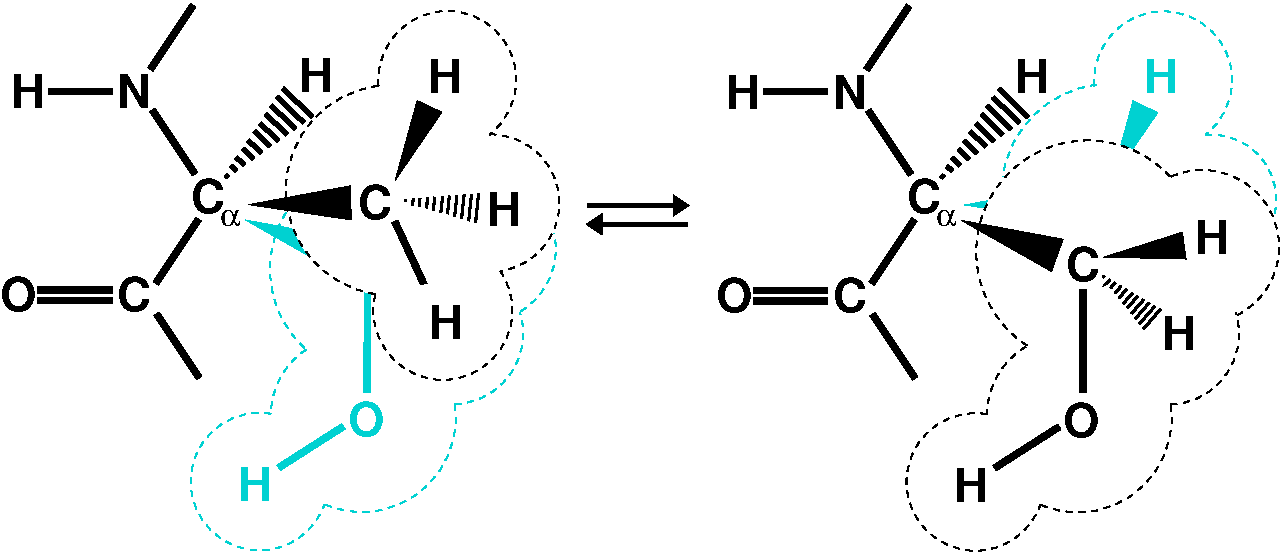
\includegraphics[width=12.5cm]{figures/dual_top}}
  \caption{Dual topology description for an alchemical simulation.
           Case example of the mutation of alanine into serine.
           The lighter color denotes the non--interacting, alternate
           state.
           \label{fig:dual_top}}
\end{figure}


The energy and forces are defined as a function of $\lambda$, in such a fashion
that the interaction of the methyl group of alanine with the rest of the
protein is effective at the beginning of the simulation, \ie~ $\lambda$ = 0,
while the glycine C$_\alpha$ hydrogen atom does not interact with the rest of
the protein, and {\it vice versa} at the end of the simulation, \ie~ $\lambda$
= 1. For intermediate values of $\lambda$, both the alanine and the glycine
side chains participate in nonbonded interactions with the rest of the protein,
scaled on the basis of the current value of $\lambda$. It should be clearly
understood that these side chains never interact with each other.


It is noteworthy that end points of alchemical transformations carried out in the framework of the dual--topology paradigm have been shown to be conducive to
numerical instabilities from molecular dynamics simulations, often coined as ``end--point
catastrophes''. These scenarios are prone to occur when $\lambda$ becomes close
to 0 or 1, and incoming atoms instantly appear where other particles are
already present, which results in a virtually infinite potential as the
interatomic distance tends towards 0. Such ``end--point catastrophes'' can be
profitably circumvented by introducing a so--called soft--core
potential~\cite{Beutler1994,Zacharias1994}, aimed at a gradual scaling of the short--range
nonbonded interactions of incoming atoms with their environment, as shown in Equation \ref{eqn:softcore}.  
What is really being modified is the value of a coupling parameter ($\lambda_\mathrm{LJ}$ or $\lambda_\mathrm{elec}$) that
scales the interactions --- \ie, if set to 0, the latter are off; if set to 1,
they are on --- in lieu of the actual value of $\lambda$ provided by the user.  

%CBH: TODO - SOFTCORE Eqn -- insert paragraph explanation ``What is softcore and what does it mean in NAMD2.7''.  Add softcore_lambda.png figure below softcore keywords in Implementation section
\begin{equation}
\label{eqn:softcore}
V_\mathrm{NB}(r_{ij}) = \lambda_\mathrm{LJ} \varepsilon_{ij} \left[ \left(\frac{R^\mathrm{min}_{ij}\,^2}{r_{ij}^2+\delta(1-\lambda_\mathrm{LJ})}\right)^{\!\!6}  -  \left(\frac{R^\mathrm{min}_{ij}\,^2}{r_{ij}^2+\delta(1-\lambda_\mathrm{LJ})}\right)^{\!\!3} \right]
+ \lambda_\mathrm{elec} \frac{q_iq_j}{\varepsilon_1 r_{ij}}
\end{equation}


It is also worth noting that the free energy calculation does not alter
intermolecular bonded potentials, \eg~bond stretch, valence angle deformation
and torsions, in the course of the simulation. In calculations targeted at the
estimation of free energy differences between two states characterized by
distinct environments --- \eg~a ligand, bound to a protein in the first
simulation, and solvated in water, in the second --- as is the case for most
free energy calculations that make use of a thermodynamic cycle, perturbation
of intramolecular terms may, by and large, be safely
avoided~\cite{Boresch1999}.  This property is controlled by the {\tt alchDecouple} keyword described in  



\subsubsection{Free Energy Perturbation}
\label{section:fepintro}


Within the FEP framework
~\cite{Beveridge1989,Chipot2002g,Chipot2007,Gilson1997,Kollman1993,Mark1998,Straatsma1992,VanGunsteren1989,Zwanzig1954},
the free energy difference between two
alternate states, $a$ and $b$, is expressed by:


\begin{equation}
\Delta A_{a \rightarrow b} = -\frac{1}{\beta} \ \ln
                              \left\langle \exp \left\{-\beta
                                                \left[{\cal H}_b({\bf x}, {\bf p}_x) -
                                                      {\cal H}_a({\bf x}, {\bf p}_x)
                                                \right]
                                                \right\}
                                                \right\rangle_a
\label{fep}
\end{equation}


\noindent Here, $\beta^{-1} \equiv k_B T$, where $k_B$ is the Boltzmann
constant, $T$ is the temperature. ${\cal H}_a({\bf x}, {\bf p}_x)$ and ${\cal
H}_b({\bf x}, {\bf p}_x)$ are the Hamiltonians describing states $a$ and $b$,
respectively. $\left\langle \cdots \right\rangle_a$ denotes an ensemble average
over configurations representative of the initial, reference state, $a$.


\begin{figure}[ht]
  \center{\vspace{0.4cm}
          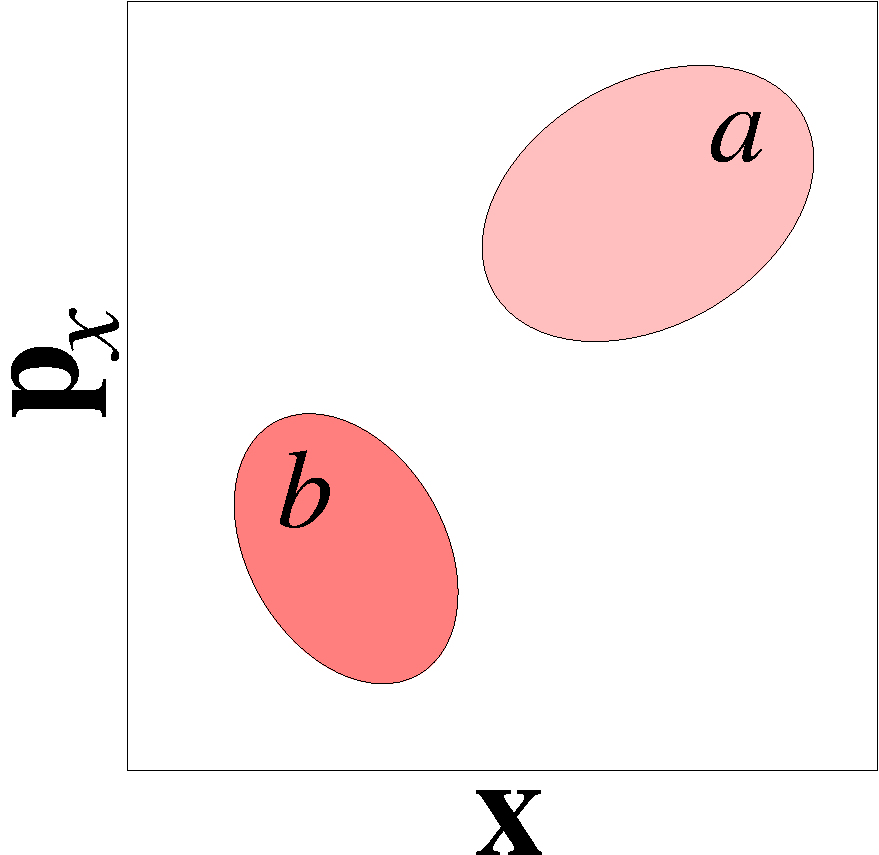
\includegraphics[width=4cm]{figures/overlap1}
          {\bfseries \sffamily (a)}
          \hfill
          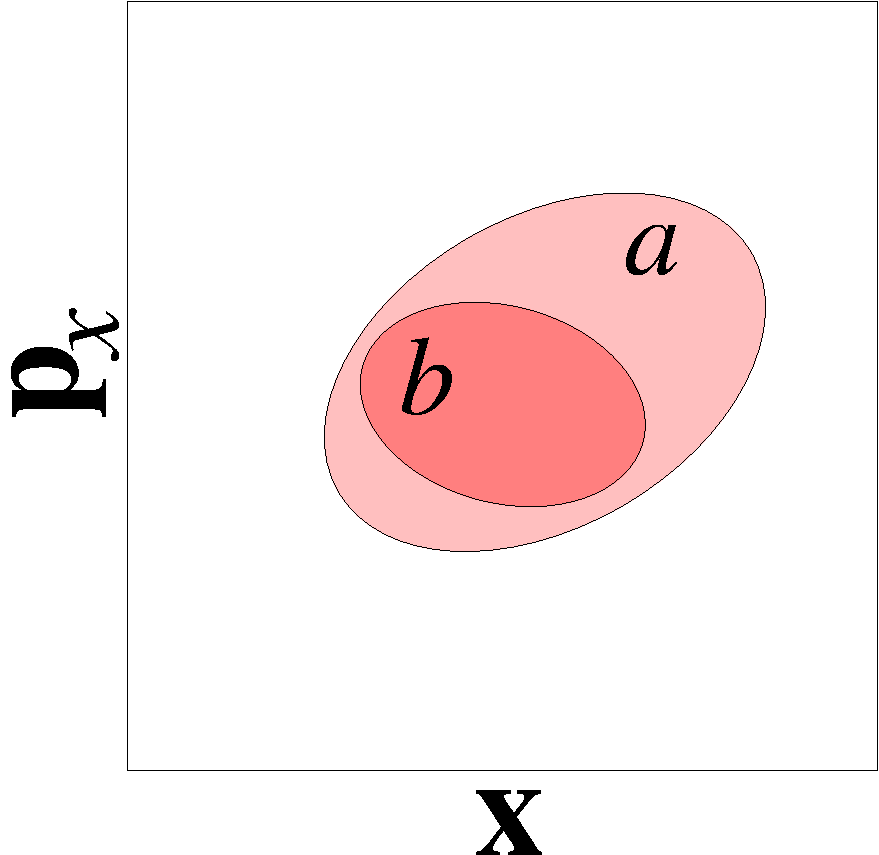
\includegraphics[width=4cm]{figures/overlap2}
          {\bfseries \sffamily (b)}
          \hfill
          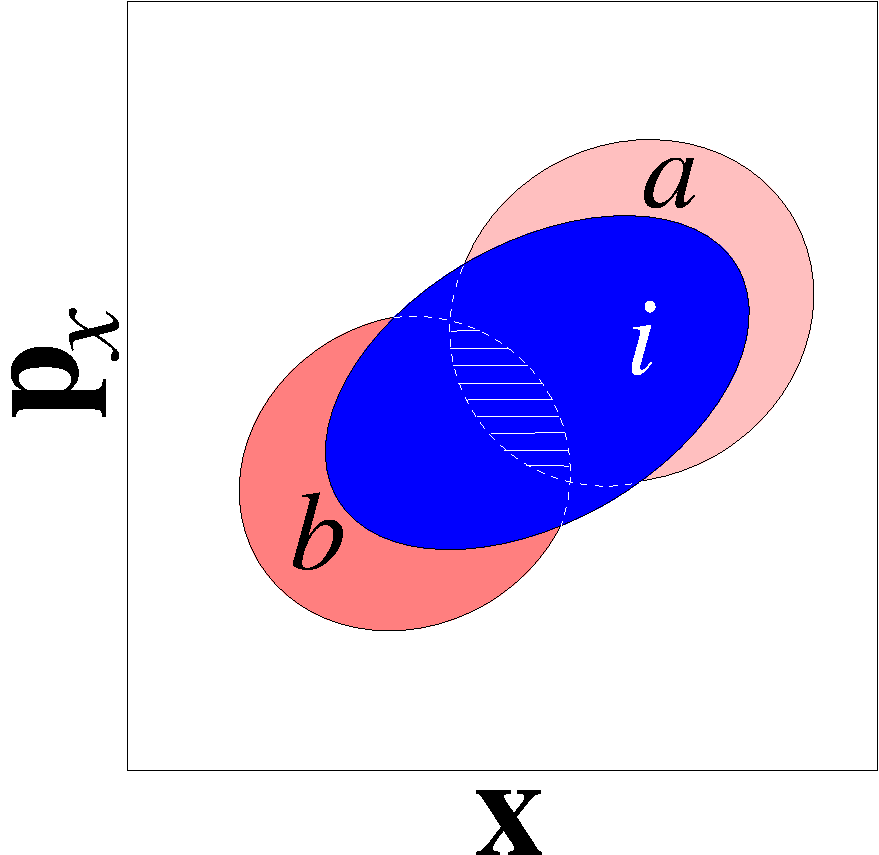
\includegraphics[width=4cm]{figures/overlap3}
          {\bfseries \sffamily (c)}}
  \caption{Convergence of an FEP calculation. If the ensembles representative
           of states $a$ and $b$ are too disparate, equation~({\ref{fep}}) will
           not converge {\bfseries \sffamily (a)}.
           If, in sharp contrast, the configurations of
           state $b$ form a subset of the ensemble of configurations
           characteristic of state $a$, the simulation is expected
           to converge {\bfseries \sffamily (b)}.
           The difficulties reflected in case {\bfseries \sffamily (a)} may be
           alleviated by the introduction of mutually overlapping intermediate
           states that connect $a$ to $b$ {\bfseries \sffamily (c)}. It should be
           mentioned that in practice, the kinetic contribution, ${\cal T}({\bf p}_x)$,
           is assumed to be identical for state $a$ and state $b$.
           \label{fig:overlap}}
\end{figure}


Convergence of equation~({\ref{fep}}) implies that low--energy configurations
of the target state, $b$, are also configurations of the reference state, $a$,
thus resulting in an appropriate overlap of the corresponding ensembles --- see
Figure~\ref{fig:overlap}.  Transformation between the two
thermodynamic states is replaced by a series of transformations between
non--physical, intermediate states along a well--delineated pathway that
connects $a$ to $b$. This pathway is characterized by the general extent
parameter ~\cite{Beveridge1989,King1993,Kirkwood1935,Mark1998}, $\lambda$, that
makes the Hamiltonian and, hence, the free energy, a continuous function of
this parameter between $a$ and $b$:


\begin{equation}
\Delta A_{a \rightarrow b} = -\frac{1}{\beta} \ \sum_{i = 1}^N \ln
                              \left\langle \exp\left\{-\beta
                                               \left[{\cal H}({\bf x}, {\bf p}_x; \lambda_{i+1}) -
                                                     {\cal H}({\bf x}, {\bf p}_x; \lambda_i)
                                               \right]
                                               \right\}
                                               \right\rangle_i
\label{windows}
\end{equation}


Here, $N$ stands for the number of intermediate stages, or ``windows''
between the initial and the final states --- see Figure~\ref{fig:overlap}.


\subsubsection{Thermodynamic Integration }

An alternative to the perturbation formula for free energy calculation is
Thermodynamic Integration (TI). With the TI method, the free energy is given
as~\cite{Kirkwood1935,Straatsma1991,Frenkel2002}:


\begin{equation}
\Delta A =  \int_0^1 \left<\frac{\partial
{\cal H}({\bf x}, {\bf p}_x; \lambda)}{\partial \lambda}\right>_\lambda d\lambda
\end{equation}


In the multi-configuration thermodynamic integration approach
~\cite{Straatsma1991} implemented in NAMD, $ \left<\partial {\cal H}({\bf x},
{\bf p}_x; \lambda) / \partial \lambda~\right>_\lambda $, the ensemble average
of the derivative of the internal energy with respect to $\lambda$, is
collected for a series of discrete $\lambda$ values and written to {\tt tiOutFile}. These values are analyzed by the separately distributed script
{\tt NAMD\_ti.pl}, which performs the integration of individual energy
components and reports back the total $\Delta A$ values for the transformation.



\subsection{Implementation of the free energy methods in NAMD}
\label{section:fepparameters}


The procedures implemented in NAMD are particularly
adapted for performing free
energy calculations that split the $\lambda$
reaction path into a number of non--physical,
intermediate states, or ``windows''. Separate simulations
can be started for each window.
Alternatively, the {\sc Tcl} scripting ability of
NAMD can be employed advantageously
to perform the complete simulation in a single run.
An example, making use of such a script, is supplied at the end
of this section.

The following keywords can be used to run alchemical free
energy calculations, whether FEP or TI.  
%Each keyword has two variants: one that is used in FEP calculations and a second that should be used when performing TI.  The FEP and TI variants are seperated by slashes like so: {\tt fepKeyword / tiKeyword}, listing first the FEP keyword and second the TI keyword. The FEP and TI specific keywords should be used exclusively with FEP or TI, respectively, and should not be intermixed during a simulation. 
%The attention of the user is directed to a novel hierarchy of parameters controlling both FEP and TI implementations.  Back-compatibility with configuration files running on previous versions of NAMD is nevertheless ensured by means of aliased commands.

\begin{itemize}
\item
\NAMDCONFWDEF{alch}{ Is an alchemical transformation to be performed? } {{\tt on} or {\tt off}} {{\tt off}} {Turns on alchemical transformation methods in NAMD.}
%\NAMDCONFWDEF{fep / thermInt}{ Is an alchemical free energy perturbation to be performed? } {{\tt on} or {\tt off}} {{\tt off}} {Turns on alchemical transformation methods in NAMD.}

\item
\NAMDCONFWDEF{alchType}{ Which method is to be employed for the alchemical transformation? } {{\tt fep} or {\tt ti}} {{\tt ti}} 
%if only {\tt alchLambda} is specified; {\tt fep} if {\tt alchLambdaPlusDelta} / {\tt alchLambdaMinusDelta} are specified} 
{Turns on Hamiltonian scaling and ensemble averaging for alchemical FEP or TI.}


\item
\NAMDCONF{alchLambda}{ Current value of the coupling parameter } {positive
decimal between 0.0 and 1.0} {The coupling parameter value determining the
progress of the perturbation for FEP or TI.}

\item
\NAMDCONF{alchLambda2}{Forward projected value of the coupling
parameter} {positive decimal between 0.0 and 1.0} {The {\tt
lambda2} value corresponds to the coupling parameter to be used for
sampling in the next window.  The free energy difference between {\tt
alchLambda2} and {\tt alchLambda} is calculated.  Through simulations
at progressive values of {\tt alchLambda} and {\tt alchLambda2} the
total free energy difference may be determined. }

%\item
%\NAMDCONF{alchLambdaMinusDelta}{Backward projected value of the coupling parameter} {positive decimal between 0.0 and 1.0} {The {\tt alchLambdaMinusDelta} value corresponds to the coupling parameter to be used for sampling in the previous window, assuming that a double-wide sampling simulation is being performed, whereby both the forward and the backward transformations are computed explicitly.  The free energy difference between {\tt alchLambdaMinusDelta} and {\tt alchLambda} is calculated.  Through simulations at progressive values of {\tt alchLambda} and {\tt alchLambdaMinusDelta} the total free energy difference may be determined.}

\item
\NAMDCONFWDEF{alchEquilSteps}{Number of equilibration steps in a window,
prior to data collection}
{positive integer less than {\tt numSteps} or {\tt run}}
{0}
{In each window {\tt alchEquilSteps} steps of equilibration can be
performed before ensemble averaging is initiated. The output also contains
the data gathered during equilibration and is meant for analysis of
convergence properties of the alchemical free energy calculation.}

\item
\NAMDCONFWDEF{alchFile}{{\tt pdb} file with perturbation flags}
{filename}
{coordinates}
{{\tt pdb} file to be used for indicating the status of all
atoms pertaining to the system, with respect to the alchemical transformation.
If this parameter is not declared specifically, then the
{\tt pdb} file specified by
{\tt coordinates} is utilized for this information.}

\item
\NAMDCONFWDEF{alchCol}{Column in the {\tt alchFile} that carries
                      the perturbation flag}
{X, Y, Z, O or B}
{B}
{Column of the {\tt pdb} file to use for retrieving the status
of each atom, \ie~a flag that indicates which atom will be perturbed
in the course of the alchemical transformation.
A value of {\tt -1} in the specified column indicates that the atom will
vanish as $\lambda$ moves from 0 to 1, whereas a value of {\tt 1}
indicates that it will grow.}

\item
\NAMDCONFWDEF{alchOutFreq}{Frequency of free energy output in time--steps}
{positive integer}
{5}
{Every {\tt alchOutFreq} number of MD steps, the output file
{\tt alchOutFile} is updated by dumping energies that are
used for ensemble averaging.
This variable could be set to {\tt 1} to include all the
configurations for ensemble averaging. Yet, it is recommended
to update {\tt alchOutFile}  energies at longer intervals
to avoid large files containing highly correlated data, unless a post--treatment,
\eg~Bennett's acceptance ratio (BAR)~\cite{Bennett1976} or simple overlap
sampling (SOS)~\cite{Lu2004}, is to be performed.}

\item
\NAMDCONFWDEF{alchOutFile}{Alchemical free energy output filename}
{filename}
{{\tt outfilename}}
{An output file named {\tt alchOutFile},
containing the FEP energies, or {\tt tiOutFile}, containing the TI derivatives, dumped every {\tt alchOutFreq} steps.}

\item
\NAMDCONFWDEF {alchVdwShiftCoeff}{Soft-core van der Waals radius-shifting coefficient}
{positive decimal}
{5} %CBH -- reconcile with SimParameters.C/.h
{This is a radius-shifting coefficient of $\lambda$ that is used
to construct the modified vdW interactions during alchemical free energy calculations.
Providing a positive value for {\tt alchVdWShiftCoeff} ensures that the vdW potential
is finite everywhere for small values of $\lambda$, which significantly improves the
accuracy and convergence of FEP and TI calculations, and also prevents overlapping particles
from making the simulation unstable. During FEP and TI, assuming $\lambda = 0$
denotes an absence of interaction, the interatomic distances used in
the Lennard-Jones potential are shifted according to ~\cite{Beutler1994,Zacharias1994}:
$r^2 \rightarrow r^2 + {\tt alchVdWShiftCoeff} \times (1 - \lambda)$
}

\item
\NAMDCONFWDEF {alchElecLambdaStart}{Value of $\lambda$ to introduce electrostatic interactions}
{positive decimal}
{0.5} %CBH -- reconcile with SimParameters.C/.h
{In order to avoid the so--called ``end-point catastrophes'', it is crucial to
avoid situations where growing particles overlap with existing particles with
an unbounded interaction potential, which would approach infinity as the
interaction distance approaches zero~\cite{Beutler1994,Chipot2007}. One possible route for
avoiding overlap of unbounded electrostatic potentials consists of allowing a
bounded (soft-core) vdW potential, using a positive value of {\tt
alchVdWShiftCoeff}, to repel first all overlapping particles at low values of
$\lambda$. As $\lambda$ increases, once the particles are repelled, it becomes
safe to turn on FEP or TI electrostatics. 

In the current implementation, the electrostatic interactions of an exnihilated, or appearing, particle are linearly coupled to the simulation over the $\lambda$ value range of {\tt alchElecLambdaStart} -- 1.0. At $\lambda$ values less than or equal to the user-defined value of {\tt alchElecLambdaStart}, electrostatic interactions of the exnihilated particle are fully decoupled from the simulation.  Coupling of electrostatic interactions then increases linearly for increasing values of $\lambda$ until $\lambda$=1.0, at which point electrostatic interactions of the exnihilated particle are fully coupled to the simulation.  

For annihilated, or vanishing, particles the electrostatic interactions are linearly decoupled from the simulation over the $\lambda$ value range of 0 -- (1.0 - {\tt alchElecLambdaStart}). At $\lambda$=0 electrostatic interactions are fully coupled to the simulation, and then linearly decreased with increasing $\lambda$ such that at $\lambda$ values greater than or equal to (1.0 - {\tt alchElecLambdaStart}) electrostatic interactions are completely decoupled from the simulation.  Two examples, shown in Figure \ref{fig:softcore}, describe the relationship between the user-defined value of $\lambda$ and the coupling of electrostatic or vdW interactions to the simulation. }

\begin{figure}
  \center{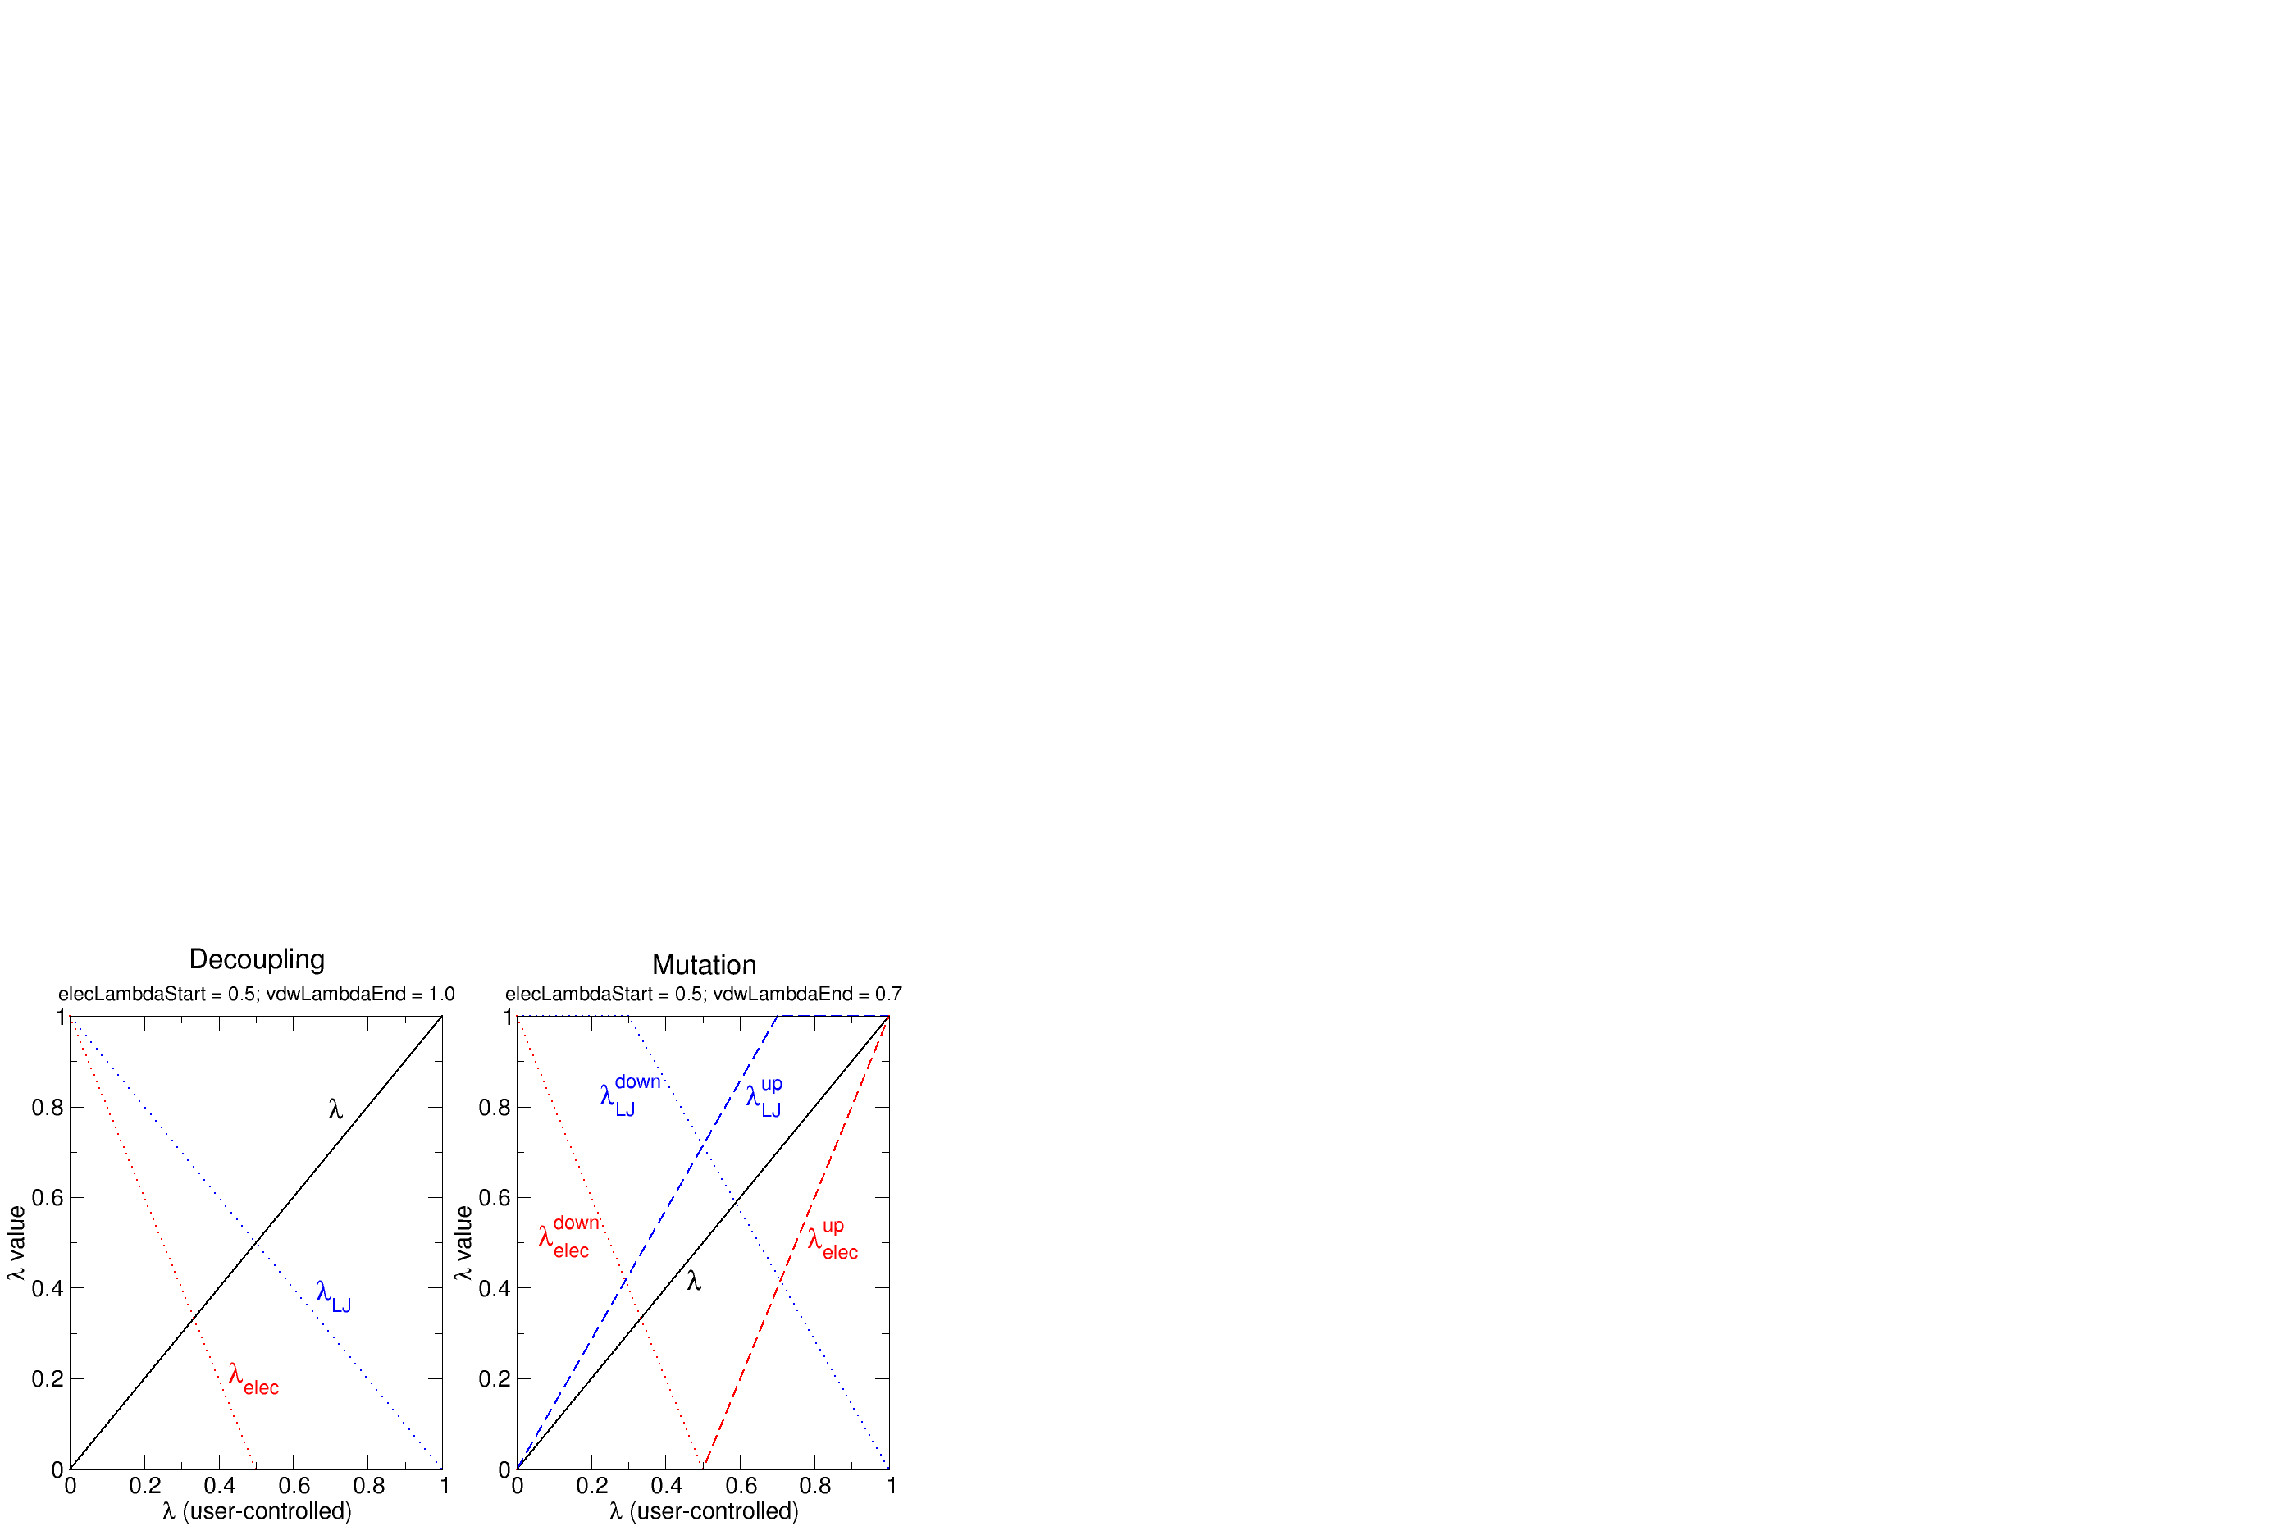
\includegraphics[width=0.75\textwidth]{figures/softcore_lambda}}
  \caption{Relationship of user-defined $\lambda$ to coupling of electrostatic or vdW interactions to a simulation, given specific values of {\tt alchElecLambdaStart} or {\tt alchVdwLambdaEnd}.}
  \label{fig:softcore}
\end{figure}

\item
  \NAMDCONFWDEF {alchVdwLambdaEnd}{Value of $\lambda$ to cancel van der Waals interactions}
{positive decimal}
{1.0} %CBH -- reconcile with SimParameters.C/.h
{If the {\tt alchElecLambdaStart} option is used, it may also be 
desirable to separate the scaling of van der Waals and electrostatic
interactions. {\tt alchVdwLambdaEnd} sets the value of $\lambda$ above which
all vdW interactions are fully enabled for exnihilated particles.

For an exnihilated particle, vdW interactions are fully decoupled at $\lambda$=0.  The coupling of vdW interactions to the simulation is then increased with increasing values of $\lambda$ such that at values of $\lambda$ greater than or equal to {\tt alchVdwLambdaEnd} the vdW interactions of the exnihilated particle are fully coupled to the simulation.

For an annihilated particle, vdW interactions are completely coupled to the simulation for $\lambda$ values between 0 and (1 - {\tt alchVdwLambdaEnd}). Then, vdW interactions of the annihilated particle are linearly decoupled over the range of $\lambda$ values between (1 - {\tt alchVdwLambdaEnd}) and 1.0. VdW interactions are only fully decoupled when $\lambda$ reaches 1.0.  
}





\item
  \NAMDCONFWDEF {alchDecouple}{Disable scaling of nonbonded interactions within alchemical partitions}
{{\tt on} or {\tt off}} {{\tt off}} {With {\tt alchDecouple} set to {\tt on},
only nonbonded interactions of perturbed, incoming and outgoing atoms with
their environment are scaled, while interactions within the subset of perturbed
atoms are preserved. On the contrary, if {\tt alchDecouple} is set to {\tt
off}, interactions within the perturbed subset of atoms are also scaled and
contribute to the cumulative free energy. In most calculations, intramolecular
annihilation free energies are not particularly informative, and decoupling
ought to be preferred. Under certain circumstances, it may, however, be
desirable to scale intramolecular interactions, provided that the latter are
appropriately accounted for in the thermodynamic cycle~\cite{Chipot2007}. }

%\item
%  \NAMDCONFWDEF {alchDoubleWideSampling}{Will an FEP alchemical transformation be performed in the forward and the backward directions concomitantly?} {{\tt on} or {\tt off}} {{\tt off}} %CBH -- reconcile with SimParameters.C/.h {Simultaneous alchemical transformations in the forward and the backward directions constitute a straightforward route towards the estimation of the error associated to the corresponding free energy calculations through their hysteresis. When set to {\tt on}, this option will request the concomitant evaluation of the ensemble averages over configurations representative of state $\lambda$, going (i) from $\lambda$ to $\lambda + \delta \lambda$ (controlled by keyword {\tt alchLambdaPlusDelta}), and  (ii) from $\lambda$ to $\lambda - \delta \lambda$ (controlled by keyword {\tt alchLambdaMinusDelta}). Accessing from a single free energy calculation the statistical information of both transformations is particularly useful for data post--processing, \eg~ BAR~\cite{Bennett1976} and SOS~\cite{Lu2004}, which have proven to improve the accuracy of the free--energy estimates over brute--force application of the FEP formula. It should be emphasized, however, that forward and backward transformations do not necessarily share the same convergence properties, so that, over finite--length simulations, free--energy differences will not be strictly equal.  } 

\end{itemize}



\subsection{Examples of input files for running alchemical free energy calculations}


The first example illustrates the use of {\sc Tcl} scripting for running
an alchemical transformation with the FEP feature of NAMD. In this
calculation, $\lambda$ is changed continuously from 0 to 1
by increments of $\delta \lambda$ = 0.1.


\begin{tabular}{ll}
\begin{minipage}{8cm}
\begin{verbatim}
alch           On
alchType       fep
alchFile       ion.fep
alchCol        X
alchOutfile    ion.fepout
alchOutFreq    5
alchEquilSteps 5000

set Lambda0    0.0
set dLambda    0.1

while {$Lambda0 < 1.0} {
 alchLambda $Lambda0
 set Lambda0 [expr $Lambda0 + $dLambda]
 alchLambda2 $Lambda0
 run  10000
}
\end{verbatim}
\end{minipage}
&
\begin{minipage}{7.8cm}
%\newline % LaTeX complains there is no line to end here
Enable alchemical simulation module
\newline
Set alchemical method to FEP
\newline
File containing the information about growing/shrinking atoms
described in column {\tt X}.
\newline
Output file containing the free energy.
\newline
Frequency at which {\tt fepOutFreq} is updated.
\newline
Number of equilibration steps per $\lambda$--state.
\\[0.6cm]
Starting value of $\lambda$.
\newline
Increment of $\lambda$, \ie~$\delta \lambda$.
\\[0.6cm]
{\sc Tcl} script to increment $\lambda$:
\newline
\hspace{0.4cm} (1) set {\tt lambda} value;
\newline
\hspace{0.4cm} (2) increment $\lambda$;
\newline
\hspace{0.4cm} (3) set {\tt lambda2} value;
\newline
\hspace{0.4cm} (4) run 10,000 MD steps.
\\
\end{minipage}
\end{tabular}


The user should be reminded that by setting {\tt run  10000},
10,000 MD steps will be performed, which includes the
preliminary {\tt fepEquilSteps} equilibration steps.
This means that here, the ensemble average of equation~({\ref{windows}})
will be computed  over 5,000 MD steps.


Alternatively, $\lambda$--states may be declared
explicitly, avoiding the use of {\sc Tcl} scripting:

\begin{tabular}{ll}
\begin{minipage}{8cm}
\begin{verbatim}
alchLambda      0.0
alchLambda2     0.1
run             10000
\end{verbatim}
\end{minipage}
&
\begin{minipage}{7.8cm}
(1) set {\tt alchLambda} value;
\newline
(2) set {\tt alchLambda2} value;
\newline
(3) run 10,000 MD steps.
\end{minipage}
\end{tabular}


This option is generally preferred to set up windows of diminishing
widths as $\lambda \rightarrow$ 0 or 1 --- a way to circumvent
end--point singularities caused by appearing atoms that may
clash with their surroundings.


The following second input is proposed for the measuring via TI the free energy
of a particle insertion.

\begin{verbatim}
    alch           On             ;# Enable alchemical simulation module
    alchType       ti             ;# Set method to thermodynamic integration
    alchFile       ion.alch.pdb   ;# PDB file with perturbation flags
    alchCol        B              ;# Perturbation flags in Beta column
    alchOutfile    ion.ti.out
    alchOutFreq    5
    alchEquilSteps 5000

    alchVdWShiftCoeff    1        ;# Enable soft-core vdW potential
    alchElecLambdaStart  0.1      ;# Introduce electrostatics for lambda > 0.1
    alchLambda 0
    run 10000
    alchLambda 0.00001
    run 10000
    alchLambda 0.0001
    run 10000
    alchLambda 0.001
    run 10000
    alchLambda 0.01
    run 10000

    set Lambda           0.1

    while {$Lambda <= 0.9} {
      alchLambda $Lambda
      run 10000
      set Lambda [expr $Lambda + 0.1]
    }

    alchLambda 0.99
    run 10000
    alchLambda 0.999
    run 10000
    alchLambda 0.9999
    run 10000
    alchLambda 0.99999
    run 10000
    alchLambda 1
    run 10000

\end{verbatim}

%In this example, most input parameters are shared with FEP, except for the specification of {\tt alchMethod ti} and the absence of {\tt alchLambdaPlusDelta} or {\tt alchLambdaMinusDelta} parameters. Moreover, 
Robust
sampling of the free energy of particle insertion is enabled by the use of
soft-core van der Waals scaling with the {\tt alchVdWShiftCoeff} parameter,
delayed introduction of electrostatics with a non-zero {\tt
alchElecLambdaStart} value, and very gradual scaling of $\lambda$ towards its
end points.



\subsection{Description of a free energy calculation output }


\subsubsection{Free Energy Perturbation }


When running FEP, the {\tt alchOutFile} contains electrostatic and van der Waals energy
data calculated for {\tt alchLambda} and {\tt alchLambda2}, written every
{\tt alchOutFreq} steps. The column {\tt dE} is the energy
difference of the single configuration, {\tt dE\_avg} and {\tt dG}
are the instantaneous ensemble average of the energy and the calculated
free energy at the time step specified in column 2, respectively.
The temperature is specified in the penultimate column. Upon completion
of {\tt alchEquilSteps} steps, the calculation of {\tt dE\_avg} and
{\tt dG} is restarted. The accumulated net free energy change is written
at each lambda value and at the end of the simulation.
%This will confuse people and doesn't apply with non-linear vdW scaling
%The cumulative average energy {\tt dE\_avg} value may be summed using the
%trapezoidal rule to obtain an approximate TI
%estimate for the free energy change during the run. =====> WHERE WILL IT CONFUSE PEOPLE?


Whereas the FEP module of NAMD supplies free energy differences determined from
equation~({\ref{fep}}), the wealth of information available in {\tt
alchOutFile} may be utilized profitably to explore different routes towards the
estimation of $\Delta A$. Both BAR and SOS methods, which combine
advantageously \emph{direct} and \emph{reverse} transformations to improve
convergence and accuracy of the calculation, represent relevant alternatives to
brute--force application of the FEP formula~\cite{Lu2004}.


Within the SOS framework, the free energy difference between states $\lambda_i$ and
$\lambda_{i+1}$ is expressed as:


\begin{equation}
\exp(-\beta \Delta A_{i \rightarrow i+1})  =
\frac{\displaystyle
      \left\langle \exp\left\{-\frac{\beta}{2}
                       \left[
                       {\cal H}({\bf x}, {\bf p}_x; \lambda_{i+1}) - {\cal H}({\bf x}, {\bf p}_x; \lambda_i)
                       \right]
                       \right\}
      \right\rangle_i}
      {\displaystyle
       \left\langle \exp\left\{-\frac{\beta}{2}
                       \left[
                       {\cal H}({\bf x}, {\bf p}_x; \lambda_i) - {\cal H}({\bf x}, {\bf p}_x; \lambda_{i+1})
                       \right]
                       \right\}
      \right\rangle_{i+1}}
\label{sos}
\end{equation}

\noindent and can be readily used with the statistical information provided by the forward and the backward runs.


\subsubsection{Thermodynamic Integration }


When running TI free energy calculations, the {\tt elec\_dU/dl} and {\tt
vdW\_dU/dl} values reported in {\tt tiOutFile} are the derivatives of the
internal energy with respect to $\lambda$ --- \ie~$\frac{\partial
U}{\partial\lambda}$ for electrostatics and, van der Waals, respectively. {\tt
dU/dl} values are averages over the last {\tt tiOutFreq} steps. Cumulative
averages for each component are reported alongside in the {\tt \_avg} columns.


The electrostatics and vdW are separated following a partition scheme --- that
is, the ``appearing'' and the ``disappearing'' atoms are accounted for
separately. ``Partition 1'' contains those atoms whose interactions are
switched up as $\lambda$ increases --- \ie~flagged with {\tt 1} in the {\tt
alchFile}. ``Partition 2'' represents those atoms whose interactions are
switched down as $\lambda$ increases --- \ie~flagged with {\tt -1}. $\Delta A$
values for each component are obtained by integrating from $\lambda=0$ to $1$
using the respective {\tt ELEC / VDW LAMBDA} listed for each partition after
the title.


Analysis is handled by the {\tt NAMD\_ti} script, available from
\begin{quote}
http://www.ks.uiuc.edu/Research/namd/utilities/
\end{quote}


Although the output format of {\tt NAMD\_ti.pl } may appear to lend itself easily to interpretation of the
individual contributions to the free energy total (elec and vdW for each partition), this is rarely
appropriate as these values are path-dependent. For example, an output such as


\begin{verbatim}
          |-----------------------------------------------|
          |         |    elec   |    vdW    |   Subtotal  |
          |-----------------------------------------------|
          | Part. 1 |   -0.5748 |   -6.3452 |    -6.9200  |
          | Part. 2 |    0.5391 |    4.9387 |     5.4778  |
          |-----------------------------------------------|
          | Subtotal|    0.6048 |    0.3293 |   -12.3978  |
          |-----------------------------------------------|
          Total deltaG for transition lambda 0 -> 1: -12.3978
\end{verbatim}


\noindent may encourage interpretations along the lines of "the free energy for
switching on the van der Waals interactions for the atoms of partition 1 was
-6.35kcal/mol". This is only correct in the very narrow context of the
simulation setup and parameters used in this case and is not informative in a
broader sense.


%\begin{figure}[ht]
\begin{figure}
  \center{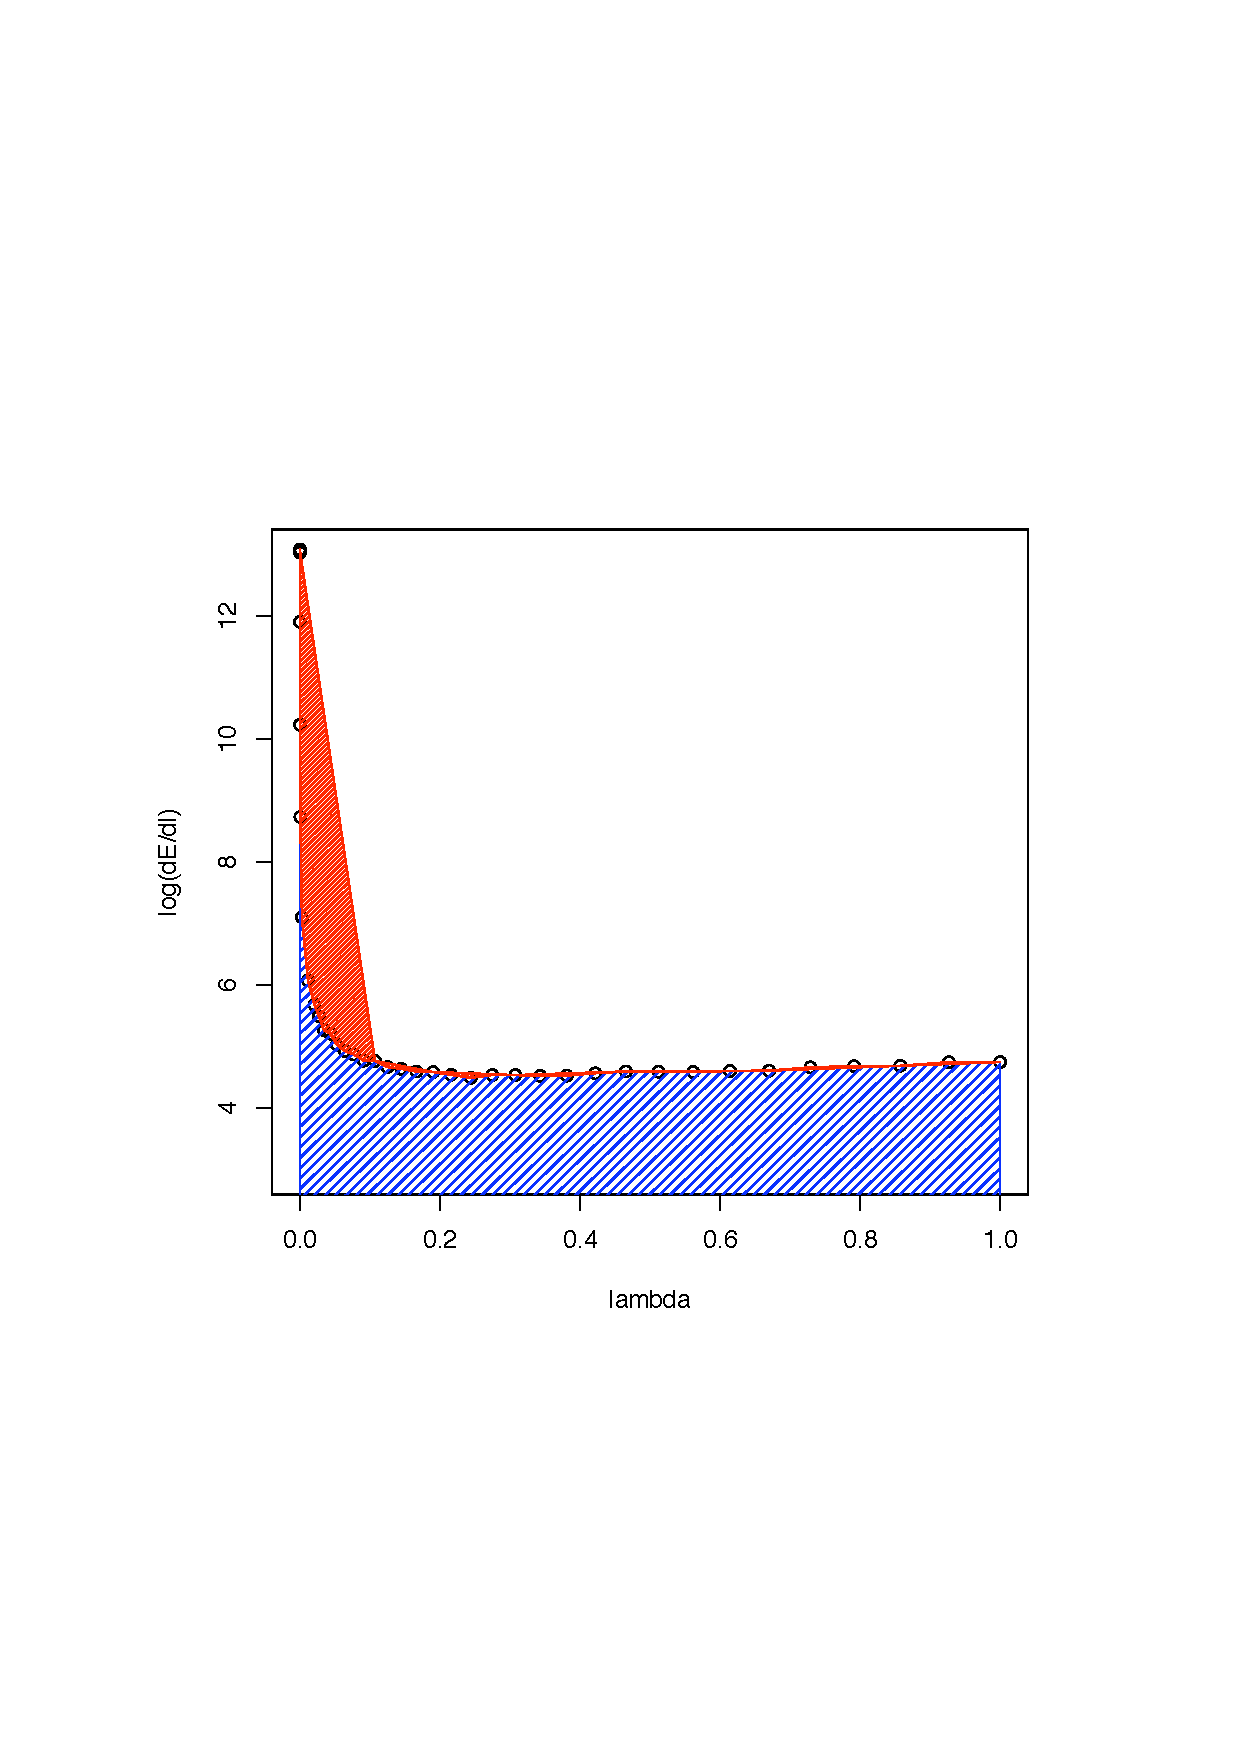
\includegraphics[width=0.75\textwidth]{figures/TI}}
  \caption{Sample TI data ($log(\left<\frac{\partial U}{\partial\lambda}\right>)$ against $\lambda$). The blue shaded
  area shows the integral with fine sampling close to the end point. The red area
  shows the difference when $\lambda$ values are more sparse. In this example,
  insufficient sampling before $\lambda$ $\simeq$0.1 can result in a large overestimation
  of the integral. Beyond $\simeq$0.2, sparser sampling is justified as dE/d$\lambda$ is not
  changing quickly.}
  \label{fig:TI}
\end{figure}


The choice of $\lambda$ values will depend on the application, but in general
it is important to examine the shape of the curve to ensure that sampling is
adequate to give a good estimate of the integral. In particular, it will be
necessary to sample more finely towards the end points in order to accurately
account for the strong repulsive van der Waals forces encountered when
inserting particles into a system (see Figure~\ref{fig:TI}).



%\bibliographystyle{unsrt}
%\bibliography{ug}
%\bibliography{../../LaTeX/Bibliography/data_base}

%\end{document}


% Accelerated sampling methods
\newpage
\section{Accelerated Sampling Methods}
\label{section:accel}

\subsection{Accelerated Molecular Dynamics}
\label{section:accelmd}
Accelerated molecular dynamics (aMD)~\cite{HAME2004mc} is an enhanced-sampling method that
improves the conformational space sampling by 
reducing energy barriers separating different states of a system.
The method modifies the potential 
energy landscape by raising energy wells that are below
a certain threshold level, while leaving those above this level unaffected.
As a result, barriers separating adjacent energy basins are reduced, allowing the system to sample
conformational space that cannot be easily accessed in a classical MD simulation.

Please include the following two references in your work using the NAMD implementation of aMD:
\begin{itemize}
  \item {Accelerated Molecular Dynamics: A Promising and Efficient Simulation Method for Biomolecules, D.\,Hamelberg, J.\,Mongan, and J.\,A. McCammon. {\it J. Chem. Phys.}, 120:11919-11929, 2004.}
  \item{Implementation of Accelerated Molecular Dynamics in NAMD, Y.\,Wang, C.\,Harrison, K.\,Schulten, and J.\,A. McCammon, {\it Comp.~Sci.~Discov.}, 4:015002, 2011.}
\end{itemize}

\subsubsection{Theoretical background}
In the original form of aMD~\cite{HAME2004mc}, when the system's potential energy falls       
below a threshold energy, $E$, a boost potential is added, 
such that the modified potential, $V^*({\bf r})$, is related to the original
potential, $V({\bf r})$, via
\begin{equation}
V^*({\bf r})= V({\bf r}) + \Delta V({\bf r}),
\end{equation}
where $\Delta V({\bf r})$ is the boost potential, 
\begin{equation} 
\Delta V({\bf r})= \left \{
\begin{array}{l l}
0   & \quad \quad V({\bf r})\geq E \\  
\frac{(E-V({\bf r}))^2}{\alpha+E-V({\bf r})}  & \quad \quad V({\bf r})<E. \\
\end{array} \right. 
\end{equation}
As shown in the following figure, the threshold energy $E$ controls the portion of 
the potential surface affected by the boost, while the acceleration factor 
$\alpha$ determines the shape of the modified potential.
%as $\alpha$ increases, the modified potential asymptotically approaches the original potential;
%as $\alpha$ decreases, the energy surface below $E$ begins to resemble a constant potential.
Note that $\alpha$ cannot be set to zero, otherwise the derivative of the modified potential
is discontinuous.

\begin{figure}[!ht]
  \centering
  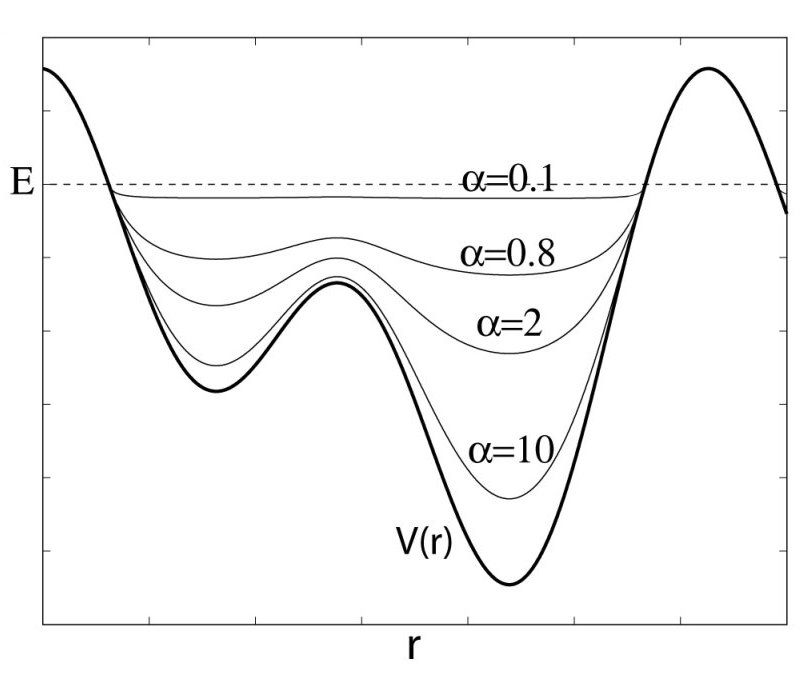
\includegraphics[width=7cm]{figures/amd_schematic.jpg}
  \caption{Schematics of the aMD method. When the original potential (thick line) falls below a threshold energy $E$ (dashed line),
          a boost potential is added. The modified energy profiles (thin lines) have smaller barriers separating adjacent
	  energy basins. 
	  %Two parameters, $E$ and $\alpha$, controls the portion of the affected potential landscape and the
	  %shape of the modified potential, respectively.
	  }
  \label{fig:amd_schematic}
\end{figure}
From an aMD simulation, the ensemble average, $\langle A \rangle$, of an observable, $A({\bf r})$, can be calculated
using the following reweighting procedure:
\begin{equation}
\langle A \rangle =\frac{\langle A({\bf r})\,\text{exp} (\beta \Delta V({\bf r})) \rangle^* }
{\langle \text{exp}  (\beta \Delta V({\bf r})) \rangle^*},
\end{equation}
in which $\beta$=$1/k_BT$, and $\langle ... \rangle$ and $\langle...\rangle^*$ represent 
the ensemble average in the original and the aMD ensembles, respectively. 

Currently, aMD can be applied in three modes in NAMD: aMDd, aMDT, and aMDdual~\cite{WANG2011mc}. The boost energy
is applied to the dihedral potential in the aMDd mode (the default mode), and to the total potential in the aMDT mode.
In the dual boost mode (aMDdual)~\cite{HAME2007mc}, two independent boost energies are applied, one on the dihedral potential and the other
on the (Total - Dihedral) potential.

\subsubsection{NAMD parameters}

The following parameters are used to enable accelerated MD:

\begin{itemize}

\item
\NAMDCONFWDEF{accelMD}{Is accelerated molecular dynamics active?}{{\tt on} or {\tt
off}}{{\tt off}}
{Specifies if accelerated MD is active.}

\item
\NAMDCONFWDEF{accelMDdihe}{Apply boost to dihedrals?}{{\tt on} or {\tt off}} {{\tt on}} 
{Only applies boost to the dihedral potential. 
By default, {\tt accelMDdihe} is turned on and the boost energy is applied to the dihedral potential of the simulated system.
When {\tt accelMDdihe} is turned off, aMD switches to the {\tt accelMDT} mode, and the boost is applied to the total potential.
}

\item
\NAMDCONF{accelMDE}{Threshold energy $E$}
{Real number}
{Specifies the threshold energy $E$ in the aMD equations. 
}

\item
\NAMDCONF{accelMDalpha}{Acceleration factor $\alpha$}
{Positive real number}
{Specifies the acceleration factor $\alpha$ in the aMD equations. 
}

\item
\NAMDCONFWDEF{accelMDdual}{Use dual boost mode?}{{\tt on} or {\tt off}}{{\tt off}}
{When {\tt accelMDdual} is on, aMD switches to the dual boost mode. Two independent boost potentials 
will be applied: one to the dihedral potential that is controlled by the parameters {\tt accelMDE} and {\tt accelMDalpha},
and a second to the (Total - Dihedral) potential that is controlled by the  {\tt accelMDTE} and {\tt accelMDTalpha} parameters described below.
}

\item
\NAMDCONF{accelMDTE}{Threshold energy $E$ in the dual boost mode}
{Real number}
{Specifies the threshold energy $E$ used in the calculation of boost energy for the (Total - Dihedral) potential. 
This option is only available when {\tt accelMDdual} is turned on.
}

\item
\NAMDCONF{accelMDTalpha}{Acceleration factor $\alpha$ in the dual boost mode}
{Positive real number}
{Specifies the acceleration factor $\alpha$ used in the calculation of boost energy for the (Total - Dihedral) potential. 
This option is only available when {\tt accelMDdual} is turned on.
}

\item
\NAMDCONFWDEF{accelMDFirstStep}{First accelerated MD step}
{Zero or positive integer}{0}
{Accelerated MD will only be performed when the current step is equal to or higher than {\tt accelMDFirstStep}, and equal to or lower than {\tt accelMDLastStep}. Otherwise regular MD will be performed.
}
\item
\NAMDCONFWDEF{accelMDLastStep}{Last accelerated MD step}
{Zero or positive integer}{0}
{Accelerated MD will only be performed when the current step is equal to or higher than {\tt accelMDFirstStep}, and equal to or lower than {\tt accelMDLastStep}. Otherwise regular MD will be performed. Note that the accelMDLastStep parameter only has an effect when it is positive. When accelMDLastStep is set to zero (the default), aMD is `open-ended' and will be performed
till the end of the simulation. 
}

\item
\NAMDCONFWDEF{accelMDOutFreq}{Frequency in steps of aMD output}
{Positive integer}{1}
{An aMD output line will be printed to the log file at the frequency specified by {\tt accelMDOutFreq}.
The aMD output will contain the boost potential ($dV$) at the current timestep, 
the average boost potential ($dVAVG$) since the last aMD output, and various potential energy values at the current timestep.
The boost potential $dV$ can be used to reconstruct the ensemble average described earlier.
}

\end{itemize}

\subsection{Adaptive Tempering}
\label{section:adapttemp}
Adaptive tempering is akin to a single-copy replica exchange method for dynamically updating the simulation temperature. The temperature $T$ is a new random variable in the range $[Tmin,Tmax]$ that is governed by the equation $dE/dT = E-E(T)-1/T+sqrt(2)T\xi$, where $\xi$ is Gaussian white noise. The effect is that when the potential energy for a given structure is lower than the (so far calculated) average energy, the temperature is lowered. Conversely when the current energy is higher than the average energy, the temperature is raised. The effect is faster conformational sampling to find minimum energy structures. The method is implemented exactly as described by Zhang and Ma in J. Chem. Phys. 132, 244101 (2010) (using Equation 18 of their paper to calculate the average energy at a given temperature from the histogram of energies). 

The dynamic temperature is realized either by changing the temperature of the Langevin thermostat or by velocity rescaling. 

\subsubsection{NAMD parameters}

The following parameters are used to adaptive tempering:

\begin{itemize}

\item
\NAMDCONFWDEF{adaptTempMD}{Is adaptive tempering active?}{{\tt on} or {\tt
off}}{{\tt off}}
{Specifies whether or not adaptive tempering is used. If set to on then the following parameters are required to be set: either all of ({\tt adaptTempTmin}, {\tt adaptTempTmax}, {\tt adaptTempBins}, {\tt adaptTempDt}) or {\tt adaptTempInFile} (but not both).
}

\item
\NAMDCONFWDEF{adaptTempFreq}{steps between temperature updates}
{Positive integers}{10}
{The number of steps between temperature updates. Note that the potential energy at the current is calculated and added to the temperature-energy histogram at every step.
}

\item
\NAMDCONF{adaptTempTmin}{minimum temperature (K)}
{Positive real number} 
{Sets the minimum temperature to be used in the simulation.
}

\item
\NAMDCONF{adaptTempTmax}{maximum temperature (K)}
{Positive real number}
{Sets the maximum temperature to be used in the simulation.
}

\item
\NAMDCONFWDEF{adaptTempBins}{number of temperature bins}
{Positive integer}{1000}
{Sets the number of bins to subdivide the temperature range. Each bin stores the average energy for the given temperature 
}

\item
\NAMDCONFWDEF{adaptTempDt}{stepsize for temperature updates}{Positive real numbers}{$10^{-4}$}
{Integration timestep for temperature updates. This is unrelated to the simulation timestep and only scales the size of the step taken in temperature space every {\tt adaptTempFreq} steps.
}

\item
\NAMDCONF{adaptTempInFile}{adaptive tempering input filename}
{UNIX filename}
{The input file containing restart information for adaptive tempering (written out by {\tt adaptTempRestartFile}).
}

\item
\NAMDCONF{adaptTempRestartFile}{adaptive tempering restart filename}
{UNIX filename}
{The file to write out restart information for adaptive tempering.
}

\item
\NAMDCONF{adaptTempRestartFreq}{steps between writing restart file}
{Positive integer}
{Frequency of writing restart file.
}

\item
\NAMDCONFWDEF{adaptTempLangevin}{send temperature updates to langevin thermostat?}
{{\tt on} or {\tt off}}{{\tt on}}
{Setting this to on will cause the langevin thermostat to use the updated temperatures from adaptive tempering. Note that either one of adaptTempLangevin or adaptTempRescaling have to be on.
}

\item
\NAMDCONFWDEF{adaptTempRescaling}{send temperature to velocity rescaling thermostat?}
{{\tt on} or {\tt off}}{{\tt on}}
{Setting this to on will cause the veloctiy rescaling thermostat to use the updated temperatures from adaptive tempering.  Note that either one of adaptTempLangevin or adaptTempRescaling have to be on.
}

\item
\NAMDCONFWDEF{adaptTempOutFreq}{steps between printing adaptive tempering output}
{Positive integers}{10}
{The number of timesteps between printing adaptive tempering output to the log file.
}

\item
\NAMDCONFWDEF{adaptTempFirstStep}{step to start adaptive tempering}
{Non-negative integers}{0}
{The first timestep from which adaptive tempering will be run.}

\item
\NAMDCONF{adaptTempLastStep}{step to stop adaptive tempering}
{Positive integers}
{The last timestep to apply adaptive tempering.}

\item
\NAMDCONFWDEF{adaptTempCgamma}{dynamic bin averaging constant}
{Non-negative real number}{0.1}
{The calculation of the mean energy for a given bin is weighted by a factor of 1 - Cgamma / samples to damp out old statistics. Setting Cgamma to zero restores the use of a standard arithmetic mean to calculate the mean energy for each bin.}

\item
\NAMDCONFWDEF{adaptTempRandom}{assign random temperature if we step out of range?}
{{\tt on} or {\tt off}}{{\tt off}}
{If set to on and the temperature steps out of [{\tt adaptTempTmin}, {\tt adaptTempTmax}], a random temperature in that range is assigned. Otherwise the previous temperature is kept.
}

%\item
%\NAMDCONFWDEF{adaptTempDebug}{print debug output?}
%{{\tt on} or {\tt off}}{{\tt off}}
%{Print adaptive tempering debug output.
%}

\end{itemize}


\subsection{Locally enhanced sampling}
\label{section:les}

Locally enhanced sampling (LES)~\cite{ROIT91,SIMM98,SIMM00} increases
sampling and transition rates for a portion of a molecule by the use of
multiple non-interacting copies of the enhanced atoms.  These enhanced
atoms experience an interaction (electrostatics, van der Waals, and
covalent) potential that is divided by the number of copies present.
In this way the enhanced atoms can occupy the same space, while the
multiple instances and reduces barriers increase transition rates.

\subsubsection{Structure generation}

To use LES, the structure and coordinate input files must be modified to
contain multiple copies of the enhanced atoms.  \PSFGEN\ provides the
{\tt multiply} command for this purpose.  \NAMD\ supports a maximum of 255
copies, which should be sufficient.  

Begin by generating the complete molecular structure and guessing
coordinates as described in Sec.~\ref{section:psfgen}.  As the last
operation in your script, prior to writing the psf and pdb files, add
the {\tt multiply} command, specifying the number of copies desired and
listing segments, residues, or atoms to be multiplied.  For example,
\verb#multiply 4 BPTI:56 BPTI:57# will create four copies of the last
two residues of segment BPTI.  You must include all atoms to be
enhanced in a single {\tt multiply} command in order for the bonded
terms in the psf file to be duplicated correctly.  Calling {\tt multiply}
on connected sets of atoms multiple times will produce unpredictable
results, as may running other commands after {\tt multiply}.

The enhanced atoms are duplicated exactly in the structure---they have
the same segment, residue, and atom names.  They are distinguished only
by the value of the B (beta) column in the pdb file, which is 0 for
normal atoms and varies from 1 to the number of copies created for
enhanced atoms.  The enhanced atoms may be easily observed in VMD with
the atom selection \verb#beta != 0#.

\subsubsection{Simulation}

In practice, LES is a simple method used to increase sampling;
no special output is generated.
The following parameters are used to enable LES:

\begin{itemize}

\item
\NAMDCONFWDEF{les}{is locally enhanced sampling active?}{{\tt on} or {\tt
off}}{{\tt off}}
{Specifies whether or not LES is active.}

\NAMDCONF{lesFactor}{number of LES images to use}
{positive integer equal to the number of images present}
{This should be equal to the factor used in {\tt multiply}
 when creating the structure.  The interaction potentials for images is
 divided by {\tt lesFactor}.  
}

\item
\NAMDCONFWDEF{lesReduceTemp}{reduce enhanced atom temperature?}{{\tt on} or {\tt
off}}{{\tt off}}
{Enhanced atoms experience interaction potentials divided by {\tt lesFactor}.
This allows them to enter regions that would not normally be thermally
accessible.  If this is not desired, then the temperature of these atoms
may be reduced to correspond with the reduced potential.  This option
affects velocity initialization, reinititialization, reassignment, and
the target temperature for langevin dynamics.  Langevin dynamics is
recommended with this option, since in a constant energy simulation energy
will flow into the enhanced degrees of freedom until they reach thermal
equilibrium with the rest of the system.  The reduced temperature atoms
will have reduced velocities as well, unless {\tt lesReduceMass} is also
enabled.}

\item
\NAMDCONFWDEF{lesReduceMass}{reduce enhanced atom mass?}{{\tt on} or {\tt off}}{{\tt off}}
{Used with {\tt lesReduceTemp} to restore velocity distribution to
enhanced atoms.  If used alone, enhanced atoms would move faster than
normal atoms, and hence a smaller timestep would be required.}

\item
\NAMDCONFWDEF{lesFile}{PDB file containing LES flags}{UNIX filename} {{\tt coordinates}}
{PDB file to specify the LES image number of each atom.
If this parameter is not specified, then 
the PDB file containing initial coordinates specified by 
{\tt coordinates} is used.}

\item
\NAMDCONFWDEF{lesCol}{column of PDB file containing LES flags}{{\tt X}, {\tt Y}, {\tt Z}, {\tt O}, or {\tt B}}{{\tt B}}
{Column of the PDB file to specify the LES image number of each atom.
This parameter may specify any of the floating point fields of the PDB file, 
either X, Y, Z, occupancy, or beta-coupling (temperature-coupling).  
A value of 0 in this column indicates that the atom is not enhanced.
Any other value should be a positive integer less than {\tt lesFactor}.}

\end{itemize}


\subsection{Replica exchange simulations}

\index{replica exchange}
The {\tt lib/replica/}
directory contains Tcl scripts that implement replica exchange
both for parallel tempering (temperature exchange) and
umbrella sampling (exchanging collective variable biases).
This replaces the old Tcl server and socket connections driving a
separate NAMD process for every replica used in the simulation.

{\bf A NAMD build based on Charm++ 6.5.0 or later using one of the
``LRTS'' (low-level runtime system) machine layers is required!}
Current LRTS machine layers include
gemini\_gni-crayxe, pamilrts-bluegeneq, and mpi.

Only temperature-exchange simulations are described below.
To employ replicas for umbrella sampling you will need to understand
this material, collective variable-based calculations (Sec.\ \ref{section:colvars}),
and basic Tcl programming to adapt the examples in {\tt lib/replica/umbrella/}
and {\tt lib/replica/umbrella2d/} until further
documentation and a tutorial are available.

This implementation is designed to be modified to implement
exchanges of parameters other than temperature or via other temperature
exchange methods.  The scripts should provide a good starting point for
any simulation method requiring a number of loosely interacting systems.

Replica exchanges and energies are recorded in the .history files
written in the output directories.  These can be viewed with, e.g.,
``{\tt xmgrace output/*/*.history}'' and processed via awk or other tools.
There is also a script to load the output into VMD and color each
frame according to replica index.  An example simulation folds
a 66-atom model of a deca-alanine helix in about 10\,ns.

{\tt replica.namd}
is the master script for replica temperature-exchange simulations.  To run:
\begin{verbatim}
          cd example
          mkdir output
          (cd output; mkdir 0 1 2 3 4 5 6 7)
          mpirun namd2 +replicas 8 job0.conf +stdout output/%d/job0.%d.log
          mpirun namd2 +replicas 8 job1.conf +stdout output/%d/job1.%d.log
\end{verbatim}

The number of MPI ranks must be a multiple of the number of replicas
(+replicas).  Be sure to increment jobX for +stdout option on command line.

{\tt show\_replicas.vmd} is a script for loading replicas into VMD;
first source the replica exchange conf file and then this script, then
repeat for each restart conf file or for example just do
``{\tt vmd -e load\_all.vmd}''.
This script will likely destroy anything else you are doing in VMD at the
time, so it is best to start with a fresh VMD.
{\tt clone\_reps.vmd} provides the {\tt clone\_reps} commmand to copy graphical
representation from the top molecule to all other molecules.

{\tt sortreplicas}, found in the namd2 binary directory, is a program to un-shuffle
replica trajectories to place same-temperature frames in the same file.
Usage:
\begin{verbatim}
  sortreplicas <job_output_root> <num_replicas> <runs_per_frame> [final_step]
\end{verbatim}
where job\_output\_root is the job specific output base path, including
\%s or \%d for separate directories as in output/\%s/fold\_alanin.job1
This will be extended with .\%d.dcd .\%d.history for input files and
.\%d.sort.dcd .\%d.sort.history for output files.  The optional final\_step
parameter will truncate all output files after the specified step,
which is useful in dealing with restarts from runs that did not complete.
Colvars trajectory files are similarly processed if they are found.

A replica exchange config file should define the following Tcl variables:
\begin{itemize}
\item {\tt num\_replicas}, the number of replica simulations to use,
\item {\tt min\_temp}, the lowest replica target temperature,
\item {\tt max\_temp}, the highest replica target temperature,
\item {\tt steps\_per\_run}, the number of steps between exchange attempts,
\item {\tt num\_runs}, the number of runs before stopping
(should be divisible by {\tt runs\_per\_frame} $\times$ {\tt frames\_per\_restart}).
\item {\tt runs\_per\_frame}, the number of runs between trajectory outputs,
\item {\tt frames\_per\_restart}, the number of frames between restart outputs,

\item {\tt namd\_config\_file}, the NAMD config file containing all parameters,
needed for the simulation except {\tt seed}, {\tt langevin}, 
{\tt langevinTemp}, {\tt outputEnergies},
{\tt outputname}, {\tt dcdFreq},
{\tt temperature}, {\tt bincoordinates}, {\tt binvelocities},
or {\tt extendedSystem}, which are provided by {\tt replica.namd},

\item {\tt output\_root}, the directory/fileroot for output files,
optionally including a ``\%s'' that is replaced with the replica index
to use multiple output directories,

\item {\tt psf\_file}, the psf file for {\tt show\_replicas.vmd}, 
\item {\tt initial\_pdb\_file}, the initial coordinate pdb file for {\tt show\_replicas.vmd},
\item {\tt fit\_pdb\_file}, the coodinates that frames are fit to by {\tt show\_replicas.vmd} (e.g., a folded structure),
\end{itemize}

The {\tt lib/replica/example/} directory contains
all files needed to fold a 66-atom model of a deca-alanine helix:
\begin{itemize}
\item {\tt alanin\_base.namd}, basic config options for NAMD,
\item {\tt alanin.params}, parameters,
\item {\tt alanin.psf}, structure,
\item {\tt unfolded.pdb}, initial coordinates,
\item {\tt alanin.pdb}, folded structure for fitting in {\tt show\_replicas.vmd},
\item {\tt fold\_alanin.conf}, config file for {\tt replica\_exchange.tcl} script,
\item {\tt job0.conf}, config file to start alanin folding for 10\,ns,
\item {\tt job1.conf}, config file to continue alanin folding another 10\,ns, and
\item {\tt load\_all.vmd}, load all output into VMD and color by replica index.
\end{itemize}

The {\tt fold\_alanin.conf} config file contains the following settings:
\begin{verbatim}
set num_replicas 8
set min_temp 300
set max_temp 600
set steps_per_run 1000
set num_runs 10000
# num_runs should be divisible by runs_per_frame * frames_per_restart
set runs_per_frame 10
set frames_per_restart 10
set namd_config_file "alanin_base.namd"
set output_root "output/%s/fold_alanin" ; # directories must exist

# the following used only by show_replicas.vmd
set psf_file "alanin.psf"
set initial_pdb_file "unfolded.pdb"
set fit_pdb_file "alanin.pdb"
\end{verbatim}

\subsection{Random acceleration molecular dynamics simulations}

The "lib/ramd" directory stores the tcl scripts and the example files for the implementation of the Random Acceleration Molecular Dynamics (RAMD) simulation method in NAMD. 
The RAMD method can be used to carry out molecular dynamics (MD) simulations with an additional randomly oriented acceleration applied to the center of mass of one group of atoms (referred below as "ligand") in the system. 
It can, for example, be used to identify egress routes for a ligand from a buried protein binding site. 
Since its original implementation in the ARGOS (ref 1, 2) program, the method has been also implemented in AMBER 8 (ref 3), and CHARMM (ref 4). 
The first implementation of RAMD in NAMD using a tcl script (available as supplementary material in ref 6) provided only limited functionality compared to the AMBER 8 implementation. 

In the current implementation, the RAMD method can be performed in 2 flavors: (i) "pure RAMD simulations" in which the randomly-oriented acceleration is applied continuously, and (ii) "combined RAMD-MD simulations" in which RAMD steps alternate with standard MD steps. 
Additional information is found in the README file in the "lib/ramd" directory. 
The user is encouraged to carefully read this information before starting production runs.

The three required scripts are stored in "lib/ramd/scripts": (i) ramd--4.0.tcl defines the simulation parameters and passes them from the NAMD configuration file to the main script, (ii) "ramd--4.0\_script.tcl" adds the randomly oriented force and performs all related computations, and  (iii) "vectors.tcl" was borrowed from VMD and defines the vector operations used.

Two examples for running the scripts are included in the directory "lib/ramd/examples".  
The user is encouraged to read the "README.examples" file provided in the same directory.

In order to turn RAMD on, the line "source /path/to/your/files/ramd--4.0.tcl" should be included in the NAMD configuration file. 
Unless the user decides to store the scripts at a different location, the path 
"/path/to/your/files" should point to the "lib/ramd/scripts" directory. 
Otherwise, the user should make sure that the directory "/path/to/your/files" stores all three scripts described above. 

The specific RAMD simulation parameters to be provided in the NAMD configuration file (listed below) should be preceded by the keyword "ramd". 
The default values for these parameters are only given as guidance. 
They are likely not to be suitable for other systems than those the scripts were tested on. 

\begin{itemize}

\item
\NAMDCONFWDEF{ramd debugLevel}{ Set debug level of RAMD} {\tt integer value } {0} { Activates verbose output if set to an integer greater than 0. Should be used only for testing purposes because the very dense output is full of information only relevant for debugging.}

\NAMDCONFWDEF{ramd mdStart}{ Start RAMD-MD with MD or RAMD?} {{\tt yes} or {\tt no}} {{\tt no}} { Specifies if combined RAMD-MD simulation starts with MD or RAMD steps; ignored if pure RAMD simulation is performed.  Should be set to "yes" if initial MD steps are desired.}

\item
\NAMDCONFWDEF{ramd ramdSteps} { Set number steps in RAMD block} {{\tt positive integer}} {{\tt 50}} {Specifies the number of steps in 1 RAMD block; the simulations are evaluated every 'ramdSteps' steps.} 
 
\item
\NAMDCONFWDEF{ramd mdSteps} { Set number steps in MD block} {{\tt positive integer}} {{\tt 0}} {Specifies the number of steps in 1 standard MD block; in combined RAMD-MD simulations, the RAMD blocks are evaluated every 'ramdSteps', the MD blocks every 'mdSteps' steps. Default of 0 gives pure RAMD simulation.}

\item
\NAMDCONFWDEF{ramd accel} {Set acceleration energy} {{\tt positive decimal}} {{\tt 0.25}} {Specifies acceleration in kcal/mol*A*amu to be applied during RAMD step.}

\item
\NAMDCONFWDEF{ramd rMinRamd} {Set threshold for distance traveled RAMD} {{\tt positive decimal}} {{\tt 0.01}} {Specifies a threshold value for the distance in Angstroms traveled by the ligand in 1 RAMD block. In pure RAMD simulations the direction of the acceleration is changed if the ligand traveled less than 'rMinRamd' \AA in the evaluated block. In combined RAMD-MD simulations, a switch from a RAMD block to a standard MD block is applied if the ligand traveled more than 'rMinRamd' \AA in the evaluated block.}

\item
\NAMDCONF{ramd rMinMd} {Set threshold for distance traveled in MD} {{\tt positive decimal}} {Specifies a threshold value for the distance, in Angstroms, traveled by accelerated atoms in 1 standard MD block.  In combined RAMD-MD simulations, a switch from a standard MD block to a RAMD block is applied according to the criteria described in the note below.  Required if 'mdStep' is not 0; ignored if 'mdSteps' is 0.}
 
\item
\NAMDCONFWDEF{ramd forceOutFreq}{Set frequency of RAMD forces output} {{\tt positive integer}, Must be divisor of both {\tt ramdSteps} and {\tt mdSteps}} {{\tt 0}} { Every 'forceOutFreq' steps, detailed output of forces will be written.} 

\item
\NAMDCONFWDEF{ramd maxDist} {Set center of mass separation} {{\tt positive decimal}} {{\tt 50}} { Specifies the distance in Angstroms between the the centers of mass of the ligand and the protein when the simulation is stopped.}
 
\item
\NAMDCONFWDEF{ramd firstProtAtom} {First index of protein atom} {{\tt positive integer}} {{\tt 1}} { Specifies the index of the first protein atom.}
 
\item
\NAMDCONF{ramd lastProtAtom} {Last index of protein atom} {{\tt positive atom}} { Specifies the index of the last protein atom. } 

\item
\NAMDCONF{ramd firstRamdAtom}{ First index of ligand atom } {{\tt positive integer}} {Specifies the index of the first ligand atom.}

\item
\NAMDCONF{ramd lastRamdAtom}{ Last index of ligand atom } {{\tt positive integer}} {Specifies the index of the last ligand atom. }

\item
\NAMDCONFWDEF{ramd ramdSeed}{Set RAMD seed} {{\tt positive integer}} {{\tt 14253}} {Specifies seed for the random number generator for generation of acceleration directions. Change this parameter if you wish to run different trajectories with identical parameters.}

\end{itemize}

Note: 
In combined RAMD-MD simulations, RAMD blocks alternate with standard MD blocks ('ramdSteps' and 'mdSteps' input parameters). The switches between RAMD and MD blocks are decided based on the following parameters: (i) 'd' =  the distance between the protein and ligand centers of mass, (ii) 'dr' = the distance traveled by the ligand in 1 RAMD block, and (iii) 'dm' = the distance traveled by the ligand in 1 MD block. A switch from RAMD to MD is applied if 'dr' $>$ 'rRamdMin'. A switch from MD to RAMD is applied if: (i) 'dm' $<$ 'rMdMin' and 'd' $>$ 0 (acceleration direction is kept from previous RAMD block), (ii) if 'dm' $<$ 'rMdMin' and 'd' $<$ 0 (acceleration direction is changed), (iii) if 'dm' $>$ 'rMdMin' and 'd' $<$ 0 (acceleration direction is changed). In all other case, a switch is not applied.
 
%References:
%Luedemann, S.K., Lounnas, V. and R. C. Wade. How do Substrates Enter and Products Exit the Buried Active Site of Cytochrome P450cam ? 1. Random Expulsion Molecular Dynamics Investigation of Ligand Access Channels and Mechanisms. J Mol Biol, 303:797-811 (2000). 
%Winn,P., Luedemann, S.K., Gauges,R., Lounnas, V. and R. C. Wade. Comparison of the dynamics of substrate access channels in three cytochrome P450s reveals different opening mechanisms and a new functional role for a buried arginine PNAS, 99, 5361-5366 (2002). 
%Schleinkofer, K., Sudarko, Winn,P., Luedemann, S.K. and R. C. Wade. Do mammalian cytochrome P450s show multiple ligand access pathways and ligand channelling? EMBO Reports, 6, 584-589 (2005).
%Carlsson, P., Burendahl, S., Nilsson, L. Unbinding of retinoic acid from the retinoic acid receptor by random expulsion molecular dynamics. Biophys. J. 91, 3151-3161 (2006).
%Wang, T., Duan, Y. Chromophore channeling in the G-protein coupled receptor rhodopsin. J. Am. Chem. Soc. 129, 6970-6971 (2007).
%Vashisth, H., Abrams, C.F. Ligand escape pathways and (un)binding free energy calculations for the hexameric insulin-phenol complex. Biophys. J. 95, 4193-4204 (2008).
%Perakyla, M. Ligand unbinding pathways from the vitamin D receptor studied by molecular dynamics simulations. 38, 185-198 (2009).doi:10.1007/s00249-008-0369-x 
%Klvana, M. et al. Pathways and Mechanisms for Product Release in the Engineered Haloalkane Dehalogenases Explored Using Classical and Random Acceleration Molecular Dynamics Simulations 
J. Mol. Biol. 392, 1339-1356 (2009).
%Pavlova, M. et al. Redesigning dehalogenase access tunnels as a strategy for degrading an anthropogenic substrate Nature Chem. Biol. 5, 727-733 (2009).
%Wang, T., Duan, Y. Ligand entry and exit pathways in the beta2-adrenergic receptor. J. Mol. Biol. 392, 1102-1115 (2009).





% Go simulation methods
\newpage
\section{Hybrid MD-Go Simulation}
\label{section:Go simulation}

\subsection{Hybrid MD-Go model}

\NAMD\ incorporates a hybrid MD-Go model (hereby referred to as Go)
 to study the conformation changes in biomolecular systems.  The method replaces the physical-based
nonbonded interactions with a smoother knowledge-based potential energy surface.  
Bonded interactions are taken from the classical force fields.
By removing energetic traps along a MD trajectory,
the system will be able to sample states not normally accessible to classical MD simulations.

\subsection{Hybrid MD-Go considerations}  
Typically, Go simulations are conducted in the \textbf{absence of solvent} and with
 \textbf{electrostatic and van der Waals forces} in the system \textbf{turned off}
 to improve conformational space exploration.  Due to the current implementation of Go, 
the partial charges and van der Waals radii need to be set to zero in the psf and parameter file
to remove the physical nonbonded interactions.  Additionally, \NAMD\ uses a \textbf{reference PDB structure} 
to construct the Go pairwise potential between atoms.  \\
\\
Finally, the Go model in \NAMD\ introduces the idea of chain types.
Consider modeling a protein-nucleic acid complex.  Using classical all-atom MD, a single force field
 describes all possible nonbonded interactions.  With Go, however, one can create separate nonbonded force fields to describe the protein 
and nucleic acid interactions.  In order to create separate force fields, atoms are grouped together using chain types where the
chain types are taken from the occupancy field of the reference PDB file.  For argument sake, assume that the protein atoms have
an occupancy value of 1.0 and that the nucleic acid atoms have an occupancy value of 2.0.  One now must define three separate Go potentials
for intra-protein, intra-nucleic acid, and inter-protein-nucleic acid interactions.  In terms of chain types, this corresponds to 
 (1) between atom pairs fully in chain 1, (2) between atom pairs fully in chain 2, (3) between atom pairs where one atom is in chain 1 and 
the other atom is in chain 2 respectively.  To run Go, a minimum of one chain type must be defined.

\subsection{Configuration file modifications} 

The following configuration parameters are used to setup and run a Go simulation:

\begin{itemize}

\item
\NAMDCONFWDEF{GoForcesOn}{Are Go forces turned on?}{{\tt on} or {\tt off}}{\tt off}
{Specifies whether or not Go forces should be calculated.  If turned {\tt `off'}, 
Go forces will not be calculated.  If turned {\tt `on'}, Go forces will be calculated.  By default,
the Go forces will be calculated in addition to the electrostatic and van der Waals forces.  
To simulate a system using only Go forces, the partial charges and Lennard-Jones parameters can be set to zero in the force field files.}

\item
\NAMDCONF{GoParameters}{Parameter file defining Go potential}{file}
{File contains parameters to define the Go pairwise forces between different chain types.
All possible chain type pairing combinations must be enumerated.
Chain types are defined in the GoCoordinates file.
The format for the GoParameters file is described in the next section.}

\item
\NAMDCONF{GoCoordinates}{Reference structure for Go simulation}{PDB file}
{PDB file contains the reference structure used to define the Go potential.  
The file need not be the same file used to initialize the coordinates of the MD simulation; however,
it must contain the same number of atoms in the same order as given in the structure (.psf) and coordinates (.coor) file.
Additionally, the occupancy fields of the PDB file will be read to determine which chain type an individual atom belongs to, and, thus,
which pairwise Go potential to use to calculate forces.  By default, the occupancy value of 0.0 turns off the Go potential
for that particular atom.
}

\item
\NAMDCONF{GoMethod}{controls method for storing Go contact information}{{\tt lowmem} or {\tt matrix}}
{Specifies whether the Go contacts should be calculated on the fly or stored in a matrix respectively.
In most cases, {\tt `lowmem'} will be sufficient.  However, for smaller systems, the {\tt `matrix'}
does offer a slight performance speedup  in terms of wall time.
  Variable is only used if GoForcesOn is {\tt `on'}}

\end{itemize}

The following sections describe the format of the GoParameter file.
\subsection{GoParameter format}

When running a Go simulation, the atoms are partitioned into chains according to the occupancy value given in the GoCoordinates file.
For every possible pairwise combination between chains, a Go potential is defined by the following equations:

Let $r^{ref}_{i,j}$ be the pairwise distance between atoms i and j in the reference structure.
If $r^{ref}_{i,j}$ is less than the Go cutoff distance, the pairwise potential between atoms i and j is given by: \\\\
$$V_{Go}(r_{i,j},\epsilon,\sigma^{ref}_{i,j},a,b)
 = 4 \epsilon \Biggl[ \Bigl( \frac{\sigma^{ref}_{i,j}} {r_{i,j}} \Bigr)^a
 - \Bigl( \frac{\sigma^{ref}_{i,j}} {r_{i,j}} \Bigr)^b \Biggr]$$ \\\\
where $\sigma^{ref}_{i,j}$ is given as $\left(\frac{b}{a}\right)^{\frac{1}{b-a}}r^{ref}_{i,j}$.
If $r^{ref}_{i,j}$ is greater than the Go cutoff distance, the pairwise potential between atoms i and j is given by: \\\\ 
$$V_{Go}(r_{i,j},\epsilon^{rep},\sigma^{rep},expRep) = 4 \epsilon^{rep} (\frac{\sigma^{rep}_{i,j}}{r_{i,j}})^{expRep}$$ 

For each pairwise chain combination, the following parameters are needed to define the Go potential:
\begin{itemize}
\item{\textbf{chaintypes (2 floats):}}
 (\textit{first\_chain second\_chain}) Defines the pairwise chain interaction
\item{\textbf{epsilon (1 float):}}
 (\textit{$\epsilon$}) Determines the $\epsilon$ constant of the Go potential in units of $kcal \cdot mol^{-1} \cdot \AA^{-2}$ 
\item{\textbf{exp\_a (1 integer):}}
 (\textit{a}) Determines the `a' constant for the Go potential 
\item{\textbf{exp\_b (1 integer):}}
 (\textit{b}) Determines the `b' constant for the Go potential 
\item{\textbf{expRep (1 integer):}}
 (\textit{expRep}) Determines the `expRep' constant for the Go potential 
\item{\textbf{sigmaRep (1 float):}}
 (\textit{$\sigma^{rep}$}) Determines the $\sigma^{rep}$ constant for the Go potential in units of $\AA$ 
\item{\textbf{epsilonRep (1 float):}}
 (\textit{$\epsilon^{rep}$}) Determines the $\epsilon^{rep}$ constant for the Go potential in units of $kcal \cdot mol^{-1} \cdot \AA^{-2}$ 
\item{\textbf{cutoff (1 float):}}
 (\textit{cutoff}) Defines the Go cutoff distance for this particular pairwise chain in units of $\AA$
\item{\textbf{[Optional] restriction (1 integer):}}
 Determines if interactions between the $i^{th}$ and $i^{th} + \textit{integer}$
 adjacent residue should be excluded.  Multiple restriction between adjacent residues can be defined within a chaintype.
Each additional new restriction is given on its own line.
\end{itemize}

Each pairwise chaintype should be written in its own block of text with each entry given its own line.  
It is recommended that individual pairwise potential be separated by a blank line.


% Runtime analysis
\newpage

\section{Runtime Analysis}
\label{section:analysis}


\subsection{Pair interaction calculations}
\label{section:pairinteraction}
\NAMD\ supportes the calculation of interaction energy calculations between 
two groups of atoms.  When enabled, pair interaction information will be
calculated and printed in the standard output file on its own line at the
same frequency as energy output.  The format of the line is
{\tt PAIR INTERACTION: STEP: {\it step} VDW\_FORCE: {\it fx fy fz} 
ELECT\_FORCE: {\it fx fy fz}}.
The displayed force is the force on atoms in group 1 and is units of 
kcal/mol/\AA. 

For trajectory analysis the 
recommended way to use this set of options is to use the NAMD Tcl scripting 
interface as described in Sec.~\ref{section:tclscripting} to run for
0 steps, so that NAMD prints the energy without performing any dynamics.

\begin{itemize}

\item
\NAMDCONFWDEF{pairInteraction}{is pair interaction calculation active?}
{{\tt on} or {\tt off}}{{\tt off}}
{Specifies whether pair interaction calculation is active.}

\item
\NAMDCONFWDEF{pairInteractionFile}{PDB file containing pair interaction flags}
{UNIX filename}{{\tt coordinates}}
{PDB file to specify atoms to use for pair interaction calculations.  If 
this parameter is not specified, then the PDB file containing initial 
coordinates specified by {\tt coordinates} is used.}

\item
\NAMDCONFWDEF{pairInteractionCol}{column of PDB file containing pair 
interaction flags}{{\tt X}, {\tt Y}, {\tt Z}, {\tt O}, or {\tt B}}{{\tt B}}
{
Column of the PDB file to specify which atoms to use for pair interaction
calculations.  This parameter may specify any of the floating point
fields of the PDB file, either X, Y, Z, occupancy, or beta-coupling
(temperature-coupling).  
}

\item
\NAMDCONFWDEF{pairInteractionSelf}{compute within-group interactions instead of
bewteen groups}{{\tt on} or {\tt off}}{{\tt off}}
{
When active, NAMD will compute bonded and nonbonded interactions only for atoms 
within group 1.  
}
 
\item
\NAMDCONF{pairInteractionGroup1}{Flag to indicate atoms in
group 1?}{integer}{}

\item
\NAMDCONF{pairInteractionGroup2}{Flag to indicate atoms in
group 2?}{integer}{}
{
These options are used to indicate which atoms belong to each interaction 
group.  Atoms with a value in the column specified by {\tt pairInteractionCol} 
equal to {\tt pairInteractionGroup1} will be assigned to group 1; likewise
for group 2.
}
\end{itemize}

\subsection{Pressure profile calculations}
\NAMD\ supports the calculation of lateral pressure profiles as a function of
the z-coordinate in the system.  The algorithm is based on that of 
Lindahl and Edholm (JCP 2000), with modifications to enable Ewald sums based on
Sonne et al (JCP 122, 2005). 

The simulation space is partitioned into slabs, and half the virial
due to the interaction between two particles is assigned to each
of the slabs containing the particles.  This amounts to employing
the Harasima contour, rather than the Irving-Kirkwood contour, as
was done in \NAMD\ 2.5.  The diagonal components of the pressure
tensor for each slab, averaged over all timesteps since the previous
output, are recorded in the \NAMD\ output file.  The
units of pressure are the same as in the regular \NAMD\ pressure
output; i.e., bar.

The total virial contains contributions from up to four components: 
kinetic energy, bonded interactions, nonbonded interactions, and an Ewald
sum.  All but the Ewald sums are computed online during a normal simulation
run (this is a change from \NAMD\ 2.5, when nonbonded contributions to the
Ewald sum were always computed offline).  If the simulations are performed
using PME, the Ewald contribution should be estimated using a separate,
offline calculation based on the saved trajectory files.  The nonbonded
contribution using a cutoff different from the one used in the simulation
may also be computed offline in the same fashion as for Ewald, if desired.

Pressure profile calculations may be performed in either constant volume 
or constant pressure conditions.  If constant pressure is enabled, the
slabs thickness will be rescaled along with the unit cell; the dcdUnitCell
option will also be switched on so that unit cell information is stored in
the trajectory file.

\NAMD\ 2.6 now reports the lateral pressure partitioned by interaction type.
Three groups are reported: kinetic + rigid bond restraints (referred to as 
``internal", bonded, and nonbonded.  If Ewald pressure profile calculations
are active, the Ewald contribution is reported in the nonbonded section, and
no other contributions are reported.

\NAMD\ 2.6 also permits the pressure profile to be partitioned by atom type.
Up to 15 atom groups may be assigned, and individual contribution of each
group (for the ``internal" pressures) and the pairwise contributions of
interactions within and between groups (for the nonbonded and bonded pressures)
are reported in the output file.

\begin{itemize}
\item
\NAMDCONFWDEF{pressureProfile}{compute pressure profile}{{\tt on} or {\tt off}}{{\tt off}}
{
When active, NAMD will compute kinetic, bonded and nonbonded (but not 
reciprocal space) contributions to the 
pressure profile.  Results will be recorded in the \NAMD\ output file
in lines with the format
{\tt PRESSUREPROFILE: ts Axx Ayy Azz Bxx Byy Bzz ... }, where {\tt ts} is the
timestep, followed by the three diagonal components of the pressure tensor 
in the first
slab (the slab with lowest {\it z}), then the next lowest slab, and so forth.
The output will reflect the pressure profile averaged over all the steps since
the last output.  

\NAMD\ also reports kinetic, bonded and nonbonded contributions separately,
using the same format as the total pressure, but on lines beginning with
{\tt PPROFILEINTERNAL}, {\tt PPROFILEBONDED}, and {\tt PPROFILENONBONDED}.
}
\item
\NAMDCONFWDEF{pressureProfileSlabs}{Number of slabs in the spatial partition}{Positive integer}{10}{
\NAMD\ divides the entire periodic cell into horizontal slabs of equal 
thickness; {\tt pressureProfileSlabs} specifies the number of such slabs.
}

\item
\NAMDCONFWDEF{pressureProfileFreq}{How often to output pressure profile
data}{Positive integer}{1}{
Specifies the number of timesteps between output of pressure profile data.
}

\item
\NAMDCONFWDEF{pressureProfileEwald}{Enable pressure profile Ewald sums}{{\tt on} or {\tt off}}{{\tt off}}{
When enabled, only the Ewald contribution to the pressure profile will be
computed.  For trajectory analysis the 
recommended way to use this option is to use the \NAMD\ Tcl scripting 
interface as described in Sec.~\ref{section:tclscripting} to run for
0 steps, so that NAMD prints the pressure profile without performing any 
dynamics.

The Ewald sum method is as described in Sonne et al. (JCP 122, 2005).  The
number of $k$ vectors to use along each periodic cell dimension is specified
by the {\tt pressureProfileEwald}$n$ parameters described below.
}
\item
\NAMDCONFWDEF{pressureProfileEwaldX}{Ewald grid size along X}
{Positive integer}{10}{}
\item
\NAMDCONFWDEF{pressureProfileEwaldY}{Ewald grid size along Y}
{Positive integer}{10}{}
\item
\NAMDCONFWDEF{pressureProfileEwaldZ}{Ewald grid size along Z}
{Positive integer}{10}{}

\item
\NAMDCONFWDEF{pressureProfileAtomTypes}{Number of atom type partitions}{Positive integer}{1}{
If {\tt pressureProfileAtomTypes} is greater than 1, \NAMD\ will calculate
the separate contributions of each type of atom to the internal, bonded, 
nonbonded, and total pressure.  In the case of the internal contribution,
there will be $n$ pressure profile data sets reported on each 
{\tt PPROFILEINTERNAL} line, where $n$ is the number of atom types. All the 
partial pressures for atom type 1 will be followed by those for atom type 2,
and so forth.  The other three pressure profile reports will contain 
$n(n+1)/2$ data sets.  For example, if there are $n=3$ atom types, the
six data sets arising from the three inter-partition and the three 
intra-partition interactions will be reported in the following order:
1--1, 1--2, 1--3, 2--2, 2--3, 3--3.  The total pressure profile, reported
on the {\tt PRESSUREPROFILE} line, will contain the internal contributions 
in the data sets corresponding to 1--1, 2--2, etc.  
}

\item
\NAMDCONFWDEF{pressureProfileAtomTypesFile}{Atom type partition assignments}
{PDB file}{coordinate file}{
If {\tt pressureProfileAtomTypes} is greater than 1, NAMD will assign
atoms to types based on the corresponding value in {\tt pressureProfileAtomTypesCol}.  The type for each atom must be strictly less than 
{\tt pressureProfileAtomTypes}!}

\item
\NAMDCONFWDEF{pressureProfileAtomTypesCol}{{\tt pressureProfileAtomTypesFile}
PDB column}{PDB file}{B}{}

\end{itemize}

Here is an example snippet from a \NAMD\ input that can be used to compute
the Ewald component of the pressure profile.  It assumes that the 
coordinates were saved in the dcd file {\tt pp03.dcd}) every 500 timesteps.  
\begin{verbatim}

Pme             on
PmeGridSizeX    64
PmeGridSizeY    64
PmeGridSizeZ    64

exclude         scaled1-4
1-4scaling      1.0  

switching on
switchdist      9
cutoff          10
pairlistdist    11

pressureProfile        on
pressureProfileSlabs   30
pressureProfileFreq    100
pressureProfileAtomTypes 6
pressureProfileAtomTypesFile atomtypes.pdb
pressureProfileEwald  on
pressureProfileEwaldX  16
pressureProfileEwaldY  16
pressureProfileEwaldZ  16

set ts 0
firstTimestep $ts

coorfile open dcd pp03.dcd
while { [coorfile read] != -1 } {
  incr ts 500
  firstTimestep $ts
  run 0
}
coorfile close
\end{verbatim}




% Equivalence with X-PLOR parameters
\newpage
\section{Translation between \NAMD\ and X-PLOR configuration parameters}
\label{section:xplorequiv}

\NAMD\ was designed to provide many of the same molecular dynamics functions that
X-PLOR provides.  As such, there are many similarities between the types of parameters
that must be passed to both X-PLOR and \NAMD.  This section describes relations
between similar \NAMD\ and X-PLOR parameters.  

\begin{itemize}

\item
\XNCOMP{cutoff}{CTOFNB}
{When full electrostatics are not in use within \NAMD, 
these parameters have exactly the same meaning 
--- the distance at which electrostatic 
and van der Waals forces are truncated.  
When full electrostatics are in use
within \NAMD, the meaning is still very similar.  
The van der Waals force is still truncated at the specified distance, 
and the electrostatic force is still computed at every timestep 
for interactions within the specified distance.  
However, the \NAMD\ integration uses multiple time stepping to 
compute electrostatic force interactions beyond this distance 
every {\tt stepspercycle} timesteps.}

\item
\XNCOMP{vdwswitchdist}{CTONNB}
{Distance at which the van der Waals switching function becomes active.}

\item 
\XNCOMP{pairlistdist}{CUTNb}
{Distance within which interaction pairs will be included in pairlist.}

\item
\XNCOMP{1-4scaling}{E14Fac}{Scaling factor for 1-4 pair electrostatic interactions.}

\item
\XNCOMP{dielectric}{EPS}{Dielectric constant.}

\item
\XNCOMP{exclude}{NBXMod}
{Both parameters specify which atom pairs 
to exclude from non-bonded interactions.  
The ability to ignore explicit exclusions is {\it not} present within \NAMD, 
thus only positive values of {\tt NBXMod} have \NAMD\ equivalents.  
These equivalences are
\begin{itemize}
\item
{\tt NBXMod=1} is equivalent to {\tt exclude=none} 
--- no atom pairs excluded, 
\item
{\tt NBXMod=2} is equivalent to {\tt exclude=1-2} 
--- only 1-2 pairs excluded, 
\item
{\tt NBXMod=3} is equivalent to {\tt exclude=1-3} 
--- 1-2 and 1-3 pairs excluded, 
\item
{\tt NBXMod=4} is equivalent to {\tt exclude=1-4} 
--- 1-2, 1-3, and 1-4 pairs excluded, 
\item
{\tt NBXMod}=5 is equivalent to {\tt exclude=scaled1-4} 
--- 1-2 and 1-3 pairs excluded, 1-4 pairs modified. 
\end{itemize}}

\item
\XNCOMP{switching}{SHIFt, VSWItch, and TRUNcation}
{Activating the \NAMD\ option {\tt switching} is equivalent 
to using the X-PLOR options {\tt SHIFt} and {\tt VSWItch}.  
Deactivating {\tt switching} is equivalent 
to using the X-PLOR option {\tt TRUNcation}.}

\item
\XNCOMP{temperature}{FIRSttemp}
{Initial temperature for the system.}

\item
\XNCOMP{rescaleFreq}{IEQFrq}
{Number of timesteps between velocity rescaling.}

\item
\XNCOMP{rescaleTemp}{FINAltemp}
{Temperature to which velocities are rescaled.}

\item
\XNCOMP{restartname}{SAVE}{Filename prefix for the restart files.}

\item
\XNCOMP{restartfreq}{ISVFrq}
{Number of timesteps between the generation of restart files.}

\item
\XNCOMP{DCDfile}{TRAJectory}
{Filename for the position trajectory file.} 

\item
\XNCOMP{DCDfreq}{NSAVC}
{Number of timesteps between writing coordinates to the trajectory file.}

\item
\XNCOMP{velDCDfile}{VELOcity}
{Filename for the velocity trajectory file.}

\item
\XNCOMP{velDCDfreq}{NSAVV}
{Number of timesteps between writing velocities to the trajectory file.} 

\item
\XNCOMP{numsteps}{NSTEp}
{Number of simulation timesteps to perform.}

\end{itemize}



% Sample configuration files
\newpage
\section{Sample configuration files}
\label{section:sample}
This section contains some simple example \NAMD\ configuration files to serve
as templates.
\prettypar
This file shows a simple configuration file for alanin.  
It performs basic dynamics
with no output files or special features.

\begin{verbatim}
# protocol params
numsteps        1000

# initial config
coordinates     alanin.pdb
temperature     300K
seed            12345

# output params
outputname      /tmp/alanin
binaryoutput    no

# integrator params
timestep        1.0

# force field params
structure       alanin.psf
parameters      alanin.params
exclude         scaled1-4
1-4scaling      1.0
switching       on
switchdist      8.0
cutoff          12.0
pairlistdist    13.5
stepspercycle   20
\end{verbatim}

\newpage
This file is again for alanin, 
but shows a slightly more complicated configuration.  
The system is periodic, a coordinate trajectory file
and a set of restart files are produced.

\begin{verbatim}
# protocol params
numsteps        1000

# initial config
coordinates     alanin.pdb
temperature     300K
seed            12345

# periodic cell
cellBasisVector1   33.0 0 0
cellBasisVector2   0 32.0 0
cellBasisVector3   0 0 32.5

# output params
outputname      /tmp/alanin
binaryoutput    no
DCDfreq         10
restartfreq     100

# integrator params
timestep        1.0

# force field params
structure       alanin.psf
parameters      alanin.params
exclude         scaled1-4
1-4scaling      1.0
switching       on
switchdist      8.0
cutoff          12.0
pairlistdist    13.5
stepspercycle   20
\end{verbatim}

\newpage
This file shows another simple configuration file for alanin, 
but this time with full electrostatics using PME and 
multiple timestepping.

\begin{verbatim}
# protocol params
numsteps        1000

# initial config
coordinates     alanin.pdb
temperature     300K
seed            12345

# periodic cell
cellBasisVector1   33.0 0 0
cellBasisVector2   0 32.0 0
cellBasisVector3   0 0 32.5

# output params
outputname      /tmp/alanin
binaryoutput    no
DCDfreq         10
restartfreq     100

# integrator params
timestep        1.0
fullElectFrequency  4

# force field params
structure       alanin.psf
parameters      alanin.params
exclude         scaled1-4
1-4scaling      1.0
switching       on
switchdist      8.0
cutoff          12.0
pairlistdist    13.5
stepspercycle   20

# full electrostatics
PME             on
PMEGridSizeX    32
PMEGridSizeY    32
PMEGridSizeZ    32
\end{verbatim}
\newpage

This file demonstrates the analysis of a DCD trajectory file using NAMD.
The file {\tt pair.pdb} contains the definition of pair interaction groups;
NAMD will compute the interaction energy and force between these groups
for each frame in the DCD file.  It is assumed that coordinate frames were
written every 1000 timesteps.  See Sec.~\ref{section:pairinteraction} for
more about pair interaction calculations.

\begin{verbatim}


# initial config
coordinates     alanin.pdb
temperature     0

# output params
outputname      /tmp/alanin-analyze
binaryoutput    no

# integrator params
timestep        1.0

# force field params
structure       alanin.psf
parameters      alanin.params
exclude         scaled1-4
1-4scaling      1.0
switching       on
switchdist      8.0
cutoff          12.0
pairlistdist    13.5
stepspercycle   20
 
# Atoms in group 1 have a 1 in the B column; group 2 has a 2.
pairInteraction		on
pairInteractionFile	pair.pdb
pairInteractionCol	B
pairInteractionGroup1	1
pairInteractionGroup2	2

# First frame saved was frame 1000.
set ts 1000

coorfile open dcd /tmp/alanin.dcd

# Read all frames until nonzero is returned.
while { ![coorfile read] } {
  # Set firstTimestep so our energy output has the correct TS.
  firstTimestep $ts
  # Compute energies and forces, but don't try to move the atoms.
  run 0
  incr ts 1000
}
coorfile close
\end{verbatim}


% Description of how to run namd
\newpage
%%%%%%%%%%%%%%%%%%%%%%%%%%%%%%%%%%%%%%%%%%%%%%%%%%%%%%%%%%%%%%%%%%%%%%%%%%%%
%                                                                          %
%              (C) Copyright 1995 The Board of Trustees of the             %
%                          University of Illinois                          %
%                           All Rights Reserved                            %
%								  	   %
%%%%%%%%%%%%%%%%%%%%%%%%%%%%%%%%%%%%%%%%%%%%%%%%%%%%%%%%%%%%%%%%%%%%%%%%%%%%

\section{Running \NAMD}
\label{section:run}

NAMD runs on a variety of serial and parallel platforms.  While it is
trivial to launch a serial program, a parallel program depends on a
platform-specific library such as MPI to launch copies of itself on
other nodes and to provide access to a high performance network such
as Myrinet or InfiniBand if one is available.

For typical workstations (Windows, Linux, Mac OS X, or other Unix)
with only ethernet networking (hopefully gigabit), NAMD uses the
Charm++ native communications layer and the program charmrun to launch
namd2 processes for parallel runs (either exclusively on the local
machine with the ++local option or on other hosts as specified by a
nodelist file).  The namd2 binaries for these platforms can also be
run directly (known as standalone mode) for single process runs.

\subsection{Individual Windows, Linux, Mac OS X, or Other Unix Workstations}

Individual workstations use the same version of NAMD as workstation
networks, but running NAMD is much easier.  If your machine has only
one processor core you can run the any non-MPI namd2 binary directly:

\begin{verbatim}
  namd2 <configfile>
\end{verbatim}

Windows, Mac OX X (Intel), and Linux-x86\_64-multicore released binaries
are based on ``multicore'' builds of Charm++ that can run multiple threads.
These multicore builds lack a network layer, so they can only be used on a
single machine.
For best performance use one thread per processor with the +p option:

\begin{verbatim}
  namd2 +p<procs> <configfile>
\end{verbatim}

For other multiprocessor workstations the included charmrun program is
needed to run multiple namd2 processes.  The ++local option is also
required to specify that only the local machine is being used:

\begin{verbatim}
  charmrun namd2 ++local +p<procs> <configfile>
\end{verbatim}

You may need to specify the full path to the namd2 binary.

\subsection{Windows Clusters and Workstation Networks}

The Win64-MPI version of NAMD runs on Windows HPC Server and should be
launched as you would any other MPI program.

\subsection{Linux Clusters with InfiniBand or Other High-Performance Networks}

Charm++ provides a special ibverbs network layer that uses InfiniBand
networks directly through the OpenFabrics OFED ibverbs library.  This
avoids efficiency and portability issues associated with MPI.  Look for
pre-built ibverbs NAMD binaries or specify ibverbs when building Charm++.

Writing batch job scripts to run charmrun in a queueing system can be
challenging.  Since most clusters provide directions for using mpiexec
to launch MPI jobs, charmrun provides a ++mpiexec option to use mpiexec
to launch non-MPI binaries.  If ``mpiexec -np {\em procs} ...'' is not
sufficient to launch jobs on your cluster you will need to write an
executable mympiexec script like the following from TACC:

\begin{verbatim}
  #!/bin/csh
  shift; shift; exec ibrun $*
\end{verbatim}

The job is then launched (with full paths where needed) as:

\begin{verbatim}
  charmrun +p<procs> ++mpiexec ++remote-shell mympiexec namd2 <configfile>
\end{verbatim}

For workstation clusters and other massively parallel machines with
special high-performance networking, NAMD uses the system-provided MPI
library (with a few exceptions) and standard system tools such as mpirun
are used to launch jobs.  Since MPI libraries are very often incompatible
between versions, you will likely need to recompile NAMD and its
underlying Charm++ libraries to use these machines in parallel (the
provided non-MPI binaries should still work for serial runs.) The provided
charmrun program for these platforms is only a script that attempts to
translate charmrun options into mpirun options, but due to the diversity
of MPI libraries it often fails to work.

\subsection{Linux or Other Unix Workstation Networks}

The same binaries used for individual workstations as described above
(other than pure ``multicore'' builds and MPI builds)
can be used with charmrun to run in parallel on a workstation network.
The only difference is that you must provide a ``nodelist'' file listing
the machines where namd2 processes should run, for example:

\begin{verbatim}
  group main
  host brutus
  host romeo
\end{verbatim}

The ``group main'' line defines the default machine list.  Hosts brutus
and romeo are the two machines on which to run the simulation.  Note
that charmrun may run on one of those machines, or charmrun may run
on a third machine.  All machines used for a simulation must be of the
same type and have access to the same namd2 binary.

By default, the ``rsh'' command is used to start namd2
on each node specified in the nodelist file.  You can change this via
the CONV\_RSH environment variable, i.e., to use ssh instead of rsh run
``setenv CONV\_RSH ssh'' or add it to your login or batch script.  You
must be able to connect to each node via rsh/ssh without typing your
password; this can be accomplished via a .rhosts files in your home
directory, by an /etc/hosts.equiv file installed by your sysadmin, or
by a .ssh/authorized\_keys file in your home directory.  You should
confirm that you can run ``ssh hostname pwd'' (or ``rsh hostname pwd'')
without typing a password before running NAMD.  Contact your local
sysadmin if you have difficulty setting this up.  If you are unable to
use rsh or ssh, then add ``setenv CONV\_DAEMON'' to your script and run 
charmd (or charmd\_faceless, which produces a log file) on every node.

You should now be able to try running NAMD as:

\begin{verbatim}
  charmrun namd2 +p<procs> <configfile>
\end{verbatim}

If this fails or just hangs, try adding the ++verbose option to see
more details of the startup process.  You may need to specify the full
path to the namd2 binary.  Charmrun will start the number of processes
specified by the +p option, cycling through the hosts in the nodelist
file as many times as necessary.  You may list multiprocessor machines
multiple times in the nodelist file, once for each processor.

You may specify the nodelist file with the ``++nodelist'' option and the
group (which defaults to ``main'') with the ``++nodegroup'' option.  If
you do not use ``++nodelist'' charmrun will first look for ``nodelist''
in your current directory and then ``.nodelist'' in your home directory.

Some automounters use a temporary mount directory which is prepended
to the path returned by the pwd command.  To run on multiple machines
you must add a ``++pathfix'' option to your nodelist file.  For example:

\begin{verbatim}
  group main ++pathfix /tmp\_mnt /
  host alpha1
  host alpha2
\end{verbatim}

There are many other options to charmrun and for the nodelist file.
These are documented at in the Charm++ Installation and Usage Manual
available at http://charm.cs.uiuc.edu/manuals/ and a list of available
charmrun options is available by running charmrun without arguments.

If your workstation cluster is controlled by a queueing system you
will need build a nodelist file in your job script.  For example, if
your queueing system provides a HOST\_FILE environment variable:

\begin{verbatim}
  set NODES = `cat $HOST_FILE`
  set NODELIST = $TMPDIR/namd2.nodelist
  echo group main >! $NODELIST
  foreach node ( $nodes )
    echo host $node >> $NODELIST
  end
  @ NUMPROCS = 2 * $#NODES
  charmrun namd2 +p$NUMPROCS ++nodelist $NODELIST <configfile>
\end{verbatim}

Note that NUMPROCS is twice the number of nodes in this example.
This is the case for dual-processor machines.  For single-processor
machines you would not multiply \$\#NODES by two.

Note that these example scripts and the setenv command are for the csh
or tcsh shells.  They must be translated to work with sh or bash.

\subsection{Shared-Memory and Network-Based Parallelism (SMP Builds)}

The Linux-x86\_64-ibverbs-smp and Solaris-x86\_64-smp released binaries are
based on ``smp'' builds of Charm++ that can be used with multiple threads
on either a single machine like a multicore build, or across a network.
SMP builds combine multiple worker threads and an extra communication
thread into a single process.  Since one core per process is used for
the communication thread SMP builds are typically slower than non-SMP
builds.  The advantage of SMP builds is that many data structures are
shared among the threads, reducing the per-core memory footprint when
scaling large simulations to large numbers of cores.

SMP builds launched with charmrun use +p to specify the total number of
PEs (worker threads) and +ppn to specify the number of PEs per process.
Thus, to run one process with one communication and three worker threads
on each of four quad-core nodes one would specify:

\begin{verbatim}
  charmrun namd2 +p12 +ppn 3 <configfile>
\end{verbatim}

For MPI-based SMP builds one would specify any mpiexec options needed
for the required number of processes and pass +ppn to the NAMD binary as:

\begin{verbatim}
  mpiexec -np 4 namd2 +ppn 3 <configfile>
\end{verbatim}

See the Cray XT directions below for a more complex example.

\subsection{Cray XT}

You will need to load the GNU compiler module, build Charm++ for mpi-crayxt
and NAMD for CRAY-XT-g++, use the following command in your batch script:

\begin{verbatim}
  aprun -n $PBS_NNODES -cc cpu namd2
\end{verbatim}

To reduce memory usage, build Charm++ mpi-crayxt-smp instead and use
(assuming you have 12 cores per node on your machine):

\begin{verbatim}
setenv MPICH_PTL_UNEX_EVENTS 100000
@ NPROC = $PBS_NNODES / 12
aprun -n $NPROC -N 1 -d 12 namd2 +ppn 11 +setcpuaffinity +pemap 1-11 +commap 0
\end{verbatim}

For two processes per node (for possibly better scaling) use:

\begin{verbatim}
setenv MPICH_PTL_UNEX_EVENTS 100000
@ NPROC = $PBS_NNODES / 6
aprun -n $NPROC -N 2 -d 6 namd2 +ppn 5 +setcpuaffinity \
                                +pemap 1-8,10,11 +commap 0,9 ...
\end{verbatim}

For three processes per node use:

\begin{verbatim}
setenv MPICH_PTL_UNEX_EVENTS 100000
@ NPROC = $PBS_NNODES / 4
aprun -n $NPROC -N 3 -d 4 namd2 +ppn 3 +setcpuaffinity \
                                +pemap 1-5,7,8,10,11 +commap 0,6,9 ...
\end{verbatim}

The strange +pemap and +commap settings place the communication threads
on cores that have been observed to have higher operating system loads.

\subsection{SGI Altix UV}

Use Linux-x86\_64-multicore and the following script to set CPU affinity:

\begin{verbatim}
  namd2 +setcpuaffinity `numactl --show | awk '/^physcpubind/ {printf \
     "+p%d +pemap %d",(NF-1),$2; for(i=3;i<=NF;++i){printf ",%d",$i}}'` ...
\end{verbatim}

For runs on large numbers of cores (you will need to experiment) use the
following to enable the Charm++ communication thread:

\begin{verbatim}
  namd2 +setcpuaffinity `numactl --show | awk '/^physcpubind/ {printf \
     "+p%d +pemap %d",(NF-2),$2; for(i=3;i<NF;++i){printf ",%d",$i}; \
     print " +commthread +commap",$NF}'`
\end{verbatim}

\subsection{IBM POWER Clusters}

Run the MPI version of NAMD as you would any POE program.  The options
and environment variables for poe are various and arcane, so you should
consult your local documentation for recommended settings.  As an
example, to run on Blue Horizon one would specify:

\begin{verbatim}
  poe namd2 <configfile> -nodes <procs/8> -tasks_per_node 8
\end{verbatim}

\subsection{CPU Affinity}

NAMD may run faster on some machines if threads or processes are set to
run on (or not run on) specific processor cores (or hardware threads).
On Linux this can be done at the process level with the numactl utility,
but NAMD provides its own options for assigning threads to cores.  This
feature is enabled by adding +setcpuaffinity to the namd2 command line,
which by itself will cause NAMD (really the underlying Charm++ library)
to assign threads/processes round-robin to available cores in the order
they are numbered by the operating system.  This may not be the fastest
configuration if NAMD is running fewer threads than there are cores
available and consecutively numbered cores share resources such as
memory bandwidth or are hardware threads on the same physical core.

If needed, specific cores for the Charm++ PEs (processing elements) and
communication threads (on all SMP builds and on multicore builds when
the +commthread option is specified) can be set by adding the +pemap
and (if needed) +commap options with lists of core sets in the form
``lower[-upper[:stride[.run]]][,...]''.  A single number identifies a
particular core.  Two numbers separated by a dash identify an inclusive
range (lower bound and upper bound).  If they are followed by a colon and
another number (a stride), that range will be stepped through in increments
of the additional number.  Within each stride, a dot followed by a run will
indicate how many cores to use from that starting point.  For example, the
sequence 0-8:2,16,20-24 includes cores 0, 2, 4, 6, 8, 16, 20, 21, 22, 23, 24.
On a 4-way quad-core system three cores from each socket would be 0-15:4.3
if cores on the same chip are numbered consecutively.  There is no need
to repeat cores for each node in a run as they are reused in order.

For example, the IBM POWER7 has four hardware threads per core and the
first thread can use all of the core's resources if the other threads are
idle; threads 0 and 1 split the core if threads 2 and 3 are idle, but
if either of threads 2 or 3 are active the core is split four ways.  The
fastest configuration of 32 threads or processes on a 128-thread 32-core
is therefore ``+setcpuaffinity +pemap 0-127:4''.  For 64 threads we need
cores 0,1,4,5,8,9,... or 0-127:4.2.  Running 4 processes with +ppn 31
would be ``+setcpuaffinity +pemap 0-127:32.31 +commap 31-127:32''

For an Altix UV or other machines where the queueing system assigns cores
to jobs this information must be obtained with numactl --show and passed
to NAMD in order to set thread affinity (which will improve performance):

\begin{verbatim}
  namd2 +setcpuaffinity `numactl --show | awk '/^physcpubind/ {printf \
     "+p%d +pemap %d",(NF-1),$2; for(i=3;i<=NF;++i){printf ",%d",$i}}'` ...
\end{verbatim}

\subsection{CUDA GPU Acceleration}

Energy evaluation is slower than calculating forces alone, and the loss
is much greater in CUDA-accelerated builds.  Therefore you should set
outputEnergies to 100 or higher in the simulation config file.  Some
features are unavailable in CUDA builds, including alchemical free
energy perturbation and the {Lowe-Andersen} thermostat.

As this is a new feature you are encouraged to test all simulations
before beginning production runs.  Forces evaluated on the GPU differ
slightly from a CPU-only calculation, an effect more visible in reported
scalar pressure values than in energies.

To benefit from GPU acceleration you will need a CUDA build of NAMD
and a recent high-end NVIDIA video card.  CUDA builds will not function
without a CUDA-capable GPU.  You will also need to be running the
NVIDIA Linux driver version 270.41.19 or newer (released Linux binaries
are built with CUDA 4.0, but can be built with newer versions as well).

Finally, the libcudart.so.4 included with the binary (the one copied from
the version of CUDA it was built with) must be in a directory in your
LD\_LIBRARY\_PATH before any other libcudart.so libraries.  For example,
when running a multicore binary (recommended for a single machine):

\begin{verbatim}
  setenv LD_LIBRARY_PATH ".:$LD_LIBRARY_PATH"
  (or LD_LIBRARY_PATH=".:$LD_LIBRARY_PATH"; export LD_LIBRARY_PATH)
  ./namd2 +p4 <configfile>
\end{verbatim}

Each namd2 thread can use only one GPU.  Therefore you will need to run
at least one thread for each GPU you want to use.  Multiple threads
can share a single GPU, usually with an increase in performance.  NAMD
will automatically distribute threads equally among the GPUs on a node.
Specific GPU device IDs can be requested via the +devices argument on
the namd2 command line, for example:

\begin{verbatim}
  ./namd2 +p4 +devices 0,2 <configfile>
\end{verbatim}

Devices are shared by consecutive threads in a process, so in the above
example processes 0 and 1 will share device 0 and processes 2 and 3 will
share device 2.  Repeating a device will cause it to be assigned to
multiple master threads, either in the same or different processes, which
is advised against in general but may be faster in certain cases.  In the
above example one could specify +devices 0,2,0,2 to cause device 0 to be
shared by threads 0 and 2, etc.  When running on multiple nodes the
+devices specification is applied to each physical node separately and
there is no way to provide a unique list for each node.

GPUs of compute capability 1.0 are no longer supported and are ignored.
GPUs with two or fewer multiprocessors are ignored unless specifically
requested with +devices.

While charmrun with ++local will preserve LD\_LIBRARY\_PATH, normal
charmrun does not.  You can use charmrun ++runscript to add the namd2
directory to LD\_LIBRARY\_PATH with the following executable runscript:

\begin{verbatim}
  #!/bin/csh
  setenv LD_LIBRARY_PATH "${1:h}:$LD_LIBRARY_PATH"
  $*
\end{verbatim}

For example:

\begin{verbatim}
  ./charmrun ++runscript ./runscript +p24 ./namd2 ++ppn 3 <configfile>
\end{verbatim}

An InfiniBand network is highly recommended when running CUDA-accelerated
NAMD across multiple nodes.  You will need either an ibverbs NAMD binary
(available for download) or an MPI NAMD binary (must build Charm++ and
NAMD as described above) to make use of the InfiniBand network.  The use
of SMP binaries is also recommended when running on multiple nodes, with
one process per GPU and as many threads as available cores, reserving
one core per process for the communication thread.

The CUDA (NVIDIA's graphics processor programming platform) code in
NAMD is completely self-contained and does not use any of the CUDA
support features in Charm++.  When building NAMD with CUDA support
you should use the same Charm++ you would use for a non-CUDA build.
Do NOT add the cuda option to the Charm++ build command line.  The
only changes to the build process needed are to add --with-cuda and
possibly --cuda-prefix ... to the NAMD config command line.

\subsection{Memory Usage}

NAMD has traditionally used less than 100MB of memory even for systems
of 100,000 atoms.  With the reintroduction of pairlists in NAMD 2.5,
however, memory usage for a 100,000 atom system with a 12A cutoff can
approach 300MB, and will grow with the cube of the cutoff.  This extra
memory is distributed across processors during a parallel run, but a
single workstation may run out of physical memory with a large system.

To avoid this, NAMD now provides a pairlistMinProcs config file option
that specifies the minimum number of processors that a run must use
before pairlists will be enabled (on fewer processors small local
pairlists are generated and recycled rather than being saved, the
default is ``pairlistMinProcs 1'').  This is a per-simulation rather than
a compile time option because memory usage is molecule-dependent.

Additional information on reducing memory usage may be found at
http://www.ks.uiuc.edu/Research/namd/wiki/index.cgi?NamdMemoryReduction

\subsection{Improving Parallel Scaling}

While NAMD is designed to be a scalable program, particularly for
simulations of 100,000 atoms or more, at some point adding additional
processors to a simulation will provide little or no extra performance.
If you are lucky enough to have access to a parallel machine you should
measure NAMD's parallel speedup for a variety of processor counts when
running your particular simulation.  The easiest and most accurate way
to do this is to look at the ``Benchmark time:'' lines that are printed
after 20 and 25 cycles (usually less than 500 steps).  You can monitor
performance during the entire simulation by adding ``outputTiming {\em steps}''
to your configuration file, but be careful to look at the ``wall time''
rather than ``CPU time'' fields on the ``TIMING:'' output lines produced.
For an external measure of performance, you should run simulations of
both 25 and 50 cycles (see the stepspercycle parameter) and base your
estimate on the additional time needed for the longer simulation in
order to exclude startup costs and allow for initial load balancing.

Multicore builds scale well within a single node.  On machines with more
than 32 cores it may be necessary to add a communication thread and run
on one fewer core than the machine has.  On a 48-core machine this would
be run as ``namd2 +p47 +commthread''.  Performance may also benefit from
setting CPU affinity using the +setcpuaffinity +pemap <map> +commap <map>
options described in CPU Affinity above.  Experimentation is needed.

We provide standard (UDP), TCP, and ibverbs (InfiniBand) precompiled
binaries for Linux clusters.  The TCP version may be faster on some
networks but the UDP version now performs well on gigabit ethernet.
The ibverbs version should be used on any cluster with InfiniBand,
and for any other high-speed network you should compile an MPI version.

SMP builds generally do not scale as well across nodes as single-threaded
non-SMP builds because the communication thread is both a bottleneck and
occupies a core that could otherwise be used for computation.  As such
they should only be used to reduce memory consumption or if for scaling
reasons you are not using all of the cores on a node anyway, and you
should run benchmarks to determine the optimal configuration.

Extremely short cycle lengths (less than 10 steps) will limit parallel
scaling, since the atom migration at the end of each cycle sends many
more messages than a normal force evaluation.  Increasing margin from
0 to 1 while doubling stepspercycle and pairlistspercycle may help,
but it is important to benchmark.  The pairlist distance will adjust
automatically, and one pairlist per ten steps is a good ratio.

NAMD should scale very well when the number of patches (multiply the
dimensions of the patch grid) is larger or rougly the same as the
number of processors.  If this is not the case, it may be possible
to improve scaling by adding ``twoAwayX yes'' to the config file,
which roughly doubles the number of patches.  (Similar options
twoAwayY and twoAwayZ also exist, and may be used in combination,
but this greatly increases the number of compute objects.  twoAwayX
has the unique advantage of also improving the scalability of PME.)
\index{twoAwayX} \index{twoAwayY} \index{twoAwayZ}

Additional performance tuning suggestions and options are described
at http://www.ks.uiuc.edu/Research/namd/wiki/?NamdPerformanceTuning



% How to get and install namd
\newpage
%%%%%%%%%%%%%%%%%%%%%%%%%%%%%%%%%%%%%%%%%%%%%%%%%%%%%%%%%%%%%%%%%%%%%%%%%%%%
%                                                                          %
%              (C) Copyright 1995 The Board of Trustees of the             %
%                          University of Illinois                          %
%                           All Rights Reserved                            %
%								  	   %
%%%%%%%%%%%%%%%%%%%%%%%%%%%%%%%%%%%%%%%%%%%%%%%%%%%%%%%%%%%%%%%%%%%%%%%%%%%%

\section{\NAMD\ Availability and Installation}
\label{section:avail}

\NAMD\ is distributed freely for non-profit use.
\NAMD\ \NAMDVER\ is based on the Charm++ messaging system and the
Converse communication layer ({\tt http://charm.cs.uiuc.edu/})
which have been ported to a wide variety of parallel platforms.
This section describes how to obtain and install \NAMD\ \NAMDVER.

\subsection{How to obtain \NAMD}

\NAMD\ may be downloaded from {\tt http://www.ks.uiuc.edu/Research/namd/}.
You will be required to provide minimal registration information and
agree to a license before receiving access to the software.
Both source and binary distributions are available.

\subsection{Platforms on which \NAMD\ will currently run}
\NAMD\ should be portable to any parallel platform with a
modern C++ compiler to which Charm and Converse have been ported.
Precompiled \NAMD\ \NAMDVER\ binaries are available for
download for the following platforms:  

\begin{itemize}
\item Windows (XP, etc.) on x86 or x86-64 processors
\item Mac OS X on Intel processors
\item Linux on x86 or x86-64 processors
\item Linux on x86-64 processors with NVIDIA GPUs (CUDA)
\end{itemize}

\NAMD\ may be compiled for the following additional platforms:

\begin{itemize}
\item Cray XT/XE/XK
\item IBM Blue Gene L/P/Q
\item Linux or AIX on POWER processors
\item Solaris on x86-64 processors
\end{itemize}

\subsection{Installing \NAMD}

A NAMD binary distribution need only be untarred or unzipped and can
be run directly in the resulting directory.  When building from source
code, ``make release'' will generate a
self-contained directory and .tar.gz or .zip archive that can be moved
to the desired installation location.  Windows and CUDA builds include
Tcl .dll and CUDA .so files that must be in the dynamic library path.

\subsection{Compiling \NAMD}

We provide complete and optimized binaries for all
common platforms to which NAMD has been ported.
It should not be necessary for you to compile
NAMD unless you wish to add or modify features
or to improve performance by using an MPI library
that takes advantage of special networking hardware.

Directions for compiling NAMD are contained in the release notes,
which are available from the NAMD web site
{\tt http://www.ks.uiuc.edu/Research/namd/}
and are included in all distributions.

\subsection{Documentation}

All available \NAMD\ documentation is available for download without
registration via the \NAMD\ web site
{\tt http://www.ks.uiuc.edu/Research/namd/}.



\newpage
%\phantomsection
%\label{References}
\addtocontents{toc}{\protect \contentsline {section}{References}{\thepage}} 
%\addcontentsline{toc}{\protect \contentsline {section}{References}{\thepage}} %\addtocontents{toc}{section}{Bibliography} 

\bibliographystyle{abbrv}
\bibliography{ug,ug_colvars}

\newpage
\addtocontents{toc}{\protect \contentsline {section}{Index}{\thepage}}
%\addcontentsline{toc}{section}{Index}
\printindex

% that's all, folks
\end{document}

